\documentclass[a4paper, twoside,openright]{report}

%personal additions
\usepackage{multicol}
\usepackage[table,xcdraw, dvipsnames]{xcolor}
\usepackage{tcolorbox}
\definecolor{lightblue}{RGB}{224, 240, 255}    % Soft blue background


% Dimensione dei margini
\usepackage[a4paper,top=3cm,bottom=2cm,left=2cm,right=2cm]{geometry} 
% Dimensione del font
\usepackage[fontsize=12pt]{scrextend}
% Lingua del testo
\usepackage[english]{babel}
% Lingua per la bibliografia
\usepackage[fixlanguage]{babelbib}
% Codifica del testo
\usepackage[utf8]{inputenc} 
% Encoding del testo
\usepackage[T1]{fontenc}
% Per modificare l'header delle pagine 
\usepackage{fancyhdr}               

\usepackage{float}

% Librerie matematiche
\usepackage{amssymb}
\usepackage{amsmath}
\usepackage{amsthm}         

% Uso delle immagini
\usepackage{graphicx}
% Uso dei listing per il codice
\usepackage{listings}          
% Per inserire gli hyperlinks tra i vari elementi del testo 
\usepackage{hyperref}     
% Diversi tipi di sottolineature
\usepackage[normalem]{ulem}

% -----------------------------------------------------------------

% Modifica lo stile dell'header
\pagestyle{fancy}
\fancyhf{}
\lhead{\rightmark}
\rhead{\textbf{\thepage}}
\fancyfoot{}
\setlength{\headheight}{16pt}

% Rimuove il numero di pagina all'inizio dei capitoli
\fancypagestyle{plain}{
  \fancyfoot{}
  \fancyhead{}
  \renewcommand{\headrulewidth}{0pt}
}

\definecolor{backcolour}{rgb}{0.88, 0.94, 1.0}

\lstdefinestyle{bashStyle}{
    language=bash,                    % Use the bash language
    backgroundcolor=\color{backcolour},  % Background color for code
    commentstyle=\color{teal},         % Comment color
    keywordstyle=\color{blue},          % Keyword color
    numberstyle=\tiny\color{gray},     % Line number style
    basicstyle=\ttfamily\small,         % Font style and size
    breaklines=true,                    % Allow line breaks
    numbers=left,                       % Line numbers on the left
    numbersep=7pt,                      % Line number separation
    morekeywords={nmap,hashdeep, openssl, genrsa, -out, -in, -encrypt, -pubin, -inkey},  % Custom keywords
    showspaces=false,                   % Do not show space markers
    showstringspaces=false,             % Do not show space markers in strings
    showtabs=false,                     % Do not show tab markers
    tabsize=2                           % Set tab size to 2 spaces
}

\lstdefinestyle{pythonStyle}{
  backgroundcolor=\color{Blue!10}, % Light blue background
    basicstyle=\ttfamily\footnotesize, % Monospace font
    breaklines=true, % Automatically break long lines
    captionpos=b, % Position the caption at the bottom
    numbers=left, % Show line numbers
    numberstyle=\tiny\color{blue!50}, % Line numbers in a lighter blue
    keywordstyle=\color{blue!80}\bfseries, % Keywords in bold dark blue
    commentstyle=\color{blue!50}, % Comments in medium blue
    identifierstyle=\color{blue!70}, % Variable names and function names in blue
    showstringspaces=false, % Do not show spaces inside strings
    emph={True, False, None}, % Highlight Python booleans and None
    emphstyle=\color{blue!90}\bfseries, % Make True/False/None bold and dark blue
    extendedchars=true, % Support for extended characters (e.g., Unicode)
    language=Python, % Set language to Python for syntax highlighting
}

% Togliendo il commento al comando che segue, si inseriscono nella bibliografia anche le fonti presenti in Bibliography.bib ma non citati direttamente con il comando \cite
\nocite{*}

% Margini prima e dopo blocchi di codice, per avere più distanza
\lstset{aboveskip=20pt,belowskip=20pt}

% Modifica dello stile dei riferimenti
\hypersetup{
    colorlinks,
    linkcolor=black,
    citecolor=blue
}

% Aggiunti definizioni, teoremi, linea e listing
\newtheorem{definition}{Definizione}[section]
\newtheorem{theorem}{Teorema}[section]
\providecommand*\definitionautorefname{Definizione}
\providecommand*\theoremautorefname{Teorema}
\providecommand*{\listingautorefname}{Listing}
\providecommand*\lstnumberautorefname{Linea}




\raggedbottom

%other personal additions
\setcounter{tocdepth}{5}
\setcounter{secnumdepth}{5}
\usepackage{csquotes}
\usepackage{booktabs} %ASCON cryptography chapter,
\newcommand{\repeatchar}[2]{\texttt{\ifnum#1>0#2\repeatchar{\numexpr#1-1\relax}{#2}\fi}} %authentication chapter factors risks, 

% -----------------------------------------------------------------
\begin{document}
\begin{titlepage}
\begin{figure}[!htb]
    \centering
\end{figure}
\vspace{30mm}
\begin{center}
    \LARGE{POLITECNICO DI TORINO}
    \vspace{5mm}
\end{center}

\vspace{15mm}
\begin{center}        
    {\LARGE{\bf Fundamentals of Information Systems Security}}
\end{center}
\vspace{30mm}

\hfill
\begin{center}

\large{Student:}
{\normalsize\vspace{3mm} \bf\\ \large{Gianmarco Michelini}}
\end{center}


\vspace{30mm}
\hrulefill
\\\centering{\large{Academic Year 2024/2025}}

\end{titlepage}
\let\cleardoublepage\clearpage

\tableofcontents
\listoffigures
\listoftables

%\

\vfill

\begin{center}
    \begin{quotation}
    \raggedleft
    \textit{The more complex a system is, the more \newline difficult its correctness verification will be.}
    \end{quotation}
\end{center}
\vfill

\chapter{Introduction to Cybersecurity}


\section{Risk Estimation and Management}
\cite{01_introduction}
Complexity is an enemy of security, in fact, consequence of a succsseful attack are as follows:
\begin{itemize}
    \item \textbf{Financial loss}: Successful cyberattacks can result in significant financial damages, whether through direct theft, fraud, or the cost of mitigating the attack. These costs may include legal fees, regulatory fines, and compensation for affected parties, further impacting the financial stability of the organization.
    \item \textbf{Recovery Cost}: After a cyberattack, the cost of recovering data, restoring systems, and rebuilding infrastructure can be astronomical. This includes expenses for forensic investigations, IT support, and additional security measures to prevent future incidents. Recovery can take weeks, months, or even longer, depending on the extent of the damage.

\item \textbf{Productivity Loss}: Cyberattacks often lead to downtime as systems are taken offline for repairs, investigation, or containment. Employees may be unable to access necessary resources, leading to decreased efficiency, missed deadlines, and slower response times. The longer the recovery process, the greater the impact on business operations.

\item \textbf{Business Disruption}: Attacks such as Distributed Denial of Service (DDoS) or ransomware can completely halt business operations, making it impossible for customers to access services or for employees to perform essential tasks. This disruption can result in lost revenue, delayed projects, and long-term operational inefficiencies.

\item \textbf{Reputation Damage}: The fallout from a cyberattack can severely damage an organization's reputation, leading to a loss of customer trust. Once confidential data is compromised or service outages occur, customers may feel their information is not secure, causing them to take their business elsewhere. In some cases, the reputational damage can take years to repair, even if the security breach is fully addressed.
\end{itemize}

\clearpage

\begin{multicols}{2}
    Terminolgy:
    \begin{itemize}
        \item Asset: the set of goods, data and people needed for an IT service.
        \item Vulnerability: intrinsic weakness of an asset.
        \item Threat: possible deliberate action/accidental event that can produce the loss of a security property by exploiting a vulnerability.
        \item Attack: threat occurrence (deliberate action)
        \item (Negative) event: threat occurrence (accidental event)
    \end{itemize}
    \columnbreak
    
    \begin{figure}[H]
        \centering
        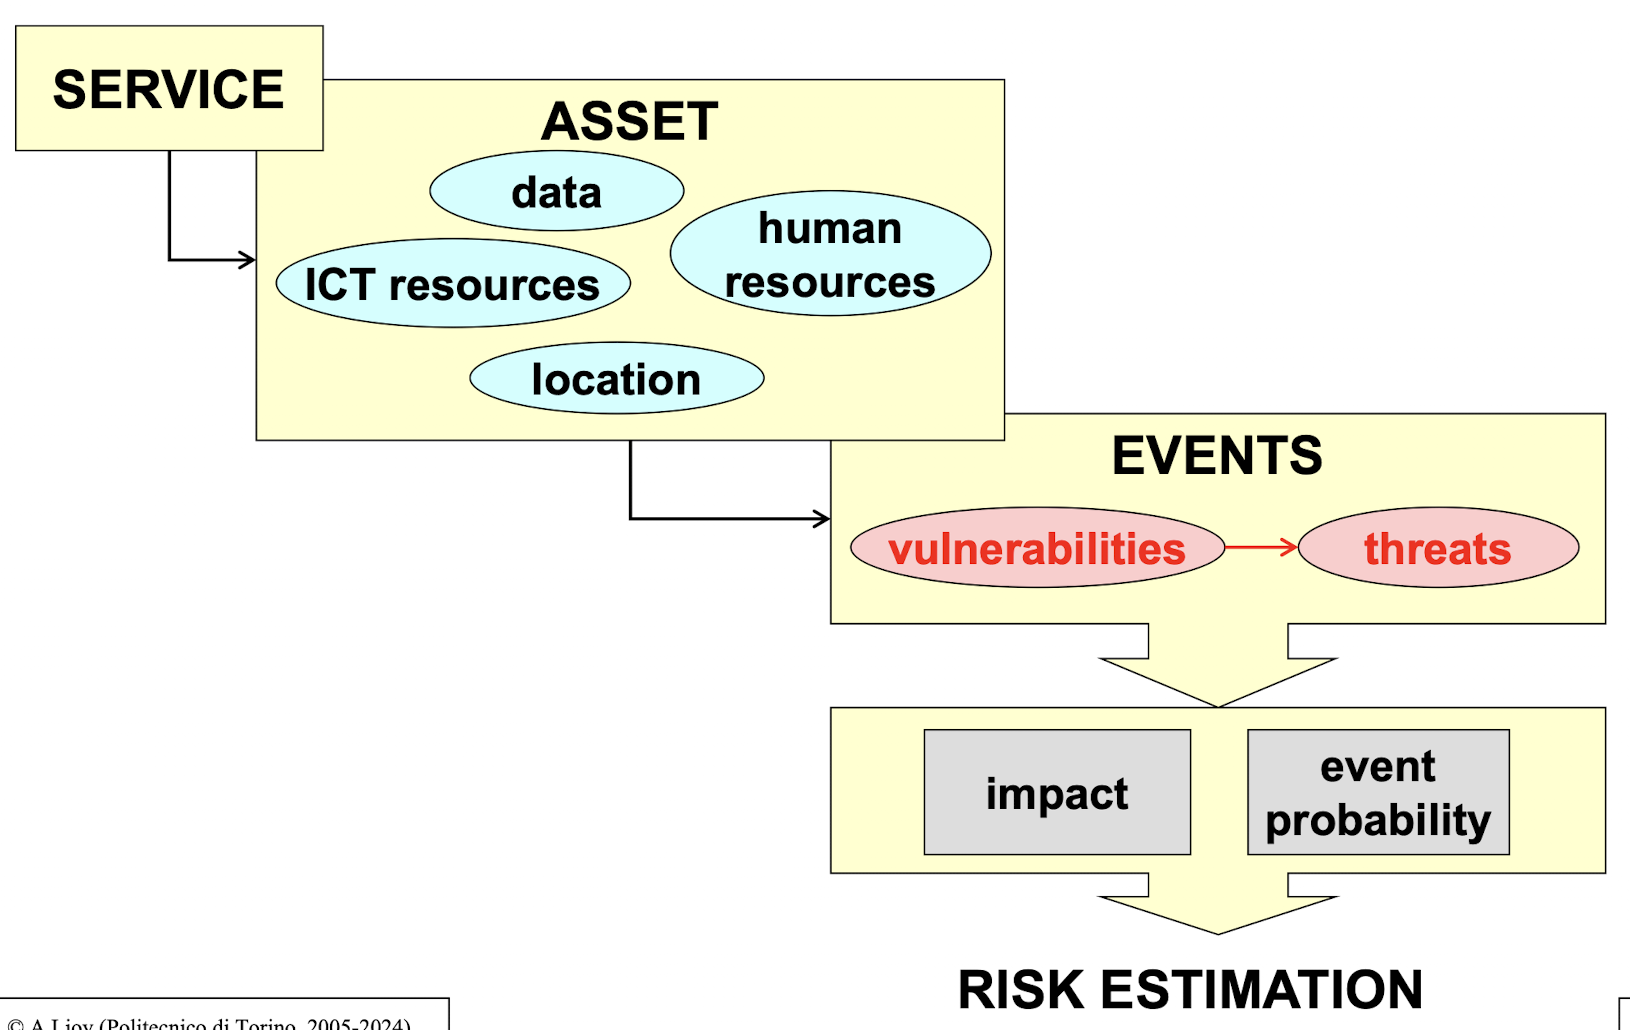
\includegraphics[width=\linewidth]{Images/Introduction/riskEvaluation.png}
        \caption{The risk estimation process}
    \end{figure}
\end{multicols}

Managing threats requires us to \textbf{prioritize risks}, considering not only the impact but also the available \textbf{time and budget}\footnote{A risk assessment matrix (or risk heat map) can be useful in this process}.

\begin{figure}[H]
    \centering
    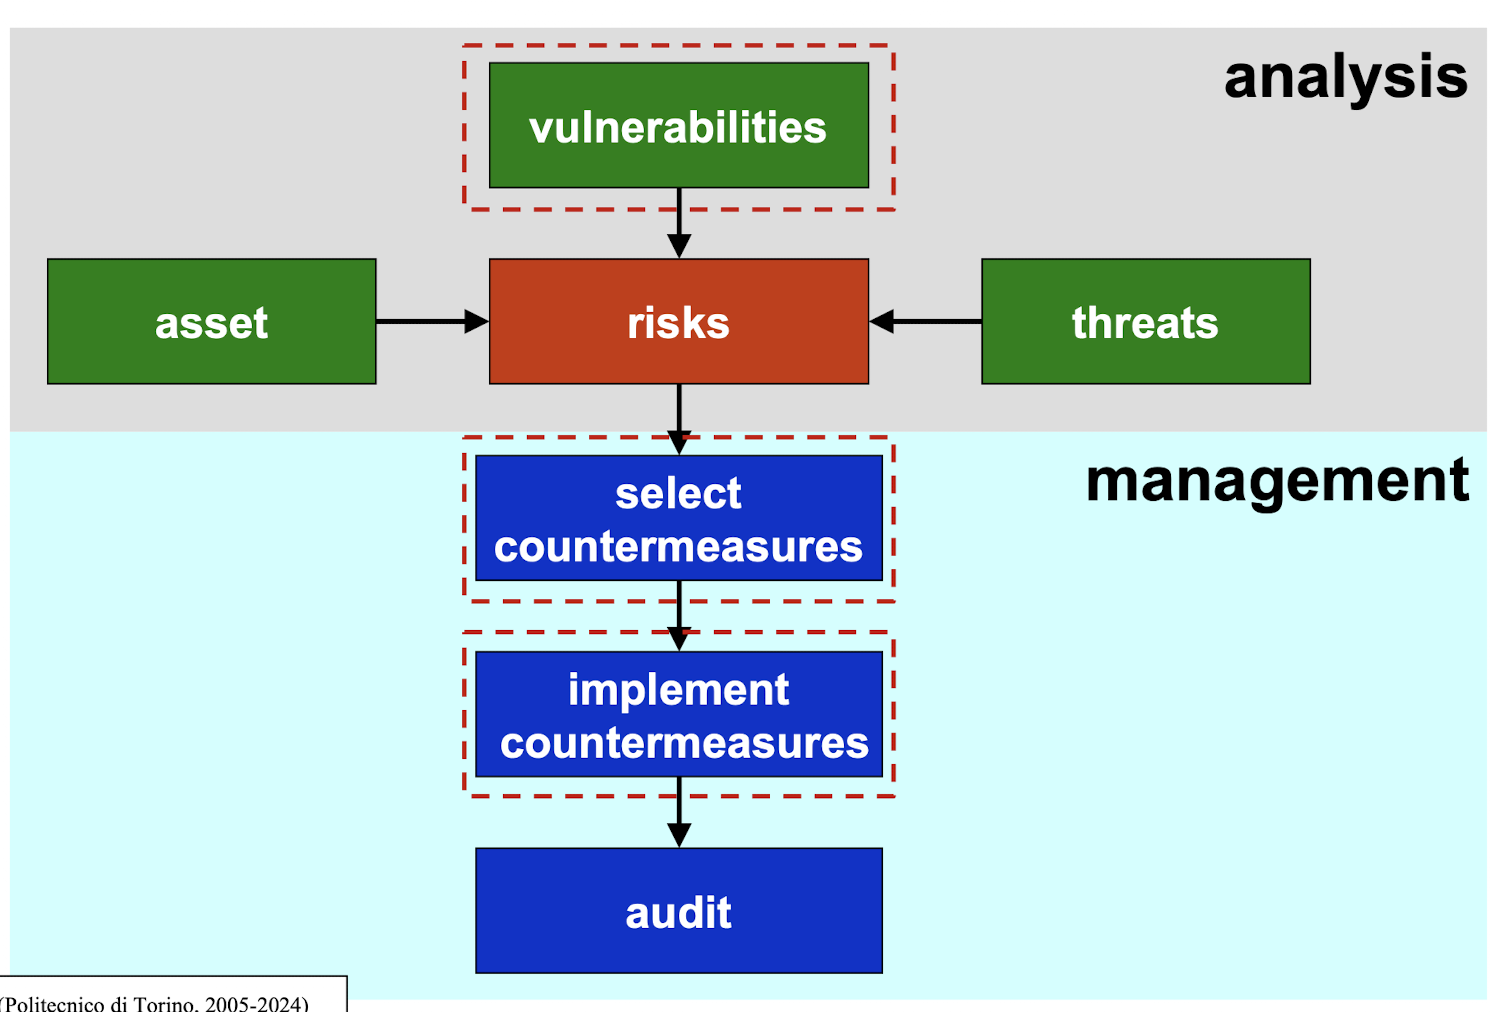
\includegraphics[width=0.5\linewidth]{Images/Introduction/analysisAndManagement.png}
    \caption{Analysis and management of security}
\end{figure}

\subsection{Data Protection}
For each security property always consider the three cases of data protection: data in transit (protected channel), data at rest (protected disk) and data at work (protected memory).

\subsection{Threat Model}
An enemy performs actions based on its position and capabilities. When considering attacks from a positional perspective, we can distinguish between different types of attack vectors: Man In The Middle (MITM), Man At The End (MATE), Man In The Browser (MITB). On the other hand capabilities influence the attack methods and level of sophistication the enemy can employ. For instance, an enemy can act as a passive attacker, merely reading data or traffic without altering it, or as an active attacker, who not only reads but also modifies or injects data into the traffic.

\subsection{Basic Problems}
Modern networks face several technological vulnerabilities that make them susceptible to various security threats. Firstly, network communications are often insecure. Many communications are transmitted in plain text, making them easy to intercept. Additionally, LANs typically operate in broadcast mode, which exposes data to anyone within range, and wireless communications are similarly vulnerable to interception due to the lack of encryption. Geographic connections between locations do not use end-to-end dedicated lines; instead, they rely on shared lines and third-party routers, further compromising security.

Another major issue lies in authentication practices. User authentication mechanisms are generally weak, as they are usually password-based, which is insufficient for robust security. Furthermore, server authentication is often either non-existent or poorly implemented, leaving servers open to unauthorized access.

Lastly, the software running on these networks tends to have numerous bugs. These vulnerabilities can be exploited by attackers, further undermining the security of the system. Addressing these fundamental issues is critical to improving network security and protecting sensitive information.

Non-technological problems in cybersecurity often stem from human factors and system design issues. One major challenge is low problem understanding or awareness; many users are unaware of the risks and threats they face online, which makes them vulnerable to attacks. Additionally, human error plays a significant role, especially when individuals are overloaded, stressed, or distracted, leading to mistakes such as falling for phishing scams or misconfiguring security settings. Another issue is that human beings have a natural tendency to trust systems and people, which cyberattackers can exploit through social engineering tactics like phishing or pretexting. Moreover, complex interfaces and architectures can mislead users, making it harder for them to identify potential security threats or navigate security features correctly. This can result in inadvertent errors, such as incorrect file permissions or failure to apply security patches.

Lastly, performance decreases due to the application of security measures can discourage users from fully implementing necessary protections, as they may prioritize convenience or speed over safety. These non-technological factors are critical in understanding how cybersecurity vulnerabilities can arise and emphasize the need for user education, simplified interfaces, and effective security practices.

\hfill 
\begin{center}
    Refer to Appendices A and B for a clearer understanding of potential attacks and attack vectors.
\end{center}
\hfill

\subsection{NIST Cybersecurity Framework}
The NIST Cybersecurity Framework is a set of guidelines developed by the National Institute of Standards and Technology (NIST) to help organizations manage and mitigate cybersecurity risks. It provides a flexible, risk-based approach to cybersecurity and is widely used across various industries. The framework is structured around five core functions, which are designed to be applied in a continuous cycle:
\begin{itemize}
    \item Identify: Develop an understanding of the organization’s cybersecurity risks by identifying assets, vulnerabilities, threats, and impacts. This includes understanding business objectives, resources, and risk tolerance.
    \item Protect: Implement safeguards to ensure the delivery of critical infrastructure services. This includes access control, data security, awareness programs, and protective technologies to limit cybersecurity risks.
    \item Detect: Implement monitoring systems to identify cybersecurity incidents. This function involves continuous monitoring for anomalies, events, and potential breaches.
    \item Respond: Develop and implement an action plan for responding to detected cybersecurity incidents. This involves planning and coordination for incident management and mitigation strategies.
    \item Recover: Develop and implement strategies to restore capabilities or services that were impacted by a cybersecurity incident. This ensures that recovery processes are in place for business continuity.
\end{itemize}

\begin{figure}[H]
    \centering
    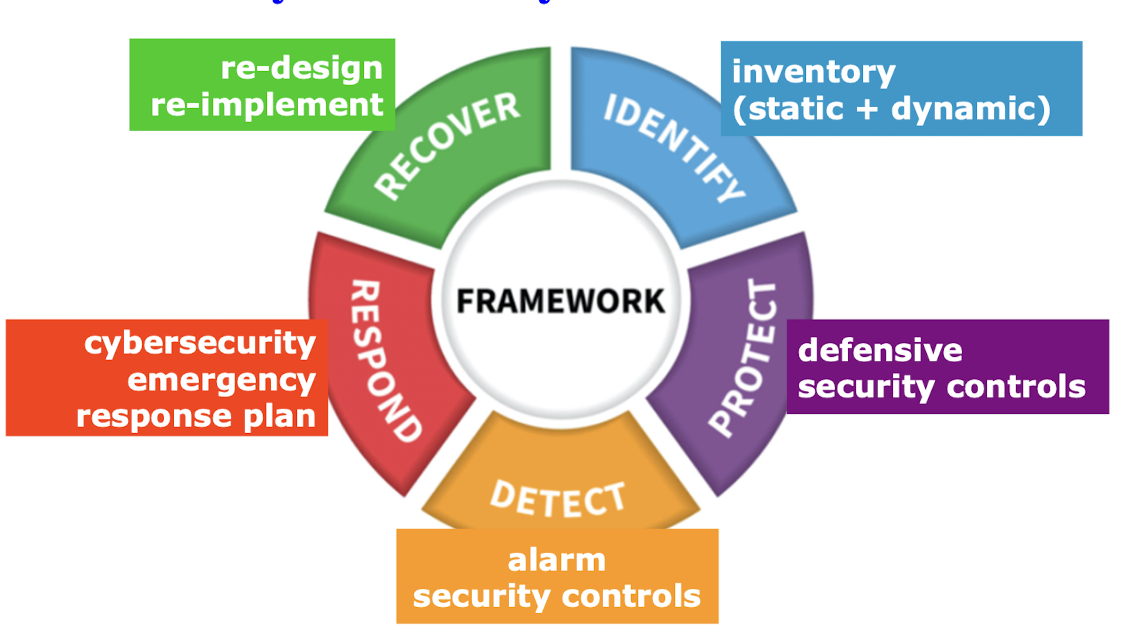
\includegraphics[width=0.5\linewidth]{Images/Introduction/nistFramework.png}
    \caption{NIST cybersecurity framework}
\end{figure}
%\chapter{Cryptographic Techniques}
\cite{02_basic_crypto}.
Cryptography is the practice of securing communication and data by transforming it into a format that is unreadable to unauthorized users. It uses mathematical algorithms to encrypt (scramble) and decrypt (unscramble) information, ensuring confidentiality, integrity, authentication, and non-repudiation in digital communications.

The message in its original, unencrypted form is called plaintext (or cleartext), referred to as P. On the other hand, the message after being encrypted is called ciphertext, referred to as C. 

\section{Symmetric Cryptography}
\begin{center}
    Only one key, shared between the sender and the receiver, is used for both encryption and decryption. 
\end{center}
Pros and cons:
\begin{itemize}
    \item Key distribution problems (lots of keys for a complete pairwise private communication).
    \item Key management problems.
    \item Faster than asymmetric cryptography.
    \item Main utility: data confidentiality.
\end{itemize}



\begin{multicols}{2}

    \textbf{Encrypt Equation}
\begin{equation*}
    \begin{aligned}
        C &= \text{enc}(K, P) \\
          &= \{ P \}_K
    \end{aligned}
\end{equation*}

\hfill

\textbf{Decrypt Equation}
\begin{equation*}
    \begin{aligned}
        P &= \text{dec}(K, C) \\
          &= \text{enc}^{-1}(K, C)
    \end{aligned}
\end{equation*}
    \columnbreak
    
    \begin{figure}[H]
        \centering
        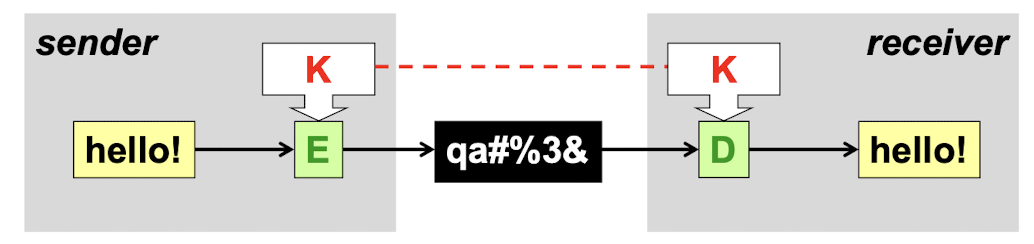
\includegraphics[width=\linewidth]{Images/Cryptography/symmCrypto.png}
        \caption{Example of symmetric encryption}
    \end{figure}
\end{multicols}

\clearpage

\subsection{Symmetric Block Encryption Algorithms}
Block encryption refers to ciphers that process fixed-size blocks of data (e.g., 128 bits for AES) at a time.

\begin{figure}[H]
    \centering
    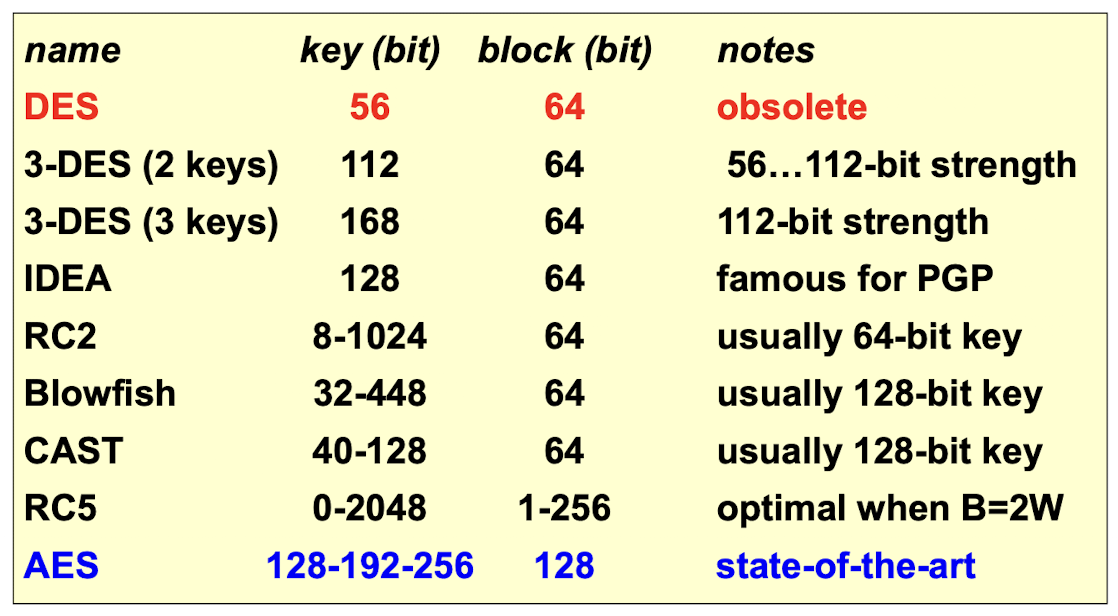
\includegraphics[width=0.5\linewidth]{Images/Cryptography/blockSymm.png}
    \caption{Famous Symmetric Block Encryption Algorithms}
\end{figure}


\subsubsection{Data Encryption Standard}
\begin{center}
    (DES - Obsolete because of short key length)

    56-bit key, 64-bit block.
\end{center}
Is a symmetric-key block cipher that was widely used for data encryption in the past. It was developed in the 1970s by IBM.

The key features are:
\begin{itemize}
    \item Block cipher: DES operates on 64-bit (8 bytes) blocks of data, meaning it encrypts 64 bits of plaintext at a time.
    \item Key length: DES uses a 56-bit (7 bytes) key.
    \item Efficient in hardware: Requires only XOR, shift and permutation.
\end{itemize}

\subsubsection{Triple DES}
\begin{center}
    (3DES or TDES)

    112 or 168-bit key, 64-bit block, EDE mode for backward compatibility.
\end{center}

Is a symmetric-key block cipher that was developed to enhance the security of the original DES.

The key features are:
\begin{itemize}
    \item Block cipher: like DES (8 bytes).
    \item Key Length: 3DES can use either:
    \begin{itemize}
        \item \textbf{Two keys} (2-key 3DES): The first and third keys are the same, resulting in a 112-bit effective key length.
        \item \textbf{Three keys} (3-key 3DES): All three keys are distinct, resulting in a 168-bit effective key length.
    \end{itemize}
    \item Triple encryption: 3DES applies the DES algorithm three times to each data block, using either two (2-key 3DES) or three (3-key 3DES) distinct keys.
    \item Is typically applied in the Encrypt-Decrypt-Encrypt (EDE) mode to achieve compatibility with DES when.
\end{itemize}

\subsubsection*{EDE Mode}
In this mode, the data is first encrypted using the first key, then decrypted using the second key, and finally encrypted again using the third key (if a third key is present). This sequence of operations helps mitigate the vulnerabilities of DES by applying encryption multiple times.

\begin{tcolorbox}[colback=blue!10!white, colframe=blue!50!white, title=Meet-in-the-Middle attack]
    Double application of encryption algorithms is subject to a known plaintext attack named meet-in-the-middle, which allows decrypting data with at most $2^{N+1}$ attempts (the key is N-bit long).
    For more details, refer to Appendix A.
\end{tcolorbox}

\subsubsection{Advanced Encryption Standard}
\begin{center}
    AES.
\end{center}
In order to replace DES.

\begin{itemize}
    \item Symmetric block cipher.
    \item Developed by Joan Daemen and Vincent Rijmen.
    \item Key features:
    \begin{itemize}
        \item Block size: 128 bits.
        \item Key length: 128, 192, or 256 bits.
    \end{itemize}
\end{itemize}

\begin{tcolorbox}[colback=blue!10!white, colframe=blue!50!white]
Ciphers are like wine: the older, the better.
\end{tcolorbox}


\subsection{Application Modes for Block Algorithms}
Block ciphers split the data (plaintext) into fixed-size blocks.

We should answer a question:
\begin{tcolorbox}[colframe=lightblue]
    \begin{center}
        \textit{Is the size of the data to encrypt smaller or larger than \newline the algorithm's block size?}
    \end{center}
\end{tcolorbox}
    

If the answer is:
\begin{itemize}
    \item Size of the data to encrypt > algorithm's block size: Use Electronic Code Book (ECB) or Cipher Block Chaining (CBC).
    \item Otherwise (size of the encrypted data not a multiple of the block size): Padding, Cipher FeedBack (CFB), Output FeedBack (OFB) or Counter Mode (CTR).
\end{itemize}

\subsubsection{Electronic Code Book}
\begin{center}
    (ECB)
\end{center}

Simple mode of operation for block ciphers. In this mode, the plaintext is divided into fixed-size blocks, and each block is encrypted independently using the same key.

\begin{multicols}{2}
    \begin{equation*}
        \boxed{C_i = enc \ (K, P_i)}
    \end{equation*}
    \begin{figure}[H]
        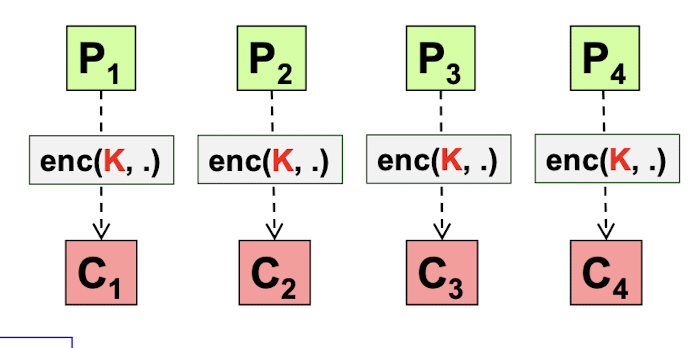
\includegraphics[width=\linewidth]{Images/Cryptography/ECBEncrypt.png}
        \caption{ECB encrypting.}
    \end{figure}
    \columnbreak
    \begin{equation*}
        \boxed{P_j = \text{enc}^{-1}(K, C_j)}
    \end{equation*}
    \begin{figure}[H]
        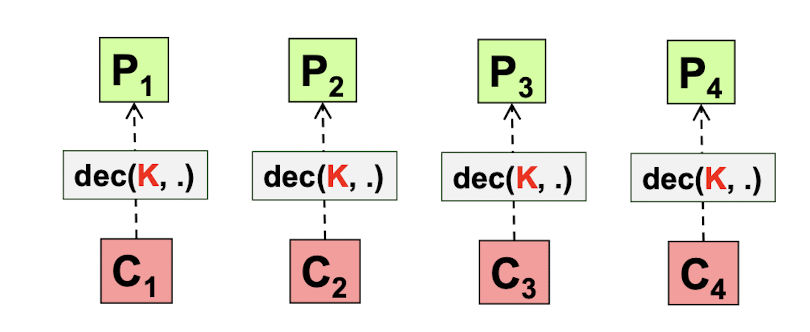
\includegraphics[width=\linewidth]{Images/Cryptography/ECBDecrypt.png}
        \caption{ECB decrypting.}
    \end{figure}
\end{multicols}

Key features:
\begin{itemize}
    \item Should not be used for long messages because swapping two blocks of ciphertext goes undetected.
    \item Each block is encrypted separately with the block cipher using the same key.
    \item The encrypted blocks are concatenated to produce the ciphertext.
    \item Identical plaintext blocks produce identical ciphertext blocks, which can lead to patterns in the ciphertext that may be exploited in cryptanalysis.
    \item If there is an error in one ciphertext block  $C_j$ , only the corresponding plaintext block  $P_j$  will be affected during decryption.
\end{itemize}

\clearpage
\subsubsection{Cipher Block Chaining}

\begin{center}
    (CBC)
\end{center}
Mode of operation for block ciphers that provides better security than Electronic Codebook (ECB). It involves chaining the encryption of each block with the previous block's ciphertext, which helps obscure patterns in the ciphertext.


\begin{multicols}{2}
    \begin{equation*}
        \boxed{C_i = enc \ (K, P_i \oplus C_{i-1})}
    \end{equation*}
    \begin{figure}[H]
        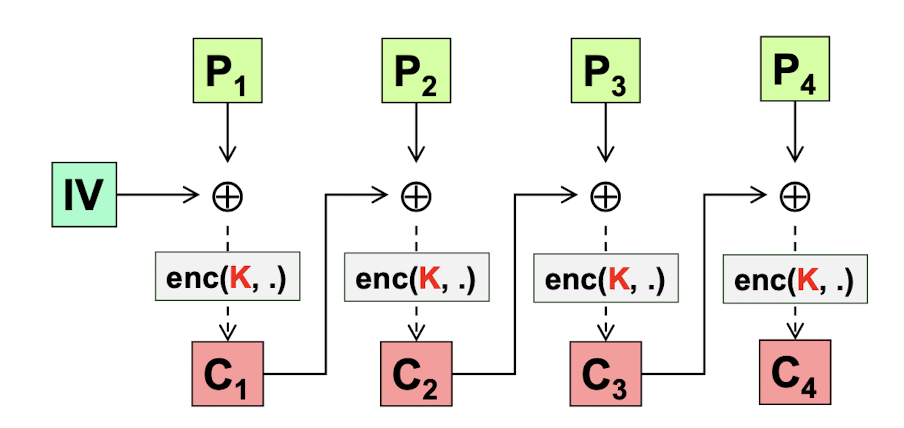
\includegraphics[width=\linewidth]{Images/Cryptography/CBCEncrypt.png}
        \caption{ECB encrypting.}
    \end{figure}
    \columnbreak
    \begin{equation*}
        \boxed{P_j = \text{enc}^{-1}(K, C_j) \oplus C_{j-1}}
    \end{equation*}
    \begin{figure}[H]
        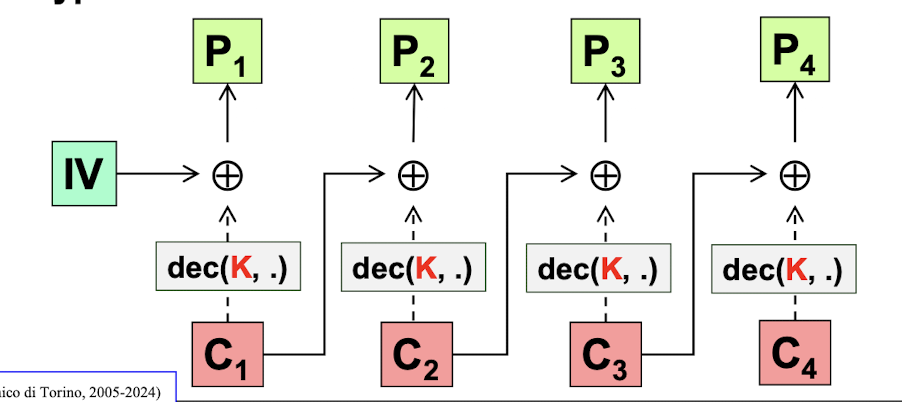
\includegraphics[width=\linewidth]{Images/Cryptography/CBCDecrypt.png}
        \caption{ECB decrypting.}
    \end{figure}
\end{multicols}

Key features:
\begin{itemize}
    \item Requires an Initialization Vector (IV=$C_0$).
    \item XOR between ciphertexts and plaintexts.
    \item If there is an error in a ciphertext block $C_j$ it will affect the decryption of two blocks of plaintext:
    \begin{itemize}
        \item The current block $P_j$ will be corrupted because the error will be decrypted into some incorrect plaintext. 
        \item The next block  $P_{j+1}$  will also be corrupted because the error will propagate into the XOR operation with the next ciphertext block  $C_{j+1}$.
    \end{itemize} 
\end{itemize}

\clearpage

\subsubsection{Padding}
\begin{center}
    Scopes: aligning, filling. Always add data to a block.
\end{center}

Padding is used in block cipher encryption schemes to handle plaintext that is not an exact multiple of the block size. Since block ciphers operate on fixed-size blocks, any plaintext that does not fit into the required block size needs to be padded.
\begin{figure}[H]
    \centering
    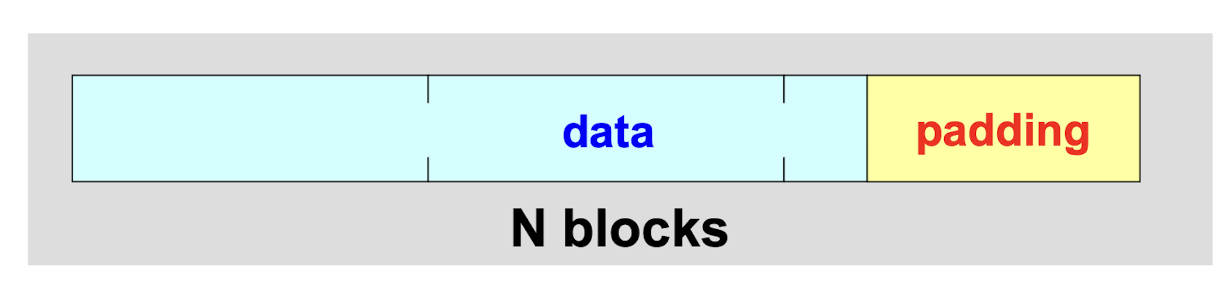
\includegraphics[width=0.5\linewidth]{Images/Cryptography/padding.png}
    \caption{Padding Mode}
    
\end{figure}

\subsubsection*{Padding Techniques}
\begin{itemize}
    \item Original DES Padding: bit pattern that started with a 1 bit, followed by many 0 bits.
    \item One byte with value 128 (0x80) followed by null bytes.
    \item Last byte indicates padding length.
    \item Padding with explicit length:
    \begin{itemize}
        \item Null bytes, with the last byte indicating the padding length.
        \item Only null bytes. \textcolor{Blue}{Schneier}
        \item Bytes with value equal to Length. \textcolor{Blue}{SSL/TLS}
        \item Random bytes. \textcolor{Blue}{SSH2}
        \item Sequential numbers starting from 0x01. \textcolor{Blue}{IPSec/ESP}
        \item Each byte is the $Length-1$.
    \end{itemize}
\end{itemize}

\subsubsection*{Some Keynotes}
\begin{itemize}
    \item Minimal integrity control: If the key is incorrect or data were manipulated, the padding bytes will become incoherent.
    \item Typically applied to large data, on the last fragment.
    \item If the data length D is less than the block size B, ad-hoc techniques like CFB, OFB, or CTR are preferred instead of padding.
    \item \textbf{Even if the plaintext is an exact multiple of the block size, padding is still required to avoid errors in the interpretation of the last block.}
\end{itemize}

\subsubsection{Cipher Text Stealing}
\begin{center}
    (CTS)
\end{center}
Allows the use of block algorithms without adding new data to a block (e.g. padding).

Process (using CTS-ECB):
\begin{itemize}
    \item Uses CBC until the last block of the plaintext.
    \item The second-to-last block is encrypted and divided into two parts (head + tail, the tail is the same size as the gap of the plaintext $n$).
    \item The last (partial) block is filled with the tail from the second-to-last block.
    \item The "new" last block (old last block + tail, now "full") is encrypted.
    \item After encryption, the positions of the last and second-to-last block (only the "head") are swapped.
\end{itemize}
This method is particularly useful when the size of the data cannot be increased after encryption, such as in storage encryption.

\textbf{However, the computation time increases slightly}.

\begin{multicols}{2}

    \begin{figure}[H]
        \centering
        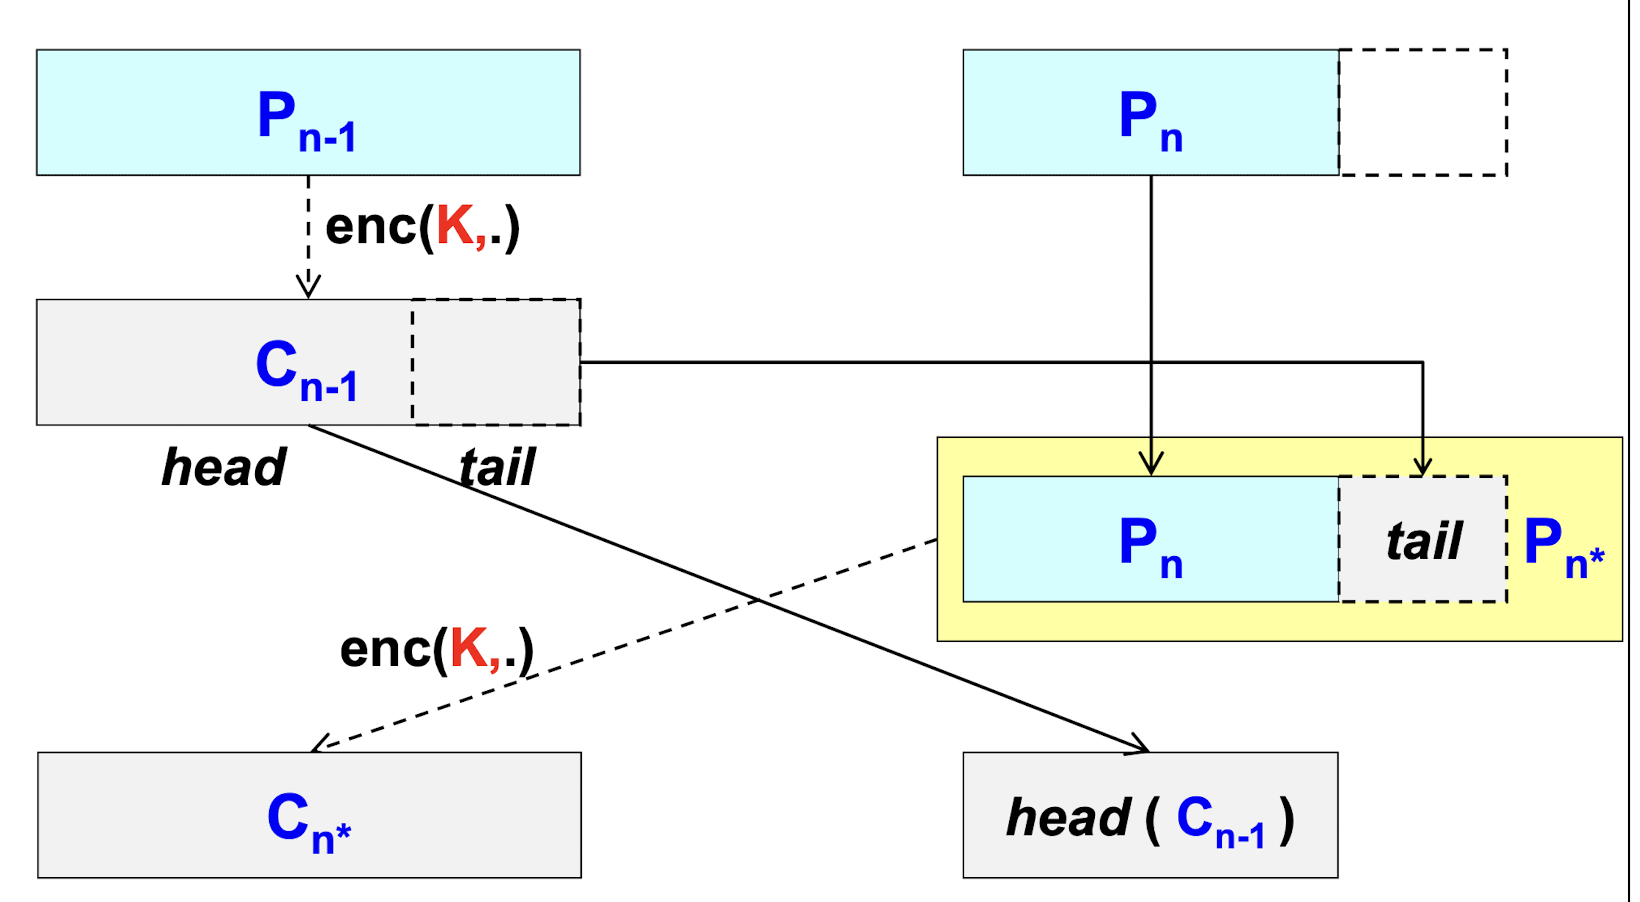
\includegraphics[width=\linewidth]{Images/Cryptography/CTS_ECB.png}
        \caption{CTS with ECB}
    \end{figure}

    \columnbreak

    \begin{figure}[H]
        \centering
        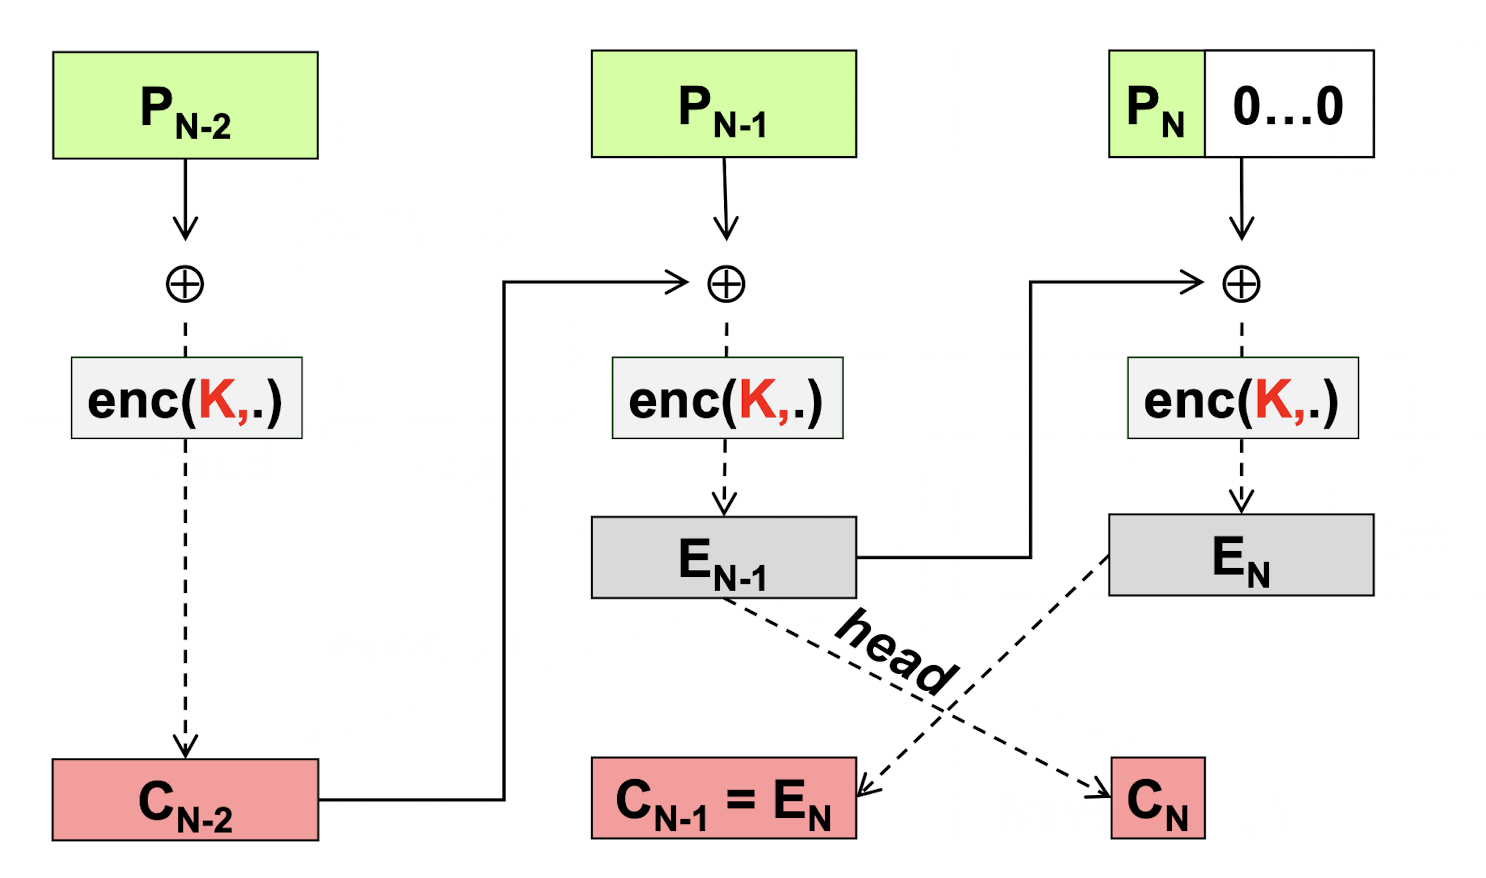
\includegraphics[width=\linewidth]{Images/Cryptography/CTS_CBC.png}
        \caption{CTS with CBC}
    \end{figure}
    
\end{multicols}

\clearpage 
\subsubsection{Counter Mode}
\begin{center}
    (CTR)
\end{center}
Requires a \textbf{nonce} and a \textbf{counter}, combined to generate the input block.

Key features:
\begin{itemize}
    \item The nonce is a random number that should never be reused with the same data.
    \item The counter is a value that is incremented for each block.
    \item The input block is encrypted using the block cipher, generating a fixed-size encrypted "unique" block.
    \item The leftmost group\footnote{Meaning the first N bits, based on the required $plaintext\_size$.} is extrapolated from the block and are XORed with the corresponding $P_i$ group, which in turn generates the corresponding $C_i$ group.
    \item The same process is repeated for each successive plaintext group, with the counter incremented each time.
\end{itemize}

\begin{figure}[H]
    \centering
    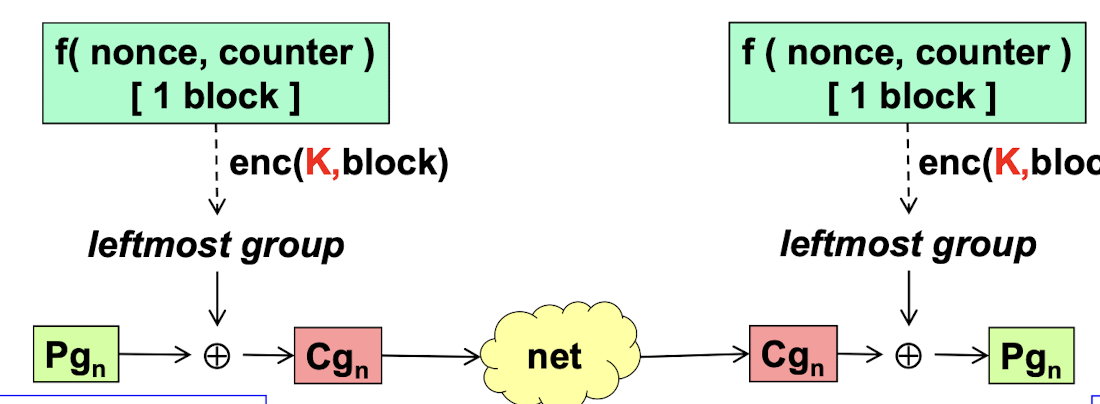
\includegraphics[width=0.6\linewidth]{Images/Cryptography/CTR_ENC.png}
    \caption{CTR Mode}
\end{figure}


\subsection{Symmetric Stream Encryption Algorithms}
\begin{center}
    Byte-by-byte(or bit-by-bit) encryption.

    No fixed-size block boundaries.
\end{center}
Stream encryption refers to ciphers that process data one bit or byte at a time.





\begin{multicols}{2}


    Main features:
    \begin{itemize}
        \item Ideal algorithm: One-Time Pad (OTP), requires a key as long as the plaintext to protect.
        \item Real algorithms: Use pseudo-random number generators (PRNGs) to generate a key stream, \textbf{synchronized} between sender and receiver.
        \item Modern: Salsa20, ChaCha20.
    \end{itemize}
\columnbreak

\begin{figure}[H]
    \centering
    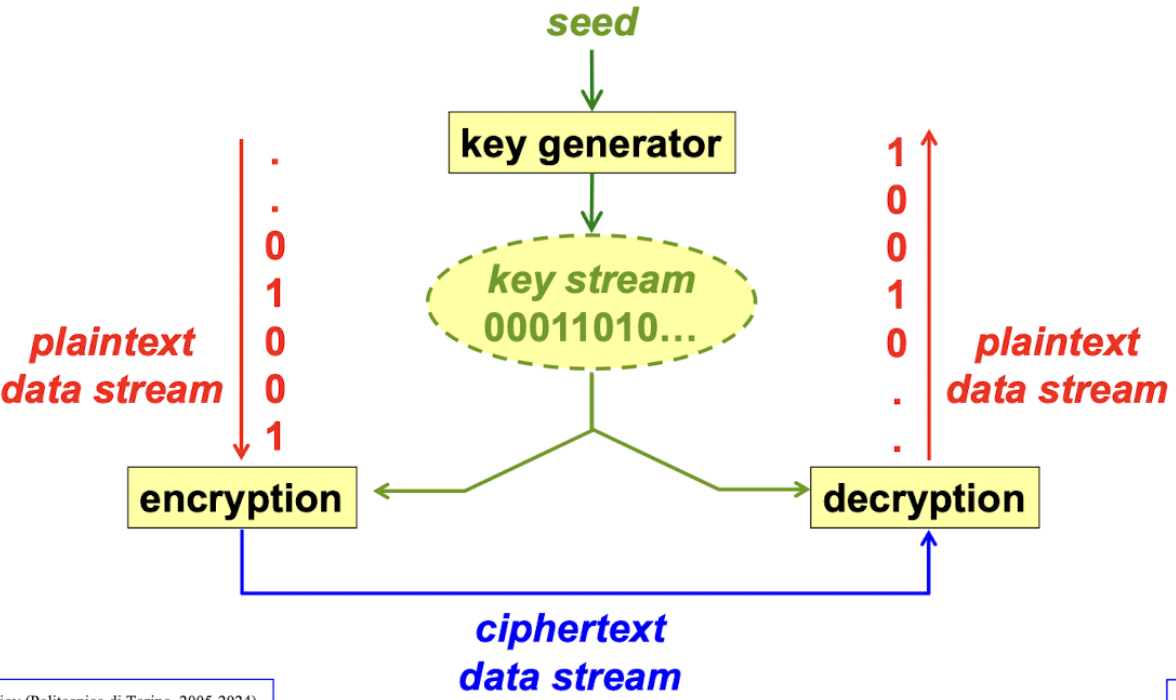
\includegraphics[width=\linewidth]{Images/Cryptography/Stream_Cipher.png}
    \caption{Stream (real) algorithm process.}
\end{figure}
\end{multicols}

\subsubsection{Salsa20}
\begin{center}
    128 or 256-bit Key.
\end{center}

Key features:
\begin{itemize}
    \item 128 or 256-bit Key.
    \item Base operation: 32-bit ARX (Addition, Rotation, XOR).
    \item Base function: f(Key \textcolor{Blue}{(256 bits)}, Nonce \textcolor{Blue}{ 64}, Counter \textcolor{Blue}{ 64}) = 512-bit keystream block.
    \item Can process 64-byte blocks of data.
    \item Allows random access decryption: Since each block is encrypted independently, it is possible to decrypt any block at random without needing to decrypt the preceding blocks.
    \item Can securely encrypt $64B \cdot 2^{64}$ blocks of data with a single key and nonce pair.
\end{itemize}
\subsubsection{ChaCha20}
An improved version of Salsa20, designed to provide better security and performance. So inherit the same features as Salsa20.
\begin{center}
    ChaCha20 and Poly1305 for IETF protocols.
\end{center}
Slightly modifications to the original specification:
\begin{itemize}
    \item 96 bit nonce (from 64).
    \item 32 bit lock counter (from 64).
    \item Hence, a limit of $2^{32} \cdot \ 64$ byte blocks. That corresponds to 256 GB of data (amount of data that can be encrypted with a single key and nonce pair) with a 64-byte block size.
\end{itemize}

\section{Comparison of Symmetric Ciphers}



\begin{multicols}{2}

    Stream algorithms:
    \begin{itemize}
        \item Works on variable length data stream (faster computation).
        \item Need a synchronized key stream (synch problems between the parties).
        \item Reliable pseudo random number generator (PRNG).
    \end{itemize} 
\columnbreak

Block algorithms:
\begin{itemize}
    \item Split data into fixed-size blocks (slower computation).
    \item Attacks based on the mode of operation (e.g. ECB).
    \item May be used padding, so additional data to the message.
\end{itemize}
\end{multicols}

\section{Kerchoffs' Principle}
\begin{quotation}
    If the keys are kept secret, managed securely (well-designed algorithm and executed by a trusted party), and are long enough, the system remains secure even if the encryption and decryption algorithms are publicly known. 
\end{quotation}
    This is because, without access to the keys, an attacker cannot decrypt the data. In fact, making the algorithms public allows the cryptographic community to rigorously test and analyze them for potential weaknesses, improving the overall security of the system.


\subsection*{Attempts to Perform an Exhaustive Search}
Assuming that Kerchoffs' Principle is respected. Considering a key of length N bits.

\dots The only possible attack is the brute force (exhaustive search) attack, which requires $2^N$ attempts.

\[
    \boxed{T \propto 2^N}
\]

\subsection{Key Distribution for Symmetric Cryptography}
\raggedcolumns
\begin{multicols}{2}

\noindent For a complete pairwise private communication between N parties, we need:
\begin{center}
    $\boxed{\displaystyle\frac{N \cdot (N-1)}{2}}$ keys.
\end{center}

\columnbreak

    \begin{figure}[H]
        \centering
        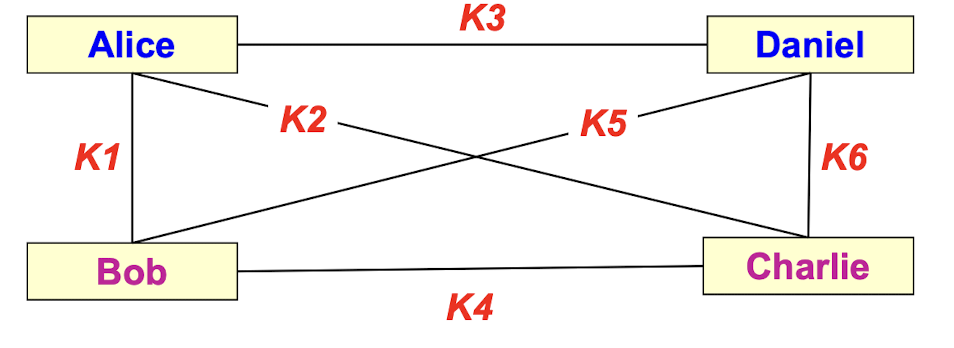
\includegraphics[width=\linewidth]{Images/Cryptography/key_dist_symm.png}
        \caption{Key Distribution}
    \end{figure}
\end{multicols}


Distribution Methods:
\begin{itemize}
    \item Out-Of-Band (OOB): Keys are exchanged using a separate, secure communication channel (e.g., in person or using a different secure network).
    \item Key exchange algorithms.
\end{itemize}


\section{Minimum Acceptable Key Length (2025)}
\begin{itemize}
    \item 128 bits for symmetric algorithms.
    \item 2048 bits for asymmetric algorithms.
    \item 256 bits for cryptographic hash functions.
\end{itemize}
\begin{figure}[H]
    \centering
    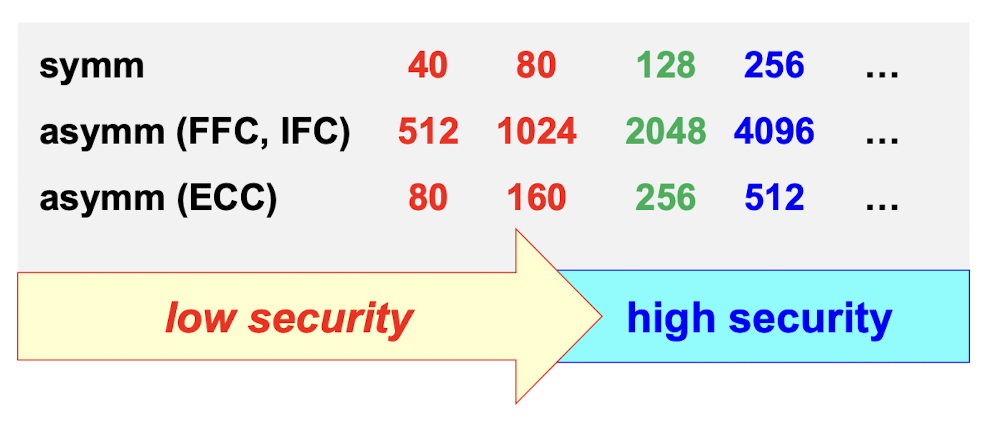
\includegraphics[width=0.5\linewidth]{Images/Cryptography/crypto_key_lens.png}
    \caption{Key length of cryptographic algorithms}
\end{figure}

\section{Asymmetric Cryptography}
\begin{center}
    Used for confidentiality without shared secrets or digital signatures.
\end{center}
AKA public-key cryptography.
Each person has a different key pair (PK, SK). Keys in the pair have inverse functionality: what one key encrypts, the other key decrypts. Private key must be kept secret. Public key should be shared as widely as possible.

\noindent Main features:
\begin{itemize}
    \item Asymmetric encryption is slower than symmetric encryption.
    \item Problems with PK-certificate distribution (validity-check, slow process of certification).
    \item Main algorithms: RSA, DSA.
\end{itemize}


\subsection*{Example of Asymmetric Encryption}
Consider a scenario where Alice wants to send a confidential message to Bob using asymmetric encryption. The steps are as follows:

\begin{enumerate}
    \item Bob generates a key pair: a public key (PK\textsubscript{Bob}) and a private key (SK\textsubscript{Bob}).
    \item Bob shares his public key (PK\textsubscript{Bob}) with Alice.
    \item Alice encrypts her message (M) using Bob's public key (PK\textsubscript{Bob}):
    \begin{verbatim}
        Alice > Bob: C = enc(PKBob, Message)
    \end{verbatim}
    \item Alice sends the ciphertext (C) to Bob.
    \item Bob decrypts the ciphertext (C) using his private key (SK\textsubscript{Bob}):
    \begin{verbatim}
        Bob > Alice: dec(SKBob, C) = Message
    \end{verbatim}
\end{enumerate}

This ensures that only Bob can decrypt the message, as only he has the corresponding private key.

\begin{figure}[H]
    \centering
    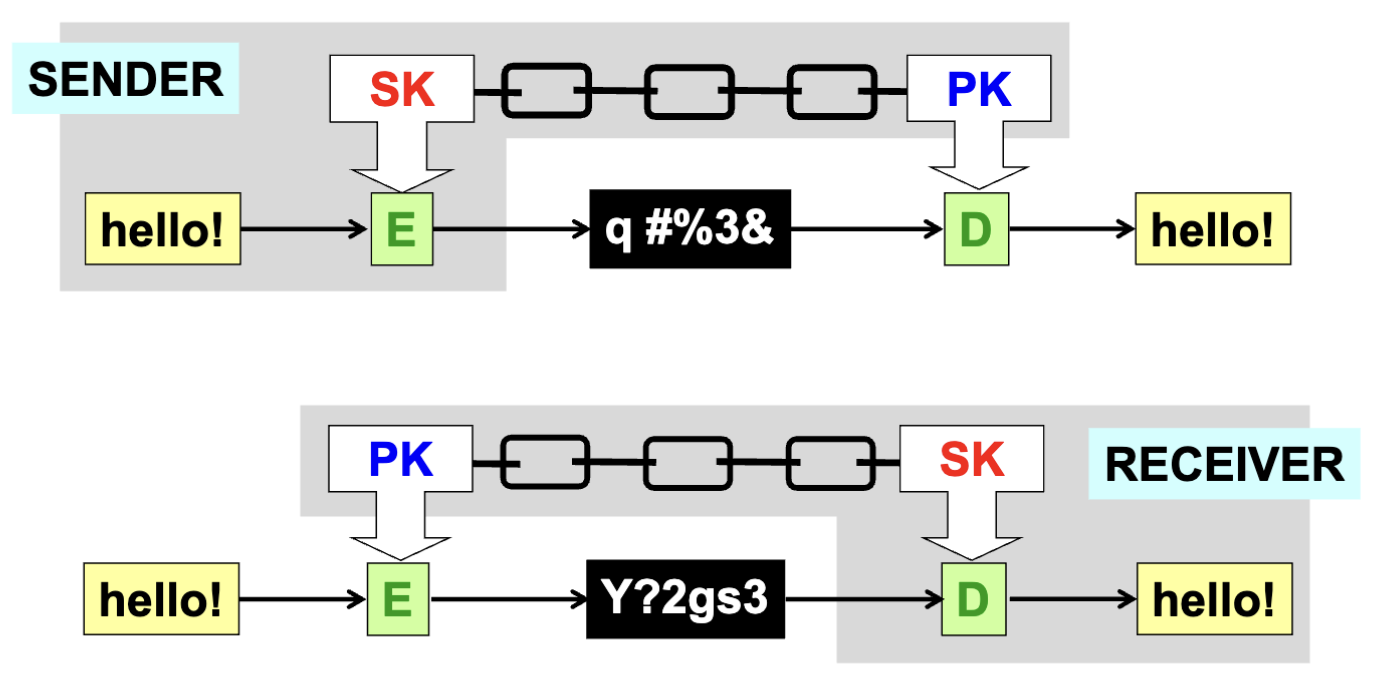
\includegraphics[width=0.5\linewidth]{Images/Cryptography/asymmCrypto.png}
    \caption{Example of asymmetric encryption}
\end{figure}


\subsection{Digital Signature - The Idea}
\begin{center}
    Authentication (but still no integrity and no repudiation).
\end{center}
\begin{tcolorbox}[colback=red!10!white, colframe=red!70!black, coltitle=white, title=Beware]
The idea has no concreteness (and actual dsig is more complex), at the exam you will explain the REAL implementation.
\end{tcolorbox}
\begin{center}
Asymmetric encryption of data made with the private key of the sender. \\ 
Look at the "Authentication by Digest and Asymmetric Encryption" section for further explanation.
\end{center}

Key features:
\begin{itemize}
    \item The idea provides data authentication.
    \item The actual digital signature offers also integrity and non-repudiation.
\end{itemize}


\begin{figure}[H]
    \centering
    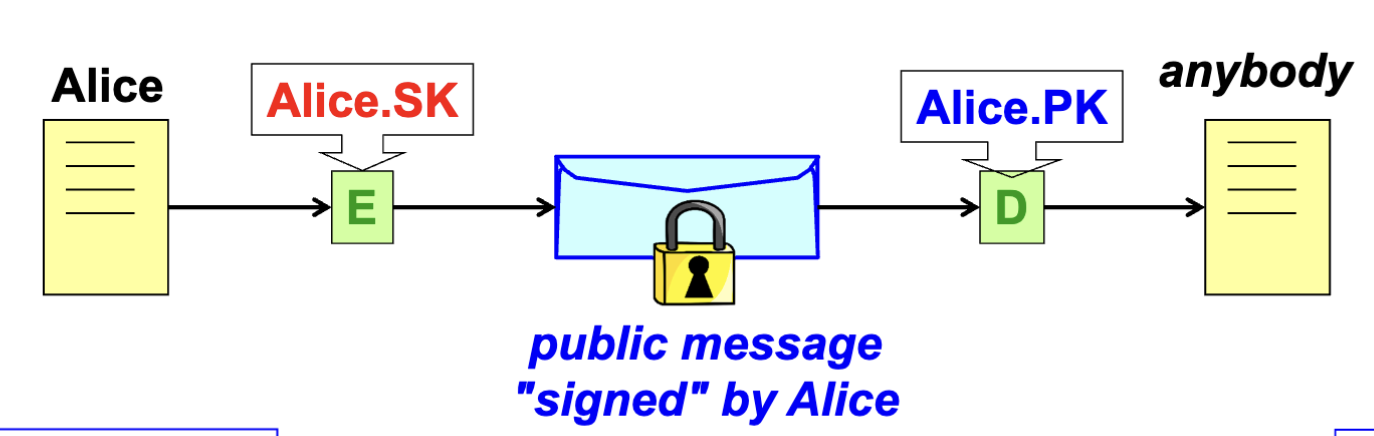
\includegraphics[width=0.5\linewidth]{Images/Cryptography/basic_digital_signature.png}
    \caption{Basic idea of digital Signature}
\end{figure}


\subsection{Asymmetric Cryptography Algorithms}
Minimum acceptable key length: 2048 bits.

\subsubsection{Rivest-Shamir-Adleman}
\begin{center}
    (RSA)
\end{center}

Its security relies on the difficulty of factoring large composite numbers.\footnote{Reference appendix A, Factorization Attack.}

\begin{center}
    \textbf{The Algorithm}
\end{center}

Main features:
\begin{itemize}
    \item Public module $N = P \cdot Q$, known to anybody.
    \begin{itemize}
        \item $P, Q$ are prime numbers, large and secret (deleted/discarded after their usage, dangerous if someone can find them!).
    \end{itemize} 
    \item Exponents:
    \begin{itemize}
        \item Public exponent: $E$. Arbitrarily chosen, $1 < E < \phi(N)$ (Euler's totient function).
        \[
            \phi(N) = (P-1) \cdot (Q-1)
        \]
        \item Private exponent: $D$. Calculated as $D = E^{-1}\cdot \mod \phi(N)$\footnote{Modulus as the remainder of the integer division.}.
    \end{itemize}
    \item Keys:
    \begin{itemize}
        \item Public key: $(N, E)$.
        \item Private key: $(N, D)$.
        \item Key length: size of the public module.
    \end{itemize}
\end{itemize}

\noindent\textcolor{Red}{Be aware:} RSA may cipher/decipher only data whose value is less than the value of the module N (it's a sort of block algorithm, with block size equal to the key size).

\noindent Main aspects:
\begin{itemize}
    \item Plaintext\_size: P < N.
    \item Encryption: $C = P^E \mod N$.
    \item Decryption: $P = C^D \mod N$.
    \item The roles of $E$ and $D$ are interchangeable.
    \[
        (C)^D \mod N = (P^D)^E \mod N = P
    \]
\end{itemize}

\begin{center}
    \textbf{Computational Optimization}
\end{center}

Usually, all public keys have E=3, 17 or 65537. Because the power operation is very easy on numbers with two bits set to one.
\begin{itemize}
    \item High speed of the encryption operation and in signature verification.
\end{itemize}
Operations involving the private key (signing and decrypting) are slow. So, the CRT (\textbf{Chinese Remainder Theorem}) is used to speed up 4x the decryption operation.
Thanks to the equivalence: 
\[
    f(x) \mod N = (f(x) \mod P)\ \&\ (f(x) \mod Q)
\]


\subsubsection{Digital Signature Algorithm}
\begin{center}
    (DSA)
\end{center}
Used for digital signature (Authentication) only: Because it uses a one-way lossy compression function, so original plaintext cannot be recovered.

Main features:
\begin{itemize}
    \item Modular exponentiation.
    \item For encryption, use the El-Gamal algorithm.
\end{itemize}

\begin{tcolorbox}[colback=red!10!white, colframe=red!70!black, coltitle=white, title=Beware]
    Algorithm based on discrete logarithms. It is mainly vulnerable due to mathematical weaknesses or implementation flaws.\footnote{Reference appendix A, Logarithmic Attacks.}
\end{tcolorbox}

\clearpage

\section{Keys Distribution}

\noindent How to share the public key:
\begin{enumerate}
    \item Exchange OOB (Out-of-bound, e.g. manually).
    \item Public-key certificate (aka digital certificate).
\end{enumerate}

In order to exchange a shared secret (symmetric key) we can use:
\begin{enumerate}
    \item Exchange OOB.
    \item Asymmetric cryptography.
    \item Diffie-Hellman (DH) key exchange.
    \item Elliptic Curve Cryptography (ECC).
\end{enumerate}

\subsection{Shared Secret Key Exchange by Asymmetric Algorithms}
Confidentiality without shared secrets is often used to send the secret key for symmetric encryption. In the top branch of the figure, X sends the encrypted message to Y using the shared key (symmetric encryption). In the bottom branch, X sends the secret key to Y using Y's public key (asymmetric encryption).

\begin{figure}[H]
    \centering
    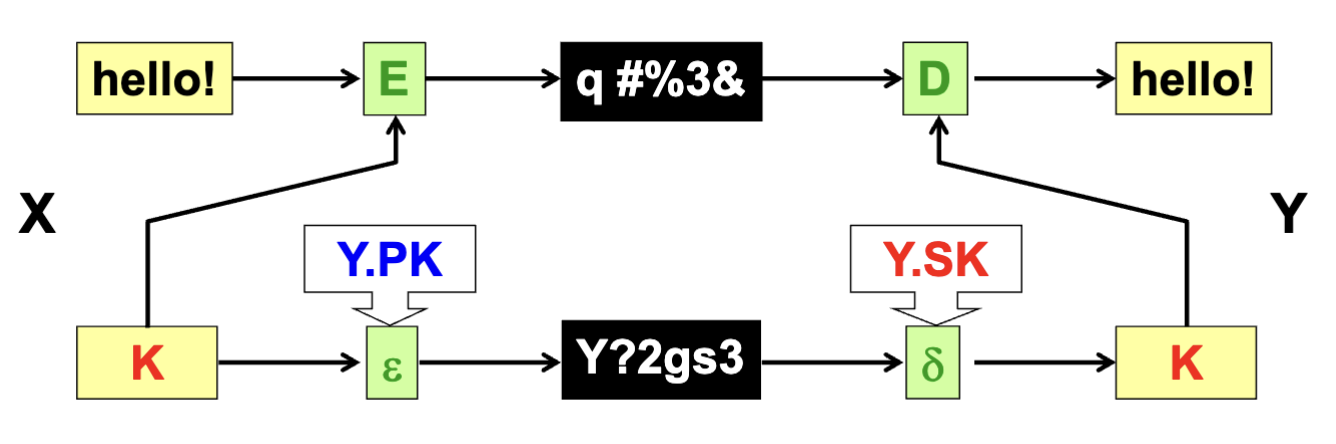
\includegraphics[width=0.7\linewidth]{Images/Cryptography/pk_exchange.png}
    \caption{Secret key exchange by asymmetric algorithms}
\end{figure}

\clearpage

\subsection{Diffie-Hellman Key Exchange}
\begin{center}
    (DH) - Modular Arithmetic.
\end{center}
Main features:
\begin{itemize}
    \item Frequently used to agree on a secret key (key agreement protocol).
    \item Resistant to sniffing attacks.
    \item If the attacker can manipulate the data then it is possible to make a man-in-the-middle attack.\footnote{Reference appendix A}
    \begin{itemize}
        \item To avoid this, the Diffie-Hellman key exchange is often combined with a digital signature algorithm (authentication).
        \item We need certificates for DH keys.
        \item Authenticated DH is MQV (Menezes-Qu-Vanstone).
    \end{itemize}
\end{itemize}

\begin{center}
    \textbf{The Algorithm}
\end{center}
\begin{multicols}{2}
    \begin{center}
        \boxed{\textbf{A}}
        \vspace{0.2cm}
        \hrule
    \end{center}

\columnbreak
\columnseprule=1pt

    \begin{center}
        \boxed{\textbf{B}}
        \vspace{0.2cm}
        \hrule
    \end{center}
    
\end{multicols}

\begin{center}
    A and B agree on two numbers: a large prime number P and a base G (typically 2,3 or 5). Such that:
    \[
        1 < G < P
    \]
    \textcolor{Blue}{(The number of bits of P is the key length)}
\end{center}

\begin{multicols}{2}
    \centering
    Arbitrarily chooses a secret number (integer) x > 0.
    \[
        X= G^x \mod P
    \]
    \columnseprule=1pt
    \columnbreak
    
    Arbitrarily chooses a secret number (integer) y > 0.
    \[
        Y= G^y \mod P
    \]
\end{multicols}

\begin{center}
    A and B exchange (publish) X and Y.
\end{center}

\begin{multicols}{2}
    \centering
    Calculates the shared secret key: \\ $K_A = Y^x \mod P$.
    
    \columnseprule=1pt
    \columnbreak

    Calculates the shared secret key: \\ $K_B = X^y \mod P$.
\end{multicols}

\vspace{1 cm}

So the shared key derived by two parties is: $K_A = K_B=G^{x\cdot y}\mod P$.

\subsection{Elliptic Curve Cryptography}
\begin{center}
    (ECC)
\end{center}
Main features:
\begin{itemize}
    \item Instead of using modular arithmetic, the operations are executed on the surface of a 2D (elliptic) curve. So, the pair of numbers is generated by the curve's equation. 
    \item Only the curve's equation is public.
    \item Digital signature: ECDSA.
    \item Key exchange: ECDH.
    \item Authenticated key agreement: ECMQV (currently patented).
    \item Key distribution: EC Integrated Encryption Scheme (ECIES).
\end{itemize}

\begin{center}
    \textbf{Arithmetics on Elliptic Curves}
\end{center}

Considering a curve: $y^2 = x^3 + ax + b \pmod{p}$ over a finite field\footnote{The arithmetic is performed over a finite field modulo a prime number  p .} $\mathbb{F}_p$.\\
With the condition\footnote{The condition ensures the curve is non-singular, meaning it does not have any cusps or self-intersections.}: $4a^3 + 27b^2 \neq 0$.\\
Compute $R=(x,y)=P+Q$ given:
\begin{itemize}
    \item $P=(x_P,y_P)$.
    \item $Q=(x_Q,y_Q)$.
\end{itemize}
$x= \lambda^2 - x_P - x_Q$ and $y= \lambda(x_P - x) - y_P$ such that the slope $\lambda$ is:
\begin{itemize}
    \item $\lambda = \frac{y_P - y_Q}{x_P - x_Q}$ if $P \neq Q$.
    \item $\lambda = \frac{3x_P + a}{2y_P}$ if $P = Q$.
\end{itemize}

\vspace{1cm}

So we can compute: Addition of two points and Multiplication of a point by a scalar.
\begin{figure}[H]
    \centering
    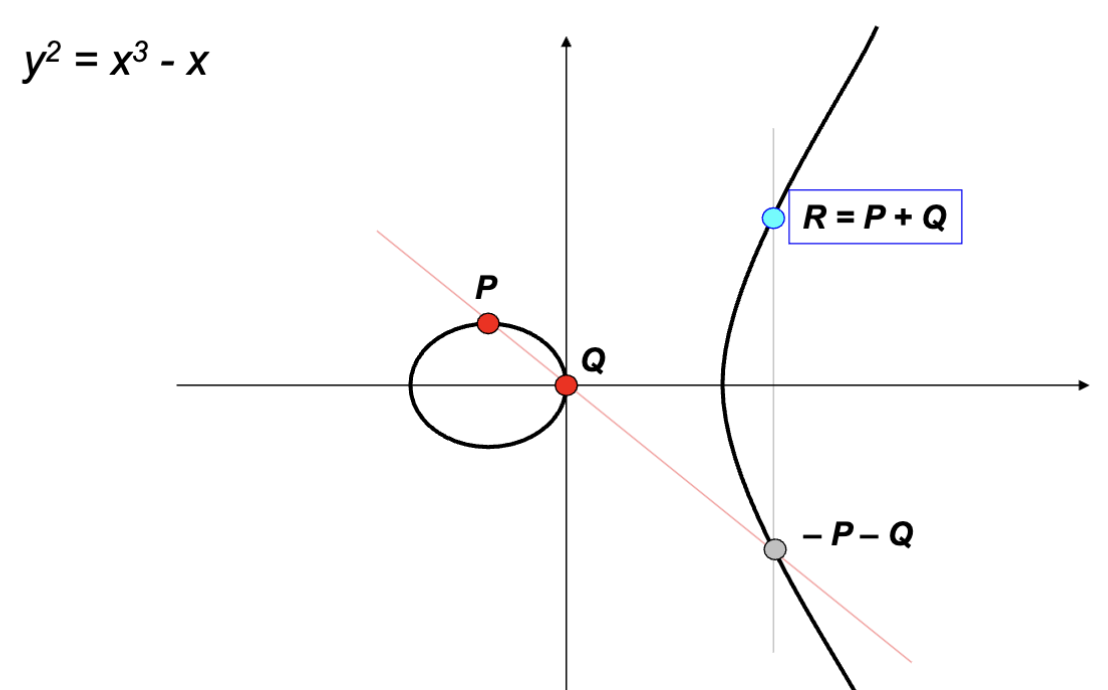
\includegraphics[width=0.5\linewidth]{Images/Cryptography/ec_arith.png}
    \caption{Elliptic Curve arithmetics}
\end{figure}

\begin{tcolorbox}[colback=blue!10!white, colframe=blue!50!white]
    Increased computational complexity can allow for shorter key lengths while maintaining the same level of security.
\end{tcolorbox}

\subsubsection{Elliptic Curve Diffie-Hellman}
\begin{center}
    (ECDH)
\end{center}

\begin{multicols}{2}
    \begin{center}
        \boxed{\textbf{A}}
        \vspace{0.2cm}
        \hrule
    \end{center}

\columnbreak
\columnseprule=1pt

    \begin{center}
        \boxed{\textbf{B}}
        \vspace{0.2cm}
        \hrule
    \end{center}
    
\end{multicols}

\begin{center}
    A and B select the same elliptic curve and a point G of its. Such that:
    \[
         G \in curve
    \]
\end{center}

\begin{multicols}{2}
    \centering
    Arbitrarily chooses a secret number x.
    \[
        X= G \cdot x
    \]
    \columnseprule=1pt
    \columnbreak
    
    Arbitrarily chooses a secret number y.
    \[
        Y= G \cdot y
    \]
\end{multicols}

\begin{center}
    A and B exchange (publish) X and Y.
\end{center}

\begin{multicols}{2}
    \centering
    Calculates the shared secret key: \\ $K_A = Y \cdot x$.
    
    \columnseprule=1pt
    \columnbreak

    Calculates the shared secret key: \\ $K_B = X\cdot y$.
\end{multicols}

\begin{tcolorbox}[colback=blue!10!white, colframe=blue!50!white]
    Computing a power would add much more complexity to the algorithm. So the shared key is computed by multiplying a point by a scalar.
\end{tcolorbox}

\section{Message Integrity}
A person that intercepts an encrypted communication cannot read it, but can modify it. So, we need to ensure the \underline{integrity} of the message.

\subsection{Cryptographic Hash Functions}

In order to ensure the integrity of a message, sender and receiver can check if the message digest is the same. The message digest is a fixed-size string mainly generated by a hash function from the message.

\vspace{0.1cm}

\noindent The digest (output of the hash function) must be:
\begin{itemize}
    \item Fast to compute.
    \item Have pre-image resistance: It is computationally infeasible to find the original message, starting from the hash (one-way function).
    \item Have collision resistance: It is computationally infeasible to find two different messages that produce the same hash.
\end{itemize}

Minimum acceptable digest length: 256 bits (balanced with a symmetric key of 128 bits).

\begin{figure}[H]
    \centering
    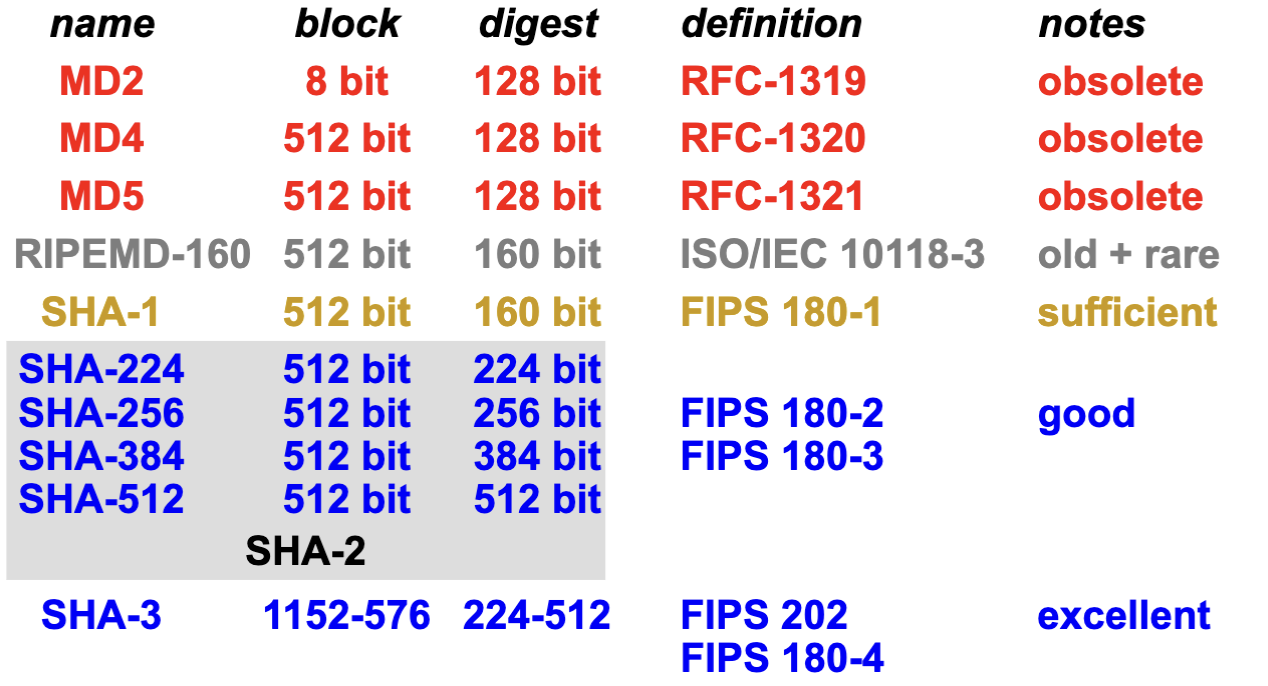
\includegraphics[width=0.5\linewidth]{Images/Cryptography/crypto_hash_functions.png}
    \caption{Cryptographic hash functions}
\end{figure}

\begin{center}
    \subsubsection*{The Algorithm}
\end{center}
Usually hash functions calculate digests through a chained process:
\begin{itemize}
    \item Split the message $M$ into $N$ blocks.
    \[
        M = M_1 || M_2 || \dots || M_N
    \]
    \item Iteratively apply a base function $f$ to each block.
    \[
        V_k = f(V_{k-1}, M_k) \quad \text{for} \quad k=1,2,\dots,N
    \]
    \[  
        \text{where} \quad V_0 = IV
    \]
    \item The final digest is the last value of the iteration $V_N$.
\end{itemize}

\begin{figure}[H]
    \centering
    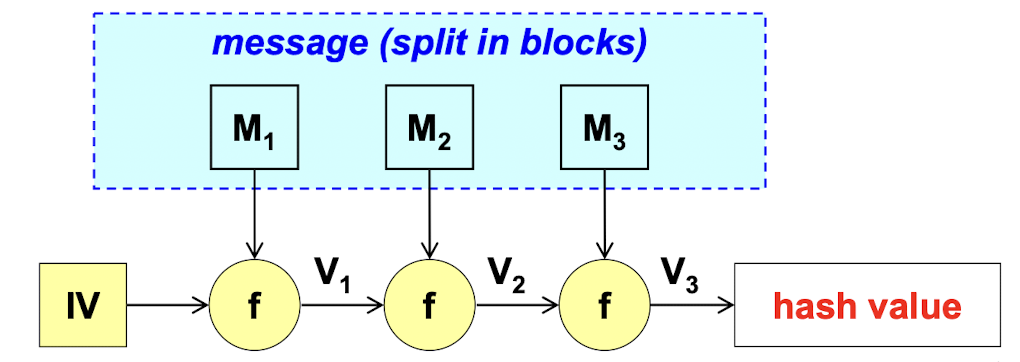
\includegraphics[width=0.5\linewidth]{Images/Cryptography/hash_f.png}
    \caption{Hash function process}
\end{figure}

\subsubsection*{Padding in Cryptographic Hash Functions}
Each function defines its own padding method.

For example, the \textbf{SHA-1} function has 512-bit blocks and uses the following padding:
\begin{itemize}
    \item Block size $B = 512$ bits and fragment (if the message length is not a multiple of 512 bits) size $L (< B)$ bits.
    \item Append a bit with value 1, followed by $K$ bits with value 0, where $K = B - L - 64$.
    \item The last 64 bits are the length of the original message.
\end{itemize}


\begin{tcolorbox}[colback=red!10!white, colframe=red!70!black, coltitle=white, title=Beware]
SHA-2 and SHA-3 are families of cryptographic hash functions. You must always specify the exact algorithm (SHA-256, SHA-512, etc.).
\end{tcolorbox}

\subsubsection*{SHA-2 Family}
\begin{center}
    (Secure Hash Algorithm 2)
\end{center}
SHA-2 is a family of cryptographic hash functions that includes SHA-224, SHA-256, SHA-384, SHA-512. The SHA-256 and SHA-512 algorithms are the most commonly used. As a quick fix after the SHA-1 attack, the SHA-2 family was developed by making the digest size larger.

SHA-224/-384 are the truncation of SHA-256/-512. 

\subsection{Digest Length}
The length of the digest is important because it determines the probability of a collision \newline (= \textcolor{Blue}{Aliasing}). 

If the algorithm is well-designed, and generates a digest of $N$ bits, \\ the probability of aliasing is:
\[
    P_A \propto \frac{1}{2^{N}}
\]
\dots thus, digests with many bits are required to avoid aliasing.

\subsection{The Birthday Paradox}
\begin{center}
    (Collision Probability, basic problem of hashing)
\end{center}

\begin{multicols}{2}
    The birthday paradox is a probability problem that asks how many people need to be in a room for the probability of two people sharing the same birthday to be greater than 50\%. The same concept applies to hash functions: the probability of two different messages having the same hash is higher than expected.

    \vspace{0.5cm}

    \begin{center}
        Reference Appendix A for the Birthday Attack.
    \end{center}

\columnbreak

    \begin{figure}[H]
        \centering
        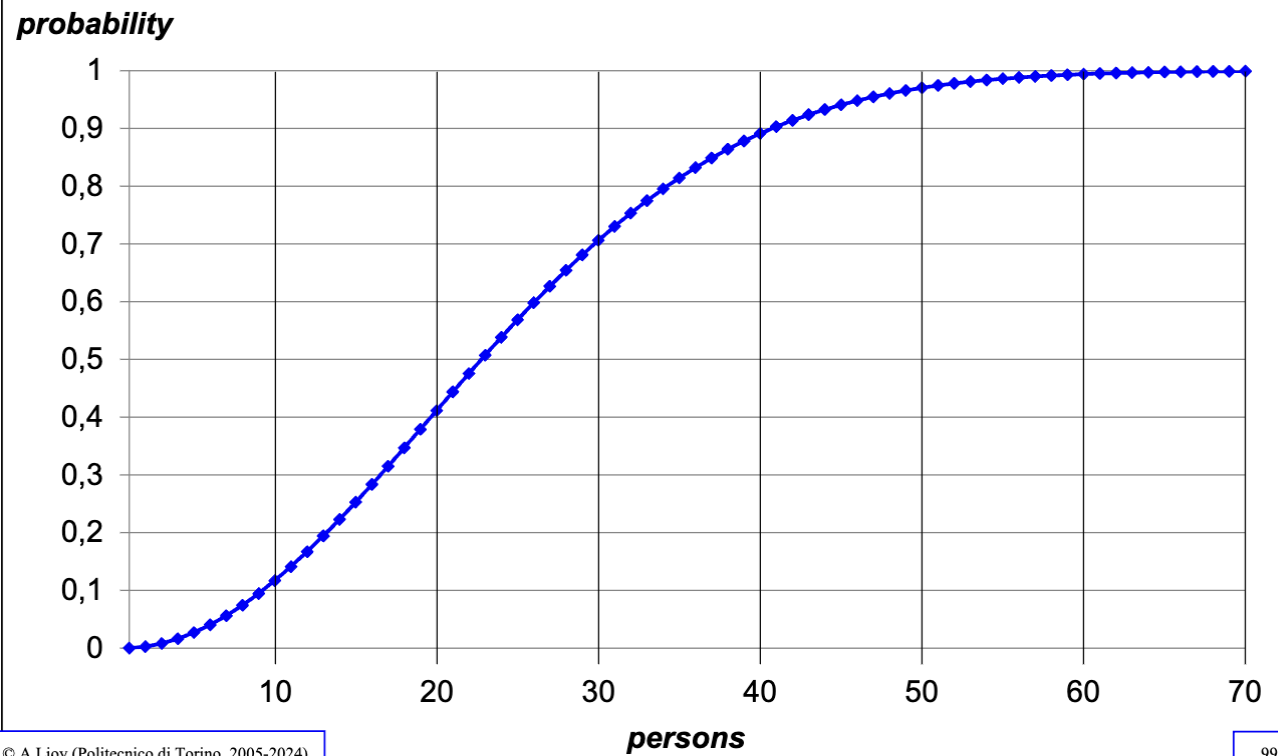
\includegraphics[width=\linewidth]{Images/Cryptography/bd_paradox.png}
        \caption{Birthday Paradox}
    \end{figure}
\end{multicols}



    \textbf{An $N$-bit hash function is considered insecure when more than $2^{N/2}$ digests are generated, because the probability to have two messages with the same digests is greater than 50\%. }

\textcolor{red}{Be aware:} A cryptosystem is balanced when the encryption and digest algorithms have the same resistance to attacks. SHA-256 and SHA-512 have been designed for use respectively with AES-128 and AES-256.

\begin{tcolorbox}[colback=red!10!white, colframe=red!70!black, coltitle=white, title=Beware]
    A system is only as secure as its weakest link.
\end{tcolorbox}

\subsubsection*{SHA-3 Family}
\begin{center}
    (Secure Hash Algorithm 3, named Keccak (pronounce: \textit{catch-ack}))
\end{center}
The SHA-3 family was developed as a backup to SHA-2 in case of a successful attack. The design of SHA-3 is completely different from that of SHA-2 and SHA-1.

\vspace{0.5cm}

\noindent Key features:
\begin{itemize}
    \item Elegant design.
    \item Run well on many computing devices.
    \item Higher performance in hardware implementations than SHA-2.
\end{itemize}

\begin{figure}[H]
    \centering
    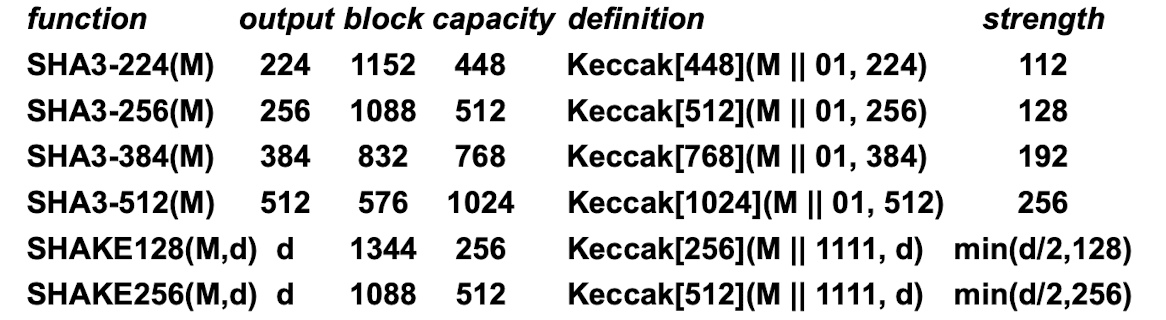
\includegraphics[width=0.5\linewidth]{Images/Cryptography/sha_3.png}
    \caption{SHA-3 family}
\end{figure}

\vspace{0.5cm}

And more (NIST SP: 800-185) SHA-3 family includes:
\begin{itemize}
    \item cSHAKE128, cSHAKE256: Customizable domain parameters.
    \item KMAC128, KMAC256: Keyed digest functions.
    \item TupleHash: Hash of a tuple, where sequence matters.
    \item ParallelHash: Fast hashing for multicore processors.
\end{itemize}

\section{Key Derivation Functions}
\begin{center}
    (KDF)
\end{center}
A cryptographic key must be random (each bit has a 50\% probability of being 0 or 1), but users typically choose passwords (or better, \textbf{passphrases}) guessable and not random. So the KDF is used to derive a key from a passphrase.

Main elements of a Key Derivation Function:
\[
    \text{KDF (P, S, I)} = \text{DerivedKey}
\]

\begin{itemize}
    \item P: Passphrase (e.g. password).
    \item S: Salt, to make K difficult to guess given P.
    \item I: how many times (Iterations) the function is applied (to slow down the computation and make life complex for attackers).
\end{itemize}

\vspace{0.2cm}

Some KDF based upon cryptographic hash functions:
\begin{itemize}
    \item PBKDF2 (Password-Based Key Derivation Function 2, RFC-2898).
    \begin{itemize}
        \item Uses SHA-1, $|S| \ge 64$, $|I| \ge 1000$.
    \end{itemize}
    \item HKDF (HMAC-based Extract-and-Expand Key Derivation Function, RFC-5869).
\end{itemize}

\subsection{Password-Based Key Derivation Function 2}
\begin{center}
    (PBKDF2, RFC-8018)
\end{center}

Main features:
\begin{itemize}
    \item Replaces PBKDF1, due to key length limitations ($\le 160$ bits).
\end{itemize}
Main elements to compute the derived key (DK):
\[
    \text{DK} = \text{PBKDF2 (PRF, PWD, Salt, C, dkLen)}
\]
\begin{itemize}
    \item PRF: Pseudo-Random Function with output length hLen(e.g. a keyed HMAC = HMAC-SHA-1).
    \item PWD: Password.
    \item Salt: Random value.
    \item C: Number of iterations desired.
    \item dkLen: Desired length of the derived key.
\end{itemize}

The Derived Key (DK) is constructed by concatenating components $T_1, T_2, \dots, T_{\lceil dkLen/hLen \rceil}$\footnote{$\lceil dkLen / hLen \rceil$  determines the number of components needed to reach or exceed the target key length.}, where each $|T_i| = hLen$.

\subsubsection*{PBKDF2 Parameters and Applications}
In WPA2 (Wi-Fi Protected Access 2), PBKDF2 is a core part of the 4-Way Handshake process. It is used to derive cryptographic keys securely from the Wi-Fi password to ensure encryption and integrity.
\[
    \text{(WPA2) DK = PBKDF2 (HMAC-SHA1, PSK, SSID, 4096, 256)}
\]

\clearpage
\section{Integrity, Authentication and Reliability Messages}
The following codes are sent with the message to ensure its integrity, authentication, and reliability, respectively:
\begin{itemize}
    \item MIC (Message Integrity Code): Computed using some data and a MIC function (can be a cryptographic hash function) to provide integrity (simil checksum). \textcolor{Blue}{Integrity}
    \item MAC (Message Authentication Code): Computed using a shared key, some data, and a MAC function (can be a cryptographic hash function, would be a keyed-digest). \textcolor{Blue}{Integrity and Authentication}
    \item MID (Message IDentification): A unique identifier to ensure the message is not duplicated (partially\footnote{Attackers can still forge messages based on the weaknesses of an identifier (management and synchronization.)} avoid replay attacks). \textcolor{Blue}{Reliability}
\end{itemize}

\begin{tcolorbox}[colback=red!10!white, colframe=red!70!black, coltitle=white, title=Beware]
    The added message should be encrypted; otherwise, a man-in-the-middle (MITM) attacker could modify both the hash and the message on-the-fly, bypassing integrity checks.
\end{tcolorbox}

\section{Keyed-Digest}
\begin{center}
    Possible implementation of a MAC.

    Authentication + Integrity.
\end{center}
\textcolor{Red}{No confidentiality!! The key has not this purpose in this mechanism.}

\hfill

A keyed-digest is obtained by applying a hash function to the message concatenated with a shared secret key. 
\begin{itemize}
    \item The sender sends the message and the keyed-digest to the receiver. 
    \item The receiver computes a keyed-digest of the same data (using the same shared key). 
    \item \textcolor{Blue}{Conclusion to say: }If the two digests match, the message is considered authentic (because used the same shared key) and integral (data not altered).

\end{itemize}
\begin{tcolorbox}[colback=red!10!white, colframe=red!70!black, coltitle=white, title=Beware]
If the check fails, we don't know if the message was altered or if the key was wrong. So the message and the keyed-digest must be discarded.
\end{tcolorbox}

\begin{multicols}{2}
    \raggedcolumns
    Advantages:
    \begin{itemize}
        \item Only one operation (hash).
        \item Few additional data (little overhead).
        \item Authentication + Integrity.
    \end{itemize}
\columnbreak

\begin{figure}[H]
    \centering
    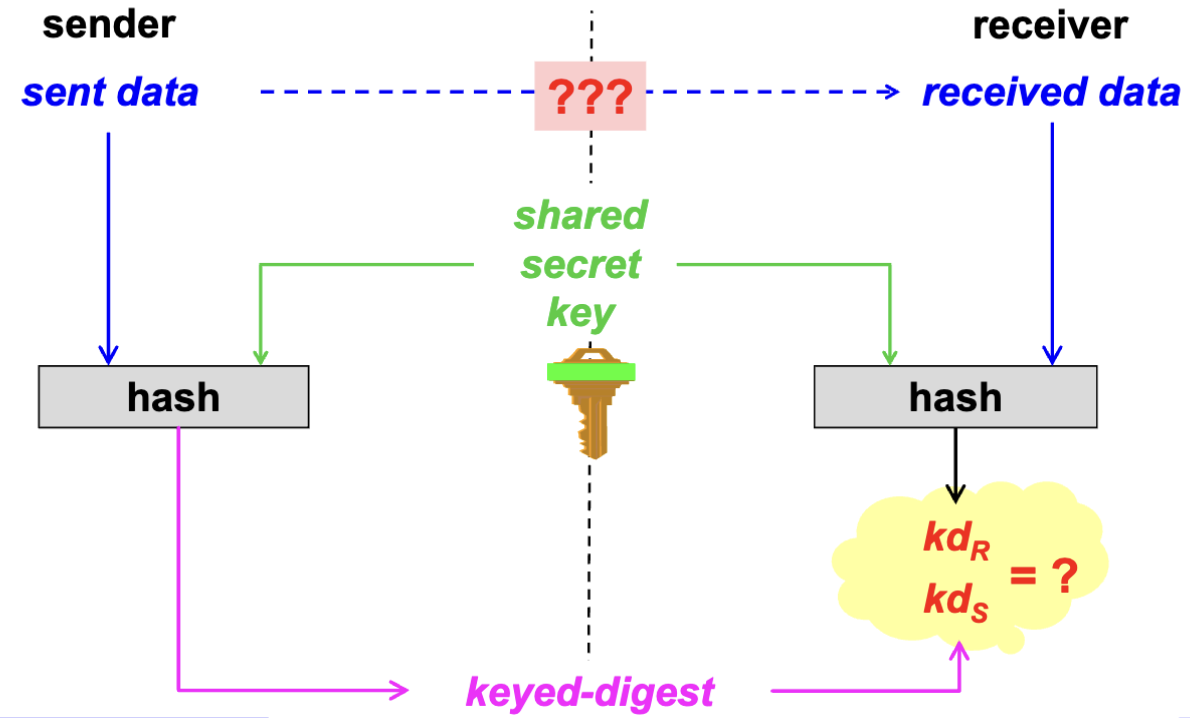
\includegraphics[width=\linewidth]{Images/Cryptography/keyed_digest.png}
    \caption{Keyed-Digest process}
\end{figure}
\end{multicols}

\subsection{Hash-based Message Authentication Code}
\begin{center}
    (HMAC) - RFC-2104 (also FIPS-198) - The only secure standard available.
    \\ Key-based method used to verify both the integrity and authenticity of a message  M .
\end{center}

\[
\text{HMAC-H} = \text{H}\big((K' \oplus \text{opad}) \, \| \, \text{H}((K' \oplus \text{ipad}) \, \| \, M)\big)
\]

\begin{itemize}
    \item H: Hash function (e.g. SHA-256).
    \item M: Message.
    \item K: The original secret key shared between two parties.
    \begin{itemize}
        \item $K' = H(K)$\quad if $|K| > B$.
        \item $K' = K$\quad\ \ \quad if $|K| \le B$.
    \end{itemize}
    \item K': The block-sized key derived from  K.
    \begin{itemize}
        \item 0-padded up to $B$ bytes\quad if $|K'| < B$.
    \end{itemize}
    \item ipad: Inner padding (0x36 repeated B times).
    \item opad: Outer padding (0x5C repeated B times).
\end{itemize}


\subsection{CBC-MAC}
\begin{center}
    (Cipher Block Chaining Message Authentication Code)
\end{center}
\textcolor{Red}{No for confidentiality!! No encryption of data.}

Main features:
\begin{itemize}
    \item Exploits a block-oriented symmetric encryption algorithm.
    \item CBC mod with null IV.
    \item Takes as MAC the last encrypted block.
\end{itemize}

\begin{center}
    \textbf{The Algorithm}
\end{center}
The message $M$ is divided into $N$ blocks $M_1, M_2, \dots, M_N$.
\begin{itemize}
    \item $V_0 = IV = 0$.
    \item $V_i = enc(V_{i-1} \oplus M_i, K)$ \quad \quad for ($i=1,2,\dots,N$).
    \item The MAC (aka CBC-MAC) is the last block $V_N$.
\end{itemize}

\subsubsection*{CBC-MAC Insecurity}
Reasons:
\begin{itemize}
    \item Secure only for fixed length messages (for other cases use CMAC or OMAC).
\end{itemize}
Possible attack against variable-length messages:
    \begin{itemize}
        \item If you have a CBC-MAC tag $t$ for a message $M$ and a tag $t'$ for another message $M'$, an attacker can construct a new message $M''$ such that the tag for $M''$ is valid without knowing the key $K$ (forgery attack).
        
\end{itemize}
\begin{center}
    Operational proof
\end{center}
    \begin{itemize}
        \item If I create a new message $M''$ as follows:
        \[
            M'' = M \, || \, (M'_1 \oplus t) \, || \, M'_2 \, || \, \dots \, || \, M'_N
        \]
        \begin{itemize}
            \item $M'_1 \oplus t$ modifies the first block of M' using the previous tag t to “cancel out” contributions.
        \end{itemize} 
        \[
            t'' = \text{CBC-MAC}(M'', K) = t'
        \]
        \item The resulting CBC-MAC tag for $M''$ ends up being $t'$, the tag of $M'$, effectively forging the message without knowing the key.
    \end{itemize}

\section*{Performances of Cryptographic Algorithms}
On large data, the computational effort of the cryptographic algorithms is:
\begin{figure}[H]
    \centering
    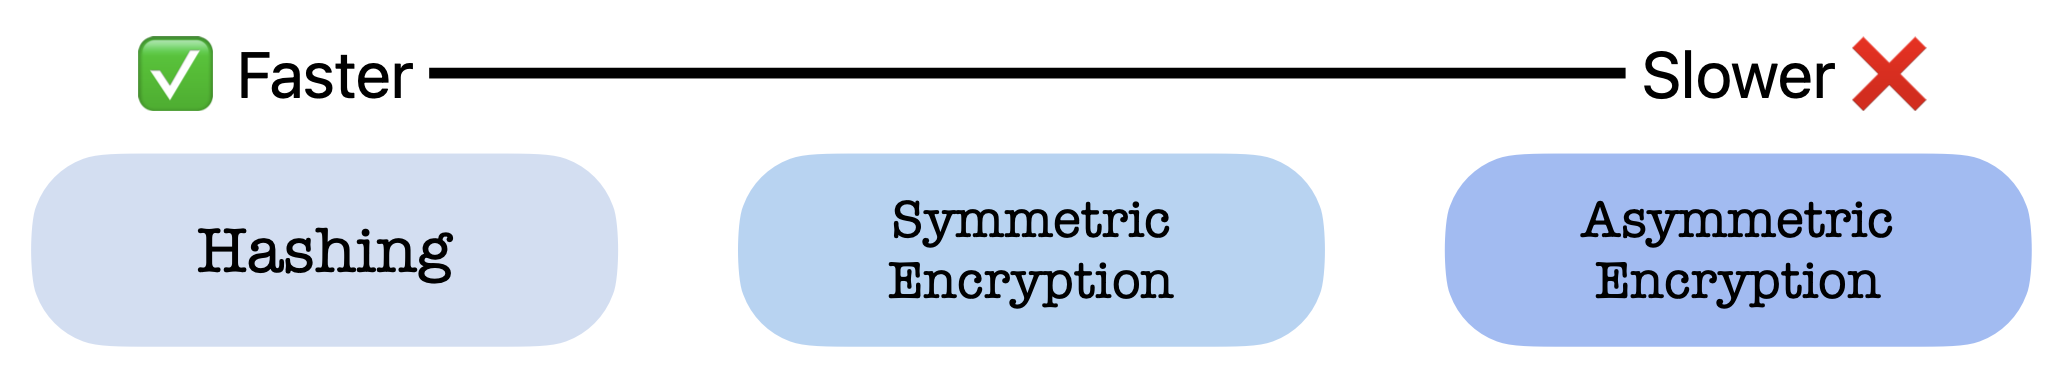
\includegraphics[width=0.7\linewidth]{Images/Cryptography/velocity.png}
    \caption{Hashing, Symmetric and Asymmetric Cryptography - Computational Effort}
\end{figure}

\clearpage 
\section{Integrity and Secrecy of Data}
\begin{center}
    (Confidentiality, Integrity and Authenticity)
\end{center}
We obtain:
\begin{itemize}
    \item Secrecy (confidentiality) from encryption with a key $K_1$.
    \item Authenticity, and integrity, from a MAC with a key $K_2$.
\end{itemize}

\hfill 

\begin{center}
    \textbf{Modalities}
\end{center}

    \begin{multicols}{2}

        \subsection*{Authenticate and Encrypt}
    \begin{center}
        A\&E
    \end{center}
    \[
        enc(K_1, M) \, || \, \text{MAC}(K_2, M)
    \]
    Key points:
    \begin{itemize}
        \item May leak info about the plaintext.
        \item Used by SSH.
        \item You will know if the message is corrupted at the end of the decryption.
        \item Insecure unless performed in a single step.
    \end{itemize}
\columnbreak

    \subsection*{Authenticate then Encrypt}
    \begin{center}
        AtE
    \end{center}
    \[
        enc(K_1, M \, || \, \text{MAC}(K_2, M))
    \]
    Key points:
    \begin{itemize}
        \item No info leakage.
        \item Used by SSL/TLS.
        \item Secure only with CBC or stream encryption.
    \end{itemize}
\end{multicols}

\begin{center}
    \subsection*{Encrypt then Authenticate}
    \begin{center}
        EtA \\ Best solution.
    \end{center}
    \[
        enc(K_1, M) \, || \, \text{MAC}(K_2, enc(K_1, M))
    \]
\end{center}

Key points:
\begin{itemize}
    \item Can avoid decryption if MAC is wrong
    \item Used by IPsec.
    \item The most secure mode, but beware of implementation errors (e.g., always include the  IV  and algorithms in the MAC).
\end{itemize}

\begin{tcolorbox}[colback=red!10!white, colframe=red!70!black, coltitle=white, title=Beware]
    Improper combination of secure algorithms may lead to an insecure result !
\end{tcolorbox}
A modern solution to that is Authenticated Encryption (AE) that combines encryption and authentication in a single operation.

\subsection{Authenticated Encryption}
\begin{center}
    (AE)
\end{center}
A single operation for privacy and authentication/integrity.

Key features:
\begin{itemize}
    \item Just one key and one algorithm.
    \item Better speed.
    \item Less error likelihood in combining the two functions.
\end{itemize}

\subsubsection{Infinite Garble Extension}
\begin{center}
    (IGE - for Authenticated Encryption)
\end{center}
A mode of operation for block ciphers that provides both confidentiality and authenticity.

\[
    C_i = P_{i-1} \oplus enc(K_, C_{i-1} \oplus P_i) \quad \text{for} \quad i=1,2,\dots,N \text{ blocks}
\]
\[
    C_1 = IV \oplus enc(K_, P_1 \oplus enc (K', IV))
\]

\begin{figure}[H]
    \centering
    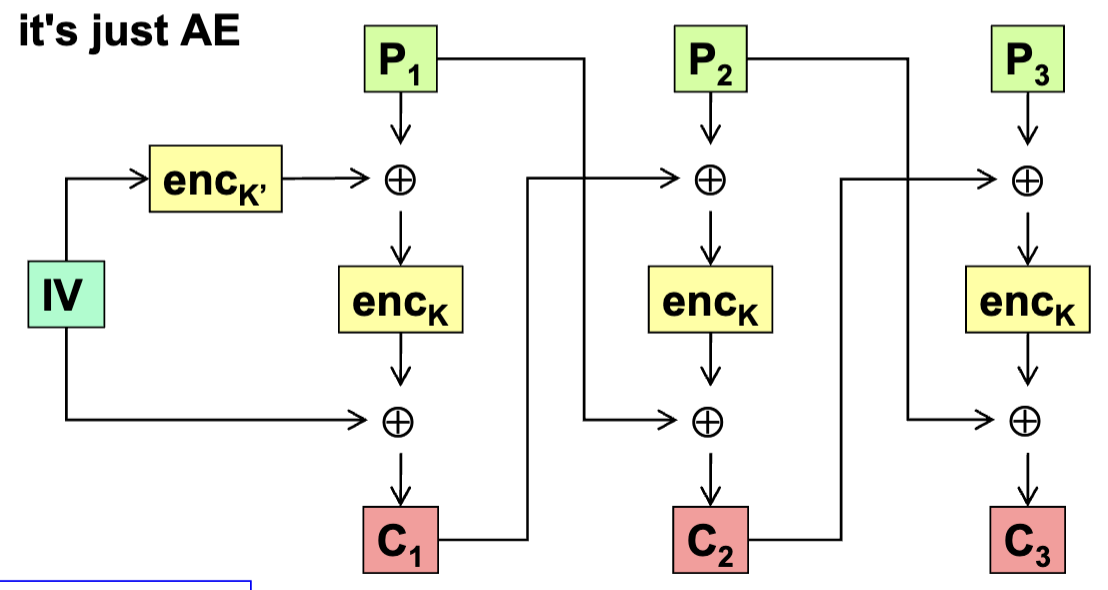
\includegraphics[width=0.5\linewidth]{Images/Cryptography/AE.png}
    \caption{Infinite Garble Extension process}
\end{figure}

\clearpage
\subsection{Authenticated Encryption with Associated Data Schema}
\begin{center}
    (AEAD - Authenticated Encryption with Associated Data)
\end{center}
\begin{tcolorbox}[colback=red!10!white, colframe=red!70!black, coltitle=white, title=Beware]
    AEAD is not a single algorithm but a cryptographic scheme that combines encryption and authentication. 
\end{tcolorbox}
Due to its Authenticated Encryption (AE) nature, it performs both encryption (confidentiality) and authentication (integrity and authenticity) in a single operation. AEAD ensures that any modification to the ciphertext or associated data is detectable.

\begin{figure}[H]
    \centering
    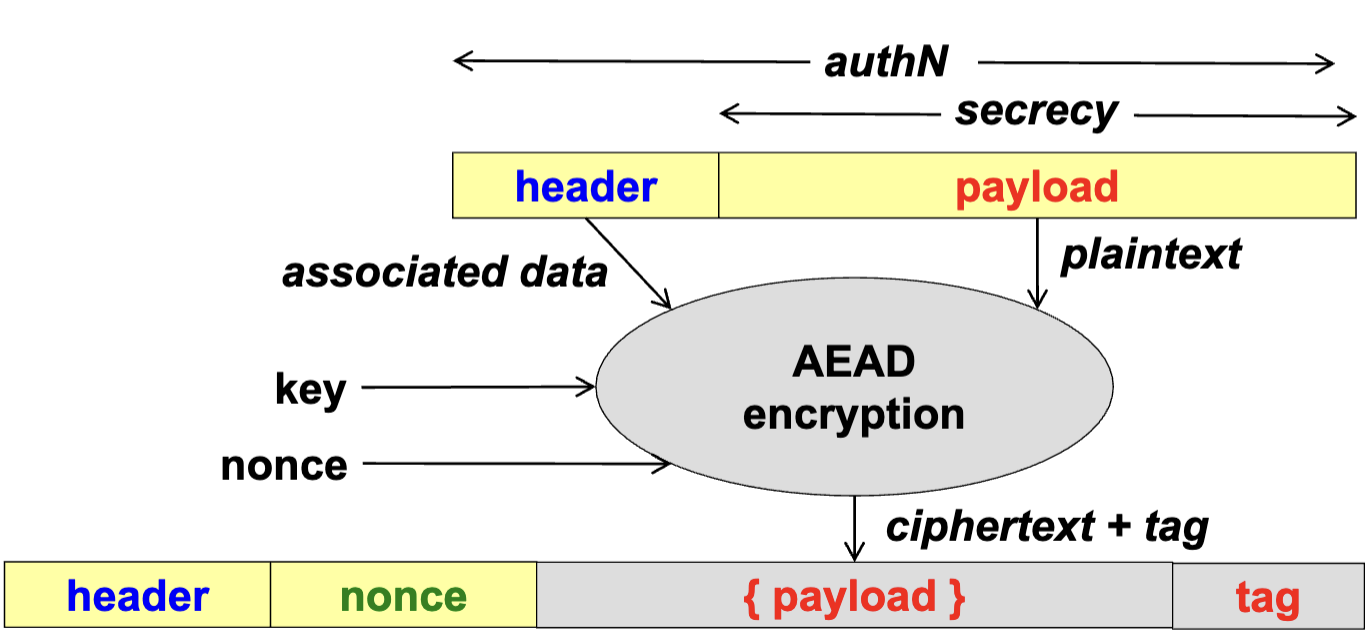
\includegraphics[width=0.6\linewidth]{Images/Cryptography/aead.png}
    \caption{AEAD scheme}
\end{figure}

\subsection{AE Standards}
Many are issued by NIST and IETF:
\begin{itemize}
    \item GCM (Galois/Counter Mode).
    \item CCM (CTR mode with CBC-MAC): off-line double-pass, the slowest one.
    \item EAX (Encrypt-then-Authenticate-then-Encrypt with X translation = CTR + OMAC): on-line double-pass AEAD. Slow but small (uses just the encryption block) so very good for constrained systems.
    \item OCB (Offset Codebook Mode): the fastest one, on-line single-pass AEAD. GPL patented so scarcely used, now free but for military uses.
    \item AESKW (AES Key Wrap).
    \item Encrypt-then-MAC (EtM).
\end{itemize}
\begin{tcolorbox}[colback=blue!10!white, colframe=blue!50!white]
Double-pass is 2x slower than single-pass (in software).
\end{tcolorbox}

\clearpage

\subsubsection{Galois/Counter Mode as AEAD}
\begin{center}
    GCM as an example of AEAD. \\ Defined for encryption algorithms with 128-bit block size.
\end{center}
Is the most popular, on-line single-pass AEAD, parallelizable.
\[
    \text{(C, T)} = \text{GCM\_enc}(K, IV, A, P)
\]
\begin{itemize}
    \item Outputs:
    \begin{itemize}
        \item $C$: Ciphertext, with same size as $P$.
        \item $T$: Authentication Tag, with size $[1, ..., 2^{128}]$ bits.
    \end{itemize}
    \item $IV$: Initialization Vector, with size $[1, ..., 2^{64}]$ bits (96 bits is common).
    \item $P$: Plaintext, with size $[1, ..., 2^{39}-256]$ bits.
    \item $A$: Associated Data, not encrypted but authenticated, with size $[1, ..., 2^{64}]$ bits.
    \item $K$: Key.
\end{itemize}

If the authentication is OK then it is possible to decrypt the message.
\[
    \text{P} = \text{GCM\_dec}(K, IV, A, C, T)
\]
\begin{tcolorbox}[colback=blue!10!white, colframe=blue!50!white, title=Output of decryption]
    If the authentication is OK then the output is the plaintext, otherwise a special value FAIL is returned.
\end{tcolorbox}
Is present in openssl:
\begin{itemize}
    \item For encryption: ciphertext+authentication-tag generation.
    \item For decryption: first computes the authentication tag and then decrypts the ciphertext if the tag is OK (matches the one in input).
    \item Fast on Intel architecture using AES-NI for encryption and PCLMULQDQ for the tag.
\end{itemize}

\subsubsection{CTR mode with CBC-MAC as AEAD}
\begin{center}
    CCM as an example of AEAD. \\ Defined for encryption algorithms with 128-bit block size.
\end{center}
First an authentication tag of the plaintext and associated data is calculated using CBC-MAC. Then the plaintext and associated data are encrypted using CTR mode. Then the plaintext and the tag are (separately) encrypted using CTR mode.

\subsubsection{AES Key Wrap}
\begin{center}
    AESKW - RFC-3394 \\ Only for keys, not data.
\end{center}
Assumptions:
\begin{itemize}
    \item The protocol encrypts/decrypts a key for storage/transmission.
    \item The key is a multiple of 64 bits.
    \item Generates also a 64-bit authentication tag.
\end{itemize}

\begin{center}
    \textbf{The Operations}
\end{center}
\begin{enumerate}
    \item KEK (Key Encryption Key) is the key used to encrypt/decrypt the key.
    \item CEK (Content Encryption Key) is the key to be encrypted/decrypted.
    \item {CEK} + tag = AESKW\_enc(KEK, CEK).
    \item CEK (or FAIL) = AESKW\_dec(KEK, {CEK} + tag).
\end{enumerate}
This protocol, unlike normal AE algorithms, is simple (e.g. no RNG as in GCM needed, or no asymmetric encryption) and supports in-place encryption/decryption.

\subsubsection{ASCON}
\begin{center}
    Used for encryption, AEAD, and hashing.
\end{center}
NOT to replace AES or SHA3, but to be used in constrained (lightweight) environments (e.g. IoT).
\begin{center}
    \textbf{For AEAD}
\end{center}

\begin{table}[H]
    \centering
    \begin{tabular}{lccccccc}
        \toprule
        \textbf{} & \textbf{key} & \textbf{nonce} & \textbf{tag} & \textbf{rate} & \textbf{capacity} & \textbf{pa} & \textbf{pb} \\
        \midrule
        ASCON-128  & 128 & 128 & 128 & 64  & 256 & 12 & 6 \\
        ASCON-128a & 128 & 128 & 128 & 128 & 192 & 12 & 8 \\
        \bottomrule
    \end{tabular}
\end{table}

\begin{center}
    \textbf{For Hashing}
\end{center}
\begin{table}[H]
    \centering
    \begin{tabular}{lcccccc}
        \toprule
        \textbf{} & \textbf{output} & \textbf{rate} & \textbf{capacity} & \textbf{pa} & \textbf{pb} \\
        \midrule
        ASCON-hash  & 256       & 64  & 256 & 12 & 12 \\
        ASCON-xof   & arbitrary & 64  & 256 & 12 & 12 \\
        ASCON-hasha & 256       & 64  & 256 & 12 & 8  \\
        ASCON-xofa  & arbitrary & 64  & 256 & 12 & 8  \\
        \bottomrule
    \end{tabular}
\end{table}
\begin{tcolorbox}[colback=blue!10!white, colframe=blue!50!white]
pa and pb are the number of rounds for the permutation and the number of rounds for the key schedule, respectively. The higher the number of rounds, the higher the security but also the computational effort.
\end{tcolorbox}

\subsection{AE Applications}
Here are listed some applications of AE:
\begin{itemize}
    \item TLS-1.3 (Transport Layer Security) uses GCM and CCM.
    \item 802.11i (wi-fi) uses CCM.
    \item ZigBee uses CCM* (a variant of CCM, = CCM + auth-only + enc-only).
\end{itemize}

\section{Authentication by Digest and Asymmetric Encryption}
\begin{center}
    (Real implementation of Digital Signatures)
\end{center}
The sender sends the message digest encrypted with the private key. The receiver decrypts the digest with the public key of the sender and compares it with the digest of the message. If they match, the message is authentic.
\begin{verbatim}
    Sender: 
        signedDigest = enc(hash(Message), S.SecretKey)

    Sender > Receiver:
        Message, signedDigest 

    Verifier:
        digest = dec(signedDigest, S.PublicKey)
        hash(Message) == digest ? OK : ALARM
\end{verbatim}

Those who know the public key can compare the transmitted digest with the digest calculated on the received data. It's the basis of digital signatures !! 


\clearpage

\subsection{Digital Signature}
\begin{center}
    The technical basis for digital signatures.

    Authentication + Integrity + Non-repudiation.
\end{center}
\begin{center}
    \textbf{The Algorithm}
\end{center}
The digital signature process involves creating a secure and verifiable way to ensure the authenticity, integrity, and non-repudiation of digital data. The process is as follows:
\begin{enumerate}
    \item The sender generates pair of cryptographic keys (PublicKey and SecretKey).
    \item A cryptographic \textbf{hashing} algorithm is applied to the data (message or file) to obtain a hash value.
    \item The private key is used to \textbf{encrypt} this hash value, producing the digital signature (signed hash).
    \item The signed data (original data + digital signature) is sent to the receiver.
    \item The receiver uses the sender's public key to decrypt the signature, in order to obtain the digest to verify.
    \item The receiver applies the same hashing algorithm to the received message/data.
    \item If the decrypted hash matches the hash computed locally, the digital signature is valid. This verifies:
    \begin{itemize}
        \item Authenticity: The message came from the expected sender.
        \item Integrity: The data has not been altered.
        \item Non-repudiation: The sender cannot deny having sent the message (due to the use of its own private key).
    \end{itemize}
\end{enumerate}
\begin{tcolorbox}[colback=red!10!white, colframe=red!70!black, coltitle=white, title=Beware]
In order to check the integrity of the message, the receiver must have the public key of the sender. The public key won't stay the same forever. It can be changed, so the verifier must have a way to know the new public key.
\end{tcolorbox}

\begin{figure}[H]
    \centering
    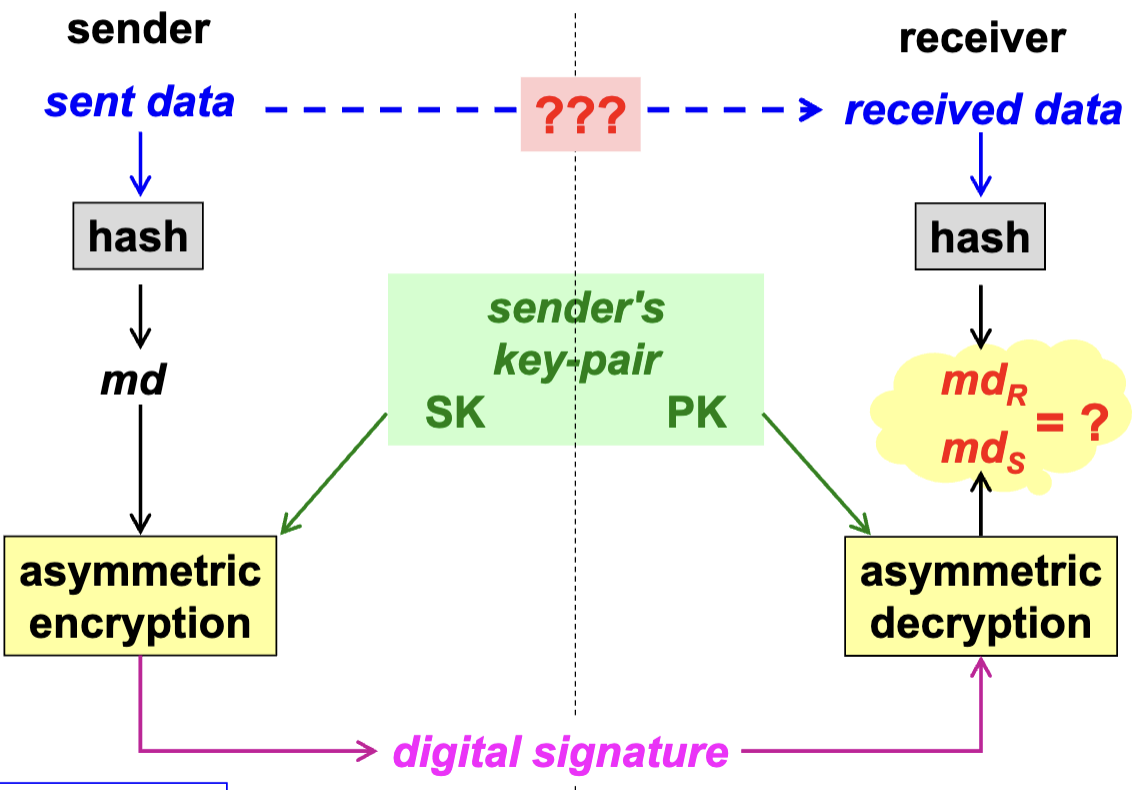
\includegraphics[width=0.4\linewidth]{Images/Cryptography/ds.png}
    \caption{Digital Signature transmission}
\end{figure}
\begin{tcolorbox}[colback=red!10!white, colframe=red!70!black, coltitle=white, title=For the Exam]
    The sender is sending the data + digital signature (encrypted hash of the message) to the receiver. 
    
    \vspace{0.2cm}
    
    Whether the manipulation happen in the data or in the digital signature, the receiver will detect it (and reject everything).
\end{tcolorbox}


\begin{center}
    \textbf{Signature Verification for Stored Data}
\end{center}

The mechanism seen above is valid also for storing data. The data is stored with the digital signature. When the data is read, the digital signature is decrypted and compared with the hash of the data. If they match, the data is authentic.
\begin{tcolorbox}[colback=blue!10!white, colframe=blue!50!white]
Once the data are signed, even if they are store in a public place, the verifier can verify the integrity of the data.
\end{tcolorbox}

\begin{figure}[H]
    \centering
    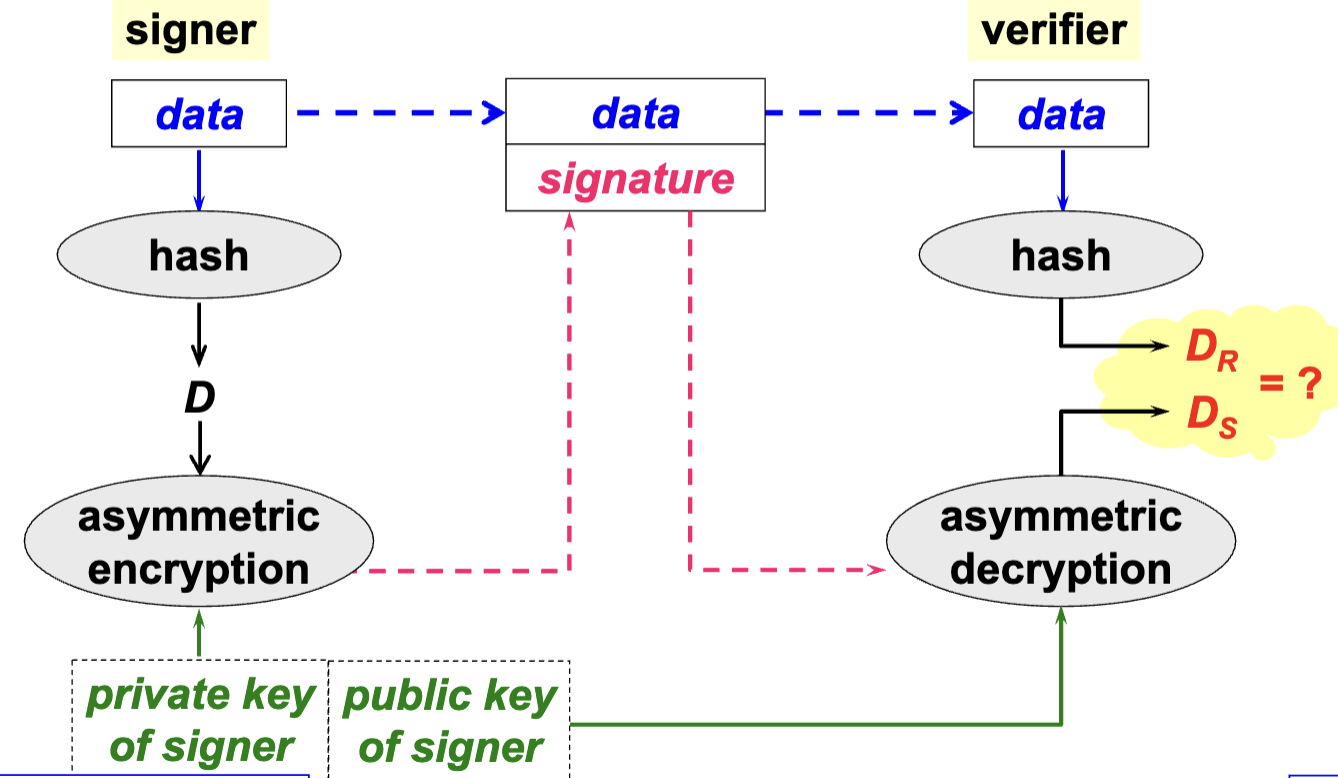
\includegraphics[width=0.6\linewidth]{Images/Cryptography/ds_storing.png}
    \caption{Digital Signature stored with the data}
\end{figure}

\subsubsection*{Digital Signature and Handwritten Signature}
\begin{multicols}{2}

    Digital signature: \\ Authentication + Integrity.
    \begin{itemize}
        \item Better because it is tightly linked to the data.
        \item Each user does not have a digital signature but a private key, which can be used to generate an infinite number of digital signatures (one for each document).
    \end{itemize}
    \columnbreak

    

    Handwritten signature: \\ Only Authentication.
    
\end{multicols}

\clearpage

\subsection{Authentication and Integrity Analysis}


\begin{multicols}{2}

    \textbf{The use of a shared secret for providing Authentication and Integrity (MAC)}:
    \begin{itemize}
        \item Useful only for the receiver.
        \item Cannot be used as a proof without disclosing the secret key.
        \item Does not provide non-repudiation.
    \end{itemize}
\columnbreak

\textbf{The use of asymmetric encryption for providing Authentication and Integrity (Digital Signature)}:
\begin{itemize}
    \item Applied only to the digest (because of the computational effort).
    \item Can be used as a formal proof-of-origin.
    \item Provides non repudiation.
\end{itemize}
\end{multicols}



\section{Public Key Infrastructure}
\begin{center}
    (PKI)
\end{center}
The PKI provides a framework for managing digital certificates and public-key encryption.

\subsection{Public Key Certificate}
\begin{center}
    Definition: \\ A data structure used to securely bind a public key to some attributes.
\end{center}

Typically, it binds a key to an identity, but other associations are possible too (e.g. IP address, domain name, etc.). The certificate is signed by a trusted third party, the Certificate Authority (CA), to ensure the authenticity of the binding. The certificate has a limited lifetime, after which it must be renewed. Can be revoked on request both by the user and the issuer.

\vspace{0.5cm}

Formats for public key certificates:
\begin{itemize}
\item X.509:
\begin{itemize}
\item v1: Initial version.
\item v2: Enhanced version introduced by ISO.
\item v3: Most commonly used version, combining ISO and IETF standards.
\end{itemize}
\item Non X.509:
\begin{itemize}
\item PGP (Pretty Good Privacy).
\item SPKI (Simple Public Key Infrastructure, IETF).
\end{itemize}
\item PKCS\#6 (Public Key Cryptography Standard \#6):
\begin{itemize}
\item RSA certificates, partially compatible with X.509.
\item Now considered obsolete.
\end{itemize}
\end{itemize}

\clearpage 
\subsubsection{X.509 Certificate}
\begin{center}
    The most common format for public key certificates.
\end{center}
\begin{center}
    \textbf{The Structure}
\end{center}

\begin{multicols}{2}

    \begin{itemize}
        \item Version: The version of the X.509 standard.
        \item Serial Number: A unique number assigned by the CA.
        \item Signature Algorithm: The algorithm used by the CA to sign the certificate.
        \item Issuer: The entity that issued the certificate.
        \item Validity: The period during which the certificate is valid.
        \item Subject: The entity to which the certificate is issued. Written with its Distinguished Name (DN).
        \item Subject Public Key Info: The public key of the subject.
        \item CA Signature: The digital signature of the CA.
    \end{itemize}

\columnbreak

    \begin{figure}[H]
        \centering
        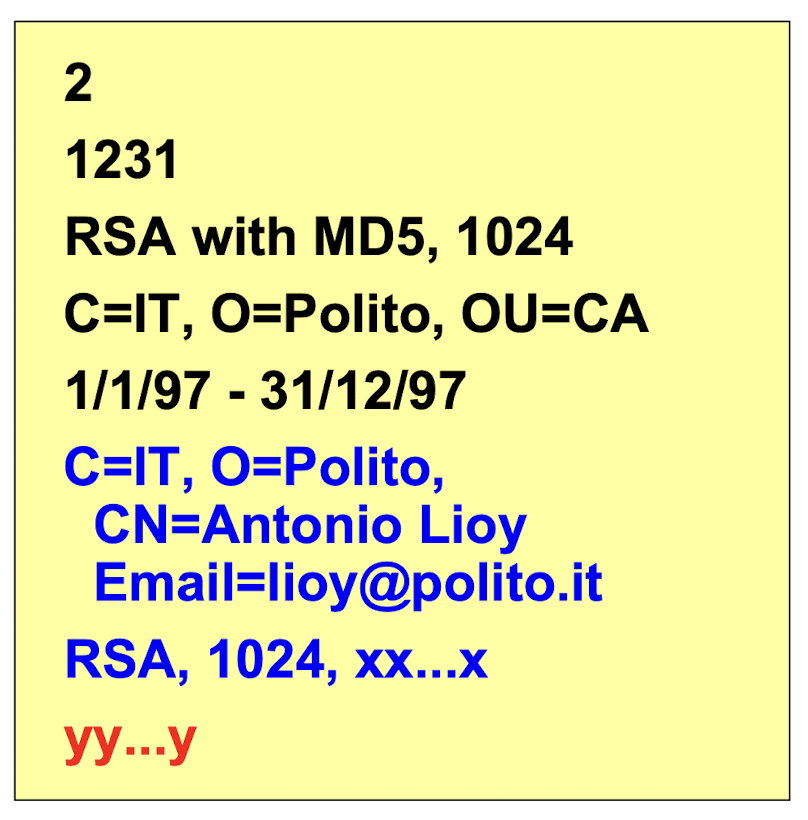
\includegraphics[width=\linewidth]{Images/Cryptography/x509.png}
        \caption{X.509 Certificate structure}
    \end{figure}
\end{multicols}

\subsection{Certificate Revocation}
Any certificate can be revoked before its expiration date:
\begin{itemize}
\item At the request of the owner (subject).
\item Unilaterally by the issuer (issuer).
\end{itemize}
When verifying a signature, the receiver must ensure that the certificate was valid at the time the signature was created. This \textbf{verification is responsibility of the receiver}, also referred to as the “Relying Party” (RP).

\subsubsection*{Revocation Mechanisms}
\begin{itemize}
    \item CRL (Certificate Revocation List):
    A list of revoked certificates published and signed by the Certificate Authority (CA). It provides information about the validity of certificates since their issuance.
    \item OCSP (Online Certificate Status Protocol);  
A real-time protocol used to check the revocation status of a certificate. The response is signed by the OCSP responder (server), and the validity of the certificate is verified at the time of the request.  
\end{itemize}

\clearpage

\subsubsection*{X.509 CRL Structure}

\begin{multicols}{2}

    \begin{itemize}
        \item Version: The version of the X.509 standard.
        \item Signature Algorithm: The algorithm used by the CA to sign the CRL.
        \item Issuer: The entity that issued the CRL.
        \item This Update: The date of the last update.
        \item User Certificate Revocation Date: The date of revocation.
        \item CA digital signature.
    \end{itemize}
\columnbreak

    \begin{figure}[H]
        \centering
        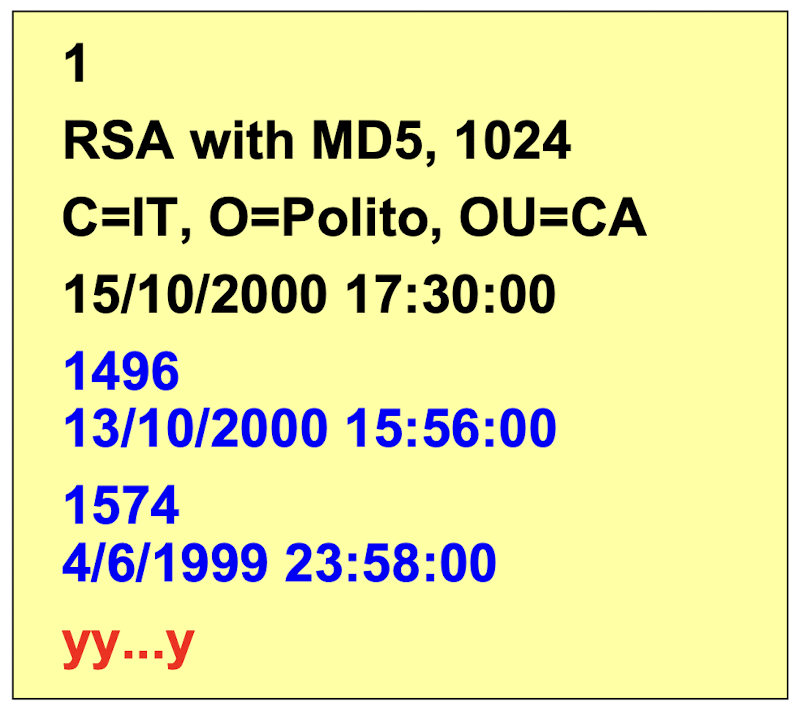
\includegraphics[width=\linewidth]{Images/Cryptography/x509_crl.png}
        \caption{X.509 CRL structure}
    \end{figure}
\end{multicols}

\subsection{Verification of a Signature/Certificate}

\begin{tcolorbox}[colback=blue!10!white, colframe=blue!50!white]
    It is necessary to have an infrastructure for the certification and distribution of public-key certificates, as well as for the dissemination of their respective revocation information.
\end{tcolorbox}

\begin{center}
    \textbf{The Process}
\end{center}
The verifies must:
\begin{enumerate}
    \item Check if the public key of the sender is valid (created within the validity period of the certificate) and the public key certificate was issued by a trusted CA.
    \item Decrypt the digital signature using the public key of the sender ($X$). The decrypted value represents the digest extracted from the signature.
    \item Calculate the hash of the data (message or file) using the same hash function as the signer.
    \item Compare the two digests: If they match, the signature is valid, confirming both the authenticity (the signature belongs to $X$) and the integrity (the data has not been altered).
    \item If the digests do not match, the signature is invalid, indicating either tampering with the data or an incorrect public key.
    \end{enumerate}
\begin{figure}[H]
    \centering
    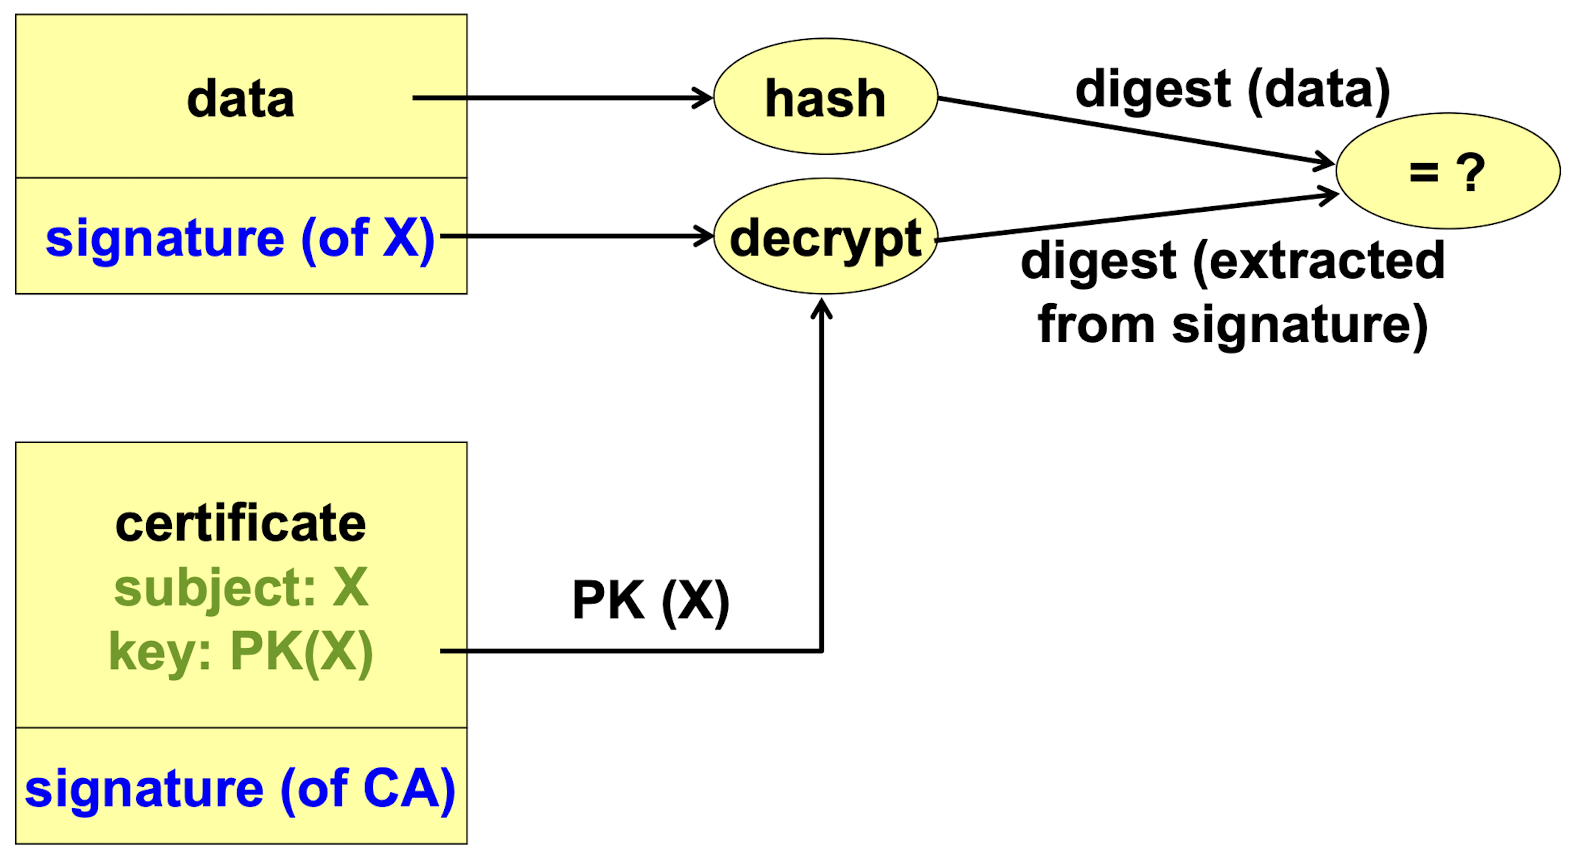
\includegraphics[width=0.5\linewidth]{Images/Cryptography/cert_verif.png}
    \caption{Verification process of a Signature/Certificate}
\end{figure}

\subsection{Certification Hierarchy}
\begin{center}
    (Chain of Trust)
\end{center}
The diagram \ref{fig:cert_hier} illustrates the Certification Hierarchy (also called the Chain of Trust) in a Public Key Infrastructure (PKI).

\hfill

Starting from the top:
\begin{enumerate}
    \item Top-Level Certification Authority (TLCA or Root CA): The highest level of the hierarchy, which issues certificates to intermediate CAs. It is the trusted entity that signs certificates for lower-level Certification Authorities (CAs). 
    \[
        \text{All trust starts here, and this CA is implicitly trusted in the PKI.}
    \]
    \item Intermediate Certification Authority (ICA): An entity that issues certificates to end entities (users, servers, etc.).
    \item Lower-Level (Local) CAs.
\end{enumerate}
\begin{tcolorbox}[colback=red!10!white, colframe=red!70!black, coltitle=white, title=Beware]
    Each CA at any level in the hierarchy signs certificates with its digital signature (ds). The signature is verified by the next higher-level CA in the hierarchy.
\end{tcolorbox}
\begin{figure}[H]
    \centering
    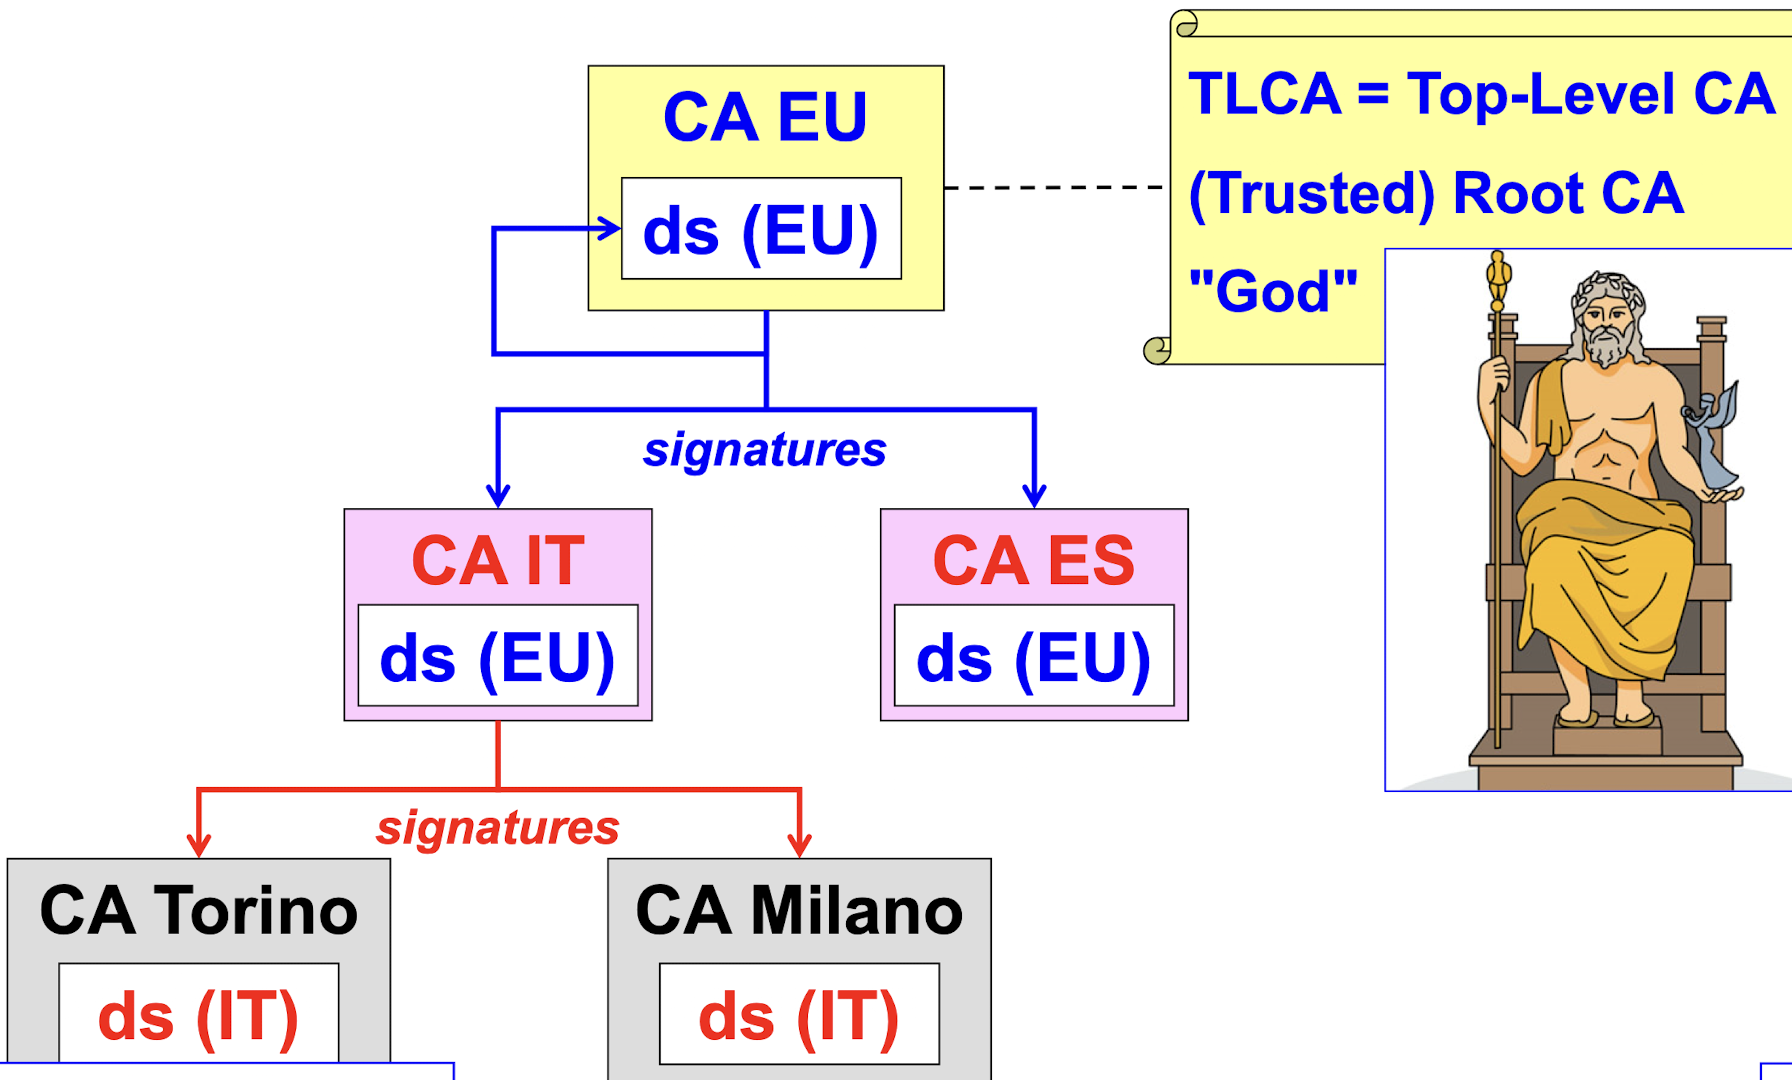
\includegraphics[width=0.5\linewidth]{Images/Cryptography/cert_hier.png}
    \caption{Example of Certification Hierarchy}
    \label{fig:cert_hier}
\end{figure}

\section{Commercial National Security Algorithm Suite}
\begin{center}
    CNSA Suite 2018
\end{center}
Includes the following algorithms:
\begin{itemize}
    \item Symmetric Encryption: AES-256 (Advanced Encryption Standard 256), with mode CTL (low bandwidth) or GCM (high bandwidth).
    \item Hashing: SHA-384 (Secure Hash Algorithm 512 truncated to 384 bits).
    \item Key Agreement: ECDH-384 (Elliptic Curve Diffie-Hellman) and ECMQV (Elliptic Curve Menezes-Qu-Vanstone).
    \item Digital Signature: ECDSA-384 (Elliptic Curve Digital Signature Algorithm).
    \item Elliptic Curve (EC): Curve P-384.
    \end{itemize}
    
    For legacy systems:
    \begin{itemize}
    \item Key Agreement: DH-3072 (Diffie-Hellman).
    \item Key Exchange and Digital Signature: RSA-3072 (Rivest-Shamir-Adleman).
    \end{itemize}
    
    \vspace{1cm}
    
    \begin{center}
    CNSA Suite 2022
    \end{center}
    
    Includes the following algorithms:
    \begin{itemize}
    \item Symmetric Encryption: AES-256 (Advanced Encryption Standard 256), with mode CTL (low bandwidth) or GCM (high bandwidth).
    \item Hashing: SHA-384 or SHA-512.
    \item Key Agreement: CRYSTALS-Kyber with level V parameters.
    \item Digital Signature: CRYSTALS-Dilithium with level V parameters.
    \item Digital Signature for Firmware and Software:
    \begin{itemize}
    \item All NIST SP 800-208 algorithms (LMS, XMSS).
    \item Suggested: LMS SHA-256/192.
    \end{itemize}
    \end{itemize}
%\chapter{Authentication Techniques, Protocols and Architectures}

\section*{Definitions}

\blockquote[RFC-4949 (Internet Security Glossary)]{
    The process of verifying a claim that a system entity or system source has a certain attribute value.
}

\vspace{0.3cm}

\blockquote[whatis.com]{The process of determining whether someone or something is who or what it is declared to be.}

\vspace{0.3cm}

\blockquote[NIST IR 7298]{Verifying the identity of a user, process, or device, often as a prerequisite to allowing access to resources in an information system.} 

\section{Authentication Factors}

\vspace{0.3cm}

\hrule


\begin{multicols}{3}
    \begin{center}
        \large{\textbf{Knowledge}}
    \end{center}
    
    \columnbreak
    \columnseprule=0.5pt

    \begin{center}
        \large{\textbf{Ownership}}
    \end{center}
    \columnbreak

    \begin{center}
        \large{\textbf{Inherence}}
    \end{center}
\end{multicols}

\begin{center}
    \repeatchar{20}{-} IS \repeatchar{20}{-}
\end{center}

\begin{multicols}{3}
    \begin{center}
    Something only the user knows (passwords, PINs, etc.)
\end{center}


    
    \columnbreak

    Something only the user has (smart cards, tokens, etc.)

    \vspace{0.1cm}

    Often called "Authenticators".
    \columnbreak

    Something only the user is (biometrics, etc.)


\end{multicols}

\begin{center}
    \repeatchar{10}{-} \textbf{Risks} \repeatchar{10}{-}
\end{center}


\begin{multicols}{3}
    Storage and demonstration/transmission.

    \columnbreak

    Authenticator itself, theft, cloning, unauthorized use.

    \columnbreak
Counterfeiting and privacy. Cannot be replaced when "compromised".

Use it only for local authentication! As mechanism to unlock a secret or a device.
    
\end{multicols}

Applications are not only for humans, but also for devices, services, etc.

\begin{tcolorbox}[colback=blue!10!white, colframe=blue!50!white, title=What about Authorization]
    Authentication and Authorization are two different things, but strictly related. Authentication leads to Authorization/Access Control.
\end{tcolorbox}

\section{Digital Authentication Model}
\begin{center}
    NIST SP 800-63B \\ Generic Architecture (Roles might be separated or collapsed together)
\end{center}

\noindent Digital authentication \textbf{entities:} 
\begin{itemize}
    \item Applicant: an entity that wants to obtain a credential (e.g., A new employee at a company).
    \item Credential Service Provider (CSP) (e.g., POLITO), which, for applicants, is responsible for:
    \begin{itemize}
        \item Identity Proofing: Verifying the applicant's claimed identity.
        \item Authenticator Enrollment: Issuing an authenticator (e.g., a password, hardware token, or biometric tool) that binds the applicant's identity to the credential.
        \item Storing attributes of the applicant's identity.
    \end{itemize}
    \item Claimant: An entity that asserts a claim of identity during an authentication process (e.g., a subscribed employee who asserts its identity in order to gain access).
    \item Subscriber: An entity whose identity has been verified by a Credential Service Provider (CSP) and who has been issued an authenticator (e.g., the new employee after successful verification and issuance of an authenticator, or the subscribed employee after logging in).
    \item Verifier: An entity that verifies the claimant's identity by executing the authentication protocol using the claimant's issued credentials.
\end{itemize}

\hfill

\begin{center}
    \textbf{The Algorithm}
\end{center}

The model has two entries: applicant and claimant. Below are the steps for each entry:

\begin{enumerate}
    \item The process begins with the applicant, an individual seeking to establish a digital identity. The applicant interacts with a Credential Service Provider (CSP) to obtain or prove credentials.
\begin{itemize}
\item The CSP shares the applicant's identity attributes with the Verifier to check their correctness and availability.
\item The CSP-Verifier communication continues, to ensure that the authenticator (e.g., a password, cryptographic key, or biometric) is correctly bound to the new subscriber's identity.
\item Upon successful verification and issuance of credentials, the applicant becomes a subscriber.
\end{itemize}
    \item The claimant presents proof of identity to a verifier.
        \begin{itemize}
        \item This process involves an authentication protocol, a secure method for presenting and validating the authenticator.
        \item The claimant's goal is to prove possession and control of the authenticator to the verifier.
        \end{itemize}
    \item Once the verifier confirms the claimant's identity, it sends an authentication assertion to the Relying Party. The authentication assertion acts as a secure confirmation that the claimant has been successfully authenticated.
    \item The Relying Party (RP) receives the authentication assertion and uses it to make an access decision.
    \begin{itemize}
        \item If the assertion is valid, the RP grants the subscriber access to an authenticated session.
    \end{itemize}
\end{enumerate}

\begin{figure}[H]
    \centering
    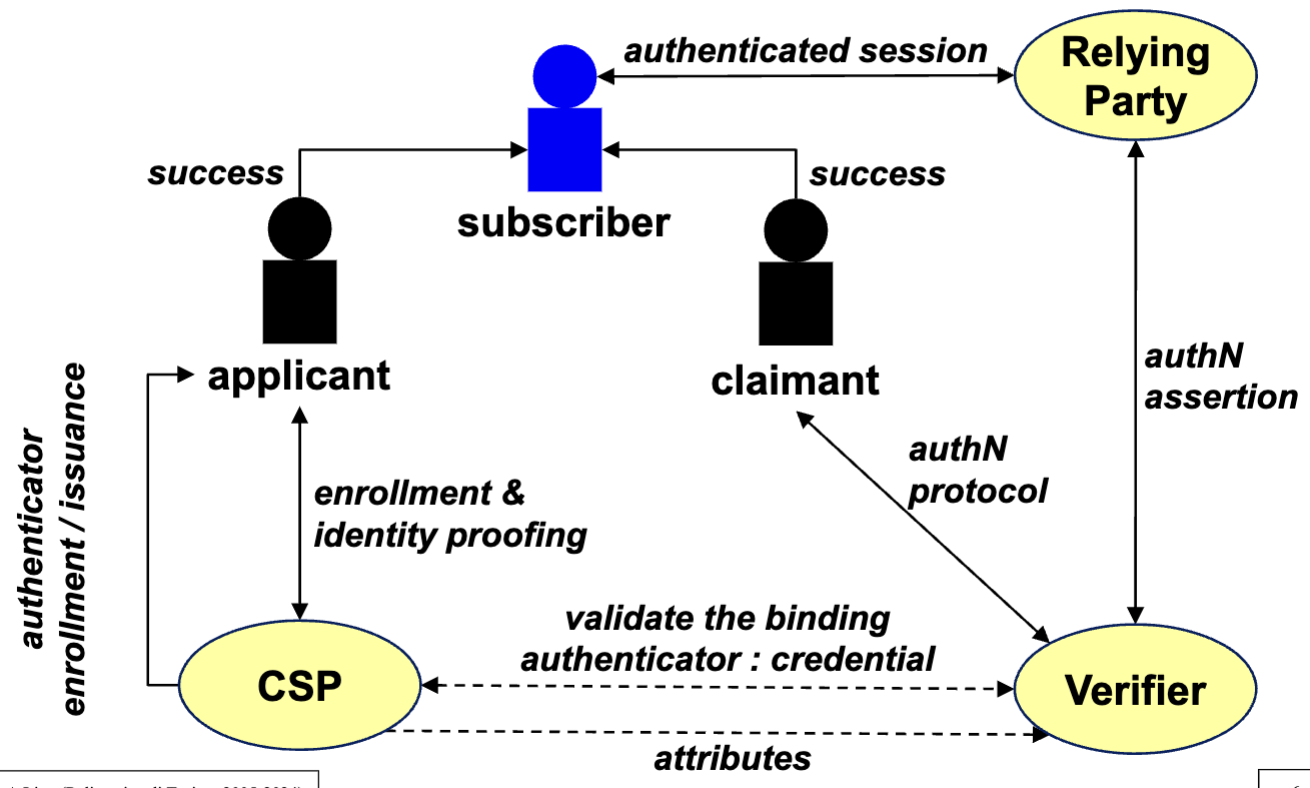
\includegraphics[width=0.6\linewidth]{Images/Authentication/auth_model.png}
    \caption{Digital Authentication Model}
\end{figure}

\begin{tcolorbox}[colback=blue!10!white, colframe=blue!50!white]
Credentials bind an authenticator to the subscriber's identity (e.g., the Public-key certificate binds the public key with specific attributes of the owner).
\end{tcolorbox}

\clearpage
\section{Generic Authentication Protocol}
\begin{enumerate}
    \item The verifier sends an authentication request to the user (claimant).
    \item The user sends his ID to the verifier.
    \item The verifier checks the ID against the stored credential data. Then, it sends a proof request (“Is this really you?”) to the user.
    \item The user sends an authentication response by submitting the appropriate authenticator $f(S_{UID})$(e.g., password, OTP, fingerprint) (Better if the channel is secure).
    \item The verifier checks the submitted response against the stored credential data (Mapped as UID:f($S_{UID}$)).
\end{enumerate}

\begin{figure}[H]
    \centering
    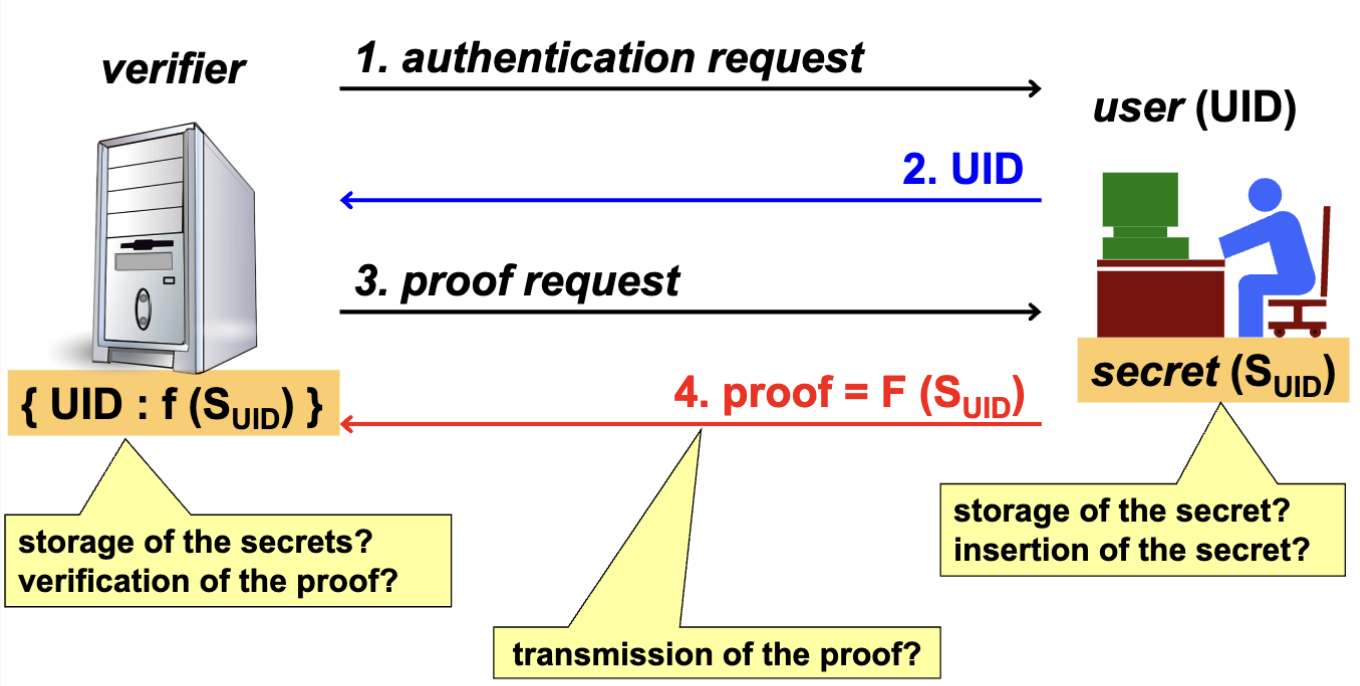
\includegraphics[width=0.5\linewidth]{Images/Authentication/authNprot.png}
    \caption{Generic Authentication Protocol}
\end{figure}

\subsection{Password-based Authentication}
The user's secret is the password. 
\begin{multicols}{2}
\raggedcolumns

    The verifier may have stored the password:
    \begin{itemize}
        \item In cleartext.
        \item One-way hashed.
    \end{itemize}
\columnbreak

\begin{figure}[H]
    \centering
    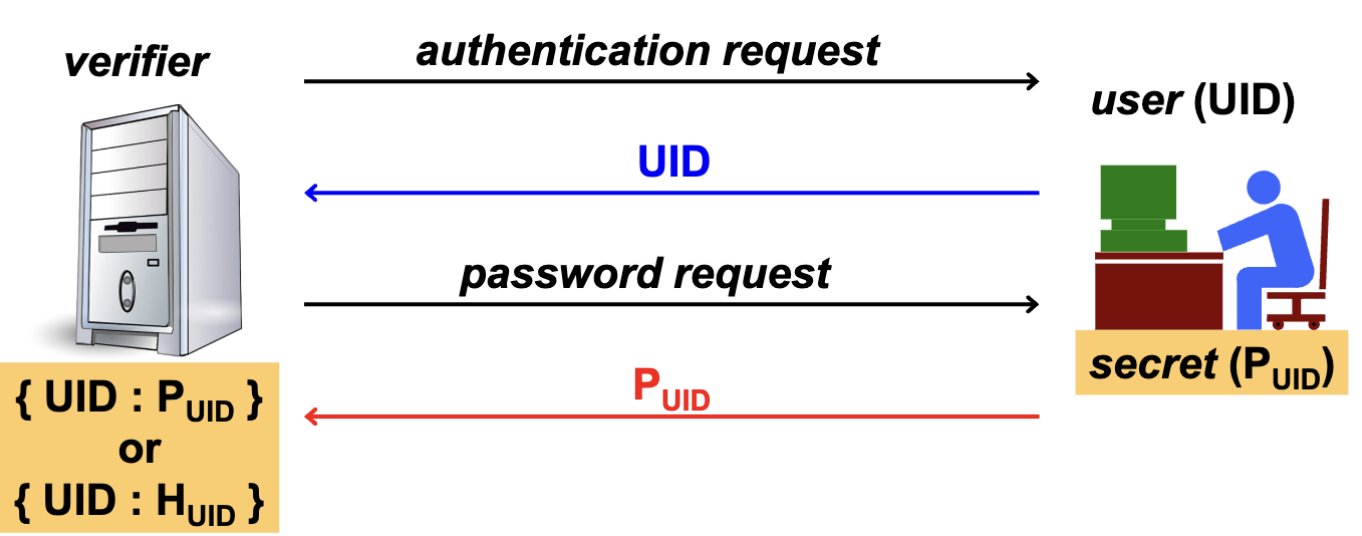
\includegraphics[width=\linewidth]{Images/Authentication/pb_authn.png}
    \caption{Password-based Authentication}
\end{figure}
\end{multicols}
In order to verify the proof given by the user, the verifier must either check if the password is the same as the one stored or hash the password and compare the digest with the stored hash.

\begin{tcolorbox}[colback=red!10!white, colframe=red!70!black, coltitle=white, title=Beware]
Even if the password is hashed, it is still vulnerable. For example, the attacker can use a dictionary attack or a brute-force attack.
\end{tcolorbox}




\clearpage
\begin{multicols}{2}
    \center{\subsubsection*{Reusable Passwords}}
    Reusing passwords can be dangerous:
    \begin{itemize}
        \item Password sniffing.
        \item Password DB attacks.
        \item Password guessing.
        \item Password enumeration (brute force attack): This occurs in the case of length-constrained passwords (or when fewer subsets of characters are available), or when the authentication protocol does not block multiple attempts.
        \item Password duplication: The same password is used for different services.
        \item Cryptography aging: In future years, cryptographic algorithms may become weak due also to the increasing computational power.
        \item Password capture (via spoofing or phishing).
        \item MITM attacks.
    \end{itemize}
    \columnbreak

    \center{\subsubsection*{Best Practices}}
    \begin{itemize}
        \item Alphabetic characters (upper and lower case) + digits + special characters.
        \item Must be at least 8 characters long (Brute force attack).
        \item Never use dictionary words.
        \item Frequently changed (but not too frequently).
        \[ \text{Password Age } \Delta t \le T_A =  {\text{items}^{\text{length}} \over 2}  \]
        \item Find alternative authentication methods (e.g., biometrics).
    \end{itemize}
    
\end{multicols}

\subsection*{Password Storage}
\begin{multicols}{2}
    Server-side password storage:
    \begin{itemize}
        \item NEVER in cleartext.
        \item Digest of the password (Dictionary attack, also with Rainbow Table).
        \item "Salted" hash: $H(Salt || Password)$.
    \end{itemize}
    
    \columnbreak

    Client-side password storage:
    \begin{itemize}
        \item Should be only in the user's hand ... but too many passwords.
        \item Use an encrypted file or a password wallet/manager.
    \end{itemize}
\end{multicols}

\begin{tcolorbox}[colback=blue!10!white, colframe=blue!50!white]
For Dictionary Attack and Rainbow Table, the attacker can use a precomputed table of hashes for all possible passwords. See Appendix A for more information.
\end{tcolorbox}

\subsection{Password Salting}
\begin{center}
    The only correct way to store passwords.\\ \textcolor{Blue}{Does not admit dictionary attacks or those based on rainbow tables(pre-computation attacks).}
\end{center}
How it works, for each user ID (UID) the Verifier:
\begin{itemize}
    \item Creates/asks the password.
    \item Generates a salt (different for each UID): A random (unpredictable) and long enough string, which should contain rarely used or control characters.
    \item Computes the Salted Hash of Password \(SHP = H(Salt || Password)\).
    \[\text{The salt is concatenated with the password.} \]
    \item Stores the tuple \((\text{UID, Salt, SHP})\).
\end{itemize}
Additional benefit: we have different SHP for users having the same password !

\vspace{0.3cm}

\begin{center}
    \textbf{Using the salted password in the authentication protocol:}
\end{center}
\begin{verbatim}
    Claimant > Verifier: (UID, pwd)

    Verifier:
        1. Checks if the UID is in the DB.
            1a. If not, abort: "AuthN Failure".
            1b. If yes, retrieves Salt from the DB.
        2. Computes SHP' = H(Salt || pwd).
        3. Compares SHP' with SHP.
            3a. If not equal, "AuthN Failure".
            3b. If equal, "AuthN Success".
\end{verbatim}

\begin{tcolorbox}[colback=red!10!white, colframe=red!70!black, coltitle=white, title=Beware]
Never give information about authentication failures. This could help attackers to guess the password.
\end{tcolorbox}

\subsection*{Passwords in Linux}
Originally stored in \texttt{/etc/passwd} (readable by everyone) hashed with a DES-based hash function named \texttt{crypt()}. Now stored in \texttt{/etc/shadow} (readable only by root).

\vspace{0.2cm}

Passwords are stored in the form:
\begin{itemize}
    \item \texttt{username:\$uid\$salt\$hashedpwd ...}
    \item Are used different hash functions depending on ID, for example:
    \begin{itemize}
        \item 1: MD5.
        \item 5: SHA-256.
        \item 6: SHA-512.
        \item y: YesCrypt.
    \end{itemize}
    \item If \texttt{\$uid\$salt} is absent then the old DES-based hash is used, with 12-bit salt, pwd truncated to 8 characters \textcolor{Red}{(not secure!!)}.
\end{itemize}

If you want to try yourself, you can use:
\begin{lstlisting}[style=bashStyle]
# gain root access
sudo su
# add user w/o pwd
sudo adduser test1 --disabled-password
# create pwd string with selected hash algo and salt
mkpasswd --method=md5 --salt=coolsalt 1234

# view the hash of 1234
echo -n 1234 | openssl dgst -md5
# in the /etc/shadow file you would see: 
#       $1$coolsalt$qTXiZzGn08J.xYkV1ce1y1:...
#   IDK the manual-hashed password don't correspond to the one given by mkpasswd ... correct me if I'm wrong
\end{lstlisting}

\subsection*{Passwords in MySQL}
Username and password are stored in the \texttt{mysql.user} table. MySQL (from v4.1) uses a double hash (\textcolor{Red}{not salted!!}) to store the password.
\[SHA1(SHA1(password)) \qquad \text{Very Poor Solution...}\]
\begin{lstlisting}[style=bashStyle]
# perform the double (but different) hash on the password
echo -n 'password' | openssl sha1 -binary | openssl sha1 -hex
# the stored output is: 2470c0c06dee42fd1618bb99005adca2ec9d1e19

\end{lstlisting}

\section{Strong (Peer) Authentication}
"Strong Authentication" is often requested in many specifications, but has never been defined in a standard way. It is often used to indicate that the authentication process is based on more than one factor.

\subsection*{ECB Definition}
\begin{center}
    (European Central Bank Definition)
\end{center}
Some elements of the ECB definition:
\begin{itemize}
    \item Strong customer authentication is a procedure based on the use of two or more of knowledge, ownership, and inherence. 
    \item The elements selected must be mutually independent (the breach of one does not compromise the others).
    \item At least one element should be non-reusable and non-replicable (except for inherence), and not capable of being surreptitiously stolen via the internet.
    \item The strong authentication procedure should be designed in such a way as to protect the confidentiality of the authentication data.
\end{itemize}

\subsection*{PCI-DSS Definition}
\begin{center}
    (Payment Card Industry Data Security Standard Definition)
\end{center}
PCI-DSS requires strong authentication for access to Cardholder Data Environment (CDE). It is defined for:
\begin{itemize}
    \item Remote access from trusted or untrusted networks.
    \item By users, third-parties (e.g. maintenance) and administrators.
    \item Exception: direct console access (physical security).
\end{itemize}
Compulsory after 2018.
\begin{tcolorbox}[colback=red!10!white, colframe=red!70!black, coltitle=white, title=Beware]
Multi-factor authentication is NOT twice the same factor (e.g., two passwords).
\end{tcolorbox}

\subsection*{Other Definitions}
Strong authentication as:

\vspace{0.3cm}

\blockquote[Handbook of Applied Cryptography]{A cryptographic challenge-response identification protocol.}

\vspace{0.3cm}

\noindent More in general:

\blockquote{Technique resisting to a well-defined set of attacks.}

\vspace{0.3cm}


In conclusion, an authentication (authN) technique can be regarded as strong or weak depending on the \textbf{attack model and the system properties}. For example, users of Internet banking services would probably prefer the ECB definition, while employees of PSP (Payment Service Providers) would prefer the PCI-DSS definition.

\section{Challenge-Response Authentication}
\begin{center}
    CRA - General Model
\end{center}

\begin{multicols}{2}
\begin{itemize}
    \item The claimant tries to enter a system with his User ID.
    \item The verifier sends a challenge (should be a nonce, to avoid replay attacks) to the claimant.
    \item The claimant replies with the solution computed using some secret knowledge and the challenge.
    \item The verifier compares the response with a solution computed  via a secret associated to the claimant.
\end{itemize}

\columnbreak

    \begin{figure}[H]
        \centering
        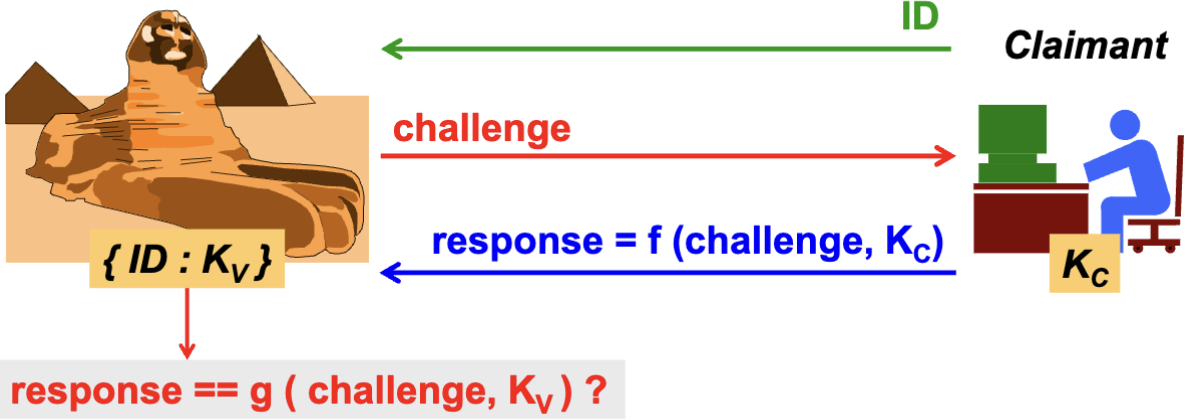
\includegraphics[width=\linewidth]{Images/Authentication/CRA.png}
        \caption{Challenge-Response Authentication model}
    \end{figure}
\end{multicols}

\subsection*{CRA - General Issues}
\begin{itemize}
    \item The challenge must be non-repeatable to avoid replay attacks. Usually the challenge is a (random) nonce (replay attacks).
    \item The function $f$ must be non-invertible (one-way function) otherwise, a listener can record the traffic and easily find the shared secret (sniffing attacks).
\end{itemize}

\subsection{Symmetric CRA}
Claimant and Verifier share a secret key \(K_{ID}\) (e.g., a password or a key).


\begin{multicols}{2}

    \begin{itemize}
        \item A challenge is sent to the claimant.
        \item The claimant computes the response as \(response = f(K_{ID}, challenge)\). Then sends it to the verifier.
        \item The verifier computes the expected response as \(response' = f(K_{ID}, challenge)\) and compares it with the received response.
    \end{itemize}
    
\columnbreak

    \begin{figure}[H]
        \centering
        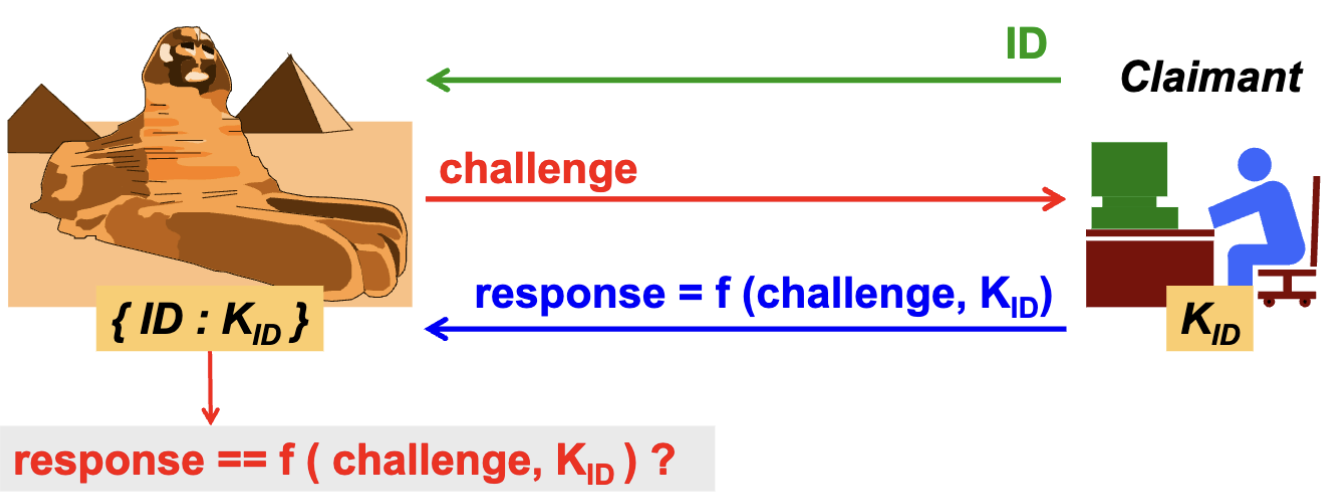
\includegraphics[width=\linewidth]{Images/Authentication/symCRA.png}
        \caption{Symmetric Challenge-Response Authentication}
    \end{figure}
\end{multicols}

\subsection*{Symmetric CRA - General Issues}
The easiest implementation uses a hash function (e.g. SHA1, deprecated). $K_{ID}$ must be known in cleartext to the verifier (possible attacks). SCRAM (Salted Challenge Response Authentication Mechanism) is a better solution, by using hashed passwords at the Verifier side (offers also secure channel binding and mutual authentication).

\clearpage
\subsection{Mutual Symmetric Challenge-Response Authentication} 
\begin{center}
    General exchange - Deprecated.\\
    Both parties authenticate each other using a shared \\secret key and challenge-response mechanisms.\\ 
\end{center}
\begin{tcolorbox}[colback=red!10!white, colframe=red!70!black, coltitle=white, title=Beware]
The protocol (and so its related problem) relies on demonstrating the knowledge of the shared secret.
\end{tcolorbox}

\begin{multicols}{2}

    \begin{center}
        {\large{\textbf{v1:}}}
    \end{center}
    \begin{itemize}
        \item Only the initiator (of the communication) provides explicitly its (claimed) identity.
    \end{itemize}
    \begin{figure}[H]
        \centering
        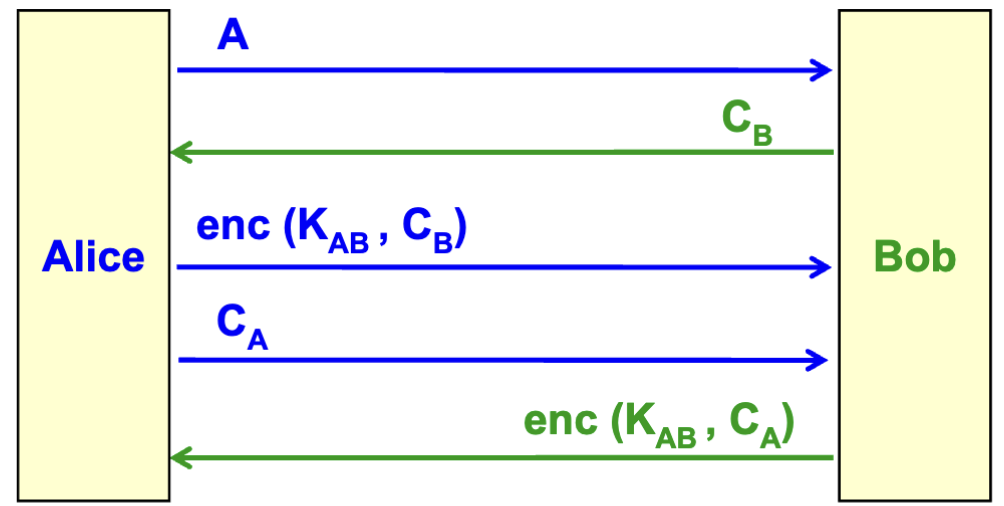
\includegraphics[width=\linewidth]{Images/Authentication/msCRA.png}
        \caption{Mutual Symmetric Challenge-Response Authentication first version}
    \end{figure}
    \columnbreak

    \begin{center}
        \large{\textbf{v2:}}
    \end{center}
    \begin{itemize}
        \item Only the initiator (of the communication) provides explicitly its (claimed) identity.
        \item Fewer messages.
        \item Better performance, but still no impact on security.
    \end{itemize}

    \begin{figure}[H]
        \centering
        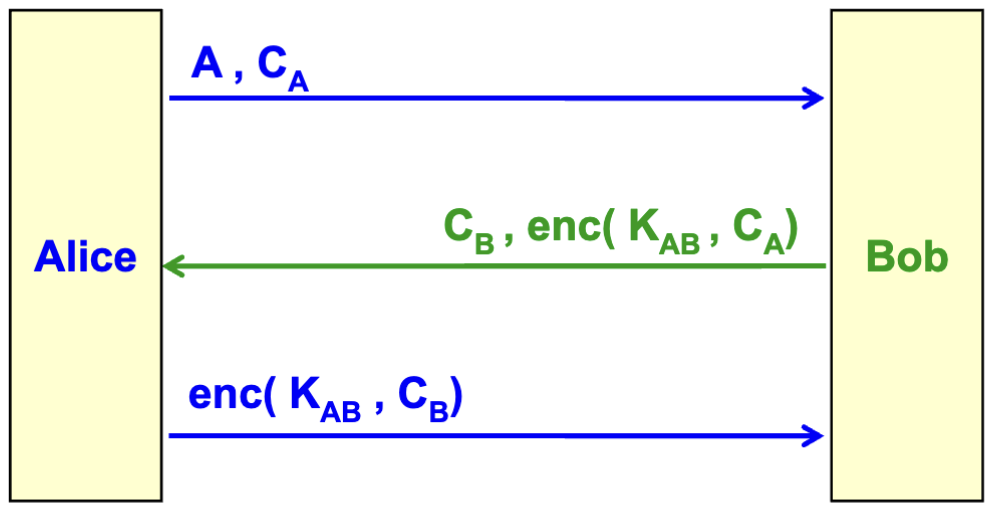
\includegraphics[width=\linewidth]{Images/Authentication/msCRAv2.png}
        \caption{Mutual Symmetric Challenge-Response Authentication second version}
    \end{figure}
    
\end{multicols}

\subsubsection*{Mutual Symmetric CRA - Process}
\begin{center}
    v1:
\end{center}
Alice to Bob authentication:
\begin{itemize}
    \item The initiator (Alice) sends her ID to the responder (Bob).
    \item Bob sends a challenge to Alice.
    \item Alice encrypts the challenge with her secret key and sends it to Bob.
    \item Bob decrypts the response and checks if it is correct.
\end{itemize}
\dots\ Bob to Alice authentication:
\begin{itemize}
    \item Alice sends a challenge to Bob.
    \item Bob encrypts the challenge with his secret key and sends it to Alice.
    \item Alice decrypts the response and checks if it is correct.
\end{itemize}

\subsection*{Mutual Symmetric CRA - Attack}
\begin{center}
    Exploits the fact that the same key is used for both directions.
\end{center}




\begin{multicols}{2}

    \begin{itemize}
        \item Mike (the attacker pretending to be Alice) creates a first connection by sending Alice's identifier $A$ along with a random challenge $C_A$ to Bob.
        \item Bob replies with the encrypted challenge-response and a new challenge $C_B$ (due to mutual authentication).
        \item Mike stores the new challenge, then\dots
    \end{itemize}
    \columnbreak

    \begin{figure}[H]
        \centering
        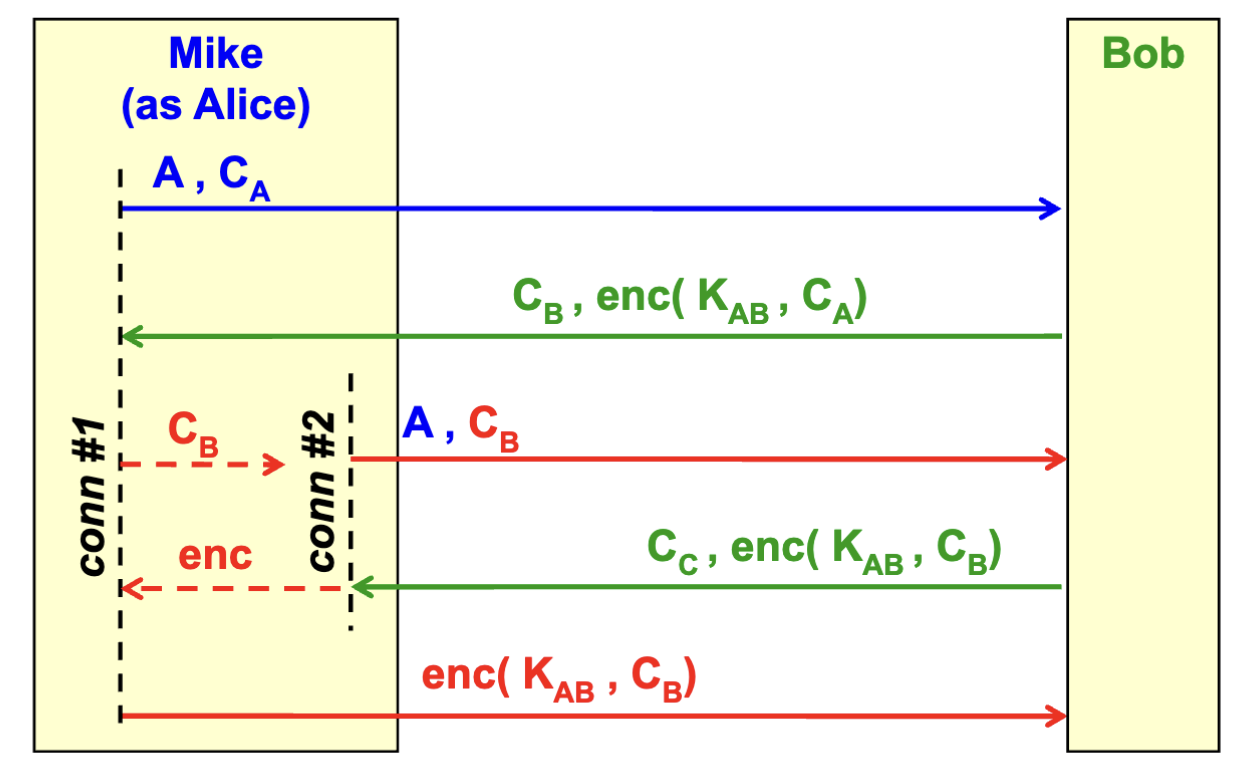
\includegraphics[width=\linewidth]{Images/Authentication/msCRAatt.png}
        \caption{Attack to Mutual Symmetric CRA}
    \end{figure}
\end{multicols}
\begin{itemize}
    \item Mike creates a second connection by sending Alice's identifier $A$ and replaying ($\ne$ replying) the challenge $C_B$, which was received earlier from Bob.
    \item Bob replies with the encrypted challenge $C_B$(the previous one sent by Bob) and a new challenge $C_C$.
    \item Mike reuses the first connection to send the encrypted challenge-response to Bob, ensuring the mutual authentication.
\end{itemize}

\subsubsection{Global System for Mobile Communications (in)Security}
\begin{center}
    GSM insecurity.
\end{center}
GSM uses three secret algorithms:
\begin{itemize}
    \item $A8$ for symmetric key generation (in the SIM).
    \item $A3$ for authentication (in the SIM).
    \item $A5$ (stream cipher) for encryption (in the mobile device).
\end{itemize}
This is security-through-obscurity\footnote{The algorithms are secret, rather than depending on robust secrutiy measures.}\dots always a bad idea !
The three algorithms above are left to the choice of the MNO (Mobile Network Operator) and are not standardized.
\begin{tcolorbox}[colback=blue!10!white, colframe=blue!50!white]
$A8$ and $A3$ are usually built upon the COMP128 (secret) function.
\end{tcolorbox}

\clearpage
\subsubsection*{GSM Authentication Mechanism}
\begin{multicols}{2}

    The authentication protocol uses a symmetric challenge-response mechanism to authenticate the Mobile Station (MS) via its SIM card to the Base Station (BS). The process works as follows:
\columnbreak

    \begin{figure}[H]
        \centering
        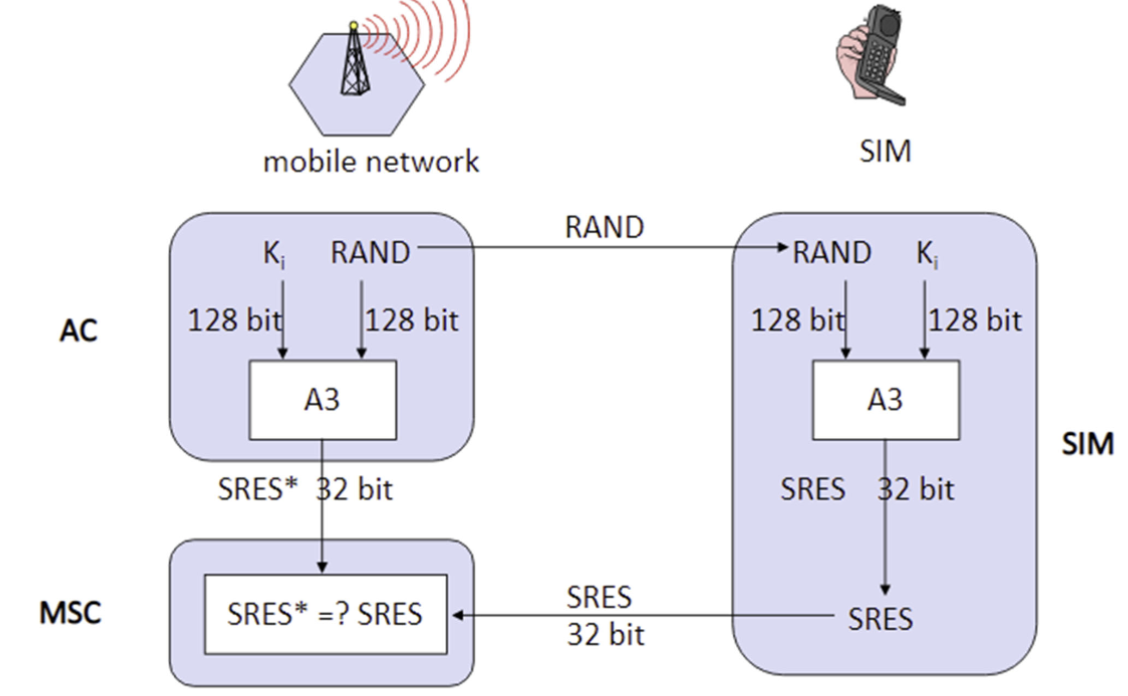
\includegraphics[width=\linewidth]{Images/Authentication/gsm_authn.png}
        \caption{GSM Authentication Mechanism}
    \end{figure}
\end{multicols}

\begin{itemize}
    \item The BS sends to the SIM card a random challenge $C$ of 128 bits. 
    
    \hspace*{1cm} This challenge is intended to verify the possession of \\ \hspace*{3cm} the shared secret key  $K_i$  stored securely on the SIM.
    \item The SIM computes the response as $SRES = A3(K_{i}, C)$ of 32 bits.
    \begin{itemize}
        \item COMP128-1 is weak \dots with chosen-challenge (and differential cryptanalysis) $150k$ challenges are enough to compute the secret key $K_i$.
        \item \dots\ then an attacker could clone the SIM card and \\\hspace*{4cm} decrypt the traffic by computing $K_c$.
        
        $K_c$  is a session key established between the Mobile Station (MS) and the Base Station (BS), and it is derived from the secret key  $K_i$  (stored on the SIM card) and the random challenge $C$  sent by the BS.
    \end{itemize}
\end{itemize}

\subsection{Asymmetric CRA}
\begin{center}
    Authentication based on public-key cryptography.

    Remember that the PK certificate must be valid (not revoked) and trusted.
\end{center}

\begin{multicols}{2}

    \begin{itemize}
        \item The Claimant sends his public-key certificate to the Verifier.
        
        The certificate contains the public key $ID.PK$ and the claimant's ID.
        \item The verifier encrypts a random nonce $R$ with the claimant's public key $ID.PK$ (asymm. encryption) and sends it to the claimant.
        \item The claimant decrypts the nonce with his private key $ID.SK$ and sends it back to the verifier.
    \end{itemize}

    \columnbreak
\begin{figure}[H]
    \centering
    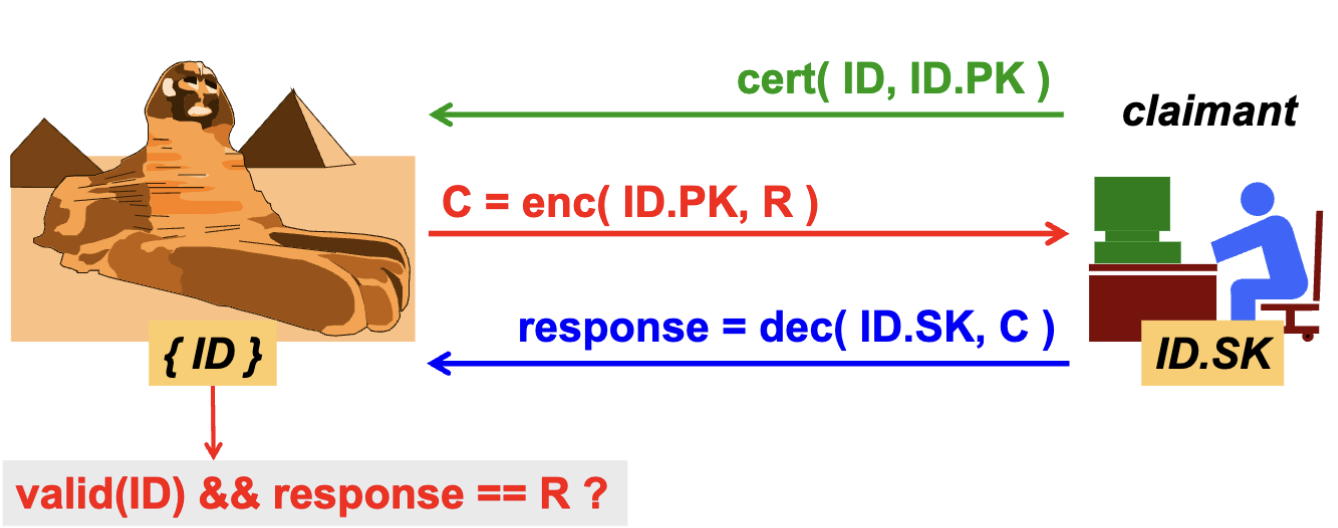
\includegraphics[width=\linewidth]{Images/Authentication/asymmCRA.png}
    \caption{Asymmetric Challenge-Response Authentication}
\end{figure}

\end{multicols}

At the end, the Verifier checks if the received nonce is the same as the one sent. The claimant has demonstrated the possession of the private key associated with the public key in the certificate.

\subsection*{Asymmetric CRA - Analysis}
\begin{itemize}
    \item The strongest mechanism.
    \item Does not require secret storage at the Verifier side.
    \item Applications: Implemented for peer authentication (client and server) in IPsec, SSH, TLS.
    \item Cornerstone for user authentication in FIDO (Fast Identity Online).
\end{itemize}
\subsection*{Asymmetric CRA - General Issues}
\begin{itemize}
    \item Slow.
    \item If designed inaccurately may lead to an involuntary disclosure of the private key.
    \item PKI (Public Key Infrastructure) issues (trusted root, name constraint, revocation, etc.).
    
    This could be avoidable if the Verifier stores $ID.PK$ in a secure way \dots \ but this moves equivalent PKI effort to the Verifier.
\end{itemize}

\section{One-Time Password}
\begin{center}
    OTP - General Model
\end{center}
\begin{multicols}{2}

    \begin{itemize}
        \item The verifier sends an authentication request to the user.
        \item The user sends his ID to the verifier.
        \item The verifier requests a one-time password (OTP) to the user (no.48 in the figure's case).
        \item The server computes the expected value of P48 in real-time using the shared secret $S_{UID}$, the counter, and a function $p$.
        
        \begin{itemize}
            \item The function $p$ is a \textbf{MAC} function (e.g., HMAC-SHA1). Which provides authentication and integrity for the data. Possible implementation: keyed-digest (e.g. HMAC).
        \end{itemize} 
    \end{itemize}

    \columnbreak

    \begin{figure}[H]
        \centering
        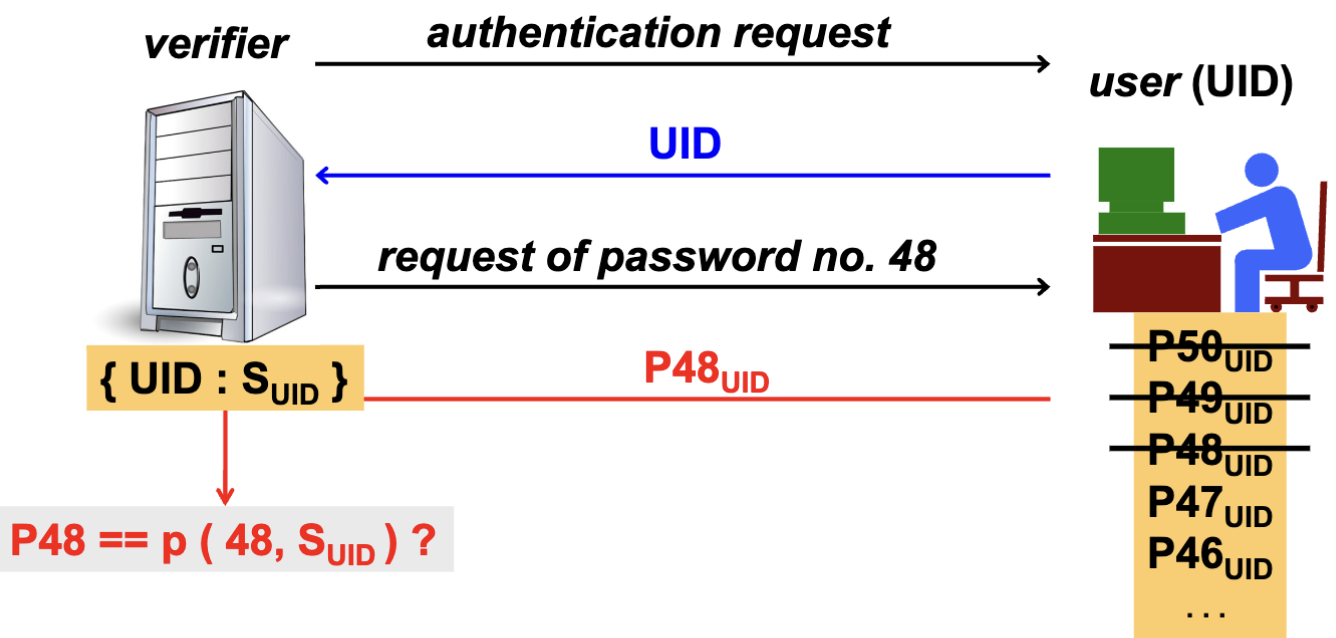
\includegraphics[width=\linewidth]{Images/Authentication/OTP.png}
        \caption{One-Time Password}
    \end{figure}
    
\end{multicols}
If the provided password  $P48_{UID}$  matches the server's computed value  $p(48, S_{\text{UID}})$, the user is authenticated successfully.

\clearpage
\subsection*{OTP - Analysis}
\begin{itemize}
    \item The password is valid only for one run of the authentication protocol (Next run requires a new password).
    \item Immune to sniffing.
    \item Subject to MITM (needs Verifier to be authenticated).
    \item Difficult provisioning to the subscribers/users: Lots of passwords to remember, password exhaustion (time limit for use).
    \item Difficult password insertion: Verbose and mixed (Contains random characters to avoid guessing attacks) on purpose.
\end{itemize}

\subsection*{OTP - Provisioning to Users}
On naive systems, or insecure/untrusted workstation:
\begin{itemize}
    \item Paper sheet of precomputed passwords ("password cards").
    \item Hardware authenticators ("crypto tokens")(e.g., RSA SecurID or Google authenticator).
\end{itemize}
On intelligent and secure/trusted workstation:
\begin{itemize}
    \item Automatically computed by an ad-hoc application.
    \item Typically, the OTP is generated by a smartphone app.
\end{itemize}

\subsection{The Secure Key System}
\begin{center}
    S/KEY System for Off-line/Precomputed One-Time Passwords.
\end{center}

First OTP definition and implementation by Bell Labs (1981). 
\begin{itemize}
    \item The user generates a secret $S_{ID}$ and a sequence of $n$ OTPs.
    \[
        \begin{aligned}
            &P_1 = h(S_{ID}) \\
            &P_2 = h(P_1) \\
            &\dots \\
            &P_n = h(P_{n-1})\\\\
            \text{h is a } &\text{hash } \text{function (e.g. md4).}
        \end{aligned}
    \]
    \item The Verifier stores the last one OTP used $P_n$: This password will never be used directly for authentication.
    \item Verifier requests $P_{n-1}$, and receives $X$ (reverse order of requests).
    \[
        P_n \ne h(X)\quad ?\quad \text{"OK, store X as } P_{n-1}\text{"} : \text{"AuthN Failure"}
    \]
    In this way the Verifier has no need to know the user's secret and only the user knows all passwords.
\end{itemize}

\begin{figure}[H]
    \centering
    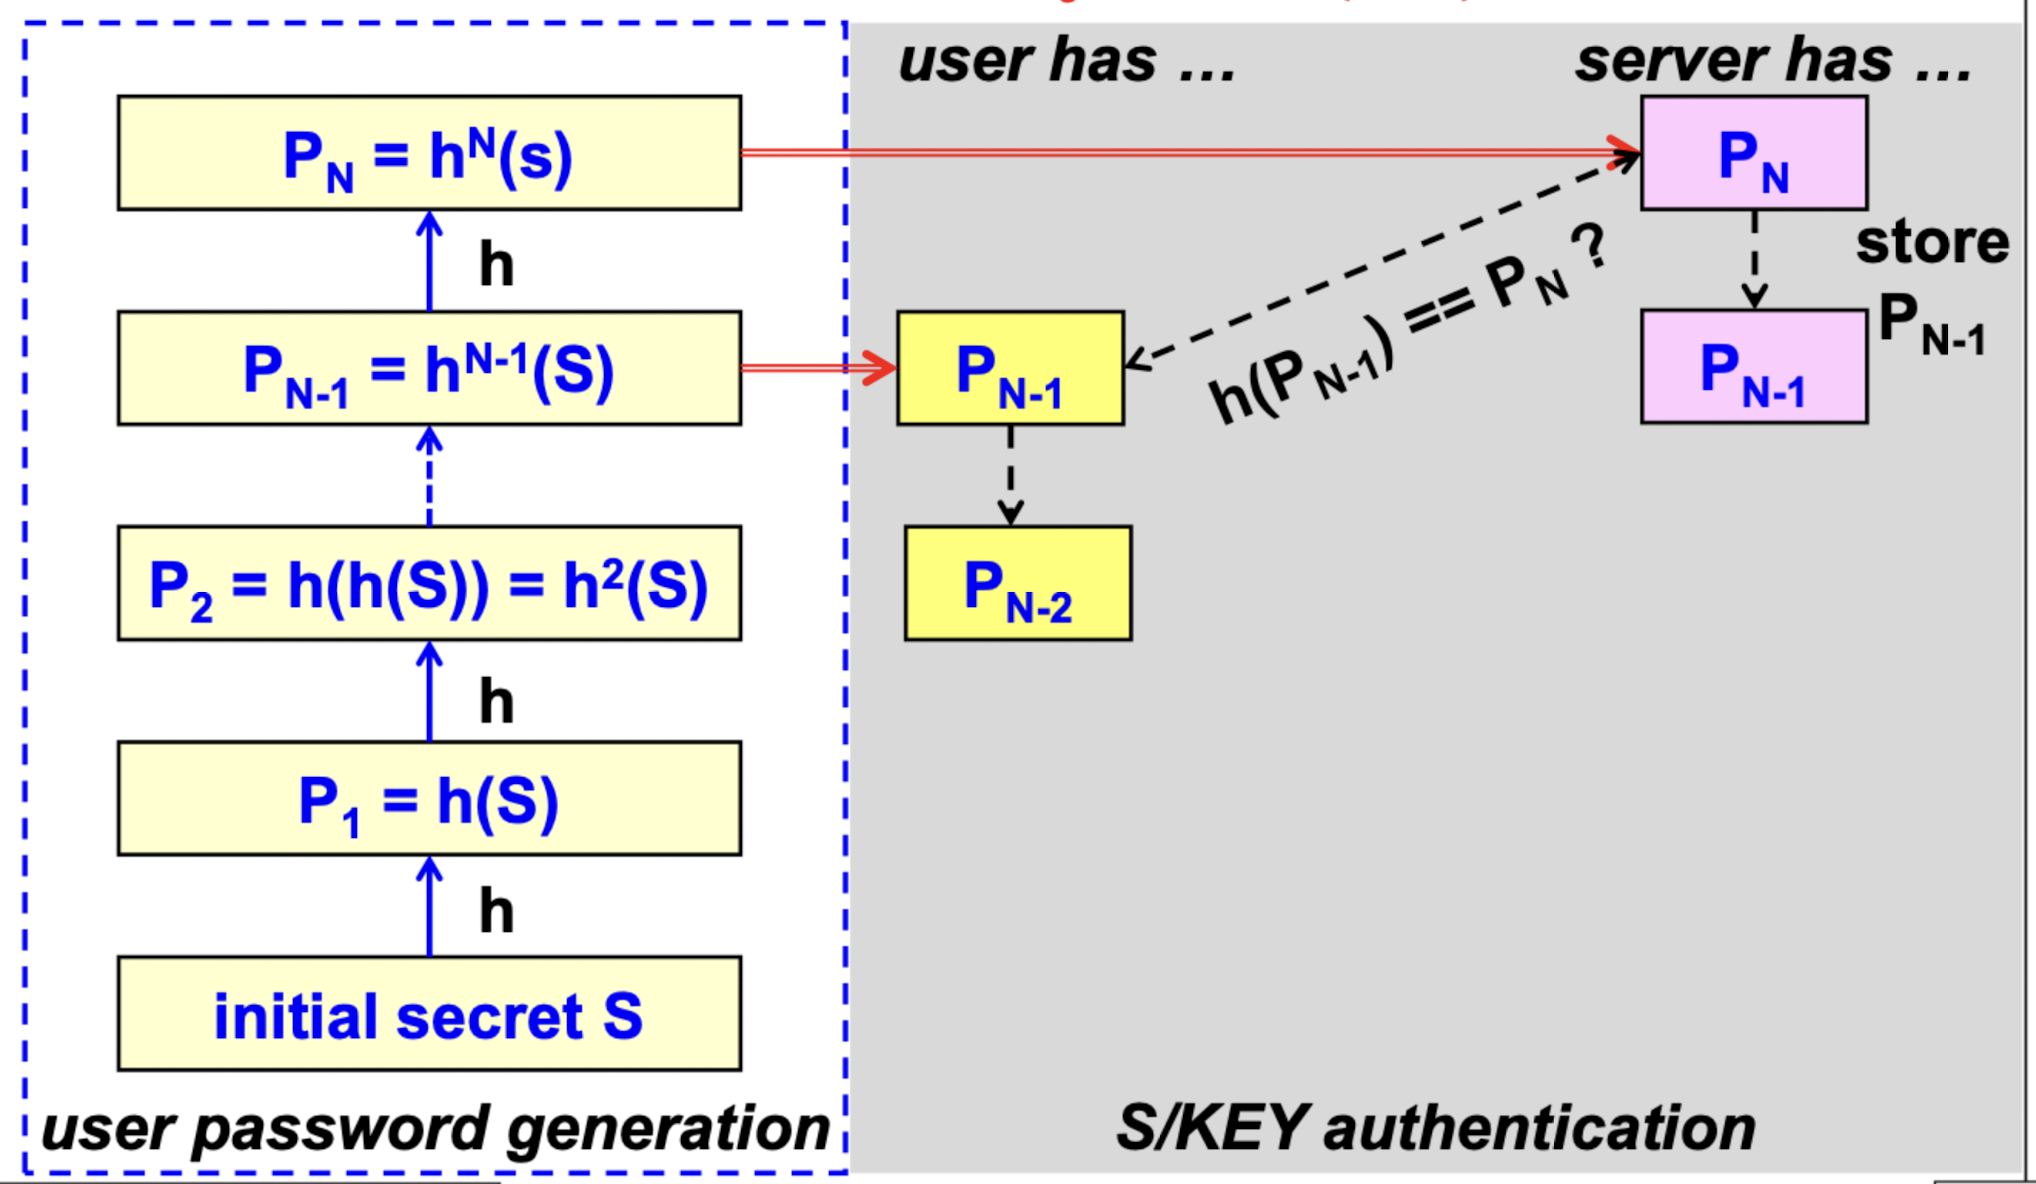
\includegraphics[width=0.5\linewidth]{Images/Authentication/skey.png}
    \caption{Secure Key System Model}
\end{figure}

\subsubsection*{S/KEY - Password-Chain Generation}
\begin{center}
    The real implementation uses a seed and a pass phrase.
\end{center}
\begin{enumerate}
    \item The user generates a Pass Phrase (PP) $S_{ID}$: Minimum 8 characters long, mixed, and secret! (if exposed the security of S/KEY is compromised).
    \item PP is concatenated with a server-provided seed 
    
    The seed is not secret; it is sent in cleartext from the server to the client. It allows the reuse of a passphrase (PP) (using different seeds).
    \item A 64-bit quantity is extracted from the $md4(PP||seed)$ hash (output of 128-bit).
    
    This is achieved by XORing the first 32-bit group with the third 32-bit group, and the second 32-bit group with the fourth 32-bit group.
\end{enumerate}

\subsubsection*{S/KEY - Passwords}
\begin{itemize}
    \item 64-bit passwords are a compromise:\\\hspace*{3cm}Neither too long (complex) nor too short (easy to guess).
    \item Entered as a sequence of 6 short English words\footnote{Instead of just random bits, to make them easier for users to remember.} chosen from a dictionary of 2048 \\(e.g. 0="A", 1="ABE", 2="ACE", 3="ACT", 4="AD", 5="ADA")
    
    \dots Client and Server must share the same dictionary.
    \\\hspace*{1cm} e.g. text-password: "YOU SING A NICE OLD SONG"
    \\\hspace*{1cm} e.g. numeric-password (hex): "1D6E5001884BD711"
\end{itemize}
\subsection{Time-Based One-Time Password}
\begin{center}
    TOTP - General Model.
\end{center}
The OTPs depend upon time (e.g. valid for 30 seconds) and the claimant's secret.
\[
    \boxed{OTP =h(S_{ID}, t)}
\]
$h$ : A cryptographic hash or HMAC (better) function used to generate the token.\\
$t$: The current time (e.g., in seconds or milliseconds).
\begin{multicols}{2}

    \begin{itemize}
        \item The Verifier sends an authentication request to the user.
        \item The Claimant sends his $ID$ and $X$ to the Verifier. 
        \item The Verifier also computes $X$, but using the stored information, and compares it with the received one.
    \end{itemize}
\columnbreak

    \begin{figure}[H]
        \centering
        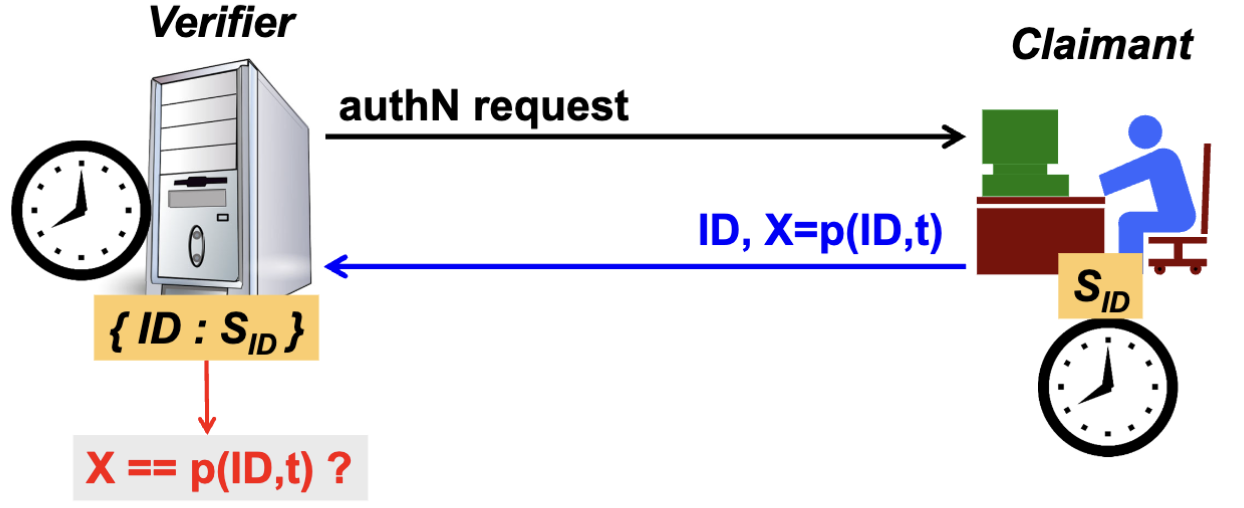
\includegraphics[width=\linewidth]{Images/Authentication/totp.png}
        \caption{Time-Based One-Time Password}
    \end{figure}
\end{multicols}

\subsection*{Time-Based OTP - Analysis}
\begin{itemize}
    \item Requires clock synchronization or keeping track of time-shift for each subscriber.
    
    Desynchronization can be a cause to DDoS attacks or passwords stealing.
    \item Requires time-slot and authentication window management.
    
    Tolerance window for time-based authentication:
    \\\hspace*{1cm}(It ensures flexibility when verifying the validity of a time-based proof or token  X)
    \[
        X==p(\text{ID}, t) \quad \| \quad X == p(\text{ID}, t-1) \quad \| \quad X == p(\text{ID}, t+1)
    \]
    \item Only one OTP per time-slot (typically 30 seconds or 60s).
    \item Time attacks against subscribers and Verifier: For example, fake NTP (Network Time Protocol) server.
    \item Sensitive database at the Verifier side  (e.g. attack against RSA SecurID).
\end{itemize}
\begin{tcolorbox}[colback=blue!10!white, colframe=blue!50!white]
Antennas can be used to synchronize the clocks of the devices.
\end{tcolorbox}

\subsubsection*{Time-Based OTP - RSA SecurID}
\begin{center}
    A concrete implementation of TOTP (Time-Based OTP).
\end{center}
\begin{itemize}
    \item The Claimant sends to the Verifier in clear: username, PIN, token-code (seed + current time). The token-code can comprehend the PIN also (if an authenticator with pinpad is used).
    \item Based on user and PIN the Verifier checks the token-code sent by the claimant against three possible time windows to account for clock drift:
    \begin{itemize}
        \item  $TC_{-1}$ : Token-code from the previous time window.
        \item $TC_0$ : Token-code from the current time window.
        \item $TC_{+1}$ : Token-code from the next time window.
    \end{itemize}
    \item "Duress Code": A special code that can be used to authenticate the user in case of coercion (apparently does the same as the normal code, but it triggers an alarm).
\end{itemize}
\subsubsection*{RSA SecurID - Architecture}

The RSA SecurID system is composed of:
\begin{itemize}
    \item Claimant: The user who wants to authenticate.
    \item ACE Client: Installed on the Relying Party. Establishes the connection with the claimant and forwards authentication information to the ACE server for verification.
    \item ACE Server: The core authentication verifier. Checks the validity of the SecurID token code, user credentials (PIN, etc.).
\end{itemize}
Left side of the figure \ref{fig:secarch} is a successful authentication, right side is a failed authentication.

\begin{figure}[H]
    \centering
    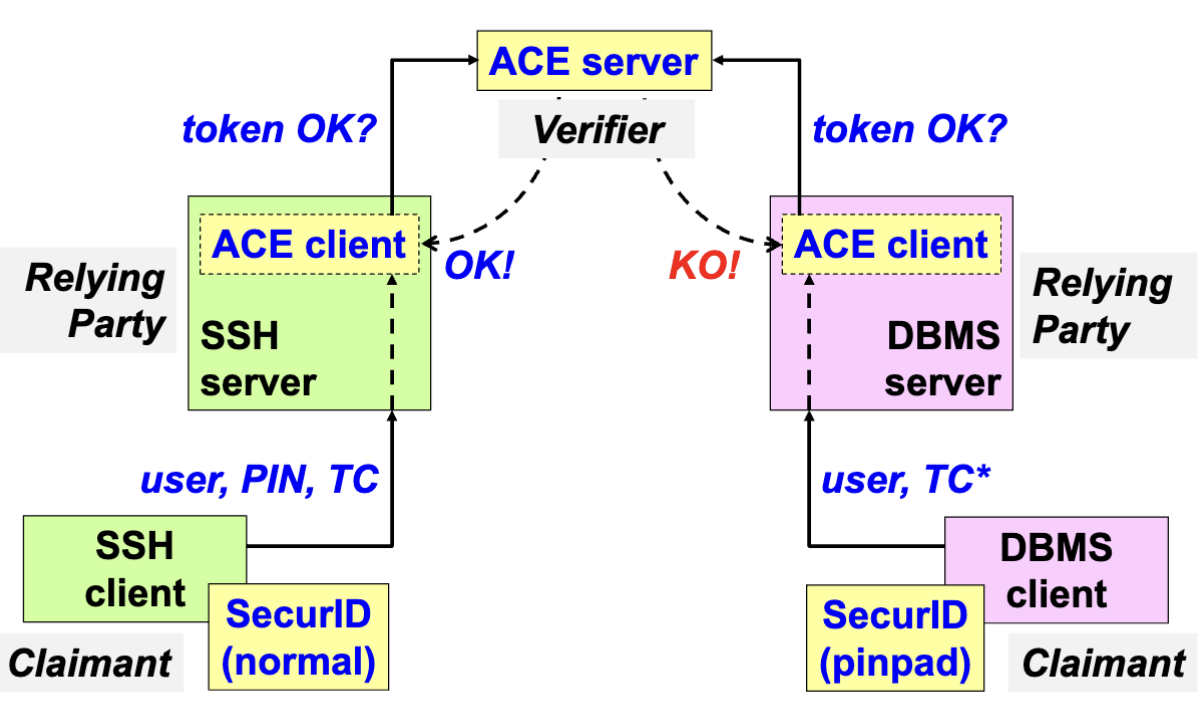
\includegraphics[width=0.5\linewidth]{Images/Authentication/secarch.png}
    \caption{RSA SecurID Architecture}
    \label{fig:secarch}
\end{figure}

\subsection{Event-Based One-Time Password}
\begin{center}
    Event-Based OTP - General Model.
\end{center}
The OTPs depend upon events (e.g. a button press) and the user's secret.
\begin{itemize}
    \item Uses monotonic integer counter $C$ as input besides the seed.
    \[
        \boxed{OTP = =h(S_{ID}, C)} \quad \text{with } C \in \mathbb{Z} \land\text { monotonic}
    \]
    \item Requires local computetion at the subscriber/claimant side.
    \item Because the counter is event-driven, the user can generate OTPs frequently without waiting for time slots (unlike time-based OTPs).
    \item OTPs can be generated in advance because they depend only on the counter value:
    \begin{itemize}
        \item Useful for travel: Users can carry pre-computed OTPs to avoid losing access (e.g., when they don't have their token).
        \item Security Risk: An adversary with temporary access to the authenticator can pre-compute OTPs, increasing the risk of misuse.
    \end{itemize}
    \item The counter on the user's device (subscriber) may become out of sync with the verifier (e.g. manual increments) so, the verifier must accommodate desynchronization by checking a range of counter values:
    \[
X == p(\text{ID}, C) \, \| \, X == p(\text{ID}, C+1) \, \| \, X == p(\text{ID},C+2) \, \| \, \dots
    \]
    How big should be the tolerance window? It depends on the application and the risk of desynchronization.
\end{itemize}

\subsection{Out-of-Band One-Time Password}
\begin{center}
    Out-of-Band OTP - General Model.
\end{center}

\begin{multicols}{2}

    \begin{itemize}
        \item What differs from the previous OTPs is the channel used to send the OTP, which must be secure and reliable.
        \item The verifier generates the OTP and sends it to the claimant via a different channel (e.g., SMS, email, or voice call): Risky due to problems of VoIP, mobile user identification, and SS7 (Signaling System 7) vulnerabilities.
        \item NIST SP800-63B states: PSTN (SMS or voice) as OOB channel is deprecated. Suggests using Push mechanism over TLS channel to registered subscriber devices.
    \end{itemize}
\columnbreak

    \begin{figure}[H]
        \centering
        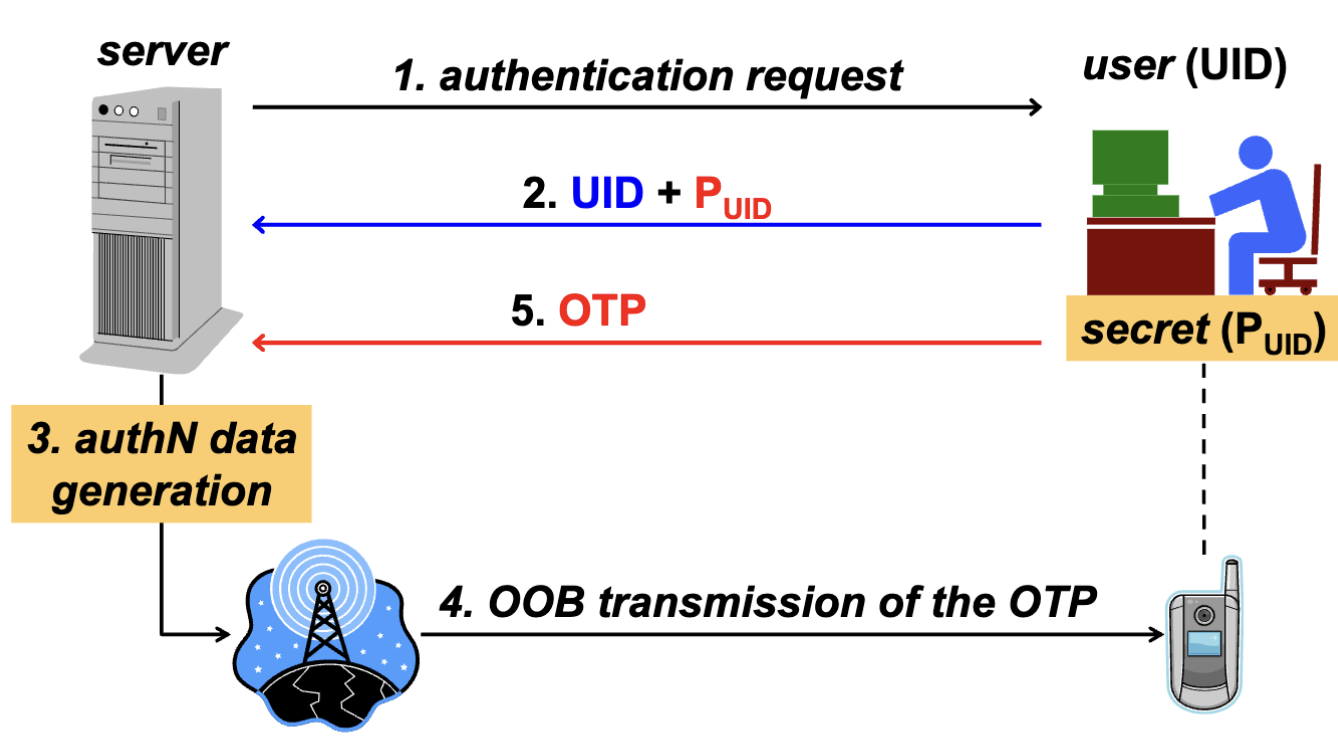
\includegraphics[width=\linewidth]{Images/Authentication/OOBotp.png}
        \caption{Out-of-Band One-Time Password}
    \end{figure}
\end{multicols}
\( \text{Assumptions: smart devices and network connectivity.} \)

\section{Two-/Multi-Factors Authentication}
\begin{center}
    2FA/MFA
\end{center}

\begin{itemize}
    \item Use more than one factor to authenticate the user: increased authentication strength and authenticator protection.
    \item PIN for authenticator protection:
    \begin{itemize}
        \item Transmitted along with OTP (secure channel).
        \item Used to compute the OTP itself.
        \item Used to unlock the authenticator (e.g., smart card), which can be very risky if:
        \begin{itemize}
            \item The lock mechanism is weak.
            \item There is no protection against multiple unlock attempts.
            \item Unlocking remains valid for a time window.
        \end{itemize}
    \end{itemize}
\end{itemize}
\section{Authentication of Human Beings}
How to authenticate a human being? The most common methods are:
\begin{itemize}
    \item CAPTCHA (Completely Automated Public Turing test to tell Computers and Humans Apart): A challenge-response test used to determine whether the user is human.
    \item Biometric techniques (e.g. fingerprint)
\end{itemize}

\subsection{Biometric Systems}
\begin{center}
    Identification, not only authentication.

    \textcolor{Red}{NOT REPLACEABLE}, to be used locally.
\end{center}
Consists of a measure of a user's biological characteristic. The most common biometric techniques are: 
\begin{itemize}
    \item Fingerprint recognition.
    \item Facial recognition.
    \item Iris scanning.
    \item Voice recognition.
    \item Hand geometry.
    \item Retinal scanning.
\end{itemize}
Each technique can potentially be circumvented by an attacker. For example, fingerprint recognition can be bypassed by using a fake fingerprint. The security of a biometric system depends on the uniqueness of the biometric characteristic and the robustness of the system. Additionally, the biometric authentication is \textcolor{Red}{NOT REPLACEABLE}.

\subsection*{Biometric Systems - Issues}
Parameters related to the accuracy of biometric systems:
\begin{multicols}{2}
    \raggedcolumns

    \begin{itemize}
        \item FAR (False Acceptance Rate): The probability that the system incorrectly accepts an unauthorized user ("False Positive").
        \item FRR (False Rejection Rate): The probability that the system incorrectly rejects an authorized user("False Negative").
    \end{itemize}
\columnbreak

    \begin{figure}[H]
        \centering
        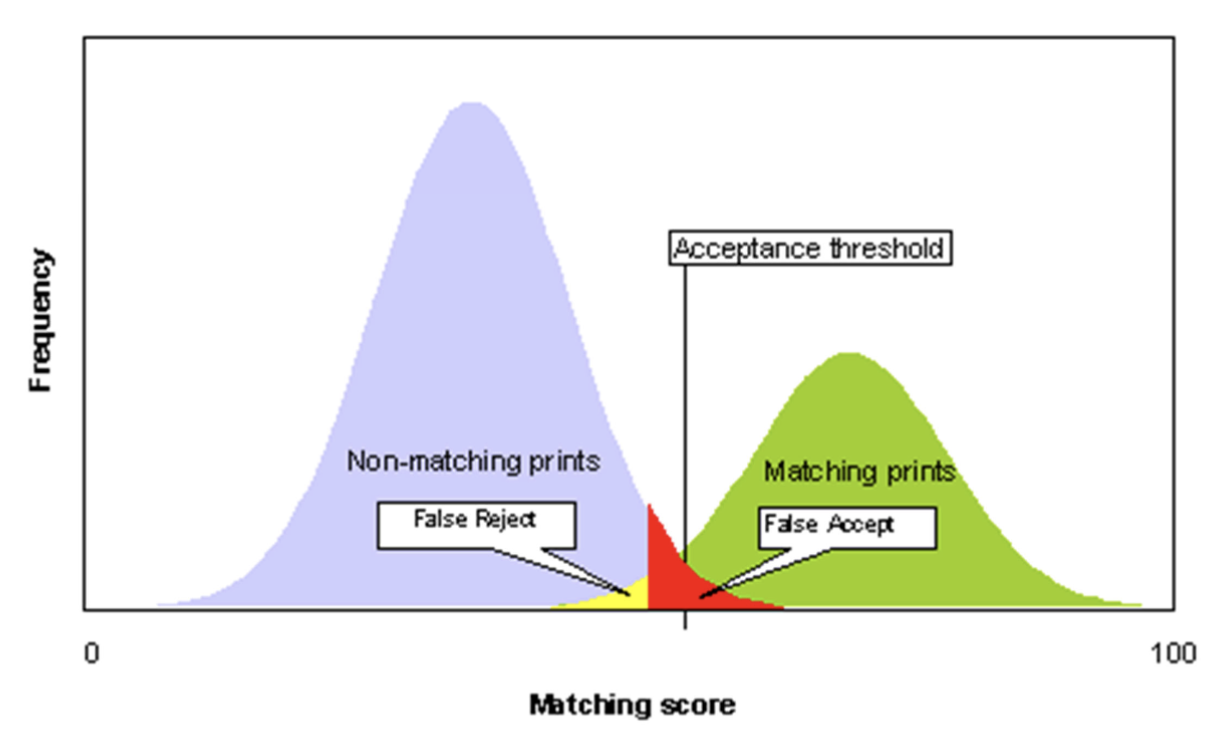
\includegraphics[width=\linewidth]{Images/Authentication/farrfrr.png}
        \caption{FAR and FRR}
    \end{figure}
\end{multicols}
FAR and FRR may be partly tuned, but they heavily depend on the cost of the system. Some variable biological characteristics are: finger wound, voice altered due to emotion or retinal blood pattern altered due to alcohol or drug.

\subsubsection*{Biometric Systems - Issues Analysis}

\begin{itemize}
    \item Psychological acceptance: Users may feel uncomfortable with biometric systems due to concerns about personal data collection, often referred to as the “Big Brother” syndrome. 
    \item Privacy: It's an identification (not just Authentication!!).
    \item Cannot be changed if copied, hence only useful to "locally" replace a PIN or a password.
    \item Lack of a standard API/SPI: high development costs and hevay dependence on single/few vendors.
\end{itemize}

\section{Kerberos}
\begin{center}
    Authentication System based on symmetric cryptography.
\end{center}



\begin{multicols}{2}
    \raggedcolumns

    \begin{center}
        Some key features:
    \end{center}
    \begin{itemize}
        \item Useful for non-HTTP services.
        \item The TTP (Trusted Third Party) substitutes the Verifier.
        \item \textbf{Client (peer) authentication is compulsory} (however, server authN is optional).
        \item The original version does not require Asymmetric Cryptography.
    \end{itemize}
\columnbreak

\begin{center}
    Definitions:
\end{center}
\begin{itemize}
    \item Realm (Kerberos Domain): A set of users and services that share the same Kerberos database.
    \item Credential: A set of information that proves the identity of a user.
    \[
        \text{user.instance@REALM}
    \]
    \item Ticket: A data structure used to authenticate a client to a server. It is encrypted with the symmetric key of the target server and is bound to the client's IP address.

\end{itemize}
\end{multicols}

\subsection*{Kerberos - Components}




\begin{multicols}{3}
    \raggedcolumns

\textbf{Authentication Server}
\hspace*{2.5cm}(AS)
\begin{itemize}
    \item Authenticates implicitly the client (transmitting messages using the client's shared secret).
    \item Provides the client with a ticket for the Ticket Granting Server.
\end{itemize}
\columnbreak

\textbf{Ticket Granting Server}
\hspace*{2.5cm}(TGS)
\begin{itemize}
    \item Provides the client with a Service Ticket.
\end{itemize}
\columnbreak

\textbf{(Application) Server}
\hspace*{2.5cm}(S)
\begin{itemize}
    \item Checks the Service Ticket and grants access to the client.
\end{itemize}
\end{multicols}


\subsection{Kerberos - High-Level Overview}
\begin{center}
    A simplified view.
\end{center}
\[
    \boxed{\text{Client AuthN}} \rightarrow \boxed{\text{Service AuthN}} \rightarrow \boxed{\text{Service Access}}
\]
\dots \ using the entities:
\[
    \text{Authentication Server} \rightarrow \text{Ticket Granting Server} \rightarrow \text{(Application) Server}
\]
The three components act as a trusted third parties. Each entity has a symmetric key to communicate with the next one.

\begin{itemize}
    \item The client sends a request to the Authentication Server (AS) to authenticate his identity and specifying the Ticket Granting Server (TGS).
    \item The AS:
    \begin{itemize}
        \item Issues a Ticket Granting Ticket (TGT).
        \item Encrypts the communication with the client using the client's secret key (client authentication is mandatory!).
\end{itemize}
    \item The TGT is presented to the TGS (including an authenticator also, to prevent replay attacks) to request access to a specific service.
    \item The TGS:
    \begin{itemize}
        \item Issues a Service Ticket ("Access Token")
    \end{itemize} 
    \item The client presents the authenticator and the Service Ticket $T_S$ to the application server to access the desired service.
    \begin{itemize}
        \item If the Service Ticket $T_S$ is valid, the application server grants access.
    \end{itemize}
\end{itemize}

Each server creates a session key to let the client and the "next" server communicate securely.


\begin{multicols}{2}

    \begin{figure}[H]
        \centering
        \includegraphics[width=\linewidth]{Images/Authentication/kerberosOverview.png}
        \caption{Kerberos Authentication Process Overview}
    \end{figure}
    \columnbreak

    \begin{figure}[H]
        \centering
        \includegraphics[width=\linewidth]{Images/Authentication/ker.png}
        \caption{Kerberos Authentication Process Overview}
    \end{figure}
    
\end{multicols}

\begin{tcolorbox}[colback=red!10!white, colframe=red!70!black, coltitle=white, title=Beware]
The servers must be very-well protected.
\end{tcolorbox}

\clearpage

\subsection*{Kerberos - Authenticator and Ticket Data Structure (v4)}
The data structures used in Kerberos v4 are:
\begin{figure}[H]
    \centering
    \includegraphics[width=0.5\linewidth]{Images/Authentication/kerDataFormats.png}
    \caption{Kerberos Data Formats (v4)}
\end{figure}

\subsection*{Kerberos - TGT request (Client Authentication)}
\begin{center}
    Ticket Granting Ticket request process.
\end{center}
Intro:
The client requests a Ticket Granting Ticket (TGT) from the Authentication Server (AS).
\begin{itemize}
    \item The client sends:
    \begin{enumerate}
        \item The client's ID $C$.
        \item The specific TGS.
    \end{enumerate} 
    \item The AS responds by generating and sending to the Client:
    \begin{enumerate}
        \item A session key $K_{C,TGS}$ for the client and the TGS.
        \item A Ticket Granting Ticket (TGT)  $T_{\text{C,TGS}}$ \underline{encrypted} with the specific TGS's secret key $K_{\text{TGS}}$, so only the TGS can verify it.
        
        \begin{center}
            Both the session key and the encrypted TGT are sent to the client \underline{encrypted} with the client's secret key $K_{\text{C}}$ (client peer authentication is mandatory).
        \end{center}
    \end{enumerate}
\end{itemize}
\begin{figure}[H]
    \centering
    \includegraphics[width=0.5\linewidth]{Images/Authentication/kerreq.png}
    \caption{Kerberos TGT Request}
\end{figure}

\subsection*{Kerberos - Service Ticket request}
Intro: The client requests a Service Ticket from the Ticket Granting Server (TGS) to access a specific service.

\begin{itemize}
    \item The Client sends:
    \begin{enumerate}
        \item The specific server $S$.
        \item The Ticket-Granting Ticket $T_{\text{C,TGS}}$, which was encrypted with the TGS's secret key $K_{\text{TGS}}$.
        \item \textcolor{Blue}{In addition...} The Client authenticator $A_C$ (preventing replay attacks), \underline{encrypted} with the Client-TGS session key forged by the Authentication Server.
    \end{enumerate} 
    \item The TGS responds by generating and sending to the Client:
    \begin{enumerate}
        \item The Service Ticket $T_{\text{C,S}}$ \underline{encrypted} with the Server's secret key $K_{\text{S}}$.
        \item The Client-Server session key $K_{\text{C,S}}$.
        
        \begin{center}
            Both the Service Ticket and the session key are \underline{encrypted} with the Client-TGS session key.

        \end{center}
    \end{enumerate}
\end{itemize}

\begin{figure}[H]
    \centering
    \includegraphics[width=0.5\linewidth]{Images/Authentication/kerticketreq.png}
    \caption{Kerberos Ticket Request}
\end{figure}

\subsection*{Kerberos - Service Ticket use}

Intro: The Client tries to use the Service Ticket to access the desired service.


\begin{multicols}{2}
    \begin{itemize}
        \item The Client sends:
        \begin{enumerate}
            \item The Service Ticket $T_{\text{C,S}}$ encrypted with the Server's secret key $K_{\text{S}}$.
            \item The Authenticator $A_C$ (preventing replay attacks), \underline{encrypted} with the Client-Server session key $K_{\text{C,S}}$.
        \end{enumerate}
        \item The Server responds by:
        \begin{itemize}
            \item Sending ($timestamp(A_C) + 1$) encrypted with the Client-Server session key $K_{\text{C,S}}$.
        \end{itemize}
    \end{itemize}

\columnbreak

\begin{figure}[H]
    \centering
    \includegraphics[width=\linewidth]{Images/Authentication/kerticketuse.png}
    \caption{Kerberos Ticket Use}
\end{figure}
\end{multicols}

\subsection*{Kerberos - Versions and Usage}
\begin{itemize}
    \item Kerberos v4: The first version.
    \item Kerberos v5.
    \begin{itemize}
        \item Not only DES encryption.
        \item Extended ticket lifetime.
        \item Inter realm authentication.
        \item Forwardable tickets.
        \item Extendable ticket.
    \end{itemize}
    \item Single login to all Kerberized services.
    \begin{itemize}
        \item K-POP (Post Office Protocol), K-LPD (Line Printer Daemon), K-FTP (File Transfer Protocol), K-TELNET.
        \item Services in a Windows domain (Microsoft has adopted Kerberos\footnote{A specific Microsoft version with proprietary data structures.} since Windows 2000).    \end{itemize}
\end{itemize}

\subsection{Kerberos - V5}
\begin{center}
    RFC-4120
\end{center}
Key features:
\begin{itemize}
    \item Algorithm flexibility:
    \begin{itemize}
        \item Client and servers may support different algorithms.
        \item Originally used DES-CRC32, then 3DES, AES and MD4, MD5.
    \end{itemize}
    \item Pre-authentication to prevent password enumeration or dictionary attacks on the TGT.
    \item Support for asymmetric crypto (only for \texttt{AS\_REQ})
\end{itemize}

\clearpage
\subsubsection*{Kerberos v5 - Public Key Cryptography for Initial Authentication in Kerberos.}
\begin{center}
    TGT request with PKINIT.
    \\ Asymmetric encryption used only for the initial  authentication with the AS.
    \\The AS knows the client ID and its public key.
\end{center}
Intro: The client tries to authenticate itself to the Authentication Server (AS) using public key cryptography.
\begin{itemize}
    \item The Client sends:
    \begin{itemize}
        \item The client's ID.
        \item The specific TGS.
    \end{itemize}
    \item The AS responds by sending:
    \begin{itemize}
        \item A session key $K_{C,TGS}$ for the client and the TGS.
        \item A Ticket Granting Ticket (TGT)  $T_{\text{C,TGS}}$ \underline{encrypted} with the specific TGS's secret key $K_{\text{TGS}}$, so only the TGS can verify it.
        \begin{center}
            Both the session key and the encrypted TGT are sent to the client \underline{encrypted} with the client's public key $\text{C.PK}$.
        \end{center}
        
    \end{itemize}
\end{itemize}
\begin{figure}[H]
    \centering
    \includegraphics[width=0.5\linewidth]{Images/Authentication/kerv5.png}
    \caption{Kerberos v5 - PKINIT}
\end{figure}

\section{Single Sign-On}
\begin{center}
    SSO
\end{center}
The user has a single credential to authenticate himself and access any service in the system.
Two main approaches:
\begin{itemize}
    \item \textbf{Fictitious SSO:}
    \begin{itemize}
        \item The client is used for automatic password synchronization/management (commonly referred to as a "password wallet").
        \item Specific to certain applications only.
    \end{itemize}
    \item \textbf{Integral SSO:}
    \begin{itemize}
        \item Utilizes multi-application authentication techniques (e.g., asymmetric Credential Request Authentication (CRA), Kerberos).
        \item Supports multi-domain SSO (e.g., through SAML tokens, which generalize Kerberos tickets).
    \end{itemize}
\end{itemize}
\section{Open Authentication Initiative (OATH)}
\begin{center}
    For Authentication Interoperability.
\end{center}


\begin{multicols}{2}

    Scopes:
    \begin{itemize}
        \item Ensuring interoperability of authentication systems based on OTPs and symmetric/asymmetric challenge-response mechanisms.  
        \item Development of standards for client-server protocols and data formats on the client side.
    \end{itemize}
\columnbreak

\begin{figure}[H]
    \centering
    \includegraphics[width=\linewidth]{Images/Authentication/oath.png}
    \caption{Open Authentication Initiative}
\end{figure}

\end{multicols}

\subsection*{OATH - Specifications}
\begin{itemize}
    \item HOTP (HMAC-based One-Time Password - RFC-4226).
    \item TOTP (Time-based One-Time Password - RFC-6238).
    \item OATH challenge- response protocol (OCRA, RFC-6287).
    \item Portable Symmetric Key Container (PSKC, RFC-6030): XML-based key container for transporting symmetric keys and key-related meta-data.
    \item Dynamic Symmetric Key Provisioning Protocol (DSKPP, RFC-6063): Client-Server protocol for provisioning symmetric keys to a crypto-engine by a key-provisioning server.
\end{itemize}

\subsection{OATH - HMAC-based One-Time Password}
\begin{center}
    Method for generating event-based OTPs (One-Time Passwords).
\end{center}
Key features:
\begin{itemize}
    \item HOTP works by incrementing the counter  C  for each event, making it event-based rather than time-based.
    \item HOTP can be used as an Out-of-Band OTP mechanism.
\end{itemize}

\noindent HOTP Generation Formula:
\[HOTP(K,C)=sel\big(\text{HMAC-h}(K,C)\big)\quad \&\quad \text{0x7FFFFFFF}\]
\begin{itemize}
    \item K: Shared secret key.
    \item C: Monotonic positive integer counter.
    \item h: Cryptographic hash function (default: SHA-1).
    \item HMAC-h: HMAC function based on the hash function h.
    \item sel: Function to select a subset of the hash output (default: 4 bytes).
\end{itemize}
The mask 0x7FFFFFFF is used to set MSB (Most Significant Bit) to 0 (avoiding issues when treating the result as a signed integer.).

\hspace*{1cm}

\noindent To generate $N$ digits access code (HOTP code) (suggested: 6-8):
\[\text{HOTP-code} = HOTP (K, C) \mod \, 10^N\]

\subsection{OATH: Time-based One-Time Password}
Key features:
Works as HOTP but the counter $C$ is the number of intervals $TS$ elapsed since a fixed origin $T_0$.
    \[
        C= \dfrac{T-T_0}{TS}
    \]
\noindent Defaults:
\begin{itemize}
    \item $T_0$ = Unix epoch (00:00:00 UTC on 1 January 1970).
    \item $T$ = Unix time (seconds elapsed since $T_0$).
    \item For example, $TS$ = 30 seconds is equivalent to $C=\lfloor\dfrac{T}{30}\rfloor$.
    \item h: SHA1 (but MAY use SHA256 or SHA512).
    \item N: 6 digits.
\end{itemize}
\subsection{Google Authenticator}
Supports HOTP and TOTP with the following assumptions:
\begin{itemize}
    \item K: base\-32 encoded shared secret.
    \item C: uint\_64 counter.
    \item sel(X), selection function for 4 bytes of X:
    \begin{itemize}
        \item offset=4 least significant bits of X.
        \item return X[offset:offset+3].
    \end{itemize}
    \item $TS$: 30 seconds.
    \item $N$: 6 digits.
\end{itemize}
If the generated code contains less than 6 digits then it's left padded with zeroes (e.g. $123 > 000123$).
\section{Fast Identity Online}
\begin{center}
    FIDO - based on asymmetric cryptography.
\end{center}
\begin{itemize}
    \item Is the industry standard of the FIDO Alliance, for:
    \begin{itemize}
        \item Biometric authentication (often referred as "passwordless user experience").
        \item Second-factor authentication (often referred as "$2^{nd}$ factor user experience").
    \end{itemize}
    \item Is based on personal devices capable of \underline{asymmetric cryptography}.
\end{itemize}
Components:
\begin{itemize}
    \item UAF (Universal Authentication Framework): Biometric authentication.
    \item U2F (Universal Second Factor): Second-factor authentication.
    \item ASM (Authenticator Specific Model): Security model for the authenticator.
\end{itemize}
FIDO is available for major services (Google, Dropbox. GitHub, Twitter) and also for the cloud (GCP, AWS, Azure).

\subsection*{FIDO - Login Process}
Secure authentication flow for a user logging into a website, typically with a FIDO-compliant authentication device.
\begin{multicols}{2}

    \begin{enumerate}
        \item The user initiates the login process on a website (SITE.COM) by entering its username (e.g., “BOB”) and password.

        If the ID and pwd are valid, a login challenge is generated and sent to the user's device or authentication system.
        \item The user approves the login request (e.g., by tapping a button, scanning a fingerprint, or entering a PIN).
        \item Upon user approval, the FIDO device selects the private key associated with the website (SITE.COM) and uses it to sign the login challenge.
        
        The signed login response is sent back to the website.
        \item The website verifies the signature using the user's public key, which was securely stored during registration.
    \end{enumerate}
    \columnbreak

    \begin{figure}[H]
        \centering
        \includegraphics[width=\linewidth]{Images/Authentication/fidolog.png}
        \caption{FIDO Login process}
    \end{figure}
    
\end{multicols}
If the signature is valid, the website completes the login process, granting access to “BOB.”
\clearpage
\subsection*{FIDO - Universal Second Factor Registration Process}
The flow involves securely generating and exchanging public/private key pairs to enable strong, biometric authentication (passwordless), or two-factor authentication.
\begin{multicols}{2}

    \begin{enumerate}
        \item The user agent (browser or app) begins the registration process. The website forwards this request to its FIDO U2F backend.
        \item A registration request and a hash (cryptographic challenge) are sent to the FIDO U2F device.
        \item The U2F device performs the following actions: generates a key pair (public key and private key) and generates a key handle, which is a reference to the private key stored securely within the device.
        \item The FIDO U2F device sends a registration response back to the user agent. Contains: the public key (generated by the device) and the key handle (used to identify the key pair securely).
        \item The FIDO U2F backend (installed on the RP) verifies the registration response and stores the public key and key handle.
    \end{enumerate}
\columnbreak

    \begin{figure}[H]
        \centering
        \includegraphics[width=\linewidth]{Images/Authentication/fidoreg.png}
        \caption{FIDO Universal Second Factor registration process}
    \end{figure}
\end{multicols}

\subsection*{FIDO - Universal Second Factor Authentication}
\begin{center}
    Secure authentication using asymmetric CRA.
\end{center}

\begin{multicols}{2}

\begin{enumerate}
    \item The user agent (browser or app) sends a username/password to the website (relying party).
    \item The FIDO U2F backend generates a challenge and retrieves the key handle (stored during the registration process). Both are sent to the FIDO U2F device.
    \item The U2F device chooses the correct private key (based on the key handle) and signs the challenge. 
    \item The signed challenge is sent back to the user agent, who forwards it to the FIDO U2F backend.
    \item The FIDO U2F backend verifies the challenge solution.
\end{enumerate}

\columnbreak

    \begin{figure}[H]
        \centering
        \includegraphics[width=\linewidth]{Images/Authentication/fidoauthn.png}
        \caption{FIDO Universal Second Factor Authentication}
    \end{figure}
\end{multicols}

If the signature matches, the authentication is successful.

\subsection*{FIDO - Other Characteristics}
\begin{itemize}
    \item \textbf{Biometric techniques}: Local authentication methods (e.g., fingerprint, facial recognition) used to unlock and enable the use of \textbf{FIDO keys} stored securely on the user device. Biometric data remains on the device and is not transmitted.
    
    \item \textbf{Secure transactions}: Digital signatures are applied to transaction-specific texts (in addition to responding to the server's challenge) to ensure transaction integrity and prevent replay attacks or similar threats.
    
    \item \textbf{FIDO backend (or server)}: The FIDO server validates user authentication by verifying challenge responses or transaction signatures using the corresponding \textbf{public keys}. It enables secure and standardized FIDO-based authentication on an application server.
    
    \item \textbf{FIDO client}: A client-side component (e.g., browser, application, or user agent) that interacts with the FIDO device to create, manage, and use \textbf{FIDO credentials} stored on the user device for authentication.
\end{itemize}

\subsection*{FIDO - Security Considerations}
\begin{itemize}
    \item \textbf{Strong authentication}: Achieved using asymmetric cryptography (public/private key pairs).
    \item \textbf{No third parties involved}: The authentication process occurs directly between the user and the relying party.
    \item \textbf{No secrets on the server side}: The server does not store any sensitive secrets, only public keys.
    \item \textbf{Biometric data}: If biometrics are used, they never leave the user's device and remain local.
    \item \textbf{No phishing}: Authentication responses cannot be reused because they are signatures over multiple data points, including the Relying Party's identity.
    \item \textbf{Unlinkability}: A new key pair is generated for every registration. This ensures no linkability between different services used by the same user or different accounts owned by the same user.
    \item \textbf{No key storage limits}: Private keys are not stored in the authenticator but are dynamically recomputed as needed based on an internal secret and the Relying Party's identity.
\end{itemize}

\subsection*{FIDO 2.0}
Components for authentication:
\begin{itemize}
    \item CTAP (Client to Authenticator Protocol): Enables communication between clients (e.g., browsers) and authenticators (e.g., hardware tokens or devices).
    \item The platform (bound, internal) authenticators: Built-in authenticators within devices (e.g., smartphones, laptops). They rely on cryptographic elements to securely store and use asymmetric keys (public-private key pairs).
\end{itemize}

Attestation ensures the legitimacy of an authenticator by verifying its integrity and manufacturer origin. Here are listed some types of attestations:
\begin{itemize}
    \item Packed Attestation: Authenticators with limited resources, like a Secure Element (SE).
    \item TPM Attestation: Uses a Trusted Platform Module (TPM), a secure cryptographic processor for authentication.
    \item Android Key Attestation: Uses Android's secure key storage (introduced in Android Nougat) for authentication.
    \item Android SafetyNet Attestation: Uses the SafetyNet API to verify the security status of Android devices.
    \item Future Extension for IoT: FIDO 2.0 is being extended to include authentication for IoT devices to improve security in the IoT ecosystem.
\end{itemize}

\subsection*{FIDO 2.0 - How It Works}
\begin{enumerate}
    \item The RP app triggers an authentication request through the web authN JS API.
    \item The browser and platform coordinate with the (platform) authenticator or an external (roaming) authenticator (via CTAP).
    \item The authenticator generates a cryptographic signature using private keys.
    \item The Relying Party server validates the signature with help from the FIDO server, completing the authentication.
\end{enumerate}

\begin{figure}[H]
    \centering
    \includegraphics[width=0.5\linewidth]{Images/Authentication/fido2.png}
    \caption{FIDO 2.0 - How It Works}
\end{figure}
%\chapter{Cybersecurity and Society}
\cite{04_Sociology} - 20hrs module\\
Objectives of this module:
\begin{itemize}
    \item Gain an introduction to sociology, its terminology, relevant theories, and risk sociology applicable to Cybersecurity.
    \item Understand the fundamental concepts of cybercrime and cybersecurity from a sociotechnical perspective.
    \item Explore the social, cultural, and organizational dimensions of cybercrime.
    \item Develop skills in identifying, analyzing, and mitagating cyber threats with a focus on social impacts.
\end{itemize}
It is relevant to learn more about cybersecurity in the societal sphere because "Humans are authors within Society".
\section{Sociology, Really?}
\subsection{What is Sociology?}
Some definitions to sociology.

\begin{displayquote}
    The science of social phenomena subject to natural and invariable laws, with goal of discovering these laws.
\end{displayquote}
\hfill -- Auguste Comte 
\newline

This assertion is overly positivist, as it overlooks potential negative impacts and seems somewhat naive. There are no general laws that describe social phenomena. In the modern view, in fact, no laws exist a priori. Some key parameters in Sociology: historical context and humankind.

\begin{displayquote}
    Sociology is the study of human social life, groups and societies.
\end{displayquote}
\hfill -- Sir Anthony Giddens

A post-positivist claim, states that there are no strong natural laws. This perspective is much more dynamic and mechanistic.

\begin{displayquote}
    Sociology is the scientific study of society, including the intricate patterns of \textbf{social behavior, relationships and human interactions}. It is a systematic examination of social institutions, \textbf{cultural norm} and social change, \textbf{using empirical research and critical analysis}. This discipline aims to understand the underlying mechanisms that govern \underline{social order}, dynamics and transformation, ranging from \textbf{individual interactions at the micro level} to \textbf{social structures at the macro level}. 
    Those in sociology investigate various aspects of human life, including social stratification, movement and change, with an emphasis on \textbf{how collective and individual behavior shapes and is shaped} by the broader social context.
\end{displayquote}
\hfill -- ChatGpt

\subsection{Ethics and Epistemic}

The main skill to develop is \textit{evaluative reasoning}, also referred to as *avalutativity*. This involves the ability to \textbf{assess, critique, and reflect on knowledge claims, methodologies, and ethical implications} in various contexts. In both ethical theory and epistemology\footnote{Epistemology is the branch of philosophy that studies the nature, scope, and limits of knowledge. }, individuals must be able to differentiate between valid and invalid arguments, recognize biases, and consider the consequences of knowledge application. The epistemic status of data is uncertain information (probabilistic way).
Other skills concern:
\begin{itemize}
    \item Extensivity: generalizing (macro), stimulus invariance, quantification
    \item Intensivity: understanding (micro), meaning to actions, qualification
\end{itemize}

\hfill -- Max Weber \footnote{European sociologist. 1864-1920.}

\subsection{Sociological Imagination}

Sociology offers explanations of social phenomena that are less biased than common sens and empirically grounded. Is a creative gift of the intellect that must be trained. In order to do that, Mills uses the idea of adopting a “Martian” perspective to encourage readers or philosophers to take an objective or detached view of societal norms. Observe micro- and macro-social phenomena without awe and wonder even if they are distant from us and seemingly disconnected. Not taking everyday life and what is *normal* (i.e. institutionalized) and (apparently) related to us for granted.

\hfill -- Charles W. Mills \footnote{American sociologist. 1916-1962.}

\begin{quote}
    You must train yourself to acquire new skills (a new normality) and avoid focusing on what feels strange. Instead, try to learn more from the other perspective.
\end{quote}

\subsection{Basic Sociological Vocabulary}
Keywords that unlock access to the cybercrime field from a sociological perspective.
\begin{itemize}
    \item Norms, i.e. rules and expectations that guide the behavior of members within a society. Cultures and languages also evolve according to certain norms. We can distinguish between two different types of norms:
    \begin{itemize}
        \item Silent norms: we adhere to them without the need to read them or be exposed to any formal institution. Most of these are acquired through imitation from families, social groups, etc.
        \item Codified norms: rules that are formally written down and established by an authoritative body, such as laws, regulations, or official guidelines.
    \end{itemize}
    \item Values: collective ideas about what is good, desirable, and proper.
        \begin{quote}
            A lighthouse in the darkness. 
        \end{quote}
    \item Role: set of norms, behaviors and expectations that are associated with a particular social status or position within a society. Roles guide how individuals are supposed to act and interact with others in specific contexts.
    \item Social structure: the organized pattern of social relationships and social institutions that together constitute society.
    \item Culture: shared beliefs, values and practices.
\end{itemize} \textbf{Insight on Role:}

It is possible to draw a dependency chain between: 
\begin{center}
    $\boxed{ \textcolor{blue}{Network}} \rightarrow \boxed{\textcolor{blue}{Position}} \rightarrow \boxed{\textcolor{blue}{Role}}$
\end{center}

In this chain, the Network represents the broader system of connections or relationships, which influences an individual’s Position within the structure. This position, in turn, determines the Role that the individual is expected to perform within the network. The interaction between these three elements highlights how individual behaviors and responsibilities are shaped by both social connections and hierarchical placement.

\begin{displayquote}
    You can do it without an actor, but it is the role that carries all the expectations.
\end{displayquote}

\subsection{Cybersecurity and Society}

The figure \ref{fig:Sociology_Iceberg} depicts the “Iceberg Model” of Sociology, which illustrates the visible and invisible elements that influence social dynamics. Similarly, in cybersecurity, there are layers of visible actions and hidden processes that determine the behavior and vulnerabilities of systems.
There are relationships between perceptions (what I see) and behaviors (how you act). Social interactions are also crucial, in fact, as they form the vast ocean of sociological imagination. Sociological imagination pertains to primary and secondary socialization. Primary socialization refers to the process by which individuals, typically in early childhood, learn and internalize the norms, values, beliefs, and behaviors of their culture or society, while secondary socialization develops when individuals step outside their comfort zone, though begins even before we are born.

\begin{figure}[H]
    \includegraphics[width=\linewidth]{Images/Sociology/Iceberg.png}
    \caption{The Iceberg Relation}
    \label{fig:Sociology_Iceberg}
\end{figure}

\clearpage

\section{Nomina Nuda Tenemus}
“Nomina Nuda Tenemus” \footnote{This phrase is notably referenced in Umberto Eco’s The Name of the Rose, where it highlights the importance of meaning beyond mere names.} translates to “we hold only bare names.” It suggests that without deeper understanding or context, words are merely empty labels. 
Without a clear name or definition—in this case, within the realm of cybersecurity—it becomes impossible to identify what needs protection. Moreover, this lack of clarity prevents the formulation of an effective legal framework.
\subsection{Overview of Cybersecurity}
The diagram \ref{fig:Overview} provides an overview of cybersecurity from a sociological perspective, broken down into two main sections: Definitions and Terminologies and Concepts. Here's an explanation of each component:
\begin{itemize}
    \item Definitions: This section focuses on defining key concepts like cybercrime and cybersecurity. It includes an analysis of the historical development of these fields and discusses current trends in cyber threats and protection strategies.
    \item Terminologies and Concepts: This section introduces foundational terms necessary for understanding cybersecurity, such as malware, phishing, and ransomware. It highlights the necessity of a shared vocabulary for precisely identifying and describing cyber threats, offering structured classifications and comprehensive definitions of cybercrime.
\end{itemize}

\begin{figure}[H]
    \includegraphics[width=\linewidth]{Images/Sociology/Overview.png}
    \caption{Overview of Cybersecurity from a sociological perspective}
    \label{fig:Overview}
\end{figure}

\subsection{Definitions of Cybercrime}
\subsubsection{Vocabulary}
Figure \ref{fig:Vocabulary1} illustrates how the vocabulary used to describe similar phenomena has changed over time. Nowadays, cybercrime attacks are a top priority on the agenda of many countries.
\begin{figure}[H]
    \includegraphics[width=\linewidth]{Images/Sociology/Vocabulary1.png}
    \caption{Cybercrime terminology in the periods 1995-2000 and 2001-2018}
    \label{fig:Vocabulary1}
\end{figure}

\subsubsection{Official Definitions}
Figure \ref{fig:Definitions} illustrates a shift from material to immaterial concerns regarding cybercrime attacks. In 1994, the United Nations issued the first official document, although cybercrimes already existed at that time, even if they were not yet formally named. Initially, cybercrimes were strictly related to the computer sphere. Over time, however, the definition of cybercrime expanded to encompass a broader range of activities, incorporating various new aspects. The main points of the new definitions are: data processed by computer systems or networks and information systems, either as a primary tool or as a primary target.

\begin{figure}[H]
    \includegraphics[width=\linewidth]{Images/Sociology/Definitions.png}
    \caption{Organization definitions of cybercrime}
    \label{fig:Definitions}
\end{figure}

\subsubsection{Dichotomous Definitions}
\begin{multicols}{2}
    In research and policymaking, a distinct dichotomy was established. A discrete categorical approach was applied to define cybercrimes, classifying them as either cyber-enabled or cyber-dependent. Cyber-enabled crimes are traditional offenses that predate the advent of technology but are now facilitated or made easier (i.e., enabled) by digital technology. Cyber-dependent crimes are crimes that arose with the advent of technology and cannot exist (i.e., dependent) outside the digital world. 
    \columnbreak

    Many people also agree with another, non-discrete dichotomy from a continuum approach perspective. The continuum approach to cybercrimes views cybercrime not as a discrete category but as a spectrum, where offenses range from traditional crimes that are cyber-enabled to those that are fully cyber-dependent. Crimes of Type 1 are more technical in nature, while crimes of Type 2 involve more human interaction.

\end{multicols}

\begin{multicols}{2}
    \begin{figure}[H]
        \includegraphics[width=\linewidth]{Images/Sociology/CategoricalApproach.png}
        \caption{Categorical approach to cybercrime}
    \end{figure}
    \columnbreak
    
    \begin{figure}[H]
        \includegraphics[width=\linewidth]{Images/Sociology/ContinuumApproach.png}
        \caption{Continuum approach to cybercrime}
    \end{figure}

\end{multicols}

\subsubsection{Trichotomous Definitions}
Industries have also attempted to classify clusters of crimes using trichotomous definitions within a categorical approach. First, we analyze the one made by David S. Wall in 2007. Wall introduced three sections:
\begin{itemize}
    \item Crimes against the machine: Computer integrity crimes (e.g., hacking).
    \item Crimes in the machine: known as computer content crimes (e.g., online hate).
    \item Crimes using the machine: Computer-assisted crimes (e.g. piracy).
\end{itemize}
The EU Commission also released labels in 2013 addressing cybercrimes, which share many similarities with the ones presented above. In fact, cybercrimes were divided in three stages: offenses unique to computers and information systems, content-related offenses and traditional offenses.

\subsection{Cybersecurity is}

As stated by Fredrick Chang, former Director of Research at the National Security Agency in the United States:
\begin{quotation}
    A science of cybersecurity offers many opportunities for advances based on a \textbf{multidisciplinary approach}\footnote{Crimes concern many fields of phenomena.}, because, after all, cybersecurity is fundamentally about an \textbf{adversarial engagement}. Humans must defend machines that are attacked by other humans using machines. So, in addition to the critical traditional fields of computer science, electrical engineering, and mathematics, perspectives from other fields are needed.
\end{quotation}

Analyzing literature\footnote{Craigen et al.2014} "Cyber" is a prefix connoting cyberspace and refers to electronic communication networks and virtual reality.
The term "cyberspace" describes a vision of a three-dimensional space of pure information, moving between computer and computer clusters where people are generators and users of the information. Public Safety Canada\footnote{2010} defines cyberspace as:

\begin{quotation}
    the electronic world created by interconnected networks of information technology and the information on those networks. It is a global common where people are linked together to exchange ideas, services, and friendships.
\end{quotation} 

Cyberspace is a dynamic mixed-reality\footnote{The *phygital* reality. A funsion of physical and digital realities} environment where hardware is significant, as it hosts real interactions. 

\clearpage In addition, cybersecurity must necessarily include and seek to understand:
\begin{itemize}
    \item Who securitizes, identifying the actors and entities responsible for enforcing security.
    \item What issues, specifying the particular assets, systems, or information at risk.
    \item for Whom, clarifying the stakeholders, such as individuals, organizations, or governments, who benefit from the security measures
    \item Why, analyzing the motivations behind security implementations, whether they are economic, political, or social
    \item with What results, evaluating the effectiveness and outcomes of the security strategies applied
    \item under What conditions (structure), defining the structural or environmental factors influencing the security landscape
    \end{itemize}

\subsection{Cybersecurity Definitions}
\textbf{Defensive perspective}

\begin{enumerate}
    \item Cybersecurity consists largely of defensive methods used to detect and thwart would-be intruders. (Kemmerer, 2003)
    \item Cybersecurity entails the safeguarding of computer networks and the information they contain from penetration and from malicious damage or disruption. (Lewis, 2006)
    \item Cybersecurity is the collection of tools, policies, security safeguards, guidelines, risk management approaches, training, best practices, assurance and technologies that can be used to protect the cyber environment and organization and user's assets. (ITU, 2009)
    \item The ability to protect or defend the use of cyberspace from cyber-attacks. (CNSS, 2010)
    \item The state of being protected against the criminal or unauthorized use of electronic data, or the measures taken to achieve this. (Oxford University Press, 2014)
    \item The activity or process, ability or capability, or state whereby information and communications systems and the information contained therein are protected from and/or defended against damage, unauthorized use or modification, or exploitation. (DHS, 2014)
\end{enumerate}

\textbf{Continuous perspective} (ability to survive and adapt over time)


\textbf{Ecosystem perspective}

\begin{enumerate}
    \setcounter{enumi}{7}
    \item The body of technologies, processes, practices and response and mitigation measures designed to protect networks, computers, programs and data from attack, damage or unauthorized access to ensure confidentiality, integrity and availability. (Public Safety Canada, 2014)
\end{enumerate}

\textbf{Risk perspective}

\begin{enumerate}
    \setcounter{enumi}{8}
    \item Cyber Security involves reducing the risk of malicious attack to software, computers and networks. This includes tools used to detect break-ins, stop viruses, block malicious access, enforce authentication, enable encrypted communications, and on and on. (Amoroso, 2006)
\end{enumerate}

\textbf{Sociepistemic definition} \footnote{Examines how knowledge is created, validated, and shared within social contexts.} - the 10th defintion
\begin{enumerate}
    \setcounter{enumi}{9}
    \item Cybersecurity is the organization and collection of \textbf{resources, processes, and structures} used to \textbf{protect} cyberspace and cyberspace-enabled systems from \textbf{occurrences} that \textbf{misalign} de jure from de facto \textbf{property rights}.
\end{enumerate}
The last definition comprehend four key dimensions:
\begin{multicols}{2}
    \centering "the organization and collection of \textbf{resources, processes, and structures}"

    \columnbreak

    \textbf{Complexity}
        \newline Complex interactions among humans, between systems and between humans and systems.

\end{multicols}
    

\begin{multicols}{2}
    \centering "used to \textbf{protect} cyberspace and cyberspace-enabled systems"

    \columnbreak

    \textbf{Extensiveness}
        \newline Protection from all threats, including intentional, accidental, and natural hazards.

\end{multicols}

\begin{multicols}{2}
    \centering "from \textbf{occurrences}"

    \columnbreak

    \textbf{Unpredictability}
        \newline Threats can also be unpredictable, often arising unexpectedly and in forms that are difficult to anticipate or prepare for.

\end{multicols}



\begin{multicols}{2}
    \centering "\textbf{misalign} de jure from de facto \textbf{property rights}"

    \columnbreak

    \textbf{Ownership}
        \newline Any event or activity that causes a misalignment between actual (de facto) property rights and perceived (de jure) property rights, whether intentional or accidental. i.e. "The system does not work properly".

\end{multicols}

\clearpage

\subsection{Terminologies and Concepts}

\raggedright
There is a need to scrutinize the evolving landscape of technology that brings with it new cybercriminal behaviors.

\raggedleft \textit{Society is the domain we aim to study.}

\begin{figure}[H]
    \includegraphics[width=\linewidth]{Images/Sociology/securityLimits.png}
    \caption{Limits and key challenges of cybercrime and cybersecurity}
    \label{fig:cyberLimits}
\end{figure}

\vspace{3cm}

\centering
\textit{Be aware: today, the spread of knowledge is also influenced by public opinion and various sociological and political factors.}
\raggedright

\clearpage

\chapter{Social Engineering}

\section*{What is Social Engineering?}

SE has two different meanings according to dictionaries: 
\begin{enumerate}
    \item \textbf{Social and Political Sciences}: the use of centralized planning in an attempt to manage social change and regulate the future development and behavior of a society.
    
    \vspace{0.1cm}

    There is a need for experts to create social or economic policies, as these are not tasks that everyone can undertake.
    \[
        \text{SE as Policy-making strategy.}
    \]
    \item \textbf{Cyberspace}: the use of deception to manipulate individuals into divulging confidential or personal information that may be used for fraudulent purposes.
\end{enumerate}

\subsection*{Common Semantic Dimensions}
\begin{center}
    Hatfield, 2017.
\end{center}
\raggedcolumns
\begin{multicols}{2}
    \begin{center}
    \textbf{Epistemic asymmetry}
    \end{center}
    "Knowledge" asymmetry.

    Occurs when one person or group enjoys a \textit{significant advantage in terms of knowledge} over another person or group \textit{within a specific domain} to which that knowledge applies. 

    \vspace{0.1cm}

    \textcolor{Red}{||} Doesn't necessarily imply a technocratic dominance.\textcolor{Red}{||}

    \vspace{0.2cm}
    For example, what we typically experience with professors.

    \columnbreak

    \begin{center}
    \textbf{Teleological replacement}
    \end{center}
    "Purpose", "end".

    Occurs when person or group A successfully substitutes the original purpose or goal of individual or group B’s behavior with their own.

    \vspace{0.1cm}

    We can say, “My goals become your goals” (implementing a social strategy that contradicts your aims).
    
\end{multicols}

    \begin{center}
        \textbf{Technocratic dominance}
        \end{center}
    
        Occurs when a person or group possessing a high-degree of technical knowledge uses that knowledge to \textit{enact changes in the behavior of others}, where such behaviors place \textit{those affected in a position of decreased power or authority} relative to the former within the affected domain.
        
        \vspace{0.1cm}
    
        One consequence of this in the STS\footnote{Multidisciplinary field that studies the conditions under which science and technology develop, and how these developments shape society, politics, and culture.} domain is the \textit{Knowledge Deficit} Model: The more ignorant you are, the more you fear and refuse to accept advancements.
            
        \vspace{0.1cm}
    
        A side effect of an originally very good solution (which clashes with the ideas of liberal democracy), referencing the San Mathews effect\footnote{In the context of social sciences, the term is sometimes used to describe the negative consequences of rapid, unplanned urban development, such as increased social stratification, lack of infrastructure, or economic disparity.}.

        \vspace{0.1cm}
    
        \textcolor{Red}{||} It is a choice, based on your knowledge.\textcolor{Red}{||}
    
\section{The Definition}
Political social engineering and technological social engineering are different phenotypical expressions of the same underlying genotype, characterized by epistemic asymmetry, technocratic dominance, and teleological replacement.

As technical security measures increased in their sophistication, "computer hackers", began to rely more and more on non-technical methods to achieve their goals. 

\subsection*{Key features of social engineering attacks}
\begin{enumerate}
    \item Psychological manipulation.
    \item Tech illiteracy and lack of critical sense (Naivety or curiosity).
    \item Exploitation of trust.
    \item Use of fear or urgency: self/business-protection. 
    \item Impersonation.
    \item Propaganda and misinformation.
    \[
        \textit{"The scandal becomes the message itself."}
    \]
    \item Organizational/Cultural level: exploitation of group dynamics (Sometimes, the dynamics of power hierarchies suppress people’s instinct to protect others).
    \item Media arena: exploitation of the media to spread false information (Also decontextualizing).
    \[
        \textit{"How nothing becomes everything."}
    \]
    \item Procedural failures: lack of security protocols or poor implementation.
\end{enumerate}

\subsection*{Preventing Social Engineering Attacks}

To prevent social engineering attacks, individuals and organizations can:
\begin{itemize}
    \item Educate employees about the risks and signs of social engineering.
    \[
        \textit{The Human is the weakest part of a modern system.}
    \]
    \item Implement strict verification processes for sensitive information requests.
    \item Use multi-factor authentication to add an extra layer of security.
    \item Regularly update and patch systems to protect against vulnerabilities.
    \item Encourage a culture of skepticism and caution regarding unsolicited communications.
\end{itemize}

\vspace{0.5cm}

\begin{center}
    \textit{"The greatest asset of a hacker is not their computer, but their ability to manipulate people."}
\end{center}

\vspace{1 cm}

\begin{center}
    \textbf{A technician or security professional must indeed study aspects of human behavior and psychology.}
\end{center}
%\chapter{Security of IP Networks}
\cite{04_NetSec}

\section{Network Access Control}

\begin{multicols}{2}
    \raggedright
    \begin{center}
        \textbf{Past Method}
    \end{center}
    In the past, connections were established via dial-up lines, where a computer used a modem to dial a phone number to an Internet Service Provider (ISP). The ISP would then contact the Network Access Server (NAS) and, if feasible, connect the computer to the Internet.
    \begin{figure}[H]
        \includegraphics[width=\linewidth]{Images/NetSec/NetAccessOld.png}
        \caption{Network access, past method}
    \end{figure}
    \columnbreak
    \begin{center}
        \textbf{Modern Method}
    \end{center}
    Nowadays, many devices can connect to the Core Network through various types of connections, including fiber optics, cellular networks, and Wi-Fi. The core network serves as the backbone for modern communication networks.
    \begin{figure}[H]
        \includegraphics[width=\linewidth]{Images/NetSec/NetAccesModern.png}
        \caption{Net access, modern method}
    \end{figure}
\end{multicols}

\section{Authentication via PPP}
\raggedright
    \begin{center}
        (Point to Point Protocol)
    \end{center}
The Point-to-Point Protocol (PPP) is a data link layer protocol (Layer 2 in the OSI model) used for establishing direct connections between two network nodes. PPP is able to encapsulate network packets and carry them over a point-to-point link.

There are several types of links: \textbf{Physical} (legacy types, e.g., Public Switched Telephone Network (PSTN)), \textbf{Virtual Layer 2} (L2, e.g., Digital Subscriber Line (xDSL) with Point-to-Point Protocol over Ethernet (PPPoE)), and \textbf{Virtual Layer 3} (L3, e.g., Layer 2 Tunneling Protocol (L2TP) over UDP/IP).

A point-to-point link is activated in three sequential steps:
\begin{itemize}
    \item \textbf{Link Establishment}: The devices at both ends of the link establish a connection, usually through signaling or negotiation protocols, such as PPP (Point-to-Point Protocol).
    \item \textbf{Authentication}: If necessary (\textcolor{red}{Optional!!}), authentication takes place to verify the identity of the connecting devices, often using protocols like Password Authentication Protocol (PAP), Challenge Handshake Protocol (CHAP) or Extensible Authentication Protocol(EAP).
    \item \textbf{Network Layer Configuration}: Once the link is established and authenticated, L3 encapsulation is performed via various Network Control Protocols (NCPs), such as IP Control Protocol (IPCP) for IP packets, enabling data transfer to begin.
\end{itemize}

\section{Authentication for Network Access}
All the following protocols are applied to the initial connection to the network.
\begin{tcolorbox}[colback=red!10!white, colframe=red!70!black, coltitle=white, title=Be aware]
    The following protocols are not exclusively used only for PPP.
\end{tcolorbox}

\subsection{LCP Authentication Protocol}
\begin{center}
    (Link Control Protocol Authentication Protocol)
\end{center}
LCP is responsible for negotiating various options, including those related to authentication. The LCP Authentication Protocol allows two devices at either end of the PPP link to agree on which authentication protocol to use (if any) for the connection. his option is part of the LCP negotiation phase. \newline 

\textbf{Structure of the configuration option:}
\begin{itemize}
    \item Type (8 bits): This field defines the option type, indicating that it is an authentication protocol option. A value of 3 indicates that the authentication protocol is being negotiated.
    \item Length (8 bits): This field indicates the length of the option in bytes, including the type, length, protocol identifier, and any additional data.
    \item Authentication protocol (16 bits): Protocol identifier (For PAP is 0xC023 and CHAP is 0xC223).
    \item Algorithm (8 bits): Algorithm identifier (\textcolor{red}{Optional!!}). Used when the protocol supports multiple algorithms, like in CHAP where different hashing algorithms
\end{itemize}

\subsection{PAP}
\begin{center}
    (Password Authentication Protocol - RFC 1334 - Obsolete)
\end{center}
The key features are: 
\begin{itemize}
    \item User-ID and password are sent in clear
    \item Authentication happens only once when the channel is established.
    \item The Request/Response may be lost, so the Authenticator must allow multiple requests (the identifier field is needed for this purpose).
\end{itemize}

\subsubsection{2-Way Handshake}

\begin{tcolorbox}[colback=yellow!10!white, colframe=yellow!70!black, title=Peer \textrightarrow Authenticator] 
    
    \begin{itemize}
        \item \underline{Authenticate Request} (code=1)
        \item Packet structure:
        \begin{itemize}
            \item Code (8 bits) + Identifier (8) + Length (16)
            \item Peer-ID-Length (8) + Peer-ID (0-255 B)
            \item Passwd-Length (8) + Passwd (0-255 B)
        \end{itemize}
    \end{itemize}
\end{tcolorbox}

\begin{tcolorbox}[colback=yellow!10!white, colframe=yellow!70!black, title=Authenticator \textrightarrow Peer] 
    
    \begin{itemize}
        \item \underline{Authenticate Response} (code= either 2 or 3)
        \begin{itemize}
            \item 2 stands for Acknowledgment (ACK)
            \item 3 stands for Negative Acknowledgment (NAK)
        \end{itemize}
        \item Packet structure:
        \begin{itemize}
            \item Code (8 bits) + Identifier (8) + Length (16)
            \item Message-Length (8) + Message (0-255 B)
        \end{itemize}
    \end{itemize}
\end{tcolorbox}


\subsection{CHAP}
\begin{center}
    (Challenge Handshake Protocol - Obsolete)
\end{center}

The key features are: 
\begin{itemize}
    \item Compulsory challenge at channel creation: A mechanism where the server initiates authentication by sending a challenge to the client. The client responds with a hashed answer based on a shared secret key, ensuring secure authentication. This request may optionally be repeated, depending on the decision of the NAS.
    \item Password are not sent in clear.
    \item Each challenge is unique.
    \item The Authenticators that support both PAP and CHAP must offer CHAP first.
    \item Identifier needed to match Request and Response.
    \item Challenge or Response may be lost, so authenticator \underline{must} resend Challenge if no Response.
\end{itemize}

\subsubsection{3-Way Handshake}


\begin{tcolorbox}[colback=yellow!10!white, colframe=yellow!70!black, title=Authenticator \textrightarrow Peer] 
    
    \begin{itemize}
        \item \underline{Challenge} (code=1)
        \item Packet structure:
        \begin{itemize}
            \item Code (8 bits) + Identifier (8) + Length (16)
            \item Challenge-Size (8) + Challenge-Value (0-255 B)
        \end{itemize}
    \end{itemize}
\end{tcolorbox}


\begin{tcolorbox}[colback=yellow!10!white, colframe=yellow!70!black, title=Peer \textrightarrow Authenticator] 
    
    \begin{itemize}
        \item \underline{Response} (code=2)
        \item Packet structure:
        \begin{itemize}
            \item Code (8 bits) + Identifier (8) + Length (16)
            \item Response-Size (8) + Response-Value (0-255 B)
        \end{itemize}
        \item Response-Value = md5 (Identifier || password || Challenge-Value)
    \end{itemize}
\end{tcolorbox}




\begin{tcolorbox}[colback=yellow!10!white, colframe=yellow!70!black, title=Authenticator \textrightarrow Peer] 
    
    \begin{itemize}
        \item \underline{Authenticate Response} (code= either 3 or 4)
        \begin{itemize}
            \item 3 stands for Acknowledgment (ACK)
            \item 4 stands for Negative Acknowledgment (NAK)
        \end{itemize}
        \item Packet structure:
        \begin{itemize}
            \item Code (8 bits) + Identifier (8) + Length (16)
        \end{itemize}
    \end{itemize}
\end{tcolorbox}

\subsection{MS-CHAP}
\begin{center}
    (Microsoft Challenge Handshake Protocol)
\end{center}

MS-CHAP is a variant of CHAP designed by Microsoft, with two versions: MS-CHAP v1 and MS-CHAP v2. While these protocols share similar principles, they are \underline{distinct} and different from each other.

LCP negotiates CHAP algorithm: 0x80 for v1 and 0x82 for v2.

Key features in common (v1 and v2):
\begin{itemize}
    \item Authenticator-controlled password change.
    \item Authenticator-controlled authentication retry.
    \item Specific failure codes.
\end{itemize}

\subsection{MS-CHAP v2}
\begin{center}
    Insecure and obsolete for modern security standards due \newline to several significant vulnerabilities(Dictionary Attack\footnote{See Appendix A}).
\end{center}
\begin{itemize}
    \item Provides mutual authentication\footnote{Both the client and the server (authenticator) verify each other’s identities during the authentication process} by piggybacking\footnote{The practice of sending additional data or control information within an existing communication, avoiding a separate or additional transmission} a peer challenge on the Response packet and including an authenticator response on the Success packet, which enables the client to verify the server’s authenticity.
    \item Both peers (client and server) must have access to either the plaintext password or an MD4 hash of the password for the authentication to succeed. This requirement limits compatibility with password storage formats that do not support MD4 hashing or plaintext retrieval.
\end{itemize}

\begin{center}
    \textbf{The Protocol}
\end{center}
\begin{tcolorbox}[colback=yellow!10!white, colframe=yellow!70!black, title=Peer \textrightarrow Authenticator] 
    
    \begin{itemize}
        \item \underline{Initial Message} (*Hello*)
    \end{itemize}
    
\end{tcolorbox}

\textbf{Mutual AuthN:}
\begin{tcolorbox}[colback=yellow!10!white, colframe=yellow!70!black, title=Authenticator \textrightarrow Peer] 
    
    \begin{itemize}
        \item \underline{Server Challenge} - SC.
        \item Sending a 16-byte challenge generated by the authenticator.
    \end{itemize}
    
\end{tcolorbox}

\begin{tcolorbox}[colback=yellow!10!white, colframe=yellow!70!black, title=Peer \textrightarrow Authenticator] 
    
    \begin{itemize}
        \item \underline{Client Response} - H + R + username.
        \item H (Challenge Hash) is a condensed representation of the challenges and the username.
        \begin{itemize}
            \item H=sha1(SC||CC||username) [0, ..., 7].
        \begin{itemize}
            \item The Client Challenge (CC) is a 16-byte value generated by the Peer.
        \end{itemize}
        \item \textcolor{red}{Be aware: }Instead of using the full output of the SHA-1 hash, it only takes the first 8 bytes of the result. 
        \end{itemize}
        
        \item R (Challenge-Response) = R1 || R2 || R3
        \begin{itemize}
            \item K (NT-Hash) is the MD4 hash of the password.
        \begin{itemize}
            \item K=md4 (password) \textcolor{Blue}{(16 bytes, 128 bits)}.
        \end{itemize}
            \item R1 = DES(K[0,...,6], H) \textcolor{Blue}{(7 bytes)}
            \item R2 = DES(K[7,...,13], H).
            \item R3 = DES(K[14,...,20], H).
            \item \textcolor{red}{Be aware: } K has 16 bytes so, R's last 5 bytes are padded with 0's.
        \end{itemize}
    \end{itemize}
    
\end{tcolorbox}

\begin{tcolorbox}[colback=yellow!10!white, colframe=yellow!70!black, title=Authenticator \textrightarrow Peer] 
    
    \begin{itemize}
        \item \underline{Authentication Response} - A.
        \item A = sha1 (D || H || M2).
        \begin{itemize}
            \item M2 is a constant string: "Magic server to client signing constant".
            \item D (Digest) = sha1 (NHH || R || M1)
            
            \begin{itemize}
                \item NHH (NT-Hash-Hash) = md4 (md4 (password)).
                \item M1 is a constant string: "Magic server to client signing constant".
            \end{itemize}
        \end{itemize}
        \item The authenticator decrypts R and verifies whether the result matches H.
    \end{itemize}
    
\end{tcolorbox}

\begin{tcolorbox}[colback=yellow!10!white, colframe=yellow!70!black, title=Peer] 
    
    \begin{itemize}
        \item \underline{Client Checks}
        \item Peer computes A' and verifies whether it matches A.
        \begin{itemize}
            \item A' is the calculated authentication response by the client, which is computed in the same manner as A
        \end{itemize}
    \end{itemize}
    
\end{tcolorbox}

\subsection{EAP}
\begin{center}
    (Extensible Authentication Protocol. \newline Most adopted, but it's a \textcolor{red}{framework}).
\end{center}

Key features:
\begin{itemize}
    \item Flexible L2 authentication framework.
    \item Uses predefined (\textcolor{blue}{default implementation}) mechanisms for authentication
    \begin{itemize}
        \item MD5-Challenge (similar to CHAP).
        \item One Time Password (OTP).
        \item Generic Token Card: Physical or virtual devices that generate a unique code or cryptographic key at regular intervals.
    \end{itemize}
    \item Other authentication mechanisms may be added: 
    \begin{itemize}
        \item PPP EAP TLS authentication protocol.
        \item RADIUS support for EAP.
    \end{itemize}
    \item EAP methods must provide security on their own (\textcolor{red}{the link is not assumed to be physically secure}).
\end{itemize}

\subsubsection{EAP Encapsulation}

Authentication data are transported via a specific EAP encapsulation protocol (L3 packets are not yet available).

Encapsulation features:
\begin{itemize}
    \item Independent of IP (\textcolor{Blue}{operating at the link layer of the stack}); in fact, supports any link layer protocol.
    \item Explicit ACK/NAK (\textcolor{Blue}{no windowing}).
    \item Assumes no reordering.
    \begin{itemize}
        \item PPP guarantees ordering.
        \item UDP and raw IP not guarantee management of out-of-order packets.
    \end{itemize}
    \item Retransmission (max 3-5 retransmissions)
    \item No fragmentation (\textcolor{red}{must be provided by EAP methods for a payload greater than the minimum EAP Maximum Transfer Unit (MTU)})
\end{itemize}

\subsubsection{EAP methods}

\begin{itemize}
    \item EAP-TLS (TLS mutual authentication).
    \item EAP-MD5 (only EAP client authentication).
    \item EAP-TTLS (Tunneled TLS): Operate any authentication method protected by TLS, e.g. PAP or CHAP.
    \item PEAP: TLS tunnel to protect and EAP method.
    \item EAP-SRP (EAP with Secure Remote Password).
    \item GSS\_API (includes Kerberos).
    \item AKA-SIM: Authentication and Key Agreement - Subscriber Identity Module. It is an authentication protocol used in mobile networks, specifically in 3G, 4G, and 5G systems.
\end{itemize}

\subsubsection{EAP Architecture}

\begin{figure}[H]
    \includegraphics[width=\linewidth]{Images/NetSec/eapArchitecture.png}
    \caption{Architecture of EAP}
\end{figure}

\begin{tcolorbox}[colback=blue!10!white, colframe=blue!50!white, title=Essentials of link-layer protocols] 
PPP \textrightarrow Point-to-Point Protocol

802.3 \textrightarrow Ethernet

802.5 \textrightarrow Token Ring

802.11 \textrightarrow Wi-Fi
\end{tcolorbox}

\section{Authentication for Complex Network Access}
This diagram \ref{fig:network_authentication} illustrates the process of authenticating users for network access, involving multiple components to manage and verify permissions. 

Analyzing the main components:
\begin{itemize}
    \item Network Access Server (NAS): This component serves as the entry point for devices attempting to connect to the network. The NAS collects credentials from users and initiates the authentication process.
    \item Protocol Manager: Acting as an intermediary, the protocol manager handles communication between the NAS and the Authentication Server.
    \item Authentication Server: The server verifies user credentials and determines if the user is valid. It checks against a database (indicated as users configuration), which contains information about each user’s permissions, restrictions, and allowed configurations.
    \item Delegation Process: For each request, the NAS queries the Authentication Server to verify if the user is valid, typically using an authentication protocol such as RADIUS.
\end{itemize}
\begin{figure}[H]
    \includegraphics[width=\linewidth]{Images/NetSec/netsecConclusion.png}
    \caption{Authentication Mechanism for Complex Network Access}
    \label{fig:network_authentication}
\end{figure}

\section{AAA}
\begin{center}
    (Crucial components of network security and access control.) \newline
    AuthN - AuthZ - AuthC
\end{center}

Network Access Server (NAS) manufacturers claim that security needs three functions:
\begin{itemize}
    \item Authentication: Verifying the identity of a user or device, ensuring that they are who they claim to be. Based on credentials.
    \item Authorization: Determining what an authenticated user or device is allowed to do within the network or system.
    \item Accounting: Tracking and logging the activities of users or devices on the network for auditing, monitoring, and reporting purposes.
\end{itemize}

\section{Network Authentication Protocols}
Mechanisms designed to verify the identity of users, devices, or systems before granting access to a network or its resources. These protocols ensure secure communication and prevent unauthorized access.

\subsection{RADIUS}
\begin{center}
    (Remote Authentication Dial-In User Service - de facto standard)
\end{center}
Network protocol used for centralized authentication, authorization, and accounting (AAA) management for users who connect and use a network service. It is commonly employed in environments like VPNs, Wi-Fi networks, dial-up connections, and other network services that require secure user access control.

Key features:
\begin{itemize}
    \item Centralized Authentication, Authorization, and Accounting (AAA) functionality, which can lead to issues such as a single point of failure if redundancy is not implemented.    
    \item Widely used for remote access, VPNs, and enterprise Wi-Fi networks.
    \item Relatively low security compared to modern protocols:
    \begin{itemize}
        \item Passwords may be transmitted using less secure methods (e.g., PAP).
        \item Only the payload is encrypted, not the entire packet.
    \end{itemize}
    \item Supports multiple authentication protocols, such as PAP, CHAP, and EAP.
    \item Operates over UDP (default ports: 1812 for authentication and 1813 for accounting).
    \item Scalable and supports multi-user environments.
    \item May be vulnerable to replay attacks if not configured properly.
\end{itemize}

\begin{tcolorbox}[colback=blue!10!white, colframe=blue!50!white, title=Request For Comments (RFC)] 
    RFC-2865 (RADIUS-protocol), RFC-2866 (accounting), RFC-2867/2868 (tunnel accounting and attributes), RFC-2869 (extensions), RFC-3579 (RADIUS support for EAP), RFC-3580 (guidelines for 802.1X with RADIUS)
\end{tcolorbox}

\subsubsection{RADIUS as Proxy Server}
The RADIUS server may act as a proxy \footnote{A proxy server intercepts and forwards requests} towards other authentication servers.
The figure \ref{fig:RADIUS_proxy} depicts the RADIUS server forwarding each request as needed; the two company servers must have an agreement with the RADIUS server to handle authentication and authorization requests effectively.

The address of NAS1 is \textcolor{red}{not an email address}; it is an identifier in the form: \texttt{user@auth\_domain}.
\begin{figure}[H]
    \includegraphics[width=\linewidth]{Images/NetSec/radiusProxy.png}
    \caption{RADIUS acting as a proxy server.}
    \label{fig:RADIUS_proxy}
\end{figure}

\subsubsection{Security Functionalities}
\begin{itemize}
    \item Sniffing NAS request: The lack of full encryption in the RADIUS protocol can lead to the exposure of sensitive data, including passwords and user information (\textcolor{Blue}{Confidentiality, Privacy}).
    \item Fake AS Response (to block valid or allow invalid users): An attacker could spoof a fake Authentication Server (AS) response to either deny access to valid users or grant access to unauthorized users.
    \item Changing AS Response (Y > N or N > Y): An attacker might manipulate a legitimate AS response, altering the authentication result (e.g., changing a “No” to a “Yes” or vice versa) (\textcolor{Blue}{AuthN and Integrity of AS response}).
    \item Replay of AS Response (if not properly tied to NAS Request): If the response is not tied to a unique request, an attacker could replay an old response to gain unauthorized access (\textcolor{Blue}{Anti-Replay of AS response}).
    \item Password Enumeration (from Fake NAS): An attacker could enumerate passwords by sending requests with different credentials and analyzing the response time or error messages from a fake NAS. (\textcolor{Blue}{AuthN of NAS request}).
    \item DoS (Denial of Service) via Many NAS Requests from Fake NAS: A fake or compromised NAS could flood the AS with numerous requests, potentially overwhelming the server and causing a DoS. (\textcolor{Blue}{Server scalability}).
\end{itemize}

\subsubsection{Data Protection}
RADIUS uses MD5 hashing with a shared secret (KEY) to ensure both the integrity and authenticity of the communication between the Network Access Server (NAS) and the Authentication Server (AS). The shared secret is a pre-configured key that only the NAS and the AS know, and it is used to protect RADIUS messages.

\hfill

\textcolor{red}{Be aware:} If the client (NAS) does not provide the correct shared secret (i.e., the key), the RADIUS server will ignore the request. This ensures that only valid and authorized clients can communicate with the server.

\hfill 

The user’s password is not transmitted in plain text, but rather, it is “encrypted” (or, more precisely, hashed) using MD5. However, MD5 hashing is not true encryption, but a hashing technique used to ensure confidentiality.

\begin{itemize}
    \item Padding: The password is padded with NULL bytes (null bytes) so that its length becomes a multiple of 128 bits (16 bytes). This ensures the correct size for MD5 hashing, which operates on 128-bit blocks.
    \item Password hashing formula: 
    \begin{equation*}
        \text{password} \oplus \text{MD5}(\text{key}\ ||\ \text{authenticator})
    \end{equation*}
    \begin{itemize}
        \item Authenticator: A unique value generated per request that helps prevent replay attacks and ensures the integrity of the data. Refer to the Authenticator section below for a more detailed explanation.
    \end{itemize}
\end{itemize}

\subsubsection{Packet Types}
There are different messages exchanged between the Network Access Server (NAS) and the RADIUS server.

\begin{itemize}
    \item ACCESS-REQUEST \textcolor{Green}{NAS \textrightarrow RADIUS}: Contains the access credentials provided by the user, such as the username and password.
    \item ACCESS-REJECT \textcolor{green}{RADIUS \textrightarrow NAS}: Includes a reason for denial, such as an incorrect username or password, or the user not having sufficient permissions.
    \item ACCESS-CHALLENGE \textcolor{green}{RADIUS \textrightarrow NAS}: Requests additional data, such as a PIN, token code, or a secondary password, in case multifactor authentication (MFA) is enabled.
    \item ACCESS-ACCEPT \textcolor{green}{RADIUS \textrightarrow NAS}: Includes network parameters or attributes that define the user’s network access permissions.
    \begin{itemize}
        \item For SLIP/PPP (Serial Line Internet Protocol/Point-to-Point Protocol) connections:
        \begin{itemize}
            \item Framed-Protocol: Defines the protocol for the connection (e.g., PPP).
            \item Framed-IP-Address: Specifies the IP address assigned to the user.
            \item Framed-IP-Netmask: Specifies the subnet mask for the user’s IP address.
            \item MS-Primary-DNS-server and MS-Secondary-DNS-server: Specifies the DNS servers for the user.
        \end{itemize}
        \item For terminal-based access:
        \begin{itemize}
            \item Host: Identifies the host.
            \item Port: Defines the terminal or port number for access.
        \end{itemize}
    \end{itemize}
\end{itemize}

\begin{figure}[H]
    \includegraphics[width=\linewidth]{Images/NetSec/radius_packet_format.png}
    \caption{RADIUS packet format.}
    
\end{figure}

\subsubsection{Authenticator}
In RADIUS, the Authenticator serves a crucial role in ensuring both the authentication of the server’s reply and the prevention of replay attacks. It also helps in masking sensitive information like passwords.

\hfill

The authenticator parameter:
\begin{itemize}
    \item In \texttt{ACCESS-REQUEST}: It is named Request Authenticator and is a 16-byte value randomly generated by the NAS.
    \item In \texttt{ACCESS-ACCEPT | REJECT | CHALLENGE}: It is named Response Authenticator and is computed via a keyed-digest.
    \begin{itemize}
        \item Response Authenticator formula:
        \begin{equation*}
            \text{MD5}(\text{code} \| \text{ID} \| \text{length} \|\text{Request Authenticator} \| \text{attributes} \| \text{secret})
        \end{equation*}
    \end{itemize}
\end{itemize}

\subsubsection{Attributes}
Type parameters:
\begin{itemize}
    \item 1 for User-Name (text). \texttt{value} includes a Network Access Identifier (NAI - e.g. value= "alice" or "alice@domain.com") or a Distinguished Name\footnote{Is typically composed of several relative distinguished names (RDNs), which represent different attributes of the object, and they are arranged in a hierarchy, starting from the most specific to the most general. e.g. DN = CN=John Doe, OU=Users, DC=example, DC=com} (DN).
    \item 2 for User-Password.
    \begin{equation*}
        value=password \oplus MD5(key\ \| \ RequestAuthenticator)
    \end{equation*}
    \item 3 for CHAP-Password (128-bit value).
    \begin{equation*}
        value=\text{user CHAP response}
    \end{equation*}
    \item 60 for CHAP-Challenge.
    \begin{equation*}
        value=\text{challenge from NAS \textrightarrow User}
    \end{equation*}
\end{itemize}

\subsubsection{NAI}
\begin{center}
    (Network Access Identifier - RFC-2486 - \textcolor{blue}{max 72-byte value})
\end{center}
The formula:
\begin{equation*}
    username [@ \ realm]
\end{equation*}

\hfill

\begin{tcolorbox}[colback=red!10!white, colframe=red!70!black, coltitle=white, title=Be aware] 
The username is the one used in the PPP authentication phase, does not necessarily match the application username.
\end{tcolorbox}

\subsection{CHAP + RADIUS - example}
The figure \ref{fig:chap_plus_radius} illustrates the interaction between CLIENT, NAS and RADIUS for authenticating users in a network access scenario. This combined approach is used to securely authenticate users and ensure the integrity of their credentials.

\hfill

\textbf{Key points:}
\begin{itemize}
    \item The NAS (Network Access Server) initiates the authentication process by sending a Challenge Request. This step is necessary due to the use of CHAP (Challenge Handshake Authentication Protocol), which requires a challenge-response mechanism to authenticate the user.
    \item To verify the credentials, the NAS forwards the authentication request to the RADIUS server. The RADIUS server acts as the central verifier, ensuring that the provided credentials are correct.
    \item The RADIUS server processes the request and returns a response. If the credentials are valid, the RADIUS server responds with an Access-Accept message, providing additional parameters (such as IP address, DNS settings, etc.). If the credentials are invalid, the server sends an Access-Reject message.
    \item If the Access-Accept response is received, the NAS establishes a network connection for the device, granting the user access to the network resources.
    \end{itemize}

\begin{figure}[H]
    \includegraphics[width=\linewidth]{Images/NetSec/chap_plus_radius.png}
    \caption{Example of CHAP + RADIUS.}
    \label{fig:chap_plus_radius}
\end{figure}

\subsection{IEEE 802.1x}
\begin{center}
    (Port-Based Network Access Control - \textcolor{blue}{framework})
\end{center}

Key features:
\begin{itemize}
    \item L2 authentication architecture.
    \item Authentication (for supplicant) and key-management (for supplicant and authenticator) framework.
    \begin{itemize}
        \item Session keys may be derived for use in packet authentication, integrity, and confidentiality.
        \item Standard algorithms for key derivation (e.g., TLS, SRP, etc.) are used.
    \end{itemize}
    \item EAP-based protocol for authentication (EAP is implemented on top of every layer-2 protocols).
    \begin{tcolorbox}[colback=red!10!white, colframe=red!70!black, coltitle=white, title=Be aware] 
        EAP is a framework, not a specific authentication method, and it can support various authentication methods.
    \end{tcolorbox}
\end{itemize}

Other key points:
\begin{itemize}
    \item \textcolor{red}{Exploits the Application Layer for implementing security mechanisms\footnote{The detailed security operations (e.g., encryption, key management, etc.) are not directly handled at the lower layers (like the physical or data link layers). Instead, these mechanisms are implemented and operate at the application layer, which is responsible for initiating and managing the security processes.}.}
    \begin{itemize}
        \item Direct dialogue between supplicant and AS.
        \item As long as the devices support 802.1X, they don’t need modification to implement new security mechanisms—it’s handled by the authentication and key management processes at the application layer.
    \end{itemize}
    \item Useful in a wired network to block access.
    \item The first implementations included Windows XP.
\end{itemize}

\subsubsection{Architecture}
The architecture of IEEE 802.1X (in figure \ref{fig:8021x_architecture}) is based on a port-based access control mechanism and consists of three primary components that interact to provide network authentication. Here’s an overview of these components:
\begin{itemize}
    \item Supplicant (Client Device): The device (e.g., a laptop, smartphone, or any client device) that requests access to the network.
    \item Authenticator:  Is usually a network switch, wireless access point (WAP), or another network access device (not a typical one). Doesn’t authenticate the client itself; instead, it forwards the authentication requests to the authentication server (RADIUS server).
    \item Authentication server (AS): The authentication server is typically a RADIUS server (acting as trusted third party) that performs the actual authentication of the supplicant. 
\end{itemize}

\begin{figure}[H]
    \includegraphics[width=\linewidth]{Images/NetSec/8021x_architecture.png}
    \caption{802.1x Architecture.}
    \label{fig:8021x_architecture}
\end{figure}

\subsubsection{Messages}
The diagram \ref{fig:8021.x_messages} illustrates the IEEE 802.1X authentication process using a switch as an authenticator and a RADIUS server as the authentication server.
On the left side, we have EAPOL (Extensible Authentication Protocol over LAN) messages, and on the right side, we have RADIUS messages.

\begin{center}
    \textbf{\underline{The Process}}
\end{center}
Initial Connection (Access Blocked): Laptop connects to the network port via a switch. The port initially blocks access until the authentication is completed.

\hfill 

\textbf{EAPOL (Extensible Authentication Protocol over LAN) Messages}:
\begin{itemize}
    \item EAPOL-Start: The client (laptop) sends an EAPOL-Start message to indicate it wants to begin the authentication process.
    \item EAP-Request/Identity: The switch, acting as the authenticator, sends an EAP-Request/Identity message to the client to ask for its identity (username).
    \item EAP-Response/Identity: The client responds with an EAP-Response/Identity message containing its identity information.
    \item EAP-Request: The switch forwards the identity information to the RADIUS server and waits for instructions. The RADIUS server might require additional information, like a password or one-time code, before it can grant access.
    \item EAP-Response (credentials): The client provides the requested credentials in an EAP-Response message. This data is then relayed to the RADIUS server.
\end{itemize}

\textbf{RADIUS Authentication Process}:
\begin{itemize}
    \item Radius-Access-Request: The switch forwards the client’s authentication information to the RADIUS server in a Radius-Access-Request message.
    \item Radius-Access-Challenge (optional): If additional verification is needed (like a PIN or token), the RADIUS server responds with a Radius-Access-Challenge. The switch forwards this to the client, and the client responds with additional credentials if required.
    \item Radius-Access-Accept or Radius-Access-Reject: Once the RADIUS server has validated the credentials, it replies with either a Radius-Access-Accept (if the client is authenticated) or a Radius-Access-Reject (if authentication fails).
\end{itemize}

\textbf{Final Connection:}
EAP-Success: If authentication is successful, the switch sends an EAP-Success message to the client, and network access is granted.
\begin{figure}[H]
    \includegraphics[width=\linewidth]{Images/NetSec/8021x_messages.png}
    \caption{802.1x Messages.}
    \label{fig:8021.x_messages}
\end{figure}

\hfill
\begin{center}
    \boxed{\textbf{At Which Level Must we Implement Security?}}
\end{center}

\begin{center}
    Security must be implemented at multiple levels (\textcolor{Blue}{defense-in-depth approach}) to ensure comprehensive protection in any system or infrastructure.
\end{center}
\hfill 

There is no optimal level for implementing security; however, it is important to understand that the higher the level, the less general the information contained in the packets.

\begin{tcolorbox}[colback=lightblue, colframe=blue!50!white]
    Upper in the stack \textrightarrow More specific security functions.
    
    Lower in the stack \textrightarrow More general security functions.
\end{tcolorbox}

\section{Security at Level 2}
(Data link layer in the OSI model)

\begin{center}
    \subsection{DHCP Protection}
\end{center}

\begin{center}
    (Dynamic Host Configuration Protocol)
\end{center}
An attack on DHCP exploits the protocol’s functionality to disrupt network services or gain unauthorized access. 

\begin{tcolorbox}[colback=red!10!white, colframe=red!70!black, coltitle=white, title=Be aware] 
    Reference to Appendix A for detailed information.
\end{tcolorbox}

\begin{itemize}
    \item DHCP \textbf{Starvation Attack}.
    \item DHCP \textbf{Spoofing Attack}: The attacker impersonates a legitimate DHCP server, providing clients with malicious IP configuration.
    \item DHCP \textbf{Injection} (Malicious DHCP Options).
\end{itemize}

Best Practices for protecting Against DHCP Attacks:
\begin{itemize}
    \item Enable DHCP Snooping.
    \item Enable IP guard.
    \item Restrict Network Access.
    \item Authentication for DHCP Messages.
\end{itemize}

\section{Security at Level 3}
(Network layer in the OSI model)

It focuses on securing the transmission of data between endpoints (\textcolor{Blue}{end-to-end protection}). For L3-homogeneous networks (e.g., IP networks), this requires defining real clients and servers, as external features are not visible.

Many solutions are listed below (like VPNs or IPsec).

\begin{center}
    \subsection{VPN}
\end{center}

\textbf{Definition and Utility}:

VPNs are techniques (hardware or software) used to create a private network over shared or untrusted channels and transmission devices, ensuring secure communication between remote endpoints.

The figure \ref{fig:vpn_definition} illustrates how a telecommunication company carries your private traffic separately from other private networks.

\begin{figure}[H]
    \includegraphics[width=350pt]{Images/NetSec/vpn_definition.png}
    \caption{VPN Example}
    \label{fig:vpn_definition}
    
\end{figure}

\textbf{Techniques to Create a VPN}

We must provide \underline{mutual} security for both actors.
\begin{itemize}
    \item User: Must be assured of confidentiality, integrity, and authenticity of their data while transmitted over the network.
    \item Provider: Must prevent unauthorized access to the network infrastructure.
\end{itemize}

Then we can analyze some techniques of VPN:
\begin{itemize}
    \item Via private addressing.
    \item Via protected routing (IP tunnel).
    \item Via cryptographic protection of the network packets (secure IP tunnel).
\end{itemize}
\hfill
\begin{center}
    \subsubsection{VPN via private addresses}
\end{center}
Use of private IP address\footnote{Private IANA networks RFC-1918.} spaces to create a secure network tunnel between endpoints while keeping the actual IP addresses of the users or internal networks \underline{hidden or separated} from the public internet.


\begin{tcolorbox}[colback=red!10!white, colframe=red!70!black, coltitle=white, title=Be aware] 
0 security!! Poor solution.
\end{tcolorbox}

This protection can be easily defeated if somebody:
\begin{itemize}
    \item Guesses or discovers the addresses.
    \item Can sniff the packets during transmission.
    \item Has access to the communication devices.
\end{itemize}

\begin{center}
    \subsubsection{VPN via protected routing}
\end{center}

The routers encapsulate whole L3 packets as a payload inside another packet (e.g. IP in IP, IP over MPLS). The routers perform access control to the VPN by ACL (Access Control List) \textrightarrow \ \textcolor{red}{(Security only for the network provider)}.

This protection can be easily defeated by anybody that manages a router or can sniff the packets during transmission.

\begin{figure}[H]
    \includegraphics[width=\linewidth]{Images/NetSec/vpn_via_ip_tunnel.png}
    \caption{VPN via IP tunnel example.}    
\end{figure}

\subsubsection{VPN via cryptographic protection of the network packets}

\begin{center}
    (bidirectional protection)
\end{center}

Before encapsulation (as seen above), the packets are protected with:
\begin{itemize}
    \item MAC \textcolor{Blue}{Integrity + AuthN}
    \item Encryption \textcolor{Blue}{Confidentiality}
    \item Numbering (partial-solution to avoid replay attacks)
\end{itemize}

\begin{tcolorbox}[colback=blue!10!white, colframe=blue!50!white, title=How to Damage the Communication?] 
    If the cryptographic algorithms are strong, the only viable attack is to disrupt or stop the communication. However, a DOS attack is still possible.
\end{tcolorbox}

\begin{figure}[H]
    \includegraphics[width=\linewidth]{Images/NetSec/vpn_via_encrypt_tunnel.png}
    \caption{VPN via secure IP tunnel example.}    
\end{figure}

\begin{tcolorbox}[colback=red!10!white, colframe=red!70!black, coltitle=white, title=Be aware] 
    The TAP* should not be managed by the company that sells the VPN (or the network provider), as this could allow for potential manipulation.
\end{tcolorbox}

\hfill
\begin{center}
    \subsection{IPsec}
\end{center}
The standard for IETF architecture for L3 security in IPv4/IPv6. Let create S-VPN (Secure Virtual Private Networks) over untrusted networks or to create end-to-end secure packet flows. It provides encryption, authentication, and integrity for data transmitted across public or insecure networks, like the internet.

\hfill

\begin{tcolorbox}[colback=blue!10!white, colframe=blue!50!white, title=Reminder] 
    Not all the traffic needs confidentiality.
\end{tcolorbox}

\hfill

\textbf{Packet Types:}
\begin{itemize}
    \item AH (Authentication Header): Integrity, AuthN and no replay.
    \item ESP (Encapsulating Security Payload): Confidentiality
\end{itemize}

The protocol for key exchange is IKE (Internet Key Exchange), which is \textcolor{red}{independent of the IP address}.

\hfill 

\textbf{Security Services:}
\begin{itemize}
    \item Authentication of IP packets: Computation of a keyed-digest with a shared key. \textcolor{Blue}{Data Integrity and Sender Authentication}
    \item Partial protection against replay attacks. \textcolor{Blue}{Sequence number for the packets}
    \item Confidentiality of IP packets: Payload encryption with a symmetric algorithm (shared key) and Data Privacy.
    \item Peer Authentication when creating the SA (Security Association): Key agreement after authN (pre-shared key or digital signature).
\end{itemize}

\subsubsection{SA}
\begin{center}
    (IPsec Security Association)
\end{center}
A unidirectional logical connection exists between two IPsec systems. Each Security Association (SA) is associated with different security services. Two SAs are needed to provide complete protection for a bidirectional packet flow.

\begin{tcolorbox}[colback=lightblue] 
    Protection can be made in different ways, with each Security Association (SA) being associated with specific security services. For example, one SA might provide **encryption** for confidentiality, while another might provide **authentication** for data integrity and sender verification. 
\end{tcolorbox}


\begin{figure}[H]
    \includegraphics[width=\linewidth]{Images/NetSec/SA.png}
    \caption{IPsec Security Association example.}
\end{figure}

\subsubsection{Local Database}

The **IPsec Local Database** is a crucial component in managing IPsec policies and associations. It consists of two main parts:

\begin{itemize}
    \item Security Policy Database (SPD)
    \begin{itemize}
        \item Contains a list of security policies that define how different packet flows should be handled.
        \item Specifies which traffic needs to be protected and the corresponding security measures (e.g., encryption, authentication).
        \item Can be a-priori configured (e.g., manually set by an administrator) or can be dynamically managed through an automatic system (such as an Internet Security Policy System (ISPS)).
        \item Each SPD entry corresponds to a traffic flow and specifies whether that traffic should be encrypted, authenticated, or bypassed based on the established policies.
    \end{itemize}
    \item Security Association Database (SAD)
    \begin{itemize}
        \item Stores a list of active Security Associations (SAs), which are the actual agreements between two peers that define how traffic should be secured.
        \item Each entry in the SAD contains the characteristics of an SA, including encryption algorithms, authentication keys, and other parameters needed to secure the communication.
        \item Used during packet processing to determine the appropriate actions (e.g., encryption or decryption) for each packet in a given traffic flow.
    \end{itemize}
\end{itemize}

\subsubsection{Packet Sending}

As shown in Figure \ref{fig:IPsec_packet_sending}, the process of sending a packet using IPsec involves several steps to ensure the data is securely transmitted. These steps include:

\begin{enumerate}
    \item Traffic Classification: The outgoing packet is checked against the rules in the Security Policy Database (SPD) to determine whether it needs IPsec protection, should bypass IPsec (direct link to layer 2), or be discarded.
    \item Security Association Lookup: If protection is required, the system consults the Security Association Database (SAD) to locate an active Security Association (SA) corresponding to the traffic flow.
    \item Applying Security Services: The appropriate security services are applied based on the SA:
    \begin{itemize}
        \item Authentication Header (AH): Adds integrity and authentication to the packet.
        \item Encapsulating Security Payload (ESP): Encrypts the payload for confidentiality and optionally provides integrity and authentication.
    \end{itemize}
    \item Encapsulation: The packet is encapsulated depending on the IPsec mode:
    \begin{itemize}
        \item Transport Mode: Protects only the payload of the original IP packet.
        \item Tunnel Mode: Encapsulates the entire original IP packet, providing protection for both the header and the payload.
    \end{itemize}
    \item Packet Transmission: Once secured, the packet is sent to the network for delivery to the destination IPsec peer.
\end{enumerate}

\begin{figure}[H]
    \includegraphics[width=\linewidth]{Images/NetSec/ipsect_sending.png}
    \caption{How IPsec works (sending).}
    \label{fig:IPsec_packet_sending}
\end{figure}

\subsubsection{Transport mode}
Used for end-to-end security, typically applied by hosts rather than gateways. An exception occurs when the gateway itself requires protection for its own traffic, such as in cases of SNMP or ICMP communication.

Transport Mode in IPsec is computationally light because only encrypt and/or authenticate the payload of the original IP packet, leaving the IP header intact. This reduces processing overhead compared to encrypting the entire packet, as seen in Tunnel Mode. However, a key limitation is that the variable fields in the original IP header, such as the Time-to-Live (TTL) or checksum, remain exposed. This lack of protection can potentially be exploited, as attackers may analyze or manipulate these fields to gather information about the network or disrupt communication.

\begin{figure}[H]
    \includegraphics[width=\linewidth]{Images/NetSec/ipsec_transport_mode.png}
    \caption{IPsec transport mode.}
\end{figure}

\subsubsection{Tunnel Mode}
Used to create a VPN (usually by gateway)

In Tunnel Mode, the entire original IP packet, including \textbf{both the header and payload}, is encapsulated within a new IP packet. This provides \textbf{comprehensive protection} for the original packet, as encryption and authentication are applied to the encapsulated content. Since the entire original IP packet (including the header) is encapsulated, all variable fields of the inner header are fully protected, ensuring confidentiality and integrity (\textbf{Protection of End-to-End (E2E) Header Fields}).

\begin{figure}[H]
    \includegraphics[width=\linewidth]{Images/NetSec/ipsec_tunnel_mode.png}
    \caption{IPsec tunnel mode.}
\end{figure}

\subsubsection{AH}
\begin{center}
    (Authentication Header - second version RFC-2402)
\end{center}
\textbf{Main points}:
\begin{itemize}
    \item The Authentication Header (AH) is an integral part of the IPsec suite.
    \item Provides:
    \begin{itemize}
        \item Data integrity and sender authentication for IP packets, ensuring that the data has not been tampered with and confirming the identity of the sender.
        \item Security for non-variable fields of the IP header, such as the source IP address, destination IP address, and protocol field (which indicates the next-level protocol).
    \end{itemize}
    \item Does not provide:
    \begin{itemize}
        \item Confidentiality (encryption).
        \item Protection for variable fields of the IP header, such as Time-to-Live (TTL).
    \end{itemize}
\end{itemize}

\hfill

\textbf{AH v1}, Key features:

\begin{itemize}
    \item Data integrity and sender authentication for IP packets
    \item Compulsory support of keyed-MD5 (RFC-1828).
    \item Optional support of keyed-SHA-1 (RFC-2402).
\end{itemize}

\hfill

\textbf{AH v2}, Key features:

\begin{itemize}
    \item Data integrity and sender authentication for IP packets.
    \item \textcolor{red}{New!} Partial protection against replay attacks.
    \item Support for HMAC-MD5-96 and HMAC-SHA-1-96\footnote{HMAC-SHA1-96 is a variant of the HMAC (Hashed Message Authentication Code) construction that uses the SHA-1 hash function, but with a specific output length of 96 bits (12 bytes), instead of the full 160-bit (20-byte) output of SHA-1.}.
    \begin{itemize}
        \item \textcolor{red}{Be aware! }The output is truncated to 96 bits, though MD5 produces 128 bits and SHA-1 produces 160 bits.
        \item Packets have the same size.
    \end{itemize} 
\end{itemize}

\begin{tcolorbox}[colback=blue!10!white, colframe=blue!50!white, title={For Any Truncated MAC}]
    \begin{itemize}
        \item \textbf{(Pro)}: Less information for the attacker.
        \item \textbf{(Disadvantage)}: Fewer bits to predict for the attacker (reduced search-space).
        \item \textbf{(Do)}: Never truncate to less than half of the hash size (to mitigate the birthday attack length).
        \item \textbf{(Do)}: Never truncate to less than 80 bits (too short for secure use).
    \end{itemize}
\end{tcolorbox}

\begin{center}
\textbf{AH format:}

    (RFC-4302)
\end{center}

\hfill

\begin{figure}[H]
    \includegraphics[width=\linewidth]{Images/NetSec/AH_format.png}
    \caption{Authentication Header (AH) format.}
\end{figure}

\begin{tcolorbox}[colback=blue!10!white, colframe=blue!50!white, title=Insight]
The Security Parameters Index (SPI) is the entry for the Security Association Database (SAD). In the figure rows are 32 bits long.
\end{tcolorbox}

\subsubsection{Packet Receiving}

When an IPsec packet is received (as figure \ref{fig:ipsec_packet_rec} depicts), the following sequence of steps takes place:

\begin{enumerate}
    \item When an IPsec packet arrives, the system processes it to verify:
    \begin{itemize}
        \item \textbf{Authentication}: Ensuring the packet comes from an authentic sender.
        \item \textbf{Integrity}: Ensuring the packet has not been tampered with during transmission.
    \end{itemize}
    
    \item The packet undergoes normalization to standardize its format. Normalization resolves any ambiguities in the packet format.
    
    \item The Authentication Header (AH) is extracted to define the \textbf{Security Parameters Index (SPI)}, which is used to identify the Security Association (SA) tied to this packet. Simultaneously, the \textbf{Integrity Check Value (ICV)} (an HMAC-SHA1-96 value)—referred to as the \textbf{Received Authentication Value (RAV)}—is extracted.
    
    \item The SPI points to the Security Association (SA) stored in the \textbf{Security Association Database (SAD)}, which contains the algorithm, parameters, and keys required for authentication.
    
    \item The system computes an authentication value, referred to as the \textbf{Computed Authentication Value (CAV)}, for the normalized IP packet using the algorithm and keys from the SA:
    \[
    \text{CAV} = \text{Hash Function (Normalized Packet, Key)} [0...95]
    \]
    
    \item The system compares the \textbf{Computed Authentication Value (CAV)} with the \textbf{Received Authentication Value (RAV)}:
    \begin{itemize}
        \item If the values \textbf{match}: The packet is from an \textbf{authentic sender} and has \textbf{integrity}.
        \item If the values \textbf{do not match}: The packet is from a \textbf{fake sender and/or has been manipulated}.
    \end{itemize}
\end{enumerate}


\begin{tcolorbox}[colback=blue!10!white, colframe=blue!50!white, title=Beware!]
    This process ensures:
    \begin{itemize}
        \item \textbf{Authentication}: Achieved through the key negotiation phase (e.g., via IKE).
        \item \textbf{Integrity}: Achieved through the final comparison of authentication values.
    \end{itemize}
\end{tcolorbox}

\begin{tcolorbox}[colback=lightblue] 
    IPsec packet reception involves multiple security checks to ensure data integrity, confidentiality (when applicable), and authentication. Extraction, normalization, and integrity checks (ICV) help ensure that the packet is valid and secure for further processing.
\end{tcolorbox}

\begin{figure}[H]
  \includegraphics[width=\linewidth]{Images/NetSec/packet_receiving.png}
  \caption{IPsec packet receiving.}
  \label{fig:ipsec_packet_rec}
\end{figure}


\subsubsection{ESP}
\begin{center}
    (Encapsulating Security Payload)
\end{center}
\textbf{Main Points}:
\begin{itemize}
    \item Base mechanism: \textbf{DES-CBC} (RFC-1829), but other mechanisms are also possible.
\end{itemize}

\hfill

\textbf{ESP v1} (RFC-1827):

Gave only \textbf{confidentiality}.

\hfill

\textbf{ESP v2} (RFC-2406):

Provides confidentiality and also offers \textbf{authentication}, but only for the IP payload, not the header, so the coverage is not equivalent to that of AH. Additionally, it reduces the packet size and saves one \textbf{Security Association (SA)}.

\begin{center}
    \textbf{ESP in Transport Mode}
\end{center}
\begin{itemize}
    \item \textbf{Advantages}: The payload is hidden (including information needed for \textbf{QoS}, filtering, or intrusion detection!)
    \item \textbf{Downsides}: The header remains in clear
\end{itemize}

\begin{tcolorbox}[colback=red!10!white, colframe=red!70!black, coltitle=white, title=Bad News for Network Management]
    The fact that ESP in transport mode encrypts the IP payload can pose issues for network management, particularly in areas such as traffic monitoring, QoS (Quality of Service), filtering, and intrusion detection.
\end{tcolorbox}

\begin{figure}[H]
  \includegraphics[width=\linewidth]{Images/NetSec/esp_transport_mode.png}
  \caption{ESP in transport mode.}
\end{figure}

\begin{center}
    \textbf{ESP in Tunnel Mode}
\end{center}
\begin{itemize}
    \item \textbf{Advantages}: Hides both the payload and (original) header (\textcolor{red}{same problems for network management as ESP in transport mode}).
    \item \textbf{Downsides}: Larger packet size.
\end{itemize}

\begin{tcolorbox}[colback=red!10!white, colframe=red!70!black, coltitle=white, title=Be aware]
    In ESP tunnel mode, the entire original IP packet (including both the header and the payload) is encrypted and encapsulated within a new IP packet. This means that the \textbf{intermediate network devices (e.g., routers, switches) can only see the border router} (the one initiating or terminating the tunnel) and not the internal nodes generating the packets.
\end{tcolorbox}

\begin{figure}[H]
    \includegraphics[width=\linewidth]{Images/NetSec/esp_tunnel_mode.png}
    \caption{ESP in tunnel mode.}
\end{figure}

\subsubsection{IPsec Implementation Details}
Key features:
\begin{itemize}
    \item \textbf{UI crypto-suites} (RFC-4308) for interoperability
    \item \textbf{VPN-}(type)\textbf{A} = \texttt{ESP/3DES-CBC/HMAC-SHA1-96}
    \item \textbf{VPN-B} = \texttt{ESP/AES-128-CBC/AES-XCBC-MAC-96}
    \item \textbf{NULL algorithms for ESP}:
    \begin{itemize}
        \item Used for \textbf{authentication} or \textbf{privacy}, but \textbf{not simultaneously}
        \item Trade-off between \textbf{protection} (no header confidentiality) and \textbf{performance}
    \end{itemize}
    \item \textbf{Sequence number}:
    \begin{itemize}
        \item Provides \textbf{partial protection} from replay attacks
        \item Minimum window size of \textbf{32 packets} (64 packets recommended)
        \item Creation is mandatory for the sender, but verification is optional for the receiver (this is announced during \textbf{SA negotiation}). \textcolor{red}{the receiver can be replayed if possible!}
    \end{itemize}
    \item \textbf{VPN concentrator}: A special-purpose appliance that acts as the terminator of an IPsec tunnel:
    \begin{itemize}
        \item Used for remote access by individual clients.
        \item Facilitates the creation of site-to-site VPNs.
        \item Offers very high performance relative to its low cost.
    \end{itemize}
\end{itemize}



\subsubsection{IPsec Replay Protection}
\begin{center}
    (Due to the best-effort nature of the IP protocol)
\end{center}
Main points:
\begin{itemize}
    \item At SA creation, the sender initializes the sequence number to 0.
    \item When sending a packet, the sender increments the sequence number.
    \item When the sequence number reaches \( 2^{32} - 1 \) (i.e., \( 4.29 \cdot 10^{9}\)), a new \textbf{Security Association (SA)} should be negotiated.
    \item \textbf{Moving window}:
    \begin{itemize}
        \item \textbf{Outside the window}, there is no replay protection. You must choose between security (implicitly negating incoming packets) or performance (implicitly accepting incoming packets).
        \item \textbf{Inside the window}, replay protection is enforced.
    \end{itemize}
\end{itemize}

\begin{figure}[H]
  \includegraphics[width=\linewidth]{Images/NetSec/ipsec_replay_protection.png}
  \caption{IPsec moving window or replay protection.}
\end{figure}


\subsection{IPsec v3}
Key features:
\begin{itemize}
    \item \textbf{AH} is optional, \textbf{ESP} is mandatory.
    \item Support for single-source multicast\footnote{In this communication model, only one source node sends the multicast data, and the data is distributed to multiple receivers that have expressed interest in receiving the multicast stream.}.
    \item \textbf{ESN} (Extended Sequence Number):
    \begin{itemize}
        \item 64 bits (but only the 32 least significant bits are transmitted).
        \item Default when using \textbf{IKEv2}, but its usage must be explicitly negotiated.
        \item \textcolor{red}{Prevention of Sequence Number Wraparound (traffic disruption)}
    \end{itemize}
    \item Support for authenticated encryption (\textbf{AEAD}).
    \item Clarifications about \textbf{SA} (Security Association) and \textbf{SPI} (Security Parameter Index) for faster lookup.
\end{itemize}

\subsubsection{Algorithms}
\begin{center}
    (RFC-4305)
\end{center}

\begin{itemize}
    \item \textbf{For integrity and authentication:}
    \begin{itemize}
        \item (MAY) HMAC-MD5-96
        \item (MUST) HMAC-SHA-1-96
        \item (SHOULD, recommended) AES-XCBC-MAC-96
        \item (MUST) NULL (only for ESP)
    \end{itemize}
    \item \textbf{For privacy:}
    \begin{itemize}
        \item (MUST) NULL
        \item (MUST NOT) 3DES-CBC
        \item (SHOULD, recommended) AES-128-CBC
        \item (SHOULD) AES-CTR
        \item (SHOULD NOT) DES-CBC
    \end{itemize}
    \item \textbf{For authenticated encryption (AEAD mode):}
    \begin{itemize}
        \item AES-CCM
        \item AES-CMAC
        \item ChaCha20 with Poly1305
    \end{itemize}
    \item \textbf{For authentication and integrity:}
    \begin{itemize}
        \item HMAC-SHA-256-128
        \item HMAC-SHA-384-192
        \item HMAC-SHA-512-256
    \end{itemize}

\end{itemize}

\subsubsection{TFC}
\begin{center}
    (Traffic Flow Confidentiality)
\end{center}
Is a concept in IPsec designed to obscure traffic patterns in a network, making it difficult for attackers or eavesdroppers to infer information based on the size or timing of network traffic.

Key features:
\begin{itemize}
    \item Padding in ESP:
    \begin{itemize}
        \item Placed after the payload and before the normal padding.
        \item The receiver must be able to compute the original size of the payload (e.g., possible with IP, UDP, and ICMP payloads).
    \end{itemize}
    \item Support for "dummy packets" (next header 59).
        \begin{itemize}
            \item Are packets that contain no meaningful data and are primarily used for traffic flow obfuscation rather than actual communication.
            \item Next header 59 refers to a specific protocol identifier in the IP header that is used to indicate that the packet is a dummy (with no real data) in the context of IPsec.
            \item The use of dummy packets is \textcolor{red}{meaningful only in encrypted traffic}. If the traffic is not encrypted, attackers can easily analyze the packets and distinguish between real data and dummy packets based on their content or lack thereof.
        \end{itemize}
\end{itemize}

\begin{tcolorbox}[colback=blue!10!white, colframe=blue!50!white, title=Cool Information]
    The mere fact that a communication is established provides valuable information to eavesdroppers.
\end{tcolorbox}

\begin{tcolorbox}[colback=red!10!white, colframe=red!70!black, coltitle=white, title=Beware]
        There will always be a \textbf{loss of performance} when using this concept.
\end{tcolorbox}

\section{IPsec Implementations}

\subsection{End-to-End Security}

The diagram \ref{fig:EESec} illustrates the use of IPsec in transport mode to establish a secure virtual channel between two individual hosts over a wider network (WAN).

Main points:
\begin{itemize}
    \item Internal LAN traffic is encrypted.
    \begin{itemize}
        \item Each host encrypts its data before transmission and decrypts it upon reception, ensuring that the payload (but not the headers) is protected.
    \end{itemize}
    \item High computational effort: each device must implement IPsec.
    \item The gateways act as border elements and do not process IPsec encryption or decryption.
\end{itemize}

Use case:
\begin{itemize}
    \item Commonly used for end-to-end communication between individual hosts.
    \item Suitable for scenarios where both ends directly support IPsec and can manage encryption and decryption.
\end{itemize}
\begin{figure}[H]
  \includegraphics[width=\linewidth]{Images/NetSec/end_to_end_security.png}
  \caption{End-to-End security implementation.}
  \label{fig:EESec}
\end{figure}

\subsection{Basic VPN}
The diagram \ref{fig:basicVPN} illustrates the use of IPsec in tunnel mode to establish a secure virtual channel between two networks over a wider network (WAN).

Main points:
\begin{itemize}
    \item Internal LAN traffic is \textcolor{red}{not} encrypted.
    \item IPsec is implemented on the company's gateways, which handle encryption and decryption.
    \item Both the original IP header and the payload are encapsulated and encrypted.
\end{itemize}

Use case:
\begin{itemize}
    \item Commonly used for secure site-to-site communication between two LANs.
    \item Suitable for scenarios where hosts within the LANs do not directly support IPsec.
    \item Ideal for organizations requiring encrypted communication over untrusted networks.
    \item Suitable for scenarios where individual endpoints do not support IPsec, offloading encryption and decryption to the gateways.
\end{itemize}

\begin{figure}[H]
  \includegraphics[width=\linewidth]{Images/NetSec/basic_vpn.png}
  \caption{Basic VPN implementation.}
  \label{fig:basicVPN}
\end{figure}

\subsection{End-to-End Security with Basic VPN}
The diagram \ref{fig:end_vpn} illustrates the combined use of IPsec in tunnel mode and IPsec in transport mode to provide end-to-end security across a WAN while maintaining confidentiality for external traffic and optional authentication for internal traffic.

Main points:
\begin{itemize}
    \item Internal LAN traffic is \textcolor{red}{not} encrypted within the local network but \textcolor{Blue}{still provides integrity and no-replay protection}.
    \item External LAN traffic is encrypted, ensuring \textcolor{Blue}{confidentiality} over the public network.
    \item IPsec is implemented on the company’s gateways, which handle the encryption and decryption of both the payload and the original IP header.
    \end{itemize}

Use case:
\begin{itemize}
\item Commonly used in site-to-site VPNs, where communication between two branch offices over an untrusted network requires encryption.
\item Ideal for protecting traffic between entire networks while maintaining the transparency of internal communications.
\end{itemize}

\begin{figure}[H]
    \includegraphics[width=\linewidth]{Images/NetSec/end_vpn.png}
    \caption{End-to-End Security with basic VPN implementation.}
    \label{fig:end_vpn}
\end{figure}

\subsection{Secure Gateway}
\begin{center}
    (gateway-based security)
\end{center}
The diagram in Figure \ref{fig:secgat} describes a gateway-based security, where the communication is secure up to the gateway, but not necessarily beyond it within the internal network.

Main points:
\begin{itemize}
    \item The devices securely communicate with the gateway over a WAN, typically using encryption and tunneling protocols (e.g., IPsec).
    \item The gateway decrypts the data to route it within the internal network. This means the data is only protected between the device and the gateway, not necessarily within the internal network unless additional measures (e.g., network encryption or internal security protocols) are applied.
\end{itemize}

\begin{figure}[H]
  \includegraphics[width=\linewidth]{Images/NetSec/secure_gateway.png}
  \caption{Secure gateway implementation.}
  \label{fig:secgat}
\end{figure}

\subsection{Secure Remote Access}
\begin{center}
    (gateway-based security with end-to-end security)
\end{center}

The figure \ref{fig:gat_end} depicts an end-to-end encryption layered on top of gateway-based security. 

Key features:
\begin{itemize}
    \item Data is not exposed to the gateway or any intermediary in the internal network, reducing the risk of breaches or unauthorized access at these points.
    \item Double encryption (transport and end-to-end) can introduce latency and resource overhead.
    \item \textcolor{red}{Problem: }\textbf{Key Management}: To implement end-to-end security, keys or certificates must be exchanged between the communicating endpoints, bypassing the gateway’s control.
\end{itemize}


\begin{figure}[H]
  \includegraphics[width=\linewidth]{Images/NetSec/gatsec_end.png}
  \caption{Gateway-based security with end-to-end security.}
  \label{fig:gat_end}
\end{figure}

\subsection{Anonymous Navigation}
The figure \ref{fig:anonnav} illustrates a scenario of anonymous navigation using a VPN (Virtual Private Network) setup.
\begin{center}
    (usually called "VPN")
\end{center}


\begin{itemize}
    \item The VPN server:
    \begin{itemize}
        \item Is a trusted intermediary that establishes a secure communication channel with the client. 
        \item Decrypts/Encrypts the traffic from/to the client and forwards it to the destination server (or internal network) \textcolor{red}{without added protection}. 
    \end{itemize}
    \item VPN Client:
    \begin{itemize}
        \item A device (e.g., a computer) running a VPN client software to establish a secure connection.
        \item The user initiates a secure virtual channel to the VPN server over the internet.
    \end{itemize}
    \item Secure Virtual Channel (tunnel-mode):
    \begin{itemize}
        \item This refers to the tunnel mode Security Association (SA) used by the VPN.
        \item In tunnel mode, the original IP packet (both data and headers) is encrypted and encapsulated, ensuring protection of both the payload and the source/destination information while in transit.
    \end{itemize}
\end{itemize}

\begin{figure}[H]
  \includegraphics[width=\linewidth]{Images/NetSec/anonnav.png}
  \caption{Anonymous navigation.}
  \label{fig:anonnav}
\end{figure}

\section{IPsec Key Management}
The key management is a very important component of IPsec. Provides to the IPsec parties the symmetric keys used for packet authentication and/or encryption.

Key distribution:
\begin{itemize}
    \item OOB (Out-Of-Band, e.g. manual, installing pre-shared key).
    \item Automatic in-band (e.g. IKE).
\end{itemize}

\subsection{ISAKMP}
\begin{center}
    (Internet Security Association and Key Management Protocol - RFC-2408)
\end{center}

Key features:
\begin{itemize}
    \item Provides a framework for establishing, managing, and deleting Security Associations (SAs).
    \item Does not dictate a specific key exchange method but allows for flexibility by integrating different protocols (e.g., OAKLEY).
    \[\bf{OAKLEY:}\]
    \begin{itemize}
        \item A protocol for authenticated key (symmetric) exchanges between parties.
        \item \underline{Only} used for automatic in-band key distribution.
    \end{itemize}
    \item Reuse of ISAKMP SA: The same ISAKMP SA can be reused for negotiating\footnote{SA Negotiation: Handles the negotiation of SA parameters required for IPsec traffic, such as encryption algorithms and key lifetimes.} multiple IPsec SAs, optimizing performance.
\end{itemize}

\subsection{IKE}
\begin{center}
    (Internet Key Exchange - RFC-2409 IKEv1 - RFC-7296 IKEv2)
\end{center}
\[
ISAKMP + OAKLEY
\]

Used for the secure negotiation of IPsec SAs, including the exchange of keys and authentication. Combines the functionalities of ISAKMP and OAKLEY into a single protocol.

Purpose:
\begin{itemize}
\item \textbf{Creation of ISAKMP SA}: The first step is to establish a secure channel (called the ISAKMP SA) to protect subsequent negotiations. This channel is itself negotiated and secured by IKE.
\item \textbf{Negotiation of IPsec SAs}: After the ISAKMP SA is established, it is used to negotiate the IPsec SAs, which define the parameters for securing IPsec-protected traffic.
\end{itemize}

\subsubsection{Operations}
Purpose of Phase 1:

\begin{center}
    Negotiates a bidirectional ISAKMP (Internet Security Association and Key Management Protocol) Security Association (SA), which establishes a secure, encrypted channel for further communication.
\end{center}
Purpose of Phase 2:
\begin{center}
    Negotiates the IPsec Security Association (SA), which defines how the traffic will be encrypted, authenticated, and tunneled.
\end{center}

\begin{figure}[H]
  \includegraphics[width=\linewidth]{Images/NetSec/ike_operations.png}
  \caption{IKE operations.}
\end{figure}

\subsubsection{Modes of Operation}
\begin{itemize}
    \item \textbf{Main mode}:
    \begin{itemize}
        \item 6 messages exchanged (both sides authenticate each other and agree on key exchange parameters).
        \item \textcolor{red}{Identity Protection}: The parties exchange their identities in a secure form to prevent them from being visible on the network. This protects not only the IP addresses but also any application layer parameters (such as hostnames or other identifiers).
        \item Secure exchange of cryptographic material (e.g., Diffie-Hellman keys) between the initiator and responder.
    \end{itemize}
    \item \textbf{Aggressive mode}: 3 messages, faster than Main Mode but does not protect the parties' identities (such as IP addresses or hostnames). 
    \item \textbf{Quick mode}: 3 messages exchanged, and used for the negotiation of the IPsec Security Association (SA) after the completion of Phase 1. It focuses on securing the data channel and defining IPsec parameters (e.g., encryption and authentication methods).
    \item \textbf{New group mode}: 2 messages, used for renegotiating the Diffie-Hellman group and refreshing key material. The existing SA remains open, but a new key is negotiated after a predefined number of packets (or time).
\end{itemize}

\subsubsection{Authentication Methods}
\begin{itemize}
    \item \textbf{Digital signature}: \textcolor{Blue}{non-repudiation} of the IKE negotiation.
    \item \textbf{Public key Encryption}: \textcolor{Blue}{identity protection} in the aggressive mode.
    \item \textbf{Revised Public Key Encryption}: \textcolor{Blue}{identity protection} and less expensive, only 2 public-key operations.
    \item \textbf{Pre-Shared Key}: The party ID is typically the IP address, which can be problematic for mobile users due to the frequent changes in their IP addresses.
\end{itemize}

\section{Applicability of IPsec}
Scenarios, conditions, or environments where the IPsec protocol can be used effectively:
\begin{itemize}
    \item Only for unicast packets (no support for broadcast, multicast, or anycast).
    \item Between parties that have activated a Security Association (SA), which can be established:
    \begin{itemize}
        \item Using shared keys.
        \item Using X.509 certificates.
    \end{itemize}
    \item Therefore, IPsec is used in \textbf{"closed" groups} (it cannot be public, but new users can be registered).
\end{itemize}

\section{IP (in)security}
\begin{itemize}
    \item IP addresses are not authenticated.
    \item Packets are not protected in terms of:
    \begin{itemize}
        \item Integrity.
        \item Authentication.
        \item Confidentiality.
        \item Protection against replay attacks.
    \end{itemize}
    \item As a result, all protocols that use IP as their carrier are vulnerable to attacks, with a particular impact on "service" protocols (i.e., non-application protocols, such as ICMP, IGMP, DNS, RIP, etc.).
\end{itemize}

\section{ICMP security}
\textbf{Internet Control Message Protocol (ICMP)}: A vital protocol for network management and diagnostics.
\begin{itemize}
    \item Many attacks are possible because ICMP lacks authentication and security measures.
    \item Common ICMP functions:
    \begin{itemize}
        \item Echo request/reply (used for pinging).
        \item Destination unreachable (network, host, protocol, or port unreachable).
        \item Source quench (used to signal congestion).
        \item Redirect (used for routing updates).
        \item Time exceeded (indicates that the datagram has expired in transit).
    \end{itemize}
\end{itemize}

\begin{tcolorbox}[colback=blue!10!white, colframe=blue!50!white, title=ICMP and IPsec]
ICMP is used for global purposes, so IPsec cannot be implemented with it (since IPsec is intended for use in "closed" groups).
\end{tcolorbox}

%\chapter{Firewall and IDS/IPS}
\cite{05_Firewalling}

\section*{What is a Firewall?}
Literally, a firewall is a ‘wall to protect against fire propagation’ (a safety feature designed to compartmentalize fire and limit damage). In the context of computer networks, it guarantees a controlled connection between networks at different security levels, serving as boundary protection and a network filter.

\section{Ingress vs. Egress Firewall}
\begin{tcolorbox}[colback=red!10!white, colframe=red!70!black, coltitle=white, title=Beware]
    Bidirectional protection is essential. This concept involves protecting both incoming (ingress) and outgoing (egress) network traffic to ensure comprehensive security.
\end{tcolorbox}

\textbf{The Ingress Firewall:}
\begin{itemize}
    \item Is intended for \textbf{incoming} connections.
    \item Typically, \textbf{controls access} to the (public) services offered by your network or system.
\end{itemize}

\textbf{The Egress Firewall:}
\begin{itemize}
    \item Is intended for \textbf{outgoing} connections.
    \item Typically, used to \textbf{monitor and control} the activity of internal personnel or devices (to prevent unauthorized traffic, and also for privacy and data protection).
\end{itemize}

\begin{tcolorbox}[colback=blue!10!white, colframe=blue!50!white, title=Classification of Traffic]
    It’s straightforward to classify traffic for \textbf{channel-based services} (e.g., TCP applications), but more challenging for \textbf{message-based stateless services} (e.g., ICMP, UDP applications), due to their lack of a consistent connection state.
\end{tcolorbox}

\section{Three Commandments of Firewall}
\begin{center}
    1. The firewall (FW) must be the only contact point between the internal network and the external network.
\end{center}

\begin{center}
    2. Only “authorized” traffic should be allowed to pass through the firewall.
\end{center}

\begin{center}
    3. The firewall must be a highly secure system.
\end{center}

\emph{-- D. Cheswick and S. Bellovin}

\noindent Referring to each rule:
\begin{enumerate}
    \item The behavior of employees poses a risk.
    \item The technician must understand what they are configuring, especially which rules are necessary.
    \item Dedicated security elements should be used to avoid cross-vulnerabilities.
\end{enumerate}

\section{Authorization Policies}
We have two possible choices:
\begin{itemize}
    \item \textbf{Permitlist} (AKA allowlist): "All that is not explicitly permitted, is forbidden."
    \begin{itemize}
        \item Higher security (gatekeeper).
        \item More complex to manage.
    \end{itemize}
    \item \textbf{Blocklist} (AKA denylist): "All that is not explicitly forbidden, is permitted."
    \begin{itemize}
        \item Lower security (open gates).
        \item Easier to manage.
    \end{itemize}
\end{itemize}

\section*{FW: Basic Components}
\begin{tcolorbox}[colback=red!10!white, colframe=red!70!black, coltitle=white, title=Beware]
The Firewall is a system! With several components.
\end{tcolorbox}

\begin{itemize}
    \item \textbf{Packet filter / screening router / choke}: A component that filters traffic at the network level.
    \item \textbf{Bastion host}: A secure system with auditing.
    \item \textbf{Application gateway (proxy)}: A service that works on behalf of an application, with access control.
    \item \textbf{Dual-homed gateway}: A system with two network cards and routing disabled (ip-forwarding off).
\end{itemize}

\begin{tcolorbox}[colback=blue!10!white, colframe=blue!50!white, title=What is a Proxy]
    A proxy is a system or service that sits between the client and the application server. It intercepts and controls the traffic between the two, often for purposes such as filtering, caching, security, or access control. A proxy is not inherently a firewall, but it can function in a way similar to a firewall depending on its role and how it’s configured.
\end{tcolorbox}

\section{Control Mechanisms for each Level}
To provide a clear and structured explanation of the different controls at various network levels, here’s an overview of each control type along with a comparison of how they differ in terms of:
\begin{itemize}
    \item Controls to be performed (i.e., threats detected).
    \item Performance.
    \item Protection of the firewall OS.
    \item Keeping or breaking the client-server model (where breaking means no direct communication between client and server).
\end{itemize}

\noindent Different controls at various network levels:
\begin{itemize}
    \item (Static) packet filter.
    \item Stateful/stateless (dynamic) packet filter.
    \item Cutoff proxy.
    \item Circuit-level gateway / proxy.
    \item Application-level gateway / proxy.
    \item Stateful inspection.
\end{itemize}

\begin{figure}[H]
  \includegraphics[width=\linewidth]{Images/Firewalling/levels.png}
  \caption{Controls for each level.}
\end{figure}

\subsection{Packet Filter}
\begin{tcolorbox}[colback=red!10!white, colframe=red!70!black, coltitle=white, title=Beware]
    Order is important (first match principle).
\end{tcolorbox}
\begin{itemize}
    \item Historically available on routers, nowadays found in almost every OS.
    \item Performs packet inspection at the network level.
    \item Inspects the IP header.
    \item Inspects the transport header.
    \item Rule examples:
    \begin{itemize}
        \item Permit incoming connections to our web server:
        \begin{quote}
            \texttt{src any dst 10.1.2.3/0.0.0.0 tcp 80 allow}
        \end{quote}
        \item Only our internal DNS server can query external DNS servers:
        \begin{quote}
            \texttt{src 10.1.2.1/0.0.0.0 dst any udp 53 allow}
        \end{quote}
    \end{itemize}
\end{itemize}

\begin{itemize}
    \item \textbf{Pros:}
    \begin{itemize}
        \item Independent of applications.
        \item Good scalability.
        \item Good performance.
        \item Low cost (available on routers and in many OS).
    \end{itemize}
    \item \textbf{Cons:}
    \begin{itemize}
        \item Approximate controls: easy to "fool" (e.g., IP spoofing, fragmented packets).
        \item Difficult to support services with dynamically allocated ports (e.g., FTP).
        \item Complex to configure (and understand the configuration sometimes).
        \item Difficult to perform user authentication.
    \end{itemize}
\end{itemize}

\subsection{Circuit-level Gateway}
\textbf{Generic Proxy (i.e., not "Application-Aware")}
\begin{itemize}
    \item Creates a transport-level circuit between the client and server.
    \item Does not understand or manipulate the payload data in any way.
    \item Simply copies TCP segments or UDP datagrams between its two interfaces, provided they match the access control rules.
    \item Re-assembles the IP packets, which helps provide protection against some Layer 3 (L3) and Layer 4 (L4) attacks.
    \item Breaks the TCP/UDP-level client/server model during the connection.
    \item Provides more protection for the server.
    \begin{itemize}
        \item Isolated from attacks related to the TCP handshake.
        \item Isolated from attacks related to IP fragmentation.
    \end{itemize} 
    \item May authenticate the client, but this requires modification to the application.
    \item Exhibits many limitations of a packet filter.
    \item \textbf{SOCKS} is one of the most well-known examples of a generic proxy.
\end{itemize}

\subsection{Application-level Gateway}
Composed of a set of proxies (collection of elements) inspecting the packet payload at the application level:
\begin{itemize}
    \item Often requires modifications to the client application.
    \item May optionally mask or renumber the internal IP addresses.
    \item When used as part of a firewall, usually performs peer authentication.
    \item Provides top security (e.g., protects against buffer overflow vulnerabilities in the target application).
    \item Difference between forward proxy (egress) and reverse proxy (ingress).
    \item Rule example:
    \begin{quote}
        \texttt{deny dangerous HTTP methods "PUT, DELETE deny"}
    \end{quote}
    \item SMP (Symmetric Multiprocessing) may improve performance.
\end{itemize}

\begin{itemize}
    \item \textbf{Pros:}
    \begin{itemize}
        \item Rules are more fine-grained and simpler compared to those of a packet filter.
        \item Provides more protection for the server.
        \item May authenticate the client.
    \end{itemize}
    \item \textbf{Cons:}
    \begin{itemize}
        \item Every application requires a specific proxy.
        \item Delay in supporting new applications.
        \item Heavy on resources (many processes).
        \item Low performance (due to user-mode processes).
        \item Completely breaks the client/server model.
        \item Not transparent to the client.
        \item The proxy's OS may be vulnerable to attacks.
        \item Problems with Application-Level Security Techniques that Do Not Permit Traffic Inspection (e.g., TLS)
    \end{itemize}
\end{itemize}

\textbf{Variants of Application-level Gateway:}
\begin{itemize}
    \item \textbf{Transparent Proxy:}
    \begin{itemize}
        \item Less intrusive for the client.
        \item Requires additional work (packet rerouting and destination extraction).
    \end{itemize}
    \item \textbf{Strong Application Proxy:}
    \begin{itemize}
        \item Checks semantics, not just syntax.
        \item Only some commands/data are forwarded, based on deeper inspection.
        \item This is the only correct configuration for a proxy in cases requiring high security.
    \end{itemize}
\end{itemize}

\subsection*{HTTP Proxy}
\begin{center}
    \textbf{Forward Proxy}
\end{center}

\begin{itemize}
\item {HTTP Server Acting as a Front-End:}
\item Acts as an egress control, passing requests to the real (external) server.
\item \textbf{Benefits} (in addition to network ACLs):
\begin{itemize}
    \item Shared cache of external pages for all internal users.
    \item Authentication and authorization of internal users.
    \item Various controls, such as allowed sites, transfer direction, data types, etc.
\end{itemize}
\end{itemize}

\begin{figure}[H]
    \centering
    \includegraphics[width=0.5\linewidth]{Images/Firewalling/forward_proxy.png}
    \caption{Forward proxy example.}
\end{figure}
    
\begin{center}
    \textbf{Reverse Proxy}
\end{center} 

\begin{itemize}
    \item Acts as a front-end for the real server(s), forwarding requests to them.
    \item Implements network ACL and content inspection.
    \item \textbf{Additional Benefits:}
    \begin{itemize}
        \item Obfuscation: Hides information about the real server(s).
        \item TLS Accelerator: Handles TLS encryption, leaving unprotected connections between the proxy and the backend servers.
        \item Load Balancer.
        \item Web Accelerator: Caches static content.
        \item Compression.
        \item Spoon Feeding: Retrieves a full dynamic page from the backend server and delivers it to the client based on its speed, offloading the application server.
    \end{itemize}
\end{itemize}

\begin{figure}[H]
    \centering
    \includegraphics[width=0.5\linewidth]{Images/Firewalling/reverse_proxy.png}
    \caption{Reverse proxy example.}
\end{figure}

\subsection{WAF}
\begin{center}
(Web Application Firewall)
\end{center}

\begin{tcolorbox}[colback=blue!10!white, colframe=blue!50!white]
    The implementation of this module enables a proxy to function as an application firewall.
\end{tcolorbox}

The large use of web applications leads to an increase in threats targeting them.
\begin{itemize}
    \item A WAF is a module installed at a proxy (either forward and/or reverse) to filter application traffic.
    \item Filters the following types of traffic:
    \begin{itemize}
        \item HTTP commands.
        \item HTTP request/response headers.
        \item HTTP request/response content.
    \end{itemize}
    \item \textbf{ModSecurity:}
    \begin{itemize}
        \item A popular plugin for Apache and NGINX, which power about 50\% and 30\% of worldwide HTTP servers, respectively.
        \item Includes the \textbf{OWASP ModSecurity Core Rule Set (CRS)} to protect against a wide range of attacks.
    \end{itemize}
\end{itemize}

\section{Firewall Architectures}
\subsection{Packet Filter}
Control the flow of traffic between networks or network segments. It operates at the network layer (Layer 3) inspecting each packet’s header and making decisions based on predefined filtering rules. The architecture of a packet filter is designed to act as a firewall that filters traffic based on IP addresses, protocols, ports, and other packet header attributes, without inspecting the payload data.

\begin{tcolorbox}[colback=red!10!white, colframe=red!70!black, coltitle=white, title=Beware]
    Simple, cost-effective, but... insecure!
\end{tcolorbox}

\begin{itemize}
    \item Exploits the packet filter to screen traffic at both the IP and upper layers.
    \item The Packet Filter element represents a single point of failure.
    \item If implemented with a router, it becomes a "screening router," eliminating the need for additional dedicated hardware.
    \item No need for a proxy, thus no modification of applications is required.
\end{itemize}

\begin{figure}[H]
    \centering
    \includegraphics[width=0.5\linewidth]{Images/Firewalling/packet_filter.png}
    \caption{Packet filter architecture.}
\end{figure}

\subsection{Dual-homed Gateway}
A Dual-Homed Gateway uses a bastion host with two NICs (Network Interface Cards) to connect to two different networks, typically a trusted internal network and an untrusted external network (such as the internet). This configuration provides a layer of security by isolating and controlling the communication between the two networks.

\begin{itemize}
    \item Easy to implement.
    \item Small additional hardware requirements.
    \item The internal network can be masqueraded.
    \item Inflexible: The packet filter cannot easily adapt to changing network requirements or policies, and it does not provide much flexibility in managing traffic.
    \item High work overhead.
    \item The border router performs an initial screening of the traffic.
    \item The bastion host (gateway) could become a bottleneck, reducing the overall performance of the system.
\end{itemize}

\begin{figure}[H]
    \centering
    \includegraphics[width=0.5\linewidth]{Images/Firewalling/dual_homed_gateway.png}
    \caption{Dual-homed gateway architecture.}
\end{figure}

\subsection{Screened Host}
Uses two primary components: a router and a bastion host. This setup aims to provide enhanced security by controlling the flow of traffic between the internal and external networks. Below are the characteristics and key features of this architecture:

\begin{itemize}
    \item Router:
    \begin{itemize}
        \item Acts as a filtering device between the internal (INT) and external (EXT) networks.
        \item Blocks traffic from internal to external networks (INT > EXT) unless the traffic is coming from the bastion host.
        \item Blocks traffic from external to internal networks (EXT > INT) unless it is directed towards the bastion host.
        \item Exceptions: The router allows traffic for directly enabled services, meaning services that are explicitly allowed (e.g., HTTP, DNS) can pass through based on predefined rules.
    \end{itemize}
    \item Bastion Host:
    \begin{itemize}
        \item Serves as a secure intermediary and runs either a circuit gateway or an application gateway.
        \item Controls access to the authorized services (e.g., web servers, FTP servers) by inspecting and filtering traffic at a deeper level.
        \item Ensures that only legitimate services are accessible to the external network, protecting the internal network from unauthorized access.
    \end{itemize}
    \item Pros and Cons:
    \begin{itemize}
        \item More Expensive and Complex to Manage: The setup is more complex because it involves managing two systems (router + bastion host), which increases both the cost and administrative overhead.
        \item More Flexible: The architecture offers flexibility because it allows skipping control over some services or hosts. For example, some services may bypass the bastion host if specifically configured to do so, making it easier to manage certain use cases.
        \item Limited Masking: Only the hosts and protocols that go through the bastion host can be masked for security (such as hiding internal IP addresses or data). However, if the packet filter (PF) uses NAT (Network Address Translation), it can mask additional traffic and hide internal network details.
    \end{itemize}
\end{itemize}

\begin{figure}[H]
    \centering
    \includegraphics[width=0.5\linewidth]{Images/Firewalling/screened_host.png}
    \caption{Screened host architecture.}
\end{figure}

\subsection{Screened Subnet}
\textcolor{blue}{The most secure solution}, however very complex and expensive. Creates a buffer zone between an internal network and an external network (such as the internet). The screened subnet typically involves two firewalls and a DMZ (Demilitarized Zone) to filter and control the flow of data between the internal network and external network. This setup ensures that external entities can access certain resources without directly exposing the internal network, providing an additional layer of security.

\begin{tcolorbox}[colback=red!10!white, colframe=red!70!black, coltitle=white, title=Beware]
The bastion host must not be in the internal network.

\hfill 

The two packet filters should not have the same implementation (i.e., they should not be from the same vendor).
\end{tcolorbox}

\begin{tcolorbox}[colback=blue!10!white, colframe=blue!50!white, title=DMZ]
    The De-Militarized Zone (DMZ) is home not only to the gateway but also to other hosts, typically the public-facing servers.
\end{tcolorbox}

\begin{figure}[H]
    \centering
    \includegraphics[width=0.5\linewidth]{Images/Firewalling/screened_subnet.png}
    \caption{Screened subnet architecture.}
\end{figure}

\subsection{Screened Subnet V2}
\begin{center}
    (AKA Three-Legged Firewall)
\end{center}

\noindent In this version of the \textbf{Screened Subnet} architecture, the \textbf{packet filter (PF)} and \textbf{gateway (GW)} functions are often combined into a single device. This version is cheaper but still presents a single point of failure.

\hfill 

\noindent\textbf{Three-Legged Design}: This setup involves a firewall device with three network interfaces.
\begin{itemize}
    \item One interface connecting to the \textbf{external network} (untrusted),
    \item One interface connecting to the \textbf{internal network} (trusted),
    \item One interface connecting to the \textbf{DMZ} (where public-facing services reside).
\end{itemize}

\begin{figure}[H]
    \centering
    \includegraphics[width=0.5\linewidth]{Images/Firewalling/screened_subnet_v2.png}
    \caption{Three-legged architecture.}
\end{figure}





%-------





\section{Local and Personal Firewall}
Is a firewall (typically, a packet filter) installed directly on the device or server to be protected.

\[
Local \rightarrowtail Server
\]

\[
Personal \rightarrowtail User\ Device
\]
Key points:
\begin{itemize}
    \item Differs from network firewalls, which are typically installed at the network perimeter. In fact, my limit the processes that are permitted:
    \begin{itemize}
        \item It can limit processes opening network channels (acting as a client).
        \item It can limit processes answering network requests (acting as a server).
    \end{itemize}
    \item It is usually implemented as a packet filter, controlling the data packets sent to and from the protected device.
    \item Security Goals:
    \begin{itemize}
        \item Helps limit malware and Trojan diffusion within the device or network.
        \item Reduces the risk of configuration mistakes that might expose vulnerabilities.
    \end{itemize}
\end{itemize}

\begin{tcolorbox}[colback=red!10!white, colframe=red!70!black, coltitle=white, title=Beware]
    For the firewall to remain effective, its management must be separate from system management. This separation prevents unauthorized users or processes from tampering with firewall settings.
\end{tcolorbox}

\begin{figure}[H]
    \centering
    \includegraphics[width=0.7\linewidth]{Images/Firewalling/local_personal_firewall.png}
    \caption{Network, Local and Personal firewall.}
\end{figure}

\section{Firewall Security Features}
This section explains the protection scope and limitations of a firewall:
\begin{itemize}
    \item Effectiveness of a Firewall:
    \begin{itemize}
        \item A firewall is fully effective only against attacks targeting blocked channels (e.g., ports or IP ranges that it is configured to deny).
        \item \textcolor{Red}{Be aware! }It cannot protect against threats coming through allowed channels, as those are intentionally left open for communication.
    \end{itemize}
    \item For the channels left open, other security measures are required to handle potential threats:
    \begin{itemize}
        \item VPN (Virtual Private Network)
        \item Semantic Firewalls or IDS (Intrusion Detection Systems): Analyzes the meaning or behavior of traffic to detect and block malicious activity.
        \item Application-Level Security: Protects specific applications by adding layers of security (e.g., input validation, authentication mechanisms).
    \end{itemize}
\end{itemize}

\subsection{IDS}
\begin{center}
    (Intrusion Detection System)
\end{center}

An IDS is a security system designed to detect:
\begin{itemize}
    \item Unauthorized users attempting to access a system or network.
    \item The actions of unauthorized users within the system.
\end{itemize}

It can also be extended to identify authorized users who violate their privileges, such as accessing data or performing actions beyond their granted permissions.

\hfill

\begin{multicols}{2}
    Core assumption:

    \columnbreak

    \raggedleft
    \textbf{Unauthorized users exhibit different behavioral patterns compared to authorized ones.}
\end{multicols}

\textbf{Functional features:}
\begin{itemize}
    \item Passive IDS:
    \begin{itemize}
        \item Focuses on detection without direct interaction or intervention.
        \item Effect Detection: Identifies the impact of an attack, such as file changes detected through tools like cryptographic checksums or Tripwire.
        \item Pattern Matching: Compares traffic or payloads against known attack or malware signatures to identify threats.
    \end{itemize}
    \item Active IDS:
    \begin{itemize}
        \item Takes a more dynamic and proactive approach to intrusion detection through the following processes.
        \begin{itemize}
            \item Learning: Uses statistical analysis to understand and establish baseline system behavior over time.
            \item Monitoring: Actively collects statistical information about traffic, data flows, sequences, and user actions.
            \item Reaction: Compares real-time activity against the established statistical parameters. Initiates a reaction or alert when certain thresholds (e.g., anomalous traffic or behavior) are exceeded.
        \end{itemize}
    \end{itemize}
\end{itemize}

\begin{tcolorbox}[colback=blue!10!white, colframe=blue!50!white]
    Usually, we have a hybrid strategy, combining both passive and active approaches, and we need a bit of tolerance for false positives to ensure potential threats are not overlooked.
\end{tcolorbox}

\textbf{Topological features:}
\begin{itemize}
    \item HIDS (Host-Based IDS): 
    \begin{itemize}
        \item Operates on individual hosts (e.g., servers, workstations).
        \item Log Analysis: Examines logs generated by the operating system (OS), services, or applications to detect suspicious activities or patterns.
        \item Internal OS Monitoring Tools: Uses tools within the OS to track file integrity, process activity, and other host-level indicators of compromise.
    \end{itemize}
    \item NIDS (Network-Based IDS)
\end{itemize}

\subsubsection{NIDS}
\begin{center}
    (Network-Based IDS)
\end{center}
Monitors and analyzes network traffic across a network segment or the entire network. Uses Network Traffic Monitoring Tools, which capture and examine packets flowing through the network to detect unusual patterns, malicious payloads, or unauthorized access attempts.

\textbf{Components:}
\begin{itemize}
    \item Sensor: The sensor is responsible for monitoring network traffic and logs to detect potential security threats.
    \begin{itemize}
        \item Traffic and Log Analysis: It scans the network traffic and logs for suspect patterns that might indicate an attack or malicious activity.
        \item Security Event Generation: When suspicious patterns are detected, the sensor generates security events to report them.
        \item Interaction with the System: The sensor can take actions based on detected threats, such as modifying Access Control Lists (ACLs) or triggering a TCP reset to disrupt a malicious connection.
    \end{itemize}
    \item Director: The director is the central component that coordinates and manages the NIDS system.
    \begin{itemize}
        \item Sensor Coordination: It manages the interaction and operation of multiple sensors distributed across the network.
        \item Security Database Management: The director manages a database that stores security events, logs, and configurations for future analysis and reporting.
    \end{itemize}
    \item  IDS Message System: This component ensures secure and reliable communication between the various NIDS components (sensors, director, etc.).
    \begin{itemize}
        \item It ensures that data and alerts are transmitted between components securely, preventing tampering or loss of critical information.
    \end{itemize}
\end{itemize}

\noindent\textbf{Architecture:}

The workflow of a Network-Based Intrusion Detection System (NIDS) architecture involves several steps (fig.\ref{fig:nids_architecture}):
\begin{itemize}
    \item Sensors:
    \begin{itemize}
        \item Capture network traffic (packets) and log information from various points within the network.
        \item Compare the network traffic and logs to a set of predefined attack signatures or anomaly patterns.
    \end{itemize}
    \item Anomaly Detection: If the traffic deviates from normal behavior, the sensor may identify it as an anomaly (e.g., a DDoS attack, port scanning, or other unauthorized access attempts).
    \item If suspicious activity is detected, the sensor generates security events and sends them to the IDS director.
    \item The director analyzes and correlates incoming events from multiple sensors, looking for patterns or sequences of activities that indicate a more significant attack (e.g., a coordinated attack across multiple sensors).
    \item Immediate Actions: Based on predefined rules, the director can initiate automatic responses.
\end{itemize}

\begin{figure}[H]
    \centering
    \includegraphics[width=0.7\linewidth]{Images/Firewalling/nids_architecture.png}
    \caption{Network-based IDS architecture.}
    \label{fig:nids_architecture}
\end{figure}

\section{Other Firewall Implementations}

\subsection{IPS}
\begin{center}
    (Intrusion Prevention System)
\end{center}

An IPS combines Intrusion Detection with the capability to actively prevent detected threats. The goal is to speed up and automate the response to intrusions by integrating an IDS (Intrusion Detection System) with a distributed dynamic firewall, which can take immediate actions to block malicious traffic.

\begin{tcolorbox}[colback=red!10!white, colframe=red!70!black, coltitle=white, title=Beware]
Dangerous! IPS systems can erroneously block or allow traffic, potentially causing harm to the network or users if the wrong decision is made.
\end{tcolorbox}

\begin{itemize}
    \item An IPS is not just a standalone product; it’s a technology that can be integrated into the overall security infrastructure to provide real-time detection and mitigation of attacks.
    \item Many modern security systems integrate IDS and IPS into a single product known as IDPS (Intrusion Detection and Prevention System).
\end{itemize}

\subsection{NGFW}
\begin{center}
    (Next-Generation Firewall)
\end{center}

Extends traditional firewall functionality by integrating advanced features that provide deeper inspection and more granular control over network traffic. 

Key features:
\begin{itemize}
    \item Application Identification: 
    \begin{itemize}
        \item Can identify and control applications regardless of the port or protocol used (w.r.t. classic firewalls an NGFW analyzes also traffic patterns on the application layer).
        \item Deciphering/Re-ciphering Traffic: NGFWs can perform SSL/TLS decryption to inspect encrypted traffic, allowing them to detect hidden threats in secure communications.
    \end{itemize}
    \item User Identification:
    \begin{itemize}
        \item NGFWs can integrate with user authentication mechanisms, enabling them to enforce policies based on the user rather than just IP addresses.
        \item Integration with: Captive Portals (e.g., Wi-Fi), 802.1x and end-point authentication (e.g., Kerberos, Active Directory, and LDAP)
    \end{itemize}
    \item Per-User and Per-Application Policies:allow the creation of security policies that are user-specific and application-specific (For example, an NGFW could block social media applications for some users while allowing them for others).
    \item Filtering based also upon known vulnerabilities, threats, malware
\end{itemize}

\subsection{UTM}
\begin{center}
    (Unified Threat Management)
\end{center}
Integrates multiple security functionalities into a single device. This approach simplifies network security by combining various protections into one solution, making it easier to manage and often more cost-effective.

\hfill 

Key features:
\begin{itemize}
    \item Common capabilities: firewall, VPN, anti-malware, content-inspection, IDPS (Intrusion Detection and Prevention System).
    \item Actual capabilities depend upon the manufacturer.
    \item Mainly targeted to reduce the number of different systems,
    hence the management complexity and the cost
\end{itemize}

\subsection{Honey Pot / Honey Net}
Security tools designed to deceive attackers by creating artificial environments that simulate vulnerable systems or networks. Their main purpose is to attract and observe malicious activity, helping security professionals gather information on attack methods, identify vulnerabilities, and develop better defense strategies.

\begin{figure}[H]
    \centering
    \includegraphics[width=\linewidth]{Images/Firewalling/honey_pot.png}
    \caption{Honey pot architecture.}
\end{figure}
%\chapter{Security of Network Applications}

\cite{06_appsec}
\section*{Introduction}
Classic problems for modern networks:
\begin{itemize}
    \item \textcolor{Red}{Weak authentication}: usually based on passwords (password snooping, etc...) or on IP addresses (spoofing, etc...). 
    \item Data snooping / forging: data can be intercepted and modified.
    \item Shadow server / MITM.
    \item Replay, filtering. 
\end{itemize}

Security can be implemented in the transmission channel or directly in the data.

\section{Channel Security}
\begin{center}
    Security as a feature of the channel (only during the transmission).
\end{center}
Main features:
\begin{itemize}
    \item Authentication (single or \textcolor{Blue}{mutual}), integrity and privacy only during the transit inside the communication channel.
    \item \textcolor{Red}{!!} No possibility of non-repudiation.
    \item Requires no (or small) changes to the applications.
    \item The procedures are negotiated during the connection setup (a period of insecurity).
    \item The application layer delegates the security to the lower layers (network).
\end{itemize}

\begin{figure}[H]
    \centering
    \includegraphics[width=0.8\linewidth]{Images/Appsec/channel_security.png}
    \caption{Channel Security}
\end{figure}

\section{Data Security}
\begin{center}
    Security as a feature of the data (during the transmission and after).
\end{center}

Main features:
\begin{itemize}
    \item Authentication (\textcolor{Red}{!}single), integrity and privacy self-contained in the message
    \item Possibility of non-repudiation (e.g. digital signature).
    \item Requires modifications to the applications.
    \item Much more flexibility in the security procedures.
    \item The application layer is responsible for the security.
\end{itemize}

\begin{figure}[H]
    \centering
    \includegraphics[width=0.8\linewidth]{Images/Appsec/data_security.png}
    \caption{Data Security}
\end{figure}

\clearpage

\begin{center}
    \textbf{Different Implementations}
\end{center}


\begin{multicols}{2}
    \raggedcolumns

    {\large{\textbf{Application-Internal Security}}}

    \begin{itemize}
        \item Each application implements security internally (flexibility).
        \item The common part is limited to the communication channels (socket).
        \item Possible implementation errors (inventing security protocols is not simple!).
        \item Does not guarantee interoperability.
    \end{itemize}

    \columnbreak
    \columnseprule=1pt


    {\large{\textbf{Application-External Security}}}
    
    \vspace{0.45cm}

    The session level would be the ideal one to be used to implement security functions \dots but it doesn't exist in the TCP/IP stack.

    So, a secure session (artificial) level was proposed in order to:
\begin{itemize}
\item Simplify the work of application developers.
\item Avoid implementation errors.
\item Allow the application to choose whether to use it.
\end{itemize}
    
    
\end{multicols}


\begin{multicols}{2}

    \begin{figure}[H]
        \centering
        \includegraphics[width=0.5\linewidth]{Images/Appsec/sec_app.png}
        \caption{Security Internal to Applications}
    \end{figure}
    

\columnbreak

    \begin{figure}[H]
        \centering
        \includegraphics[width=0.44\linewidth]{Images/Appsec/external_security.png}
        \caption{Security External to Applications}
    \end{figure}


\end{multicols}

\section*{Secure Channel Protocols}
Some examples of secure channel protocols are:
\begin{itemize}
    \item SSL/TLS (Secure Sockets Layer / Transport Layer Security).
    \item SSH (Secure Shell): used for secure remote login.
    \item PCT (Private Communication Technology): proposed by Microsoft, ultimately considered a failure.
\end{itemize}

\section{TLS}
\begin{center}
    (Transport Layer Security) - was SSL (Secure Sockets Layer).
\end{center}
The high-level features of TLS are:
\begin{itemize}
    \item Secure transport channel (artificial, session level).
    \[
        \text{Each of the following properties are relevant for the exam}
    \]
    \[
        \text{Specify also the type of authentication!}
    \]
    \begin{itemize}
        \item Peer authentication (mandatory for the server and optional for the client).
        \item Message confidentiality.
        \item Message authentication and integrity.
        \item Protection against replay and filtering attacks\footnote{Reference Appendix A}.
    \end{itemize}
    \item Easily applicable to all protocols based on TCP:
    \begin{itemize}
        \item HTTP, SMTP, NNTP, FTP, TELNET and so on.
        \item The most famous secure application is HTTPS (443/TCP).
    \end{itemize}
    \item Everything below TLS-1.2 is insecure and deprecated.
\end{itemize}
\begin{tcolorbox}[colback=red!10!white, colframe=red!70!black, coltitle=white, title=Beware]
HTTPS is not a protocol, it is a combination of HTTP over TLS.
\end{tcolorbox}

\subsection*{Official Ports for SSL/TLS Applications}
\begin{figure}[H]
    \centering
    \includegraphics[width=0.5\linewidth]{Images/Appsec/ssl-tls_prot.png}
    \caption{Official Ports for SSL/TLS Applications}
\end{figure}

\begin{center}
    \textbf{Implementation Ideas}
\end{center}

\subsection{TLS - Authentication and Integrity}
\begin{itemize}
    \item Peer \textbf{Authentication} at channel setup: 
    \begin{itemize}
        \item The server must be authenticated (mandatory). Sends its public key (X.509 certificate) \boxed{and} responds to an implicit\footnote{The client send the challenge encrypted with the server's public key} asymmetric challenge.
        \item The client can authenticate itself (optional): with public key, X.509 certificate and explicit challenge.
    \end{itemize}
\end{itemize}

For authentication and integrity of the data exchanged over the channel TLS uses:
\begin{itemize}
    \item A keyed digest (SHA-1 or better, HMAC).
    \item An implicit MID (Message Identifier, used also in computing the keyed-digest) is used to prevent replay attacks and cancellation\footnote{Cancellation can occur when a message or transaction is invalidated. By using a unique MID, systems can avoid unintentional cancellations or false positives caused by replayed messages.}.
\end{itemize}

\subsection{TLS - Confidentiality}

The client generates a session key used for symmetric encryption of data (using RC4, 3DES, IDEA, AES, or ChaCha20). The key exchange with the server occurs via public-key cryptography (using RSA or DH). Authentication encryption is available in TLS 1.2, while in TLS 1.3, authentication encryption is mandatory.

\subsection{TLS - Handshake}
\begin{center}
    \textbf{Simplified view} of the secure channel setup, figure \ref{fig:tls_handshake}.
\end{center}
The steps:
\begin{enumerate}
    \item The browser (client) initiates a connection to the web server by requesting the website (www.polito.it) over HTTPS.
    \item Security configuration: The browser and server agree on the security settings. i.e. which encryption algorithms (ciphers) to use, protocol version (e.g., TLS 1.2 or 1.3).
    \[
        \text{"In order to speak the same language."}
    \]
    \item Certificate: The server sends its certificate to the browser to prove its identity. The certificate includes the server's public key and the domain name\footnote{The browser checks if the domain name in the certificate matches the one in the user’s request. This ensures the server is legitimate.}. 
    \begin{itemize}
        \item Server Challenge / Response: This is part of the handshake to confirm (implicitly) the server’s identity.
    \end{itemize} 
    \item  \textcolor{Blue}{Optional} Certificate (User): The server may require (explicitly) a client certificate to verify the user’s identity.
    \begin{itemize}
        \item \textcolor{Blue}{Optional} Client Challenge / Response.
    \end{itemize} 
    \item Key exchange: The browser and server perform a key exchange to share encryption keys securely. This ensures only the browser and server can encrypt/decrypt messages.
    \item Secure Channel (TLS): At this point, the TLS handshake is complete, and a secure communication channel is established.
\end{enumerate}

\begin{figure}[H]
    \centering
    \includegraphics[width=0.6\linewidth]{Images/Appsec/tls_handshake.png}
    \caption{TLS Handshake}
    \label{fig:tls_handshake}
\end{figure}

\subsection{TLS - Session ID}
\begin{center}
    Short-lived solution! (few minutes at most)
\end{center}
A typical web transaction involves the transmission of multiple elements between the client (e.g., a web browser) and the server. To avoid the overhead of negotiating a new session for each element (i.e. Many connections can be part of the same logical session), TLS uses a session ID. The session ID is a unique identifier that allows the client and server to resume a previous session.

If the client, when opening the TLS connection, sends a valid session-id, the negotiation phase is skipped, and data can be immediately exchanged over the secure channel. \textcolor{Red}{!!} However, the client must start communicating in encrypted form; otherwise, the server will reject the connection.

\begin{tcolorbox}[colback=red!10!white, colframe=red!70!black, coltitle=white, title=Beware]
    The server has the ability to reject the use of a session ID either always (for policy reasons) or after a certain time has passed since its issuance.
\end{tcolorbox}

\begin{figure}[H]
    \centering
    \includegraphics[width=0.6\linewidth]{Images/Appsec/handshake_tls_sess.png}
    \caption{TLS Handshake with Session ID}
\end{figure}

\subsection{TLS - Sessions and Connections}
\begin{center}
    Defintions.
\end{center}



\begin{multicols}{2}
    \raggedcolumns

    \center{\large{TLS \textbf{session}}}
    \begin{itemize}
        \item Is a logical association between client and server.
        \item Is created by the handshake protocol.
        \item Defines a set of cryptographic security parameters.
        \item Is shared by one or more TLS connections ($1:N$).
    \end{itemize}

    \columnbreak

    \center{\large{TLS \textbf{connection}}}
    \begin{itemize}
        \item Is a transient TLS channel between client and server.
        \item Is associated to one specific TLS session ($1:1$).
    \end{itemize}
    \begin{figure}[H]
        \centering
        \includegraphics[width=\linewidth]{Images/Appsec/sess_conn.png}
        \caption{TLS Sessions and Connections}
    \end{figure}
\end{multicols}

\subsection{TLS - Architecture}
Key components of TLS architecture: 
\begin{itemize}
    \item Relies on a reliable transport protocol (e.g. TCP).
    \item Record Protocol: provides basic security services (confidentiality, integrity, etc.) and is responsible for fragmenting and reassembling messages.
    \item Change Cipher Spec Protocol: Signals a shift to the agreed encryption and hashing algorithms after the handshake.
    \[
        \text{"The handshake is over, let's start encrypting."}
    \]
    \item Alert Protocol: Used to signal errors and warnings.
\end{itemize}
    

\begin{figure}[H]
    \centering
    \includegraphics[width=0.5\linewidth]{Images/Appsec/tls_arch.png}
    \caption{TLS Architecture}
\end{figure}

\subsection{TLS - Record Protocol}
\begin{center}
    Authenticate-then-Encrypt (AtE) strategy.
\end{center}
The steps:

\begin{enumerate}
    \item Fragmentation: Divides the data (from the application layer or higher-level TLS protocols) into smaller blocks or "records" that can be transmitted efficiently.
    \item \textcolor{blue}{Optional} Compression: Reduces the size of data before encryption.
    \item Computation of MAC: The MAC is used to verify the integrity and authenticity of the data. \textcolor{Purple}{Authenticate \dots}
    \[
        MAC=\text{message\_digest(key, seq\_number (\textcolor{Blue}{64-bit int}) || type || version || length || fragment)}
    \]
    There are two different keys: the sender-write-key ($K_{C2S}$) and the receiver-write-key ($K_{S2C}$). If authenticated encryption is used, then only one key is required for both the sender and the receiver.

    \item Padding: Padding is added to make the total data length a multiple of the block size if necessary.
    \item Encryption: The encryption key is derived during the TLS handshake. \textcolor{Purple}{\dots then Encrypt}
    \item Record Assembly: The encrypted data is packaged into a TLS record (header+payload).
\end{enumerate}

\begin{figure}[H]
    \centering
    \includegraphics[width=0.5\linewidth]{Images/Appsec/record_protocol.png}
    \caption{TLS Record Protocol}
\end{figure}

\subsection{TLS - Handshake Protocol}
The handshake protocol is responsible for:
\begin{itemize}
    \item Negotiation of security parameters, e.g., a set of algorithms for confidentiality and integrity.
    \item Exchange of random numbers between the client and server to be used for the subsequent generation of session keys.
    \item Establishment of a symmetric key using public key operations (RSA or DH).
    \item Negotiation of the session ID.
    \item Exchange of the necessary certificates.
\end{itemize}

\subsection*{Data Protection}
\begin{center}
    Authenticate then Encrypt (AtE) strategy.
\end{center}
\begin{multicols}{2}
    \raggedcolumns
    Two relevant aspects:

    \vspace{1cm}

    \begin{enumerate}
        \item The MAC is computed before encryption.
        \item The MAC is encrypted with the data.
    \end{enumerate}

\columnbreak

    \begin{figure}[H]
        \centering
        \includegraphics[width=\linewidth]{Images/Appsec/data_prot.png}
        \caption{Data Protection}
    \end{figure}
\end{multicols}

\begin{tcolorbox}[colback=red!10!white, colframe=red!70!black, coltitle=white, title=Beware]
    MAC computation and encryption are performed using the parameters exchanged during the TLS Handshake Protocol.
\end{tcolorbox}

\subsection*{Relationship among keys and sessions}
\begin{center}
    Between a server and the same client.
\end{center}

The diagram \ref{fig:rel_keys} represents how cryptographic keys are established and managed between a server and a client during secure communication.

\begin{tcolorbox}[colback=blue!10!white, colframe=blue!50!white, title=Reminder]
    Session keys are common to multiple connections. They are reused across different communication streams between the same client and server.
\end{tcolorbox}
During the session handshake, a pre-master secret is established using Public Key Cryptography (PKC). This pre-master secret, combined with exchanged random numbers (generated by both the client and server during the handshake), is used to derive the master secret. 

\vspace{0.5cm}

Each new connection (excluding the initial handshake) uses the master secret along with newly exchanged random values to generate unique session keys, which are employed to encrypt and decrypt data transmitted between the client and server

\begin{figure}[H]
    \centering
    \includegraphics[width=0.6\linewidth]{Images/Appsec/rel_keys.png}
    \caption{Relationship among keys and sessions}
    \label{fig:rel_keys}
\end{figure}

\subsection{TLS - Perfect Forward Secrecy}
\begin{center}
    Introduction to PFS using TLS.
\end{center}
If a server has a certificate valid for both signature and encryption then it can be used both for authentication (via a signature) and for key exchange (via asymmetric encryption of the session key). But if:
\begin{itemize}
    \item An attacker copies all the encrypted traffic.
    \item Later discovers the (long term) private key of the server (e.g. through factorization).
\end{itemize}
\dots then the attacker can decrypt all the traffic: past, present and future.
\begin{center}
    Definition of PFS:

    \vspace{0.2cm}

    \textbf{The compromise of a private key compromises only the current \\ (and eventually future) traffic, but not the past one.}
\end{center}

\vspace{0.3cm}

This mechanism is achieved through the use of \textbf{ephemeral keys} (temporary keys) that are generated for each session and are not stored.

\begin{center}
    \large{\textbf{"Ephemeral" Mechanisms}}
\end{center}

A one-time key generated on the fly and used only for a single session. The key is not stored, so even if the long-term private key is compromised, the attacker cannot decrypt past sessions.

\vspace{0.2cm}

For \textbf{authenticity}, the one-time key must be signed. However, it cannot have an associated X.509 certificate, as the CA process is slow and often not available online.

\vspace{0.2cm}

DH is suitable for ephemeral key exchange, but RSA, although slower. To mitigate RSA’s slower performance, keys can be reused a few times, though this reduces the level of security compared to generating a new key for each connection.

\begin{tcolorbox}[colback=blue!10!white, colframe=blue!50!white]
    In this case the server's private key is used only for signing.
\end{tcolorbox}

\dots so, we obtain perfect forward secrecy:
\begin{itemize}
    \item If the (temporary or short-lived) private key is compromised, the attacker can decrypt only the traffic of the current session.
    \item Compromising the long-term private key does not compromise past sessions. Therefore, it is an issue only for authentication, but not for confidentiality.
\end{itemize}

Concrete example: ECDHE (Elliptic Curve Diffie-Hellman Ephemeral) is a key exchange protocol that provides PFS. 

\section{TLS 1.3}
\begin{center}
    RFC-8446 (August 2018)
\end{center}

Some of the improvements:
\begin{itemize}
    \item Only ECDHE for key exchange.
    \item Only AEAD with modern ciphers (AES, ChaCha20).
    \item Handshake redesigned for fasted and more secure setup.
\end{itemize}

\section{Virtual Servers and TLS}
\textcolor{red}{Problem: }TLS can be challenged in virtual environments, where multiple logical server names (domains) share the same IP address. e.g.: \textit{home.myweb.it=1.2.3.4} and \textit{food.myweb.it=1.2.3.4}.

Wasn't a problem since HTTP/1.1, which allows the client to specify the domain name in the request. But it is a problem for HTTPS, where the domain name is encrypted (because TLS, transport layer security protocol, is activated before HTTP, application layer protocol).

\vspace{0.2cm}

\noindent \textcolor{Blue}{Solution: } In order to avoid the problem, the server can use:
\begin{itemize}
    \item Collective (wildcard) certificates: the private key is shared by all servers. e.g. \textit{*.myweb.it}.
    Different browsers may react differently to this solution.

    \item Certificate with a list of servers in the SAN (subjectAltName) field: The private key is shared among all servers, and the certificate needs to be reissued whenever a server is added or removed.
    \begin{verbatim}
        subjectAltName:
            DNS:home.myweb.it
            DNS:food.myweb.it
            DNS:shop.myweb.it
    \end{verbatim}
    \item The SNI (Server Name Indication) \underline{extension}: The client sends the domain name in the initial message. The server can then choose the correct certificate.
    Limited support by browsers and servers.
    
\end{itemize}


\section{Application-Layer Protocol Negotiation}
\begin{center}
    ALPN (RFC-7301)
\end{center}

Application protocol negotiation (for TLS-then-proto) speeds up connection creation by avoiding additional round-trips\footnote{Such as when the channel reopens due to security configuration misunderstandings} for application negotiation.
The protocol:
\begin{itemize}
    \item C > S: ClientHello, ALPN=true + list of supported application protocols.
    \item S > C: ServerHello, ALPN=true + selected application protocol.
\end{itemize}
\begin{tcolorbox}[colback=blue!10!white, colframe=blue!50!white]
Chrome and Firefox support HTTP/2 only over TLS, and they use ALPN to negotiate the protocol.
\end{tcolorbox}

ALPN is useful also for those servers that use different certificates for the different application protocols.
\section{Datagram Transport Layer Security}
\begin{center}
    DTLS (RFC-6347)
\end{center}
DTLS applies the TLS concepts to datagram security (e.g. UDP). Does not offer the same properties as TLS. DTLS competes with other security protocols, such as IPsec and Application Security Protocols, like SIP ().

\vspace{1cm}

\section*{Security SIP}
\begin{center}
    Session Initiation Protocol
\end{center}

SIP can be secured using different methods depending, also, on the transport protocol:
\begin{itemize}
    \item IPsec.
    \item TLS (only for SIP over TCP).
    \item DTLS (only for SIP over UDP).
    \item Secure SIP (SIPS).
\end{itemize}

\begin{tcolorbox}[colback=red!10!white, colframe=red!70!black, coltitle=white, title=Beware]
As usually happens in cybersecurity, there are plenty of solutions, but the choice of the security protocol depends on the specific requirements of the application.
\end{tcolorbox}

\section{TLS Downgrade Problem}
\begin{center}
    Exposing the problem.
\end{center}
The client sends (in ClientHello) the highest supported version of TLS. The server should respond with the highest version supported by both. But an attacker can intercept the message and modify it to force the server to use an older version of TLS (weaker).

\begin{multicols}{2}
    \raggedcolumns

    \begin{center}
        Normal behavior, agreement on TLS-1.2.
    \end{center}

    \begin{verbatim}
        C>S: 3,3
        S>C: 3,3
    \end{verbatim}
    \columnbreak

    \begin{center}
        Fallback to TLS 1.1
    \end{center}
    \begin{verbatim}
        C>S: 3,3
        S>C: 3,2
    \end{verbatim}
\end{multicols}
\begin{tcolorbox}[colback=red!10!white, colframe=red!70!black, coltitle=white, title=Beware]
Initial messages, before the setup of the secure channel, are not protected by the security protocol.
\end{tcolorbox}

\noindent It's important to differentiate between:
\begin{itemize}
    \item Insecure downgrade: Some servers do not send the correct response, rather they close the connection. Then the client has no choice but to try again with a lower protocol version.
    \item Downgrade attack: An attacker sends fake server response, to force repeated downgrade until reaching a vulnerable version (e.g. SSL-3.0) then execute a suitable attack (e.g. POODLE).
\end{itemize}
The downgrade problem is not always an attack (e.g. connection with the server closed due to a network problem).

\section{TLS Fallback - Signaling Cipher Suite Value}
\begin{center}
    TLS Fallback problem solved with SCSV (RFC-7507)
\end{center}

\noindent In order to prevent the downgrade problem:
\begin{itemize}
    \item New (dummy) ciphersuite TLS\_FALLBACK\_SCSV: The client \textbf{SHOULD} send \textit{TLS\_FALLBACK\_SCSV} (TLS Fallback Signaling Cipher Suite Value) when attempting to open a downgraded connection, placing it as the last cipher suite in the list.
    \item New fatal Alert value \textit{inappropriate\_fallback}: The server \textbf{MUST} respond with a fatal alert "inappropriate\_fallback" if it receives a ClientHello with the TLS\_FALLBACK\_SCSV and a version lower than the highest one supported by the server. Then the channel is close and the client should retry with its highest protocol version.
\end{itemize}

Many servers do not yet support SCSV, but most servers have fixed their bad behavior when the client requests a version higher than the supported one \dots so browsers can now disable insecure downgrade (Firefox from 2015 and Chrome from 2016).

\section{HTTP Security}
\begin{center}
    \large{HTTP assumes a secure channel!}
\end{center}

Some access control features defined in HTTP/1.0 (both schemas are highly insecure!):
\begin{itemize}
    \item Basic Authentication (password-based): username and password are sent encoded (base64).
    \begin{tcolorbox}[colback=red!10!white, colframe=red!70!black, coltitle=white, title=Beware]
        Encoding brings no confidentiality!

        It is merely a transliteration of the data without requiring any knowledge of a key.
        \end{tcolorbox}
    \item Address-based authentication: The server performs access control based on the IP address of the client.
    \begin{tcolorbox}[colback=red!10!white, colframe=red!70!black, coltitle=white, title=Beware]
    Don't do access control based on the IP address, never!
    \end{tcolorbox}
\end{itemize}

HTTP/1.1 introduces Digest Authentication, based on a symmetric challenge, to replace Basic Authentication.

\vspace{0.2cm}

\noindent The modern HTTP authentication methods are (RFC-2617):
\begin{itemize}
    \item Basic Authentication.
    \item Digest Authentication.
\end{itemize}

\subsection{HTTP Basic Authentication}
\begin{verbatim}
    C>S: GET /path/to/protected/page HTTP/1.0
    S>C: HTTP/1.0 401 Unauthorized - authentication failed
        WWW-Authenticate: Basic realm="POLITO - didattica"
    C>S: Basic czEyMzQ1NjpTZWdyZXRpc3NpbWE=
    S>C: HTTP/1.0 200 OK
        Server: Apache/1.3
        Content-type: text/html
        <html> ... protected page ... </html>
\end{verbatim}

The process:
\begin{enumerate}
    \item The client requests a protected page.
    \item The server responds with a 401 Unauthorized message and a WWW-Authenticate (\textcolor{Red}{mandatory!!}) header with the realm.
    \item The client sends the username and password encoded in base64. The credentials, when decoded, follow the format username:password.
    \begin{lstlisting}[style=bashStyle]
        #encode
        echo username:password | openssl enc -a 

        #decode
        echo YWRtaW46cGFzczEyMw== | openssl enc -a -d
    \end{lstlisting}
    \item Upon validating the credentials, the server grants access and responds with 200 OK, including the requested resource
\end{enumerate}

\begin{figure}[H]
    \centering
    \includegraphics[width=0.6\linewidth]{Images/Appsec/basic_authN.png}
    \caption{HTTP Basic Authentication}
\end{figure}

\subsection{HTTP Digest Authentication}
\begin{center}
    Access control with symmetric challenge - RFC-2069 - Technically obsoleted.
\end{center}
A more secure method than Basic Authentication, but still not secure enough for modern applications. A part of the process require the computation of a keyed digest (MD5) of the message.
\[
    HA1 = \text{md5 (A1) = md5(user":"realm":"pwd)}
\]
\[
    HA2 = \text{md5 (A2) = md5(method":"URI)}
\]
\[
    response = \text{md5 (HA1":"nonce":"HA2)}
\]

Main features:
\begin{itemize}
    \item The server uses a nonce to prevent replay attacks.
    \item The authentication server may insert a field "opaque" in the challenge, to transport state-related information (e.g. SAML token\footnote{SAML (Security Assertion Markup Language) token. Is a piece of data used for secure communication of user authentication information.}) toward the content server\footnote{System or application responsible for delivering content, such as web pages.}.
\end{itemize}

\begin{verbatim}
    C>S: GET /private/index.html HTTP/1.1
    S>C: HTTP/1.0 401 Unauthorized - authentication failed
        WWW-Authenticate: Digest realm="POLITO",
        nonce = "dcd98b7102dd2f0e8b11d0f600bfb0c093",
        opaque = "5ccc069c403ebaf9f0171e9517f40e41"
    C>S: Authorization: Digest username="lioy",
        realm="POLITO", 
        nonce="dcd98b7102dd2f0e8b11d0f600bfb0c093",
        uri="/private/index.html", 
        response="4c9d010fac372e048297160bff991883",
        opaque="5ccc069c403ebaf9f0171e9517f40e41"
    S>C: HTTP/1.0 200 OK
        Server: NCSA/1.3
        Content-type: text/html
        <html> ... protected page ... </html>
\end{verbatim}
\begin{tcolorbox}[colback=blue!10!white, colframe=blue!50!white, title=Exercise]
If you want to verify the correctness of the response, you can use:
\begin{lstlisting}[style=bashStyle]
# compute the hash of a text
echo -n <text> | openssl dgst -md5
\end{lstlisting}
    \begin{itemize}
        \item user = "lioy"
        \item realm = "POLITO"
        \item pwd = "antonio"
        \item method = "GET"
        \item uri = "/private/index.html"
        \item nonce = "dcd98b7102dd2f0e8b11d0f600bfb0c093"
        \begin{lstlisting}[style=bashStyle]
# solution
echo -n lioy:POLITO:antonio | openssl dgst -md5
#HA1 = 89e81691bc5208d6237d1b850bca4f90

echo -n GET:/private/index.html | openssl dgst -md5
#HA2 = d224a300ce6574688523c331faec896e

echo -n 89e81691bc5208d6237d1b850bca4f90:dcd98b7102dd2f0e8b11d0f600bfb0c093:d224a300ce6574688523c331faec896e | openssl dgst -md5
#response = 4c9d010fac372e048297160bff991883

        \end{lstlisting}
    \end{itemize}
\end{tcolorbox}

\subsection{HTTP and SSL/TLS}
There are two approaches:
\begin{itemize}
    \item "TLS then HTTP" (RFC-2818): The client connects to the server using TLS and then sends the HTTP request.
    \[
        \text{Content inspection is not possible!}
    \]
    \item "HTTP then TLS": The client connects to the server using HTTP and then upgrades the connection to TLS.
    \[
        \text{We see the HTTP methods until the upgrade!}
    \]
    \begin{tcolorbox}[colback=red!10!white, colframe=red!70!black, coltitle=white, title=Beware]
    "SSL then HTTP" is in widespread use, but it is not undocumented!
    \end{tcolorbox}
\end{itemize}

The two approaches are not equivalent and have an impact over applications, firewalls and IDSs.

In general the most used approach is "TLS then <proto>" (e.g. HTTPS).

\section{TLS Client Authentication at Application Level}
Via client authentication it's possible to identify the user that opened the channel (without asking for his username and password).

The identification process of a client can be done at the application level, but it is not a standard feature of TLS.

\section{Authentication in Web Applications}
The earlier authentication is performed, the smaller the potential attack surface. There is no need to repeat authentication across different parts of the application if the user’s identity is securely propagated throughout the application.

Some web servers support a (semi-)automatic mapping between the credentials extracted from the X.509 certificate and the users of the HTTP service and/or the OS (Operative System).
\begin{tcolorbox}[colback=red!10!white, colframe=red!70!black, coltitle=white, title=Beware]
Software contains lots of vulnerabilities, and the more code you have, the more vulnerabilities (the huge the attack surface) you have. Don't ignore the HTTP basic/digest authentication and the TLS client authentication! Inside a company can be useful to apply a double authentication, or to use other modalities, such as 802.1x or IPsec (both options for "closed" groups).
\end{tcolorbox}

\begin{figure}[H]
    \centering
    \includegraphics[width=\linewidth]{Images/Appsec/authN_app.png}
    \caption{Authentication in Web Applications}
\end{figure}

\subsection{Forms Requesting Credentials?}
Technically speaking, it's not important the security of the page containing the form (e.g. http://www.ecomm.it/login.html), but the security of the page that receives the credentials. The form page can be compromised, but the credentials are sent to the server, and the server must be secure.

\vspace{0.2cm}

Because the actual security depends on the URI of the method used to send username and password. For example in the case of a form: <form ... \textit{action="https://www.ecomm.it/login.php"}>

\vspace{0.2cm}

Psychologically, it is very important that the form page is secure, as few users have the technical knowledge to verify the HTTP URI (e.g., using browser inspection tools) or the method used to send credentials.

\subsection{HTTP Strict Transport Security}
\begin{center}
    HSTS (RFC-6797) - HTTPS only sites.
\end{center}

HTTP server declares that its interaction with UA (User Agent) must be done only through HTTPS (Prevents protocol downgrade and cookie hijacking).

\vspace{0.2cm}

Key features:
\begin{itemize}
    \item Valid only in HTTPS responses.
    \item Expiration renewed at every access.
    \item May include subdomains (recommended).
    \item May be preloaded in the browser: dangerous and difficult to remove. The \href{https://hstspreload.org/}{preload list} is maintained by Google and used by many browsers.
\end{itemize}

\begin{center}
    \textbf{HSTS Syntax and Examples}
\end{center}

The syntax is:
\begin{verbatim}
    Strict-Transport-Security:
        max-age=<expire-time-in-seconds>
        [; includeSubDomains]
        [; preload]
\end{verbatim}

\begin{lstlisting}[style=bashStyle]
#first example
curl -s -D- https://www.paypal.com/ | fgrep -i strict
#output: Strict-Transport-Security: 
#               max-age=63072000 
#               ; includeSubDomains
#               ; preload

#second example
curl -s -D- https://accounts.google.com/ | grep -i strict
#output: Strict-Transport-Security:
#               max-age=31536000
#               ; includeSubDomains
\end{lstlisting}

\section{HTTP Public Key Pinning (HPKP)}
\begin{center}
    RFC-7469 - deprecated.
\end{center}
An HTTPS site specifies the digest of its own public key and/or one or more Certificate Authorities (CAs) in its chain (excluding the root). The User Agent (UA) caches this key and will refuse to connect to a site presenting a different key.

\begin{itemize}
\item This is a TOFU (Trust On First Use) mechanism.
\item It becomes dangerous if the key is lost or compromised.
\item There are challenges with key updates; always include at least one backup key.
\item There's a URI to report violations.
\item Enforcing or report-only mode (UA does not block the violation but still sends a report).
\end{itemize}

…so the server sends its certificate and public key to allow the client to verify whether the server is legitimate or not (as attackers may obtain fraudulent certificates).

\begin{center}
    \textbf{HPKP Syntax and Examples}
\end{center}

The syntax is:
\begin{verbatim}
    Public-Key-Pins:
        pin-sha256="<base64-sha256-of-public-key>";
        max-age=<expire-time-in-seconds>
        [; includeSubDomains]
        [; report-uri="<reporting-URI>"]

    Public-Key-Pins-Report-Only:
        pin-sha256="<base64-sha256-of-public-key>";
        max-age=<expire-time-in-seconds>
        [; includeSubDomains]
        [; report-uri="<reporting-URI>"]
\end{verbatim}

\begin{lstlisting}[style=bashStyle]
#first example
curl -s -D - https://scotthelme.co.uk/ | fgrep -i public-key 
#output: public-key-pins:
#               pin-sha256="9dNiZZueNZmyaf3pTkXxDg8J3j5J9z8J9z8J9z8J9z8=";
#               .
#               .
#               includeSubDomains; max-age=5184000;
#               report-uri="https://scotthelme.report-uri.io/r/default/hpkp/enforce"
#               .
#       public-key-pins-report-only:
#               pin-sha256="9dNiZZueNZmyaf3pTkXxDg8J3j5J9z8J9z8J9z8J9z8=";
#               .
#               .
#               max-age=5184000;
#               report-uri="https://scotthelme.report-uri.io/r/default/hpkp/reportOnly"

\end{lstlisting}

\section{E-Payment Systems}
\begin{center}
    Security in e-commerce.
\end{center}

What happened in the past:
\begin{itemize}
    \item Failure of digital cash due to technical and legal reasons.
    \item Failure of a dedicated payment protocol (SET - Secure Electronic Transaction) caused by technical and organizational challenges.
    \begin{tcolorbox}[colback=red!10!white, colframe=red!70!black, coltitle=white, title=Beware]
    Providing users with specialized software can compromise the security of the system.
    \end{tcolorbox}
    \item Currently, the most widely used approach is transmitting credit card numbers over a TLS channel. However, this does not guarantee protection against fraud: in the past, VISA Europe reported that internet transactions accounted for about $50\%$ of fraud attempts, despite representing only $2\%$ of total transactions.
\end{itemize}

\subsection{Web-Based Payment Architecture}
The figure \ref{fig:wb_pay} shows the architecture of a web-based payment system. The steps are:
\begin{enumerate}
    \item The merchant presents the products or services on their website for the cardholder to browse.
    \item The cardholder places an order through the merchant’s website, initiating the payment process.
    \item The merchant redirects the cardholder to a payment gateway\footnote{The payment gateway acts as a trusted intermediary between the merchant and the financial world, simplifying integration and handling sensitive payment details securely.} or a virtual POS (Point of Sale). This ensures sensitive payment details are handled securely.
    \item The cardholder enters their credit card information directly on a secure webpage provided by the payment gateway. This happens over a TLS-encrypted connection to ensure data confidentiality.
    \item The credit card data is securely transmitted from the cardholder to the payment gateway via TLS. This ensures the data cannot be intercepted during transmission.
    \item The payment gateway forwards the credit card data to the payment network (e.g., Visa, Mastercard) to verify the validity of the card and its details (e.g., available funds, card status).
    \item The payment network responds to the payment gateway with the result of the transaction (e.g., approval or denial).
    \item The payment gateway informs the merchant whether the payment was successful. If approved, the merchant proceeds with the transaction (e.g., delivering goods or services).
\end{enumerate}

\begin{figure}[H]
    \centering
    \includegraphics[width=\linewidth]{Images/Appsec/wb_pay.png}
    \caption{Web-Based Payment Architecture}
    \label{fig:wb_pay}
\end{figure}

\begin{center}
    \textbf{Assumptions}
\end{center}

\begin{itemize}
    \item The buyer owns a credit card and is willing to use it.
    \item The buyer has a TLS-enabled browser.
\end{itemize}
\begin{center}
    \textbf{Consequences (possible problems)}
\end{center}
\begin{itemize}
    \item The effective security depends upon the configuration of both the server and the client.
    \item The payment gateway has all the information (payment + goods) while merchant knows only info about the goods.
\end{itemize}

\subsection{Payment Card Industry Data Security Standard}
\begin{center}
    PCI DSS
\end{center}

Main features:
\begin{itemize}
    \item Required by all credit card issuers for Internet-based transactions.
    \item Very detailed technical prescriptions compared to other security standards (e.g. HIPAA - Health Insurance Portability and Accountability Act).
\end{itemize}

\begin{center}
    \subsubsection*{PCI DSS Prescriptions - Rules}
\end{center}


    {\center{\large{\textbf{Design, build and operate a protected network}}}}
\begin{enumerate}
    \item Install and maintain a firewall configuration to protect cardholder data.
    \item Do not use pre-defined system password or other security parameters set by the manufacturer.
    {\center{\large{\textbf{Protect the cardholders' data}}}}
    \item Protect stored cardholders' data.
    \item Encrypt the cardholders' data when transmitted across an open public network.
    {\center{\large{\textbf{Establish and follow a program for vulnerability management}}}}
    \item Use and regularly update antivirus software or programs.
    \item Develop and maintain secure systems and applications.
    {\center{\large{\textbf{Implement strong access control measures}}}}
    \item Limit the access to the cardholders' data to a "need-to-know"\footnote{Only individuals or systems that require access to cardholder data to perform their specific duties should have access. } basis.
    \item Assign a single unique ID to each user.
    \item Limit physical access to the cardholders' data.
    {\center{\large{\textbf{Design, build and operate a protected network}}}}
    \item Track and monitor all access to network resources and cardholders' data.
    \item Regularly test security systems and processes.
    {\center{\large{\textbf{Design, build and operate a protected network}}}}
    \item Adopt a Security Policy: Clearly define a security policy that outlines the rules, procedures, and responsibilities for ensuring data protection and secure operations. 
\end{enumerate}




\chapter{LABoratories}

\section{First LAB}
\cite{LAB1}

\subsection{Software Tools}
\begin{table}[H]
    \centering
    \begin{tabular}{|p{3cm}|p{7cm}|}\hline
        \rowcolor{gray!30}
		\textbf{Tool} & \textbf{Description}  \\ \hline
		nmap
			& It is designed to perform quick scanning of large networks.
			\\ \hline
        Ettercap
			& Allows performing man-in-the-middle (MITM) attacks and sniffing attacks in a Local Area Network (LAN).
			\\ \hline
        Wireshark 
            & Allows to capture network traffic.
            \\ \hline
        GVM 
            & Performs vulnerability scanning.
            \\ \hline
    \end{tabular}

    \caption{Main Software Tools}

    \label{tab:mainSoftwareTools}
\end{table}

\begin{table}[H]
    \centering
    \begin{tabular}{|p{3cm}|p{7cm}|}\hline
        \rowcolor{gray!30}
		\textbf{Command} & \textbf{Description} \\ \hline
		Apache2
			& Web server.
			\\ \hline
        VSFTP
			& FTP server.
			\\ \hline
        SSH2
            & SSH server
            \\ \hline
        Exim
            & Mail server
            \\ \hline
    \end{tabular}

    \caption{Additional Software Tools}

    \label{tab:additionalSoftwareTools}
\end{table}

\clearpage
\subsection*{Commands for Softwares}
\begin{table}[H]
	\centering
    \begin{tabular}{|p{6cm}|p{5cm}|p{4cm}|}\hline
        \rowcolor{gray!30}
		\textbf{Command} & \textbf{Description} & \textbf{Options} \\ \hline
		
        sudo systemctl [options] apache2
            & Configuration of server ports are at: \newline /etc/apache2/ports.confs
            & start; stop; restart
        \\ \hline

        systemctl [options] vsftpd
            & Configuration of server ports are at: \newline /etc/vsftpd.conf
            & start; stop; restart
        \\ \hline

        sudo systemctl [options] ssh \newline \newline \textbf{Before starting the server the first time you must generate the keys of the host with the command:}\newline \texttt{ssh-keygen -A}
            & Configuration of server ports are at: \newline /etc/ssh/sshd\_config
            & start; stop; restart
        \\ \hline

        sudo systemctl [options] exim4
            & Configuration of server ports are at: \newline /etc/default/exim4.
            & start; stop; restart
        \\ \hline

        sudo wireshark 
            & Network analyzer 
            & 
        \\ \hline

    \end{tabular}

    \caption{Softwares Commands}

    \label{tab:softwareCommands}
\end{table}

\subsection{Commands for Networking}
\begin{table}[H]
	\centering
    \begin{tabular}{|p{6cm}|p{3cm}|p{6cm}|}\hline
        \rowcolor{gray!30}
		\textbf{Command} & \textbf{Description} & \textbf{Options} \\ \hline
		
        arp 
            & Manipulets the system ARP cache.
            & -d(elete) <ipAddr>; 
                \newline Show: -e (fixed); -a 
        \\ \hline

        ip 
            & Analyse and manipulate the routing of IP packets
            & neigh flush all (delete);
                \newline -s -s neigh flush all (all-verbose)
        \\ \hline

        netstat
            & Displays detailed information about a network.
            & -l(istening) \newline -t(cp); -u(dp)
        \\ \hline

        nmap <ipAddrVictim>
            & Obtain information of a victim in the network
            & -O(S); -sT(CP); -Pn (ping)
                \newline -p <port>; 
                \newline -v(erbose); -sV (service/Version)
                \newline -T<num> (timer 0-6)
                \newline -A(ggressive)
        \\ \hline

        ettercap \newline \newline configuration files: \newline \texttt{man etter.conf} \newline \texttt{/etc/ettercap/etter.conf}.
            & Executes man-in-the-middle attacks in a LAN.
            & -T(ext UI); -q(uiet)
            \newline -M(ITM) [arp;icmp;dhcp;port]
            \newline -e "<regExpr>"
            \newline -L <logFile>; -P(lugin)
        \\ \hline

        s-nail 
            & Mail Client. Send and receive Internet mail
            & -s(ubject); -S(et var)
        \\ \hline


    \end{tabular}

    \caption{Network Commands}

    \label{tab:basicNetworkCommands}
\end{table}
\clearpage

\subsection*{Insights}
\begin{itemize}
	\item Network Fingerprinting allows obtaining information on the remote host’s operating system. Possible using the tool nmap. This technique is based on the fact that different types of operating systems implement differently the TCP/IP stack \textrightarrow nmap.
	\item The technique known as Port Scanning is used to obtain information about which ports of a particular host are open \textrightarrow nmap.
    \item A special expression can be used with the port parameter as \texttt{-p <initial>-<ending>}
    \item Identification of services \textrightarrow nmap or a vulnerabilities scanner like GVM (Uses an in-depth scanning).
    \item MITM attacks (like ARP poisoning) \textrightarrow ettercap.
\end{itemize}

\subsection*{Commands from the Text}

\begin{lstlisting}[style=bashStyle]
    #FINGERPRINTING
    #Bob(attacker) tries to establish a TCP connection (-sT) on the port 80 (-p 80) of the target host Alice, in order to obtain information about the operating system (-O) running on the victim's machine
    nmap -sT -p 80 -O -v <ipAddrVictim>

    #PORT SCANNING
    #the attacker wants to scan ports of the victim that use tcp connections. Scan the first 1024 ports
    nmap -sT -p 1-1024 -v <ipAddrVictim>
    #version with ping interaction
    nmap -Pn -p 1-1024 -v <ipAddrVictim>

    #IDENTIFICATION of SERVICES
    #the attacker wants to identify the (application) services running on the open ports on victims's machine
    nmap -sV -Pn -p 1-1024 -v <ipAddrVictim>
    #or a more aggressive version:
    nmap -sV -A -Pn -p 1-1024 -v <ipAddrVictim>
    #-A: Enable OS detection, version detection, script scanning, and traceroute
    #more information are provided on the target machine!!

    #ARP poisoning
    ettercap -Tq -M arp /<ipAddrVictim1>// /<ipAddrVictim2>//
    #in addition with regular expression
    ettercap -Tq -M arp /<ipAddrVictim1>// /<ipAddrVictim2>// -e "<regExpr>"

\end{lstlisting}

\clearpage
\subsubsection{How to use Mail Server - exim}

    \begin{lstlisting}[style=bashStyle]
        #mail server configuration
        dpkg-reconfigure exim4-config

        #start the mail server
        sudo systemctl start exim4

        #another user sends an e-mail to the mail server
            #follow the configuration details reported below
        #all on the same line
        s-nail -S mta=smtp://10.0.24 -S 'from=<userMittent> \\ @kali' -s "<subjectText>" <userReceiver>@kali
        #press enter when finished and then ctrl-D
        
        
    \end{lstlisting}
\begin{figure}[H]
    \includegraphics[width=\linewidth]{Images/LABs/exim4config.png}

    \caption{Configuration parameters for exim mail server in the LAB}
    \label{fig:exim4configuration}
    
\end{figure}

\clearpage

\section{Second LAB}
\cite{LAB2}
\subsection{OpenSSL Commands}

\begin{table}[]
	\centering
    \begin{tabular}{|p{6cm}|p{3cm}|p{7cm}|}\hline
        \rowcolor{gray!30}
		\textbf{Command} & \textbf{Description} & \textbf{Options} \\ \hline
		\textcolor{Blue}{\texttt{man openssl <command>}} 
			& 
			& 
			\\ \hline
        \texttt{openssl enc} 
			& Allows the encryption and decryption of data with several symmetric cipher
        routines. 
			& -help; -ciphers; -p
				\newline -<algorithm>; -nopadK;
				\newline -K <hexKey>; -iv <hexVector>
				\newline -in <inputFile>; -out <outputFile>
				\newline -iter <n>; -pbkdf2; -nosalt
				\newline -e (default); -d; 
				\\ \hline
        \texttt{openssl rand <numBytes>} 
			& Generates nBytes pseudo-random data.
			& -hex
				\newline -out <outputFile>
			\\ \hline
        \texttt{openssl genrsa <numBits>} 
			& Performs simple asymmetric (key pair) operations with the RSA algorithm.
			& -out <outputFile>
			\\ \hline
		\texttt{openssl rsa} 
			& To manage and use the RSA keys in cryptographic operations.
			& -in <inputFile>; -out <outputFile>
				\newline -text; -noout
				\newline -pubin; -pubout
			\\ \hline
		\texttt{openssl ecparam} 
			& To manage and manipulate the EC algorithm parameters.
			& -list\_curves
				\newline -name <curveName>; -genkey
				\newline -out <outputFile>
			\\ \hline
		\texttt{openssl ec} 
			& To manage and manipulate the EC algorithm keys.
			& -in <inputFile>; -out <outputFile>
				\newline -pubin; -pubout
				\newline -text
			\\ \hline
		\texttt{openssl pkeyutl} 
			\newline\newline \textbf{Supported algorithms:} RSA, DSA, Diffie-Hellmann and Elliptic Curve. \textbf{The order in which the parameters are passed is important.}
			& Performs asymmetric encryption/decryption, signature/verification, and key exchange, by using various asymmetric algorithms.
			& -encrypt; -decrypt; -sign; 
				\newline -verify; -verifyrecover
				\newline -in <inputFile>; -out <outputFile>
				\newline -pubin; -inkey <keyFile>
				\newline -sigfile <signatureFile> (verify)
				\newline -derive (shared secret); \(\curvearrowright\) \newline -peerkey <key\_file>
			\\ \hline
		\texttt{openssl dgst <inputFile>} 
			& Allows to calculate the digest of data using different algorithms.  
			& -list; 
				\newline -<algorithm>; -out <outputFile>
				\newline -verify <pub\_key> 
				\newline -signature <sig\_file>
			\\ \hline
		\texttt{openssl speed} 
			& Measures the performance of the various algorithms implemented by OpenSSL
			& -evp (ctr)
			\\ \hline
    \end{tabular}

    \caption{\texttt{openssl} commands}

    \label{tab:openssl}
\end{table}

\subsection*{Insights}
\begin{itemize}
\item 1 Byte = 2 HEX characters. 
\item In order to decrypt a file you need to know: iv, K and cipher algorithm.
\item In practice, if you have an N-Bytes RSA key, you can perform successfully encryption/decryption operations with OpenSSL only if the (plaintext) data is at most N-11 bytes long.
\item RSA-encrypt \textrightarrow public key.
\item RSA-decrypt \textrightarrow private key.
\item RSA-sign \textrightarrow private key.
\item RSA-verify \textrightarrow public key.
\item The \texttt{pubin} parameter is used to specify that the input key it has to be a public key.
\end{itemize}

\subsection{Utility Commands}
\begin{table}[H]
	\centering
    \begin{tabular}{|p{5cm}|p{6cm}|p{5cm}|}\hline
        \rowcolor{gray!30}
        \textbf{Command} & \textbf{Description} & \textbf{Options} \\ \hline

		\texttt{systemctl [options] ssh} 
		& Must be enabled on the Receiver
			\newline \textbf{Remember to stop it at the end}.
		& start ; stop ; restart
			\newline enable ; status 
		\\ \hline

		\texttt{scp <user>@<ipReceiver>\newline:<dirFullName>} 
		& Transfers a file to the specified user’s directory
		& -r(ecursive)
		\\ \hline

		\texttt{openssl rand -out <outputFile> <numBytes>} 
		& Creates a file numBytes long.
		&
		\\ \hline

		\texttt{time <openssl\_command>}
			& Measures the elapsed time of a command.
			&
			\\ \hline

		\texttt{expr <arg1> <basicOperation> <arg2>}
			& Performs basic operations.
				\newline Such as: \textbackslash* / + - 
			& 
			\\ \hline
		
		\texttt{wget <URL>}
			& For non-interactive download of files from the Web.
			& 
			\\ \hline

		\texttt{atril <fileName> \&}
			& A simple multi-page document viewer.
			& 
			\\ \hline

		\texttt{sha1sum}
			& Easy computation of the hash of one or more files.
			& 
			\\ \hline

		\texttt{hashdeep <file/dirName>}
			& Easy computation of the hash of one or more files. Processes recursively the files contained in a directory with a chosen algorithm.
			& -r; -c <dgstAlgorithm>
				\newline -m (match)
				\newline -x (negative match)
				\newline -k <fileName> (for m or x)
			\\ \hline

	\end{tabular}
	\label{tab:utilityCommands}
	\caption{Utility Commands}
\end{table}
\subsection*{Insights}
\begin{itemize}
	\item File-transfer protocol: enable ssh server on the receiver (remember to stop it at the end), send the file from the mittent with scp tool.
	\item Command: \texttt{scp <fileName> <user>@<ipReciever>:/home/<user>/Desktop}
	\item \textcolor{Blue}{\texttt{scp}: in my case user=Alice or Bob, with their ip provided from \texttt{ifconfig}, password=0000}
\end{itemize}

\subsection*{Operations with Digests}

\begin{lstlisting}[style=bashStyle]
	#generate hashes for the files within the "tree" directory and save them to hash_list
	hashdeep -c sha256 -r tree > hash_list
	#check for differences on the same files
	hashdeep -c sha256 -r -x -k hash_list tree
	
\end{lstlisting}

%----------------------------------------

\clearpage

\subsection*{Operations on Key Pair}

\begin{lstlisting}[style=bashStyle]
	#create a key pair and save them to a file
	openssl genrsa -out rsa.key.Alice 2048 
	#read the key file
	openssl rsa -in rsa.key.Alice -text 
	#extract only the public key and save it to a file
	openssl rsa -in rsa.key.Alice -out rsa.pubkey.Alice -pubout

	#encrypt a plain text with a public key
	openssl pkeyutl -encrypt -in plain -out encRSA -pubin -inkey rsa.key.Alice 
	#decrypt a cipher text encrypted with RSA, knowing the private key
	penssl pkeyutl -decrypt -in plain.enc.RSA.for.Alice -inkey rsa.key.Alice

	#sign a file ("plain") using the private key of Alice
	openssl pkeyutl -sign -in plain -inkey rsa.key.Alice -out sig.Alice
	#verify the signature (on the file "plain") using the public key of Alice
	openssl pkeyutl -verify -in plain -pubin -inkey rsa.key.Alice -sigfile sig.Alice

	#generate a SECG curve over a 192 bit prime field and save it to a file
	openssl ecparam -name secp192k1 -genkey -out ec.key.Alice
	#extract the ec public key from a file and save to another file
	openssl ec -in ec.key.Alice -pubout -out ec.pubkey.Alice

	#sign a file ("plain") with  ECDSA and save the signature to a file
	openssl pkeyutl -sign -in plain -inkey ec.key.Alice -out ecsig
	#verify the signature of the file signed with ECDSA
	openssl pkeyutl -verify -in plain -pubin -inkey ec.pubkey.Alice -sigfile ecsig
\end{lstlisting}

\subsection*{Symmetric Algorithms Performances}

Be aware: The real time reported by the time command in the table \ref{tab:symmPerformance} refers to the elapsed wall clock time — the total time from when the command starts executing to when it finishes.
\newline Creating files: \texttt{openssl rand -out <outputFile> <numBytes>}.
\newline Measuring elapsed time: \texttt{time <opensslEncryptionCommand>}.
\begin{table}[H]
		\centering
		\begin{tabular}{|p{3cm}|p{2cm}|p{2cm}|p{2cm}|p{2cm}|}\hline
	\rowcolor{blue!10}
	& 100 B & 10 kB & 1 MB & 100 MB \\ \hline
		des-ede3
			& 0.01 s
			& 0.01 s
			& 0.11 s
			& 9.91 s
			\\ \hline
		
		aes-128-cbc
			& 0.01 s
			& 0.01 s
			& 0.11 s
			& 10.21 s
			\\ \hline

		aes-192-cbc
			& 0.01 s
			& 0.01 s
			& 0.11 s
			& 10.48 s
			\\ \hline
		
		aes-256-cbc
			& 0.01 s
			& 0.01 s
			& 0.11 s
			& 10.37 s
			\\ \hline

		aes-128-ctr
			& 0.01 s
			& 0.01 s
			& 0.14 s
			& 10.39 s
			\\ \hline

		chacha20
			& 0.01 s
			& 0.01 s
			& 0.12 s
			& 9.18 s
			\\ \hline

	\end{tabular}
	\caption{Performance of some symmetric encryption algorithms.}
	\label{tab:symmPerformance}
\end{table}

\subsection*{Digest Algorithms Performances}
\begin{table}[H]
	\centering
	\begin{tabular}{|p{3cm}|p{2cm}|p{2cm}|p{2cm}|p{2cm}|}\hline
	\rowcolor{blue!10}
	& 100 B & 10 kB & 1 MB & 100 MB \\ \hline
	sha256
		&  0.01 s
		&  0.01 s
		&  0.01 s
		&  0.12 s
		\\ \hline
	
	sha512
		&  0.01 s
		&  0.01 s
		&  0.02 s
		&  0.15 s
		\\ \hline

\end{tabular}
\caption{Costs associated with some digest algorithms}
\label{tab:digestAlgorithms}
\end{table}


%\section{Third LAB}
\cite{LAB3}

The goal of this laboratory is to experiment with the application of the main cryptographic primitives presented in the previous laboratory. The laboratory uses the OpenSSL (http://www.openssl.org/) open-source library and tools, available for various platforms, including Linux and Windows.

\begin{table}[H]
	\centering
    \begin{tabular}{|p{6cm}|p{3cm}|p{7cm}|}\hline
        \rowcolor{gray!30}
		\textbf{Command} & \textbf{Description} & \textbf{Options} \\ \hline
		\textcolor{Blue}{\texttt{man openssl <command>}} 
			& 
			& 
        \\ \hline

        openssl crl
			& Allows to manipulate a Certificate Revocation List (CRL).
			& -in <file>; -CAfile <file> 
                \newline -text; -noout
        \\ \hline

        openssl x509
            & Sign and view an X.509 certificate.
            & -inform DER|PEM; -outform DER|PEM
                \newline -in <file>; -out <file>
                \newline -noout; -req; -text
        \\ \hline

        openssl ocsp
            & Verify the validity of a certificate.
            & -issuer <file>; -cert <file>
                \newline -url <URL>
                \newline -resp\_text
        \\ \hline

        openssl dhparam
            & Manipulate and generate DH parameters.
            & -in <file>; -out <file>
                \newline -2; -text
                \newline <num\_bits>
        \\ \hline


    \end{tabular}

    \caption{\texttt{openssl} commands}

\end{table}

\begin{lstlisting}[style=bashStyle]
    # compute a keyed-digest of a file, using SHA-256
    openssl dgst -<hash_algorithm> -binary -hmac <key> -out <msg>.hmac <msg>
    # verify the massage msg, that has been protected with the HMAC calculated above.
    openssl dgst -<hash_algorithm> -binary -hmac <key> -out <file>.verify <msg>
    cmp <file>.verify <file>
\end{lstlisting}


\begin{lstlisting}[style=bashStyle]
    #DIGITAL SIGNATURE
    #sign (hard)
    openssl dgst -<hash_algorithm> -binary <msg> > <msg>.hash
    openssl pkeyutl -sign -in <msg>.hash -inkey <key> -out <msg>.sig
    #verify
    openssl dgst -<hash_algorithm> -binary <msg> > <msg>.hash_verifier
    openssl pkeyutl -verify -in <msg>.hash_verifier -sigfile <msg>.sig -inkey <pub_key> -pubin

    #...but... the easiest way of create/verify signatures with OpenSSL is directly using the command dgst
    #sign (easy)
    openssl dgst -<hash_algorithm> -sign <key> -out <msg>.sig <msg>
    #verify
    openssl dgst -<hash_algorithm> -verify <pub_key> -signature <msg>.sig <msg>

\end{lstlisting}

\begin{lstlisting}[style=bashStyle]
    #KEY ESTABLISHMENT process
    #Alice can use asymmetric encryption to exchange a symmetric key and then use that symmetric key to encrypt the file.
    #Alice has Bob's public key then performs:
    openssl enc -<encrypting_algorithm> -in <file> -out <file>.enc -kfile <key_file>
    openssl pkeyutl -encrypt -in aeskey -pubin -inkey <bob_pub_key> -out <key_file>.enc
    #Alice sends file.enc + key.enc to Bob, which performs:
    #decrypt shared key using Bob's private key
    openssl pkeyutl -decrypt -inkey rsa.key -in aeskey.enc -out aeskey
    #decrypt file using symmetric algorithm and shared key
    openssl enc -d -aes-128-cbc -in chap12.pdf.enc -kfile aeskey -out chap12.pdf
    
\end{lstlisting}

\textbf{Insights:}
\begin{itemize}
    \item To compute a keyed-digest on a message (stored in a file) we use HMAC. On the other hand, Bob in order to verify the keyed-digest must know: the original file, the shared secret key, the digest algorithm (e.g. sha256), the keyed-digest value.
\end{itemize}

\begin{table}[H]
	\centering
    \begin{tabular}{|p{6cm}|p{3cm}|p{7cm}|}\hline
        \rowcolor{gray!30}
		\textbf{Command} & \textbf{Description} & \textbf{Options} \\ \hline
        cmp 
			& Compare two files byte by byte
			& -l (verbose); -n <bytes\_limit>
                \newline -s(ilent)
        \\ \hline

    \end{tabular}

    \caption{Utility commands}

\end{table}

\section{Digital Certificates}
\subsection{X.509v3 Certificate}

\begin{lstlisting}[style=bashStyle]
    #view the content of an X.509 certificate
    openssl x509 -in <cert_file> -text -noout

    #the Certificate Revocation List (CRL) can be downloaded from the URL provided in the certificate (check the CRL Distribution Points (CDP) field in the certificate details)
    #same for the OCSP responder (under Authority Information Access field)

    #check the status of the certificate
    openssl ocsp -issuer <file>.pem -cert <file>.pem -url <URL> -resp_text
\end{lstlisting}

\bibliographystyle{unsrt}
\bibliography{ISS-notes}

\appendix
%\chapter{Detailed Classes of Attacks and Vectors}

In this appendix, we will analyze several types of attacks: IP Spoofing, Packet Sniffing, Connection Hijacking, and Distributed Denial of Service (DDoS).

\raggedright
\begin{center}
    \section{IP Spoofing} 
\end{center}
A technique where an attacker alters the source IP address in a packet header to disguise their identity or impersonate another system.

\subsection{Common uses of IP spoofing}
In \textbf{Distributed Denial of Service} (DDoS) attacks, IP spoofing is employed to generate a massive amount of traffic directed at a target, using multiple spoofed IP addresses to overwhelm the target’s resources and cause a service disruption. Another use of IP spoofing is in \textbf{Man-in-the-Middle} (MITM) attacks, where attackers impersonate trusted IP addresses to intercept or alter communications between two systems, potentially reading sensitive data or injecting malicious content. Additionally, in \textbf{Session Hijacking}, attackers spoof an IP address to impersonate a legitimate device, allowing them to gain unauthorized access to an active session. Finally, in \textbf{Reflection and Amplification} attacks, attackers send spoofed requests to various servers, which then respond to the victim’s IP address, effectively flooding the victim with high volumes of traffic and causing a denial of service. 

\subsection{Mitigations for IP spoofing}
To combat IP spoofing, several strategies can be employed. \textbf{Packet filtering} is a key technique, where firewalls and routers apply rules to detect and block packets with forged IP addresses, especially through filtering at entry (ingress filtering) and exit (egress filtering) points. \textbf{Authentication mechanisms} that verify the identity of communicating devices can also enhance security, helping to prevent acceptance of spoofed packets. \textbf{Network monitoring} is crucial as well; by analyzing traffic for unusual patterns or unexpected sources, administrators can detect potential spoofing attempts early. Finally, \textbf{rate limiting} can mitigate the effects of spoofed attacks by controlling the rate of requests from individual sources, reducing the risk of overwhelming the target system.

\begin{center}
    \section{Packet Sniffing} 
\end{center}
Packet sniffing refers to the practice of eavesdropping on and analyzing network traffic. By monitoring the data packets transmitted over a network, a sniffer can capture the content of these packets, which may include sensitive information such as passwords, personal messages, or financial details.

\subsection{Common uses of Packet Sniffing}
Packet sniffing is commonly employed by network administrators for \textbf{troubleshooting} network, but it can also be misused by attackers for malicious purposes, such as \textbf{eavesdropping} or data theft. Another crucial use of packet sniffing is in security auditing. By \textbf{monitoring network} traffic, administrators can detect network vulnerabilities, unauthorized access attempts, or potential security breaches. In terms of network \textbf{performance monitoring}, packet sniffing helps track the flow of data across the network, revealing traffic patterns that might indicate performance bottlenecks or inefficiencies.

\subsection{Mitigations for Packet Sniffing}
One of the most effective ways to secure data is through \textbf{encryption}. Another important mitigation is the use of \textbf{Virtual Private Networks} (VPNs). VPNs establish a secure, encrypted tunnel for data to travel through, which protects the data from being captured by sniffers. \textbf{Network segmentation} is another crucial measure to reduce the risk of packet sniffing. By dividing a network into smaller, isolated subnets, administrators can limit the exposure of sensitive data. 

% ------

\begin{center}
    \section{Connection Hijacking} 

    (Data Spoofing)
\end{center}

An attacker takes control of an active communication session between two systems, typically by intercepting and manipulating the data exchanged. In a hijacking scenario, the attacker gains unauthorized access to the session, impersonating one of the legitimate parties to carry out malicious actions.

\subsection{Common uses of Connection Hijacking}
One common use of connection hijacking is to bypass authentication and gain unauthorized access to systems or networks. By taking \textbf{control of an established session}, attackers can avoid the need to authenticate themselves, allowing them to impersonate the victim. In some cases, attackers might hijack a connection to \textbf{launch other types of attacks}, such as man-in-the-middle (MitM) attacks. In these situations, the attacker can intercept, modify, or inject malicious data into the communication stream.

\subsection{Mitigations for Connection Hijacking}
To mitigate the risks associated with connection hijacking, strong \textbf{encryption} is essential. Another effective measure is the implementation of \textbf{session timeouts} and \textbf{re-authentication mechanisms}. By automatically terminating sessions after a period of inactivity or requiring users to re-authenticate periodically. Additionally, the use of \textbf{Multi-Factor Authentication} (MFA) significantly strengthens the security of user sessions. Even if an attacker gains control of an active session, MFA adds an extra layer of protection by requiring a second form of verification. \textbf{Secure coding} practices also play a key role in preventing session fixation attacks. Developers should implement mechanisms to generate and manage session IDs securely. 

\begin{center}
    \section{Distributed Denial of Service}
\end{center}
Multiple systems are used to flood a target network, server, or website with a massive volume of traffic, rendering it inaccessible to legitimate users. Unlike traditional denial of service (DoS) attacks, which typically come from a single source, a DDoS attack leverages multiple compromised systems, often referred to as a botnet, to amplify the scale and impact of the attack.

\subsection{Common uses of DDoS}
While DDoS attacks are primarily malicious, they can also have certain strategic uses in cybersecurity, such as testing the robustness of network defenses. Some organizations intentionally simulate DDoS attacks as part of their security assessments to understand how their infrastructure responds to high levels of traffic and to identify potential vulnerabilities in their defense mechanisms.
The most common use of DDoS attacks is to target businesses, government agencies, or other organizations in an attempt to disrupt services. These attacks can target online platforms, e-commerce sites, gaming services, financial institutions, and critical infrastructure, causing significant operational disruptions and financial losses.

\subsection{Mitigations for DDoS}
One of the most effective approaches is to deploy \textbf{traffic filtering and rate limiting systems} that can detect abnormal traffic patterns and block malicious requests before they reach the target server. Another key mitigation strategy is the use of \textbf{cloud-based DDoS protection services}, which can absorb large volumes of traffic and prevent it from overwhelming a company’s servers. \textbf{Load balancing} is another useful technique to distribute incoming traffic across multiple servers. Lastly, maintaining a \textbf{robust network architecture} with redundant systems, including backup servers and distributed content delivery networks (CDNs), can enhance resilience.



\begin{center}
    \section{Phishing}
\end{center}
Often use email or instant messaging (IM) to lure users to fake (shadow) servers with the goal of stealing sensitive information or installing malicious software. These attacks are designed to deceive users into revealing their authentication credentials or other personal data by presenting seemingly legitimate requests.

There are specialized variants of phishing that target specific individuals with tailored strategies:
\begin{itemize}
    \item Spear phishing: This variant involves crafting a more personalized message by including specific personal information, such as the user’s name, email address, department, or phone number. This makes the phishing attempt to appear more credible, increasing the likelihood that the victim will fall for the scam.
    \item Whaling: A more targeted form of phishing aimed at high-profile individuals, such as CEOs or CIOs. These attacks often involve carefully crafted messages that exploit the authority and trust associated with these VIPs.
\end{itemize}

\begin{center}
    \section{Meet-in-the-Middle}
\end{center}

The attack works by trying to find a match between intermediate ciphertexts generated by encrypting the plaintext with one key and decrypting the ciphertext with another key. By performing this process for both encryption and decryption, the attacker can reduce the complexity of breaking the encryption from a brute-force approach to a more efficient search, effectively halving the key space that needs to be searched.

\hfill

\begin{tcolorbox}[colback=lightblue, colframe=blue!50!white, title=Process Overview]
    Assumptions:
    N bit keys, plaintext \( P \), ciphertext \( C \), and keys \( K_1 \) and \( K_2 \), the relationship can be written as:
    \[
    C = \textcolor{red}{\text{enc}(K_2, \text{enc}(K_1, P))}
    \]
    
    To break this encryption, an attacker computes intermediate values:
    \[
    X_i = \textcolor{red}{\text{enc}(K_i, P)} \quad \text{and} \quad Y_j = \textcolor{red}{\text{dec}(K_j, C)}
    \]
    
    The goal is to find matching pairs such that \( X_i = Y_j \).
\end{tcolorbox}

\centering
\section{Dictionary}
\raggedright
Method used to break password hashes by systematically trying a list of precomputed potential passwords. This list, known as a dictionary, typically contains commonly used passwords or words from a specific language. It works on the assumption that users often choose weak or predictable passwords, like dictionary words, rather than random strings.

\hfill

\textbf{Application of Dictionary Attack in MS-CHAPv2}:

MS-CHAPv2 (Microsoft Challenge Handshake Authentication Protocol version 2\footnote{Security of IP networks chapter.}) is vulnerable to dictionary attacks if an attacker has access to the challenge-response pairs (from the authentication exchange) and the NT-Hash of the password.

During the MS-CHAPv2 authentication process, an attacker can intercept the challenge-response pairs (i.e., the Server Challenge (SC) and Client Challenge (CC)) exchanged between the client and the server. They can also capture the response R (which is the result of the encryption of the password hash combined with the challenge hashes).

... process ... 

The attacker then compares the computed response R with the R captured during the authentication exchange. If they match, the attacker has successfully guessed the password.

\centering
\section{Replay}
\raggedright
An attacker intercepts and retransmits a valid communication or authentication message between two parties in order to impersonate a legitimate user or gain unauthorized access to a system.

\textbf{How a Replay Attack Works:}
\begin{itemize}
    \item Capture: The attacker intercepts a legitimate message or authentication data (e.g., login credentials, session tokens, or cryptographic messages) as it travels across the network.
    \item Store: The attacker saves the intercepted data for later use.
    \item Replay: The attacker resends (replays) the intercepted message to the intended recipient or server, bypassing authentication mechanisms to gain unauthorized access.
\end{itemize}

\begin{center}
    \section{DHCP}
    (Dynamic Host Configuration Protocol - Security at Level 2)
\end{center}
Here are some types of attacks listed:
\begin{itemize}
    \item DHCP \textbf{Starvation Attack}: The attacker floods the DHCP server with many DHCP request packets, exhausting its pool of available IP addresses. Legitimate devices cannot obtain an IP address, leading to a denial-of-service (DoS).
    \item DHCP \textbf{Spoofing Attack}: The attacker impersonates a legitimate DHCP server, providing clients with malicious IP configuration.
    \item DHCP \textbf{Injection} (Malicious DHCP Options): The attacker injects malicious configuration options (e.g., false DNS servers, gateways, or proxy settings) via DHCP responses.
\end{itemize}

Best Practices for protecting Against DHCP Attacks:
\begin{itemize}
    \item Enable DHCP Snooping (an option on modern switches) to allow replies only from “trusted ports” (\textcolor{red}{requests are still broadcast}).
    \item Enable IP guard (an option on modern switches) to ensure that only legitimate traffic from authorized IP-MAC pairs is forwarded through a port.
    \item Restrict Network Access: Implement VLANs, 802.1X authentication, and port security to prevent unauthorized devices from connecting to the network.
    \item Authentication for DHCP Messages (RFC-3118) uses HMAC-MD5 (\textcolor{Blue}{authentication and integrity}) to authenticate DHCP messages. However, there are challenges with key distribution and management since it relies on a shared key.
\end{itemize}








% --------











\section{Attack Vectors}

\begin{table}[H]
    \centering
    \begin{tabular}{|p{3cm}|p{12cm}|}\hline
    \rowcolor{blue!10}
    \textbf{Vector} 
        & \textbf{Description}  
    \\ \hline

    Trojan
        & Appears as legitimate software or a harmless file to deceive users into installing it. Contains a dangerous payload and is often used to create a Man At The End or a Man In The Browser.
    \\ \hline
    
    Virus
        & Attaches itself to legitimate files or programs and spreads by infecting other files on a system. Is propagated by humans (often involuntarily).
    \\ \hline

    Worm
        & Self-replicating malware that spreads across networks without requiring user intervention. Unlike a virus, a worm does not need to attach itself to a file or program.
    \\ \hline

    Backdoor
        & Unauthorized access point, it allows an attacker to remotely control the system or retrieve sensitive information without the knowledge of the legitimate users or administrators.
    \\ \hline

    Rootkit
        & Designed to gain unauthorized access to a system and maintain privileged control (root access) while hiding its presence from users and security software.
    \\ \hline

    Potentially Unwanted Applications (PUAs)
        & Software programs that are not inherently malicious but may negatively impact a user’s system or experience. They often include programs like adware, toolbars, or system optimizers that may be bundled with other software. While PUAs typically don’t cause direct harm like viruses or malware, they can degrade system performance, display excessive ads, or compromise privacy by collecting personal data without clear consent. 
    \\ \hline

    Ransomware 
        & Encrypts a user’s files or locks them out of their system, rendering the data inaccessible. The attacker then demands a ransom.
    \\ \hline



\end{tabular}
\caption{Attack Vectors}
\label{tab:attackVectors}
\end{table}
%\chapter{Appendix B: Attack Vectors}

\begin{table}[H]
    \centering
    \begin{tabular}{|p{3cm}|p{12cm}|}\hline
    \rowcolor{blue!10}
    \textbf{Vector} 
        & \textbf{Description}  
    \\ \hline

    Trojan
        & Appears as legitimate software or a harmless file to deceive users into installing it. Contains a dangerous payload and is often used to create a Man At The End or a Man In The Browser.
    \\ \hline
    
    Virus
        & Attaches itself to legitimate files or programs and spreads by infecting other files on a system. Is propagated by humans (often involuntarily).
    \\ \hline

    Worm
        & Self-replicating malware that spreads across networks without requiring user intervention. Unlike a virus, a worm does not need to attach itself to a file or program.
    \\ \hline

    Backdoor
        & Unauthorized access point, it allows an attacker to remotely control the system or retrieve sensitive information without the knowledge of the legitimate users or administrators.
    \\ \hline

    Rootkit
        & Designed to gain unauthorized access to a system and maintain privileged control (root access) while hiding its presence from users and security software.
    \\ \hline

    Potentially Unwanted Applications (PUAs)
        & Software programs that are not inherently malicious but may negatively impact a user’s system or experience. They often include programs like adware, toolbars, or system optimizers that may be bundled with other software. While PUAs typically don’t cause direct harm like viruses or malware, they can degrade system performance, display excessive ads, or compromise privacy by collecting personal data without clear consent. 
    \\ \hline

    Ransomware 
        & Encrypts a user’s files or locks them out of their system, rendering the data inaccessible. The attacker then demands a ransom.
    \\ \hline



\end{tabular}
\caption{Attack Vectors}
\label{tab:attackVectors}
\end{table}
\end{document}
